
\documentclass{article}

%OUR OWN PACKAGES TO USE IN THE PROCESS
\usepackage[textsize=footnotesize]{todonotes}

%FONTS
\usepackage[T1]{fontenc}
%\usepackage{palatino}
%\usepackage{utopia}
%\usepackage{charter}
%\usepackage{lmodern}
\usepackage{tgpagella}

%PACKAGES NEEDED FOR COMPILATION
\usepackage{natbib}
\usepackage{nicefrac}
\usepackage{amsmath}
\usepackage{amsthm}
\usepackage{graphicx}
\usepackage{subcaption}
\usepackage{floatrow}
\usepackage{enumitem}
\usepackage{booktabs}
\usepackage{url}
\usepackage{hyperref}
\usepackage[margin=1.5in,top=1in]{geometry}

\newcommand{\pr}{\mathsf{Pr}}
\setlength{\bibsep}{0.0pt}


\usepackage[all]{xy}
\usepackage{pgfplots}

\renewcommand\bibname{Bibliography}
%R: this is for night mode, I'm working at night right now. Will turn it off later


%\usepackage{xcolor}
%\pagecolor[rgb]{0,0,0} %black
%\color[rgb]{0.8,0.8,0.8} %grey


%% Keep an eye on  Hedden, Does profile evidence violate
%% Steele & Colyvan, Meta-uncertainty

\title{Legal Probabilism (final version)}

\author{Marcello Di Bello\\Arizona State University\\  mdibello@asu.edu 
   \vspace{4mm} \\   
  Rafal Urbaniak\\ 
  University of Gda\' nsk \\
  rfl.urbaniak@gmail.com
  }


\date{\today}

\begin{document}


\maketitle


\thispagestyle{empty}
Legal probabilism is a research program that relies on probability theory to analyze, model and improve the evaluation of evidence and the process of decision-making in trial proceedings. While the expression `legal probabilism'  seems to have been coined by \citet{haack2011legal}, the underlying idea can be traced back to the early days of probability theory
\cite[see, for example,][]{Bernoulli1713Ars-conjectandi}. Another term that is sometimes encountered in the literature is `trial by mathematics' coined by \cite{tribe71}.   Legal probabilism remains a minority view among legal scholars, but attained greater popularity in the second half of the 20th century in conjunction with  
%was  one 
%of the first to formulate probabilistic rules for legal applications.
%The idea attained greater popularity in the 20th century amidst 
the law and economics movement \citep{Calabresi1961, becker1968crime, Posner1973}. 

 To illustrate the range of applications of legal probabilism, consider a  stylized case. Alice is charged
with murder. Traces at the crime scene, which the perpetrator probably left, genetically match with Alice. An eyewitness testifies that Alice ran away from the scene after  the crime was committed. Another witness asserts that Alice had previously threatened the victim  multiple times. Alice, however, has an alibi. Mark claims he was with her for the entire day. This case raises several questions. How should the evidence be evaluated?  How to combine conflicting pieces of evidence, such as the incriminating DNA match and the alibi testimony? 
 If the standard of decision in a murder case is proof beyond a reasonable doubt, how strong should the  evidence be to meet this standard? 

As this entry will show, legal probabilism is a theoretical framework that helps to address these different questions. 
\cite{Finkelstein1970A} gave one of the first systematic analyses of how probability theory, and Bayes' theorem in particular, can help to evaluate evidence at trial 
(see Section \ref{sec:toolkit}). 
After the discovery of DNA fingerprinting, many legal probabilists focused on how probability theory could be used to quantify the strength of a DNA match 
(see Section \ref{sec:LR}).
 Recent work in Artificial Intelligence made it possible to use probability theory---in the form of Bayesian networks---to evaluate complex bodies of evidence consisting of multiple components  (see Section  \ref{sec:BNs}). 
Following the work of \cite{lempert1977modeling},
 likelihood ratios are now commonly used as  probabilistic measures of the relevance of the evidence presented at trial (see Section \ref{sec:relevance}).
Other  authors, starting with a seminal paper by \cite{kaplan1968decision},  deployed decision theory   to model decision-making and standards of proof at trial  (see Section \ref{sec:burden}). %Similar ideas, however,  can already be found in the work of \cite{Laplace1814}.


%In response, %on legal probabilism that appeared in the  sixties and  seventies, 
Legal probabilism is no doubt controversial. 
Many legal theorists and philosophers, starting with \cite{tribe71}, levelled several critiques against it. These critiques range from  difficulties in assessing the probability of someone's criminal or civil liability to the dehumanization of trial decisions. 
%After Tribe, many have criticized legal probabilism on a variety of grounds, both theoretical and practical, arguing 
%that probabilistic  models are either inadequate or unhelpful.
%\citep[see, for instance,][]{Underwood1977The-thumb-on-th,cohen86, brilmayer1986,  dant1988gambling, Allen1986A-Reconceptuali}. 
%More recently, alternative frameworks for modeling evidential reasoning and decision-making at trial have been proposed. They are based on inference %to the best explanation \citep{Pardo2008Judicial-Proof-, Allen2010No-Plausible-Al}, narratives and stories \citep{Pennington1991},
%,Allen1986A-Reconceptuali,Allen2001Naturalized,Pardo2008Judicial-Proof-, Allen2010No-Plausible-Al,clermont2015TrialTraditionalProbability,pardo2018} , 
%and argumentation theory \citep{gordon2007, Walton2002, bex2011ArgumentsStoriesCriminal}.  Those who favor a conciliatory stance have combined 
%legal probabilism with  other frameworks, 
%offering hybrid theories \citep{verheij2014catch, Urbaniak2017Narration-in-ju}. 
%
%These critiques partly express a mistrust toward statistics and probability when they are applied to trial proceedings. 
%This mistrust, however,  has declined in more recent years, most likely because of 
%The success of DNA fingerprinting and other forms of scientific evidence which rest heavily on statistical, probabilistic and quantitative  methods has made legal probabilism  more palatable \citep[for a history of DNA evidence and the legal battles about its use at trial, see][]{Kaye2010The-Double-Heli}. 
%Some legal scholars and practitioners have voiced their support for legal probabilism explicitly \citep{Tillers2007}.
%Yet skepticism about mathematical and quantitative models of legal evidence is still widespread among prominent legal scholars and practitioners \cite[see, for example,][]{allen2007problematic}.
%Even among legal probabilists, 
%few would think it possible to quantify precisely the probability of someone's guilt or civil liability. The probabilistic formalism---\cite{taroni2006bayesian} write---`should primarily be considered as an aid to structure and guide one's inferences under uncertainty, rather than a way to reach precise numerical assessments' (p. xv). 
%
The most difficult  challenge for legal probabilism---one that has galvanized philosophical attention in recent years---comes from the paradoxes of legal proof or puzzles of naked statistical evidence. In  a number of seminal papers, \cite{Nesson1979Reasonable-doub}, \cite{Cohen81} and \cite{Thomson86}  formulated  scenarios in which, despite a high probability of guilt or civil liability based on the available evidence, a verdict against the defendant seems unwarranted 
%Arguably, these scenarios underscore a theoretical difficulty with probabilistic accounts of legal standards of proof. 
%Many articles have been written on the topic, initially by legal scholars. 
%In the last decade, philosophers have also joined the debate 
(see Section~\ref{sec:naked}).
Other challenges for legal probabilism include the problem of conjunction and the reference class problem  (see Section~\ref{sec:Further}).% BELOW ARE SOME LEFT OVER REFERENCES THAT I AM NOT SURE WHERE TO PUT
%IF YOU DON'T KNOW WHERE TO PUT THEM, DON'T INCLUDE THEM, MAYBE?
% \citep{ball1960moment,
% cullison1969probability,
% simon1970quantifying,
% lempert1977modeling,
% kaye1979paradox},    
%  continued for quite a 
% few years  \citep[see, for instance][]{tillers1988probability} 
% and led to a careful level of acceptance of 
%There is another strand of legal probabilism that has been  little discussed.  

Legal probabilism can also be understood as a far reaching research program that aims to analyze---by means of probability theory---the trial system as a whole, including institutions such as the jury system and trial procedure. Some early French probability theorists examined the relationship between jury size, jury voting rules and the risk of convicting an innocent  
(\citealp{condorcet1785, Laplace1814, Poisson1837}; for more recent discussions, see \citealp{kaye1980, nitzan2010, suzuki2015}).
%The most noted result is Condorcet's Jury Theorem
%It states (roughly) that, as the number of independent jurors increases (and tends to infinity), the probability of a correct verdict given a majority decision rule also increases (and approximates one), provided each juror is better than chance at recognizing the truth
%As $n$ tends to infinity, $p$ approximates one 
%\citep{condorcet1785}.
%Other mathematical results about jury size and jury voting rules were proven by \cite{Laplace1814} and \cite{Poisson1837}. 
%This far reaching version of legal probabilism has had relatively little impact
%. Perhaps this is because while  mathematical results can guide policy choices about the design of legal institutions, they are of little help so long as they rest on too many simplifying idealizations
%
At the root of this more radical version of legal probabilism lies the dream of discerning patterns in the behavior of individuals and improving legal institutions \citep{hacking1990}. Today's rapid grow of data---paired with machine learning and the pervasiveness of cost-benefit analysis---has rendered  this dream more alive than ever before \citep{ferguson2020bigdata}. 
%For an introduction to the applications of machine learning to criminal justice, see \citep{berk2018book}. 
For a critique of mathematization, quantification and cost-benefit analysis applied to the justice system, see \citep{harcourt2018}. 
This entry will not, however, discuss this far reaching version of legal probabilism.


\tableofcontents

%\section{Historical background}
%\label{sec:history}


%\subsection{Seminal contributions}











\section{Probabilistic toolkit}



\label{sec:toolkit}


This section begins with a  review of the axioms of probability and its interpretations, %(\ref{subsec:prob-int}), 
and then shows how probability theory helps to spot mistakes that people may fall prey to when they assess evidence at trial, such as the prosecutor's fallacy, the base rate fallacy and the defense attorney's fallacy. %(\ref{sec:fallacies}).
%Cold-hit DNA matches are discussed as a case study(\ref{subsec:cold-hit}). 
This section also examines how probabilities are assigned to hypotheses  %(\ref{subsec:sensi-ana}) 
and how hypotheses are formulated at different levels of granularity. %(\ref{subsec:levels}).





\subsection{Probability and its interpretation}
\label{subsec:prob-int}


%
Standard probability theory  consists of  three axioms: %
\begin{center}
\begin{tabular}{@{}p{7cm}p{4.5cm}@{}}\toprule
 In words & In symbols \\ \midrule
\textbf{Non-negativity:}   The probability of any proposition $A$
is greater than or equal to  0. & $\pr(A)\geq 0$\\
 \textbf{Normality:}  The probability of any 
logical tautology is 1.  & If $\models A$, then $\pr(A)=1$\\
\textbf{Additivity:}   The probability of the disjunction 
of two propositions $A$ and $B$  is the sum of their 
respective probabilities, provided the two propositions are logically incompatible. 
& 
If $\models  \neg (A \wedge B)$, then \newline
$\pr(A\vee B)=\pr(A)+\pr(B)$\\ \bottomrule 
\end{tabular}
\end{center}
%
%The theorems of probability theory follow from these axioms. For example, consider the well-known fact that the probability of $A$ is the complement of the probability of its negation $\neg A$, or in symbols, $\pr(\neg A)=1-\pr(A)$.
%This claim will be relied upon often in the discussion that follows.
%To prove this, first note that $A \vee \neg A$ is a logical tautology (we are working with classical logic in the background), so by Normality, $\pr(A\vee \neg A)=1$. Further, since 
%$A$ and $\neg A$ are logically incompatible, by Additivity, $\pr(A\vee \neg A)= \pr(A)+ \pr(\neg A)$. Thus, $1 = \pr(A)+ \pr(\neg A)$, and so $\pr(\neg A) = 1- \pr(A)$. 

%Another consequence of the axioms is that the probability of any proposition cannot exceed 1. Suppose for contradiction that $\pr(A)>1$. Since
%$\pr(\neg A)=1-\pr(A)$, it follows that
%$\pr(\neg A)<0$ which conflicts with  Non-negativiy.
%Thus, $\pr(A)$ cannot exceed 1. This fact together with Non-negativity  implies that  probabilities should be between 0 and 1. 

 An important notion in probability theory is that of conditional probability, that is, the probability of a proposition $A$ conditional on a proposition $B$, in symbols, $\pr( A\vert B)$. Although it is sometimes taken as a primitive notion, conditional probability is usually defined as the probability of the conjunction
 $\pr(A \wedge B)$ divided by the probability of the proposition being conditioned on, $\pr(B)$, or in other words,
 %
 \[\pr(A \vert B)= \nicefrac{\pr(A \wedge B)}{\pr(B)} \text{ assuming $\pr(B)\neq 0$.} \]
 %
 This notion is crucial in legal applications. 
The fact-finders at trial might want to know the probability of `The defendant was at the scene when the crime was committed' conditional on 
`Mrs.\ Dale asserts she saw the defendant run away from 
the scene.' Or they might want to know the probability of `The defendant is the source of the  traces found at the crime scene' conditional on `The DNA expert asserts that the defendant's DNA matches the traces at the scene.'  In general, the fact-finders are interested in the probability of a given hypothesis $H$ about what happened conditional on the available evidence $E$, in symbols, $\pr(H \vert E)$.



%\subsection{Interpreting and assigning probabilities}



%One might object that it does not  make sense to talk about probability in legal fact-finding because the goal in this context is to discover what happened in the past. What happened in the past either did or did not occur, and thus---so the objection goes---has probability of either 1 or 0.
%
%This objection underscores the fact that, 

%\todo{removed stuff on philosophical interpretations, check }
% Looks good

%The mathematical theory of probability, codified in the three axioms above, is widely  agreed upon, but it admits of multiple interpretations. Philosophers have in fact proposed quite a few different ones.
%in order to make philosophical sense of the applicability of the mathematical theory itself. 
%
%Consider, for example, the statement:
%\begin{quote}
%%	The probability that Erika will finish reading this entry is  10\%.
%\end{quote}
%What does this statement mean? 
%and how do we justify this claim? 
%The statement could mean that, since the entry was published, 10\% of those who started reading it have completed it. But it is unclear how past frequency of completion among other people would bear on Erika's  probability of completion. Perhaps the statement means that, in the long run, given a potentially infinite class of readers of this entry who are alike Erika in the relevant respects, the frequency of those who finish reading this entry approaches 10\% \citep{Mises1957}. %But how are we supposed to know what would happen in such  potential cases?
	 %Or we might think that a probability of 10\% is an irreducible feature of the particular  phenomenon which I am.
	 %But I will either finish or not, how is only a partial tendency a real property, and how am I supposed to measure  it?
%	 Or perhaps the statement  expresses a degree of belief: say, that I would be willing to spend 10 EUR to enter a bet that pays 100 EUR if Erika finishes reading the entry and 0 EUR if she does not \citep{De-Finetti1979Theory-of-Proba}.
	 %But if probability statements are about subjective degrees of belief, how come probabilistic estimates are reliably used in the sciences? 
	 % and other applications?  
%
%Before we leave the subject, we'll briefly comment on how the availability of multiple interpretations bears on the objections we described. 



Most legal probabilists agree 
%to some variant of the following approach.  
that the probabilities ascribed to statements that are disputed in a trial---such as `The defendant is the source of the crime traces' or `The defendant was at the crime scene when the crime was committed'---should be understood as evidence-based degrees of belief \citep[see, for example,][]{Cullison1969Probability, kaye79, nance2016}.\footnote{Further engagement with these issues lies beyond the scope of this entry. For a more extensive discussion, see the entry on the interpretations of probability \citep{sep-probability-interpret} 
%and further we recommend the following literature: 
as well as \citep{skyrms1968choice,gillies2000philosophical,mellor2004probability,childers2013philosophy}.} 
 %
%For different versions of the thesis that, in the trial context, probabilities should be understood as evidence-based degrees of belief, 
%For a critique, see \citep{AllenPardo2019relative}.
%
%\todo{R: small changes in the section, check.}
%On this interpretation, 
%
%In other words, probabilities are the degrees of belief that rational fact-finders, who considered the available evidence carefully, would assign to statements of interest.
This interpretation addresses the worry that since past events  did or did not happen, their probabilities should be 1 or 0. Even if the objective chances are 1 or 0, %(and even this is not uncontroversial), 
statements about past events could still be assigned  different degrees of belief  given the evidence available. %and the levels to which the evidence supports them. 
In addition, degrees of belief are better suited than frequencies for applications to unrepeatable events, such as actions of individuals, which are often the focus of trial disputes.  

Some worry that, except for obeying the axioms of probability, degrees of belief are in the end assigned 
in a subjective and arbitrary manner \citep{AllenPardo2019relative}. 
This worry can be  alleviated by noting that degrees of belief should reflect a conscientious assessment of the evidence available which may also include empirical frequencies \citep[see~\ref{sec:fallacies} below and the examples in ][]{enfs2015}. 
%In some cases, 
%degrees of belief  
%can have objective justification when they are 
%can be obtained from empirical frequencies 
%using suitable modeling assumptions. Examples include probabilities assigned to statements pertaining to DNA evidence, footwear marks, or voice recognition  
%\citep[see~\ref{sec:fallacies} below and the examples in ][]{enfs2015}. 
%
In some cases, however, the relevant empirical frequencies will not be available. %Some might object that, while perhaps it makes sense to talk about probabilities in the case of scientific evidence, it is difficult or even impossible to assign probabilities to other statements (say, the probability that someone with such and such a motive would commit a murder) so long as there is no reliable data to make  numerical assessments. But 
When this happens, degrees of belief can still be assessed by relying on common sense and experience. %(see~\ref{subsec:completeBN}~and~\ref{subsec:BNSforDNA} below).
%
%~and~\ref{subsec:levels} below. 
%
Sometimes there will be no need to assign exact probabilities to every statement about the past. 
%\todo{M: I am thinking that this examples might go best when discussing the problem of priors.}
 %  For example, in the paternity case State v. Boyd (1983), 331 N.W. 2d 480, the expert Dr.\ Polesky testified  that 1,121 unrelated men would have to be randomly selected from the general population of men before another man would be found with all the appropriate genes to have fathered the child in question. This can be interpreted as the assertion that the conditional probability that a person who is not the father would still genetically match is $\nicefrac{1}{1121}$, or in symbols, 
%$\pr(\textrm{match}\vert \neg \textrm{father})=\nicefrac{1}{1121}$. Yet what we ultimately care about is the probability that a person whose  blood profile matches is actually the father, or in symbols, $\pr(\textrm{father}\vert \textrm{match})$. The latter probability can be calculated using Bayes' theorem (see  \ref{subsec:BT} for details). Suppose the prior probability that the defendant (without yet considering 
%the genetic match) would be the father is as low as $1\%$,  or in symbols,  $\pr(\textrm{father})=0.01$. 
%The probability that the defendant is actually the father (after taking into account the genetic match) is 
%about 92\%. By Bayes' theorem:
%
%\begin{align*}
%\pr(\textrm{father}\vert \textrm{match}) & = 
%	\frac{
%		\pr(\textrm{match}\vert \textrm{father}) \times \pr(\textrm{father})
%		}
%		{
%		\pr(\textrm{match})
%		} \\ &=
%	\frac{
%		1 \times  0.01
%	}
%	{
%		1 \times 0.01 + %\nicefrac{1}{1121} \times 0.99
%		}	= 0.9256813
%	\end{align*}
%
%\noindent But why are we justified in taking $\pr(\textrm{father})$ to be $1\%$ and not something else? Interestingly, the expert testimony is so strong that for a wide spectrum of the prior probability $\pr(\textrm{father})$, the posterior probability $\pr(\textrm{father} \vert \textrm{match})$ is very high, as this plot shows:
%
%\begin{center}
%	\includegraphics[width=11cm]{%sensitivity.png}
%\end{center}
%
%\noindent The posterior surpasses $90\%$ once the prior is above approximately $0.8\%$. In a paternity case, given the mother's testimony and other evidence, it is clear that the probability of fatherhood before the expert testimony is taken into account should be higher than that. 
%
%Assigning an exact probability to certain statements will be  unnecessary if changes in their value do not significantly impact the probability of the ultimate issue. 
%In such a case, 
The relevant probabilities can be expressed approximately with  sets of probability measures \citep{walley1991statistical,shafer1976mathematical},  probability distributions over parameter values, or intervals (see later in \ref{subsec:sensi-ana}). %Sensitivity analysis 
%allows us to study how the different choices impact the probabilities of the hypotheses of interest (for more details, see later in \ref{subsec:sensi-ana}).
%Bayesian theorem (discussed below) and  Bayesian networks (discussed in Section~\ref{sec:BNs}) allow us to see how changes in the probability of various claims affect the probability of other claims. 

\subsection{Probabilistic fallacies}\label{sec:fallacies}

Setting aside the practical difficulties of assigning probabilities to different statements,
%But practical difficulties---legal probabilists argue---are no obstacle to using probability theory to identify correct (or incorrect) methods  for assessing evidence at trial.
%to theorize about various inferential principles . 
%Legal probabilists  also believe that 
%These difficulties notwithstanding, 
probability theory is a valuable tool in detecting misinterpretations of the evidence and reasoning fallacies that may otherwise go unnoticed. Reasoning without probabilities falls prey to even more subjectivity and error. 
%A number of examples are discussed below.



\paragraph{Assuming independence}

A common error that probability theory helps to identify consists in assuming without justification that two events are independent of one another.  
%
A theorem of probability theory states that the probability of the conjunction of two events, $A\wedge B$, equals the product of the probabilities of the conjuncts, $A$ and $B$, that is, 
%
\begin{align*}
\pr(A \wedge B) & = \pr(A)\times \pr(B),
\end{align*}
%
\noindent provided  $A$ and $B$ are independent of one another in the sense that the conditional probability $\pr(A | B)$ is the same as the unconditional probability $\pr(A)$. More formally, note that $\pr(A \vert B)=\nicefrac{\pr(A \wedge B)}{\pr(B)}$, so
$\pr(A \wedge B)=\pr(A)\times \pr(B)$
provided $\pr(A)=\pr(A \vert B)$. The latter equality means that the occurrence of $B$ does not correlate with the occurrence of $A$. 

%For example, consider the probability that when you toss a fair six-faced die the result is both  even and less than four ($<4$).  Only one outcome ($2$) is both even and less than four, so $\pr(\textsf{even }\wedge <4)=\nicefrac{1}{6}$, which does not equal $\pr(\textsf{even}) \times\pr(<4) =  \nicefrac{1}{2}\times \nicefrac{1}{2}$.  The events `even' and `less than four' are therefore not independent. 


%That the probability of the conjuncts can be multiplied only if independence holds is trivial enough, but  
The trial of Janet and Malcolm Collins, a couple accused of robbery in 1964 Los Angeles, illustrates how 
the lack of independence between events can be overlooked. The couple was identified based on features at the time considered unusual. The prosecutor called an expert witness, a college mathematician, to the stand, and asked him to consider the following features and assume they had the following  probabilities: black man with a beard (1 in 10), man with a mustache (1 in 4), white woman with blond hair (1 out of 3), woman with a ponytail (1 out of 10), interracial couple in a car (1 out of 1000), couple driving a yellow convertible (1 out of 10). The mathematician, correctly, calculated the probability of a random couple displaying all these features on the assumption of independence: 1 in 12 million (assuming the individual probability estimates were correct). Relying on this argument, the jury convicted the couple. If  those features are so rare in Los Angeles and the robbers had them---the jury must have reasoned---the Collins must be the robbers. 
%

The conviction was later reversed by the Supreme Court of California in People v.\ Collins (68 Cal.2d 319, 1968). 
%438 P.2d 33, 1968). 
The Court pointed out the mistake
of assuming that multiplying the probabilities of each feature would give the probability of their joint occurrence. This assumption holds only if the features in question are probabilistically independent. 
But this is not the case since the occurrence of, say, the feature `man with a beard' might very well correlate with the feature `man with a mustache.' The same correlation might hold for the features 
 `white woman with blond hair' and
 `woman with a ponytail.' Besides the lack of independence, another problem is the fact that 
the probabilities associated with each feature were not obtained by any reliable method. 
%The prosecutor admitted that he had asked his secretaries for intuitive estimates.
%From the point of view of probability theory, 
% This is not the case 
%The jury assumed independence of the different features without any reasoned justification.

The British case  
R.\ v.\ Clark (EWCA Crim 54, 2000) 
is another example of how 
the lack of independence between events can be easily overlooked. %Both the ignorance of the independence requirement and the prosecutor's fallacy were decisive in another famous case (at least as it is typically reconstrued), in which 
Sally Clark had two sons. Her first son died in 1996 and her second son died in similar circumstances a few years later in 1998. They both died within a few weeks  after birth. Could it just be a coincidence? At trial,  the paediatrician Roy Meadow testified that the probability that a child from an affluent family such as the Clark's would die of Sudden Infant Death Syndrome (SIDS) was 1 in 8,543. Assuming that the two deaths were independent events, Meadow calculated that the probability of both children dying of SIDS was $\nicefrac{1}{8,543}\times \nicefrac{1}{8,543}$, approximately $\nicefrac{1}{73\times 10^6}$ or 1 in 73 million.
This impressively low number no doubt played a role in the outcome of the case. 
Sally Clark was convicted of murdering her two infant sons (though the conviction was ultimately reversed on appeal). 
The $\nicefrac{1}{73\times 10^6}$ figure rests on the assumption of independence. This assumption is seemingly false since environmental or genetic factors may predispose a family to SIDS \citep[for a fuller discussion of this point, see][]{Dawid02, sasardic207, Barker2017}.



\paragraph{The prosecutor's fallacy}

Another mistake that people often make while assessing the evidence presented at trial consists in conflating the two directions of conditional probability, $\pr(A\vert B)$ and $\pr(B \vert A)$. For instance, if you toss a die, the probability that the result is 2 given that it is even (which equals $\nicefrac{1}{3}$) is different from the probability that the result is even given that it is 2 (which equals 1). 
%

In criminal cases, confusion about the two directions of conditional probability can lead to exaggerating the probability of the prosecutor's hypothesis.   Suppose an expert testifies that the blood found at the crime scene matches the defendant's and it is 5\% probable that a person unrelated to the crime---someone who is \textit{not} the source of the blood found at the  scene---would match by coincidence. Some may be tempted to interpret this statement as saying that the probability  that the defendant is not the source of the blood  is 5\% and thus it is  95\% probable that the defendant is the source. This flawed interpretation  is known as the \textit{prosecutor's fallacy} \citep{thompson1987interpretation}. 
%, demacedo08}.. 
%, in which one  confuses the directions of conditional probability
%While this seems obvious enough, humans are quite prone to confusing $\pr(H\vert E)$ with $\pr(E\vert H)$ in more complex cases  \citep[see][ we'll discuss this point more extensively soon]
% \todo{Change: Not 2017, but Thompson and Schumann 1987!}
% 
 %Let's look at this in slow motion. %
%The prosecutor's hypothesis is that the defendant is the source of the blood, call it $S$, and the evidence is the match between the defendant's blood and the blood at the scene, call it $M$. 
The 5\% figure is the conditional probability $\pr(\textsf{match} \vert \neg \textsf{source})$ that, assuming the defendant is not the source of the crime scene blood ($\neg \textsf{source}$), he would still match ($\textsf{match}$). The 5\% figure is not the probability $\pr(\neg \textsf{source} \vert \textsf{match})$ that, if the defendant matches ($\textsf{match}$), he is not the source ($\neg \textsf{source}$). %Thus, 95\% is not the conditional probability $\pr(S \vert M)=95\%$ that if the defendant matches, he is the source. 
By  conflating the two directions and thinking that $\pr(\neg \textsf{source} \vert \textsf{match})=\pr(\textsf{match} \vert \neg \textsf{source})=5\%$, one is led to erroneously  conclude that $\pr (\textsf{source} | \textsf{match})=95\%$. 
%, an exaggeration of the probability of $S$. 
%To see why it is an exaggeration, Bayes' theorem is needed (to be discussed soon).

%The assessment of DNA evidence is also prone to the same error. 
%Once the traces found at the crime scene, say bloodstains, hair, skin tissues, etc.\ are analyzed in a laboratory, the genetic profile associated with the traces is compared to the genetic profile of a suspect.  
%If the suspect genetically matches the crime traces, it is important to know (as with any match) the probability that a random person, unrelated to the crime, would genetically match by coincidence. %If the matching profile is shared by a large number of people, such a random match would not be unlikely. %
%This is the Genotype Probability or Random Match Probability, which can be extremely low, in the order of 1 in 100 million or even lower \citep{Kaye2000ReferDNA,Wasserman2008Forensic}. If this probability is so low---one might reason---it must be (extremely) unlikely that another person would coincidentally match, and thus (extremely) likely that the suspect (who matches the traces) is actually the source of the traces. 
%But this reasoning would be mistaken. 
%The probability $\pr(\textrm{source}\vert \textrm{DNA match})$ that the defendant is the source of the crime traces, given that he matches the traces, is not the complement of the random match probability. 
%Using the above notation, 
%This reasoning is another example of the prosecutor's fallacy.
%The random match probability should be understood (roughly) as the conditional probability
%$\pr(\textrm{DNA match}\vert \neg S)$, the probability that someone who is not the source would match anyway. If $\pr(\textrm{DNA match}\vert \neg S)=\nicefrac{1}{100\times 10^6}$, it does not follow that $\pr(\neg S \vert \textrm{DNA match})=\nicefrac{1}{100\times 10^6}$. To hold otherwise would be to conflate the two directions of conditional probability. 

The same conflation occurred in the Collins case discussed earlier. Even if the calculations were correct, the 1 in 12 million probability that a random couple would have the specified characteristics should be interpreted as 
$\pr(\textsf{match}\vert \textsf{innocent})$, not as the probability that the Collins were innocent given that they matched the eyewitness description, $\pr(\textsf{innocent}\vert \textsf{match})$. Presumably, the jurors convicted the Collins because they thought it was virtually impossible that they were not the robbers. They thought  
$\pr(\textsf{innocent}\vert \textsf{match})$ was very low. 
But the 1 in 12 
million figure, assuming it is correct, only shows that \linebreak  $\pr(\textsf{match}\vert \textsf{innocent})$ equals $\nicefrac{1}{12\times 10^6}$, not that $\pr(\textsf{innocent}\vert \textsf{match})$ equals $\nicefrac{1}{12\times 10^6}$.

%(To be clear, equating 1 in 12 million with $\pr(\textsf{match}\vert \textsf{innocent})$is also problematic but for different reasons; on this point, see  \ref{subsec:levels} below).

%The assessment of DNA evidence is also prone to the same error. 
%Once the traces found at the crime scene, say bloodstains, hair, skin tissues, etc.\ are analyzed in a laboratory, the genetic profile associated with the traces is compared to the genetic profile of a suspect.  
%If the suspect genetically matches the crime traces, it is important to know (as with any match) the probability that a random person, unrelated to the crime, would genetically match by coincidence. %If the matching profile is shared by a large number of people, such a random match would not be unlikely. %
%This is the Genotype Probability or Random Match Probability, which can be extremely low, in the order of 1 in 100 million or even lower \citep{Kaye2000ReferDNA,Wasserman2008Forensic}. If this probability is so low---one might reason---it must be (extremely) unlikely that another person would coincidentally match, and thus (extremely) likely that the suspect (who matches the traces) is actually the source of the traces. 
%But this reasoning would be mistaken. 
%The probability $\pr(\textrm{source}\vert \textrm{DNA match})$ that the defendant is the source of the crime traces, given that he matches the traces, is not the complement of the random match probability. 
%Using the above notation, 
%This reasoning is another example of the prosecutor's fallacy.
%The random match probability should be understood (roughly) as the conditional probability
%$\pr(\textrm{DNA match}\vert \neg S)$, the probability that someone who is not the source would match anyway. If $\pr(\textrm{DNA match}\vert \neg S)=\nicefrac{1}{100\times 10^6}$, it does not follow that $\pr(\neg S \vert \textrm{DNA match})=\nicefrac{1}{100\times 10^6}$. To hold otherwise would be to conflate the two directions of conditional probability. 


\paragraph{Bayes' theorem and the base rate fallacy}\label{subsec:BT}

The relation between the probability of the hypothesis given the evidence, $\pr(H \vert E)$, and the probability of the evidence given the hypothesis, $\pr(E \vert H)$, is captured by   Bayes' theorem:
%
\begin{align*}\pr(H \vert E) & =  \frac{\pr(E \vert H)}{\pr(E)} \times \pr(H)\mbox{, \,\,\, assuming } \pr(E) \neq 0.\end{align*}
%
The probability $\pr(H)$ is called the \textit{prior} probability of $H$ (it is prior to taking  evidence $E$ into account) and $\pr(H\vert E)$ is the \emph{posterior} probability of $H$. This terminology is standard, but is slightly misleading because it suggests  a temporal ordering which does not have to be there. Next, consider the ratio $\nicefrac{\pr(E \vert H)}{\pr(E)} $, sometimes called the \textit{Bayesian factor}.\footnote{Some call it `normalized likelihood' and reserve the expression `Bayesian factor' for what later in \ref{sec:odd-bayes} is called the `likelihood ratio'} This is the ratio between the probability $\pr(E \vert H)$ of observing evidence $E$ assuming $H$ (often called, confusingly, the likelihood) and the probability $\pr(E)$ of observing $E$ independently of $H$. 
%
By the \emph{law of total probability}, $\pr(E)$ results from adding  the probability of observing $E$ assuming $H$  and the probability of  observing $E$ assuming $\neg H$, each weighted by the prior probabilities of $H$ and $\neg H$ respectively:  
%
\begin{align*}\pr(E)= \pr(E \vert H)\times \pr(H)+\pr(E \vert \neg H)\times \pr(\neg H).\end{align*}
%

 As is apparent from Bayes' theorem, multiplying the prior probability by the Bayesian factor $\nicefrac{\pr(E \vert H)}{\pr(E)}$  yields the posterior probability $\pr(H \vert E)$. 
%The posterior probability $\pr(H \vert E)$ of a hypothesis depends on 
%two factors: first, 
%the prior probability of $H$. 
%second, the Bayesian factor$\nicefrac{\pr(E \vert H)}{\pr(E)}$. 
Other things being equal, the lower the prior probability $\pr(H)$, the lower the posterior probability $\pr(H \vert E)$.
%
%
%
The \textit{base rate fallacy} consists in ignoring the effect of the prior probability on the posterior \citep{Kahneman1973}.
%
%This fallacy is closely intertwined 
%with the prosecutor's fallacy discussed earlier. Because of a conflation between $\pr(H \vert E)$ and $\pr(E \vert H)$, the prosecutor's fallacy 
This leads to thinking that the posterior probability of a hypothesis given the evidence is different than it actually is  \citep{KoehlerBaseRate}. 

%This exaggeration occurs when one ignores the prior probability (or base rate) of a hypothesis  . 


Consider the blood evidence example discussed previously. By Bayes' theorem, the two conditional probabilities $\pr(\neg \textsf{source} \vert \textsf{match})$ and $\pr(\textsf{match} \vert \neg \textsf{source})$ are related as follows:
%
\begin{small}
\begin{align*} \pr(\neg \textsf{source} \vert \textsf{match}) & =  \frac{\pr(\textsf{match} \vert \neg \textsf{source})}{ \pr(\textsf{match} \vert \neg \textsf{source})\times \pr(\neg \textsf{source})+ \pr(\textsf{match} \vert \textsf{source})\times \pr(\textsf{source})} \times \pr(\neg \textsf{source}).\end{align*}
\end{small}
%
Absent any  other compelling evidence to the contrary, it should initially be very likely that the defendant, as anyone else, had little to do with the crime. Say, for illustrative purposes, that the prior probability  $\pr(\neg \textsf{source})= .99$ and  so $\pr(\textsf{source})=.01$ (more on how to assess prior probabilities later in \ref{subsec:sensi-ana}).
%\ref{subsec:prior}). 
Next, $\pr(\textsf{match} \vert \textsf{source})$ can be set approximately  to $1$, because if the defendant were the source of the blood at the crime scene, he should match the blood at the scene (setting aside the possibility of false negatives). The expert estimated  the probability that someone who is not the source would coincidentally match the blood found at the scene --- that is, $\pr(\textsf{match} \vert \neg \textsf{source})$ --- as equal to $.05$. %\todo{R: revised to keep .05. CHECK.} 
By Bayes' theorem,
%(turning percentages into numbers between 0 and 1),
%
\begin{align*} \pr(\neg \textsf{source} \vert \textsf{match}) & = \frac{.05}{ .05 \times .99+ 1 \times .01} \times .99 \approx .83. \end{align*}
%
\noindent The posterior probability that  the defendant is the source, $\pr(\textsf{source}\vert \textsf{match})$ is  roughly $1-.83=.17$, much lower than the exaggerated value of $.95$. This posterior probability would have dropped even lower if the prior probability were lower. 
%
A similar analysis applies to the  Collins case. If the prior probability of the Collins's guilt is sufficiently low---say in 1 in 6 million---the posterior guilt probability given  the match with the eyewitness description would be roughly .7, much less impressive than $(1-\nicefrac{1}{12\times 10^6})\approx .9999999$. %By Bayes' theorem, even when $\pr(\textrm{DNA match}\vert \textrm{source})=100\%$ and $\pr(\neg\textrm{DNA match}\vert \neg\textrm{source})=99.99\%$, the posterior probability $\pr(\textrm{source}\vert \textrm{DNA match})$ is approximately $50\%$ if the prior probability $\pr(\textrm{source})$ is $0.01\%$. 
%It is left as an exercise for the reader to verify this fact using Bayes' theorem. 

%The \emph{base rate neglect fallacy} consists in focusing on specific conditional probabilities, without paying attention  to the underlying base rates or prior probabilities  .  The textbook example is about medical test. Suppose a test for a disease has high sensitivity and high specificity. The probability $\pr(\textrm{positive test}\vert \textrm{disease present})$ that test is positive if the disease is present (sensitivity) and the probability $\pr(\textrm{negative test}\vert \textrm{disease absent})$ that test is negative if the disease is absent (specificity) are both high. It does not follow that the probability $\pr(\textrm{disease present}\vert \textrm{positive test})$ of having the disease for someone who tested positive is also high. 
%By thinking so, we ignore the base rate of the disease, $\pr(\textrm{disease present})$. If the disease is rare in the population (low base rate), by Bayes' theorem, the probability $\pr(\textrm{disease present}\vert \textrm{positive test})$ that someone has the disease after testing positive can still be relatively low.
%The same logic applies to hypothesis in legal cases. Instead of the case rate of prevalence of a disease,
%we can speak about the prior probability of a hypothesis, that is, the probability of the hypothesis prior to taking any specific evidence into account. If the priors probability is low, this will affect the posterior probability. 


%In parallel, DNA matching can be thought of as a test with high sensitivity and specificity. If someone is the source, the test is very likely to be positive (high $\pr(\textrm{DNA match}\vert \textrm{source})$), and if someone is not the source, the test is very likely to be negative (high $\pr(\neg\textrm{DNA match}\vert \neg\textrm{source})$). But to assess the probability 
%$\pr(\textrm{source}\vert \textrm{DNA match})$ that someone is the source given that the test was positive, the base information about $\pr(\textrm{source})$ is needed. It is left as an exercise to the reader to check that, 


\paragraph{Defense attorney's fallacy} 


Although base rate information should not be overlooked, paying excessive attention to it and ignoring other evidence leads to the so-called \emph{defense attorney's fallacy}. %Consider a simple case involving DNA evidence. 
As before, suppose the prosecutor expert  testifies that the defendant  matches the traces found at the crime scene and there is a 5\% probability that a random person, unrelated to the crime, would accidentally  match, so $\pr(\textsf{match}\vert \neg\textsf{source})=.05$. 
%If the prosecutor argued that 
To claim that it is $95\%$ likely that the defendant is the source of traces, or in symbols, $\pr(\textsf{source}\vert \textsf{ match})=.95$, would be to commit the prosecutor's fallacy described earlier.  
But suppose the defense argues that, since the population in town is 10,000 people, $5\%$ of them would match accidentally, that is,  $10,000\times 5\%=500$ people. Since the defendant could have left the traces as any of the other 499 people, he is $\nicefrac{1}{500}=.2\%$ likely to be the source, a rather unimpressive figure. 
The match---the defense concludes---is worthless evidence.

This analysis portrays the prosecutor's case 
as weaker than it need be. 
%than is incorrect for at least two reasons. First, 
%There is no reason to subscribe to 
If the investigators narrowed down the set of suspects to, say, 100 people---a potential piece of information the defense ignored---the match would make the defendant $16\%$ likely to be the source. This  fact can be verified using Bayes' theorem (left as an exercise for the reader).
%The defense attorney's assessment of the prior probability is correct only if other information is completely ignored. 
%Second, the posterior probability of a hypothesis given the evidence (whose correct assessment depends on the prior probability of the hypothesis) should not be confused with the probative support (strength, weight, value) of the evidence toward the hypothesis. 
Even assuming, as the defense claims, that the pool of suspects comprises as many as 10,000 people, the prior probability that the defendant is the source would be $\nicefrac{1}{10,000}$, and since the defendant matches the traces, this probability should rise to (approximately) $\nicefrac{1}{500}$.
%following the defense own attorney's  calculations.
%Since it raises the source probability significantly, 
Given the upward shift in the probability from $\nicefrac{1}{10,000}$ to $\nicefrac{1}{500}$, the  match should not be considered worthless evidence (more on this later in \ref{subse:LRlogical}).  %since $\pr(\textrm{source}\vert \textrm{DNA match})=\nicefrac{1}{100}$ and
%$\pr(\textrm{source})=\nicefrac{1}{10^6}$. 
%
%Assuming a very low prior, the match is not, however,  strong enough, by itself, to make it very likely that the defendant is the source. 

%
%\begin{align*}\frac{1}{ (1\times1/100)+0.0001\times(1-1/100)} \times 1/100\approx 0.99.\end{align*} 



%Here is a more complex  example \citep[an elaboration of][p.\ 66]{blitzstein2014introduction}.   
% Consider a case in which a husband is accused of murdering his wife. Let $H$ stands for `The husband is guilty of murdering his wife' and $M$ for `The husband's wife has been murdered.' One piece of evidence is that he had a history of abusing his wife ($A$). The defense attorney insists this evidence is worthless, because only 1 in 70,000 men who abuse their wives end up murdering them, and thus $\pr(H\vert A)=\nicefrac{1}{70\,000}$.\footnote{Estimating this probability is quite tricky \citep{United-Nations-Office-on-Drugs-and-Crime2018Global-Study-on}. On one hand, the differences between countries are quite large, and on the other, many cases of abuse go unreported. This estimate is based on figures from Italy, where the proportions aren't as unusual as in, say, India.} 
%
%The problem here is that 
%
%Assuming the $\nicefrac{1}{70\,000}$ figure is correct, 
%But we are interested in knowing  $\pr(H\vert A\wedge M)$, not  
%$\pr(H\vert A)$. We need to conditionalize  on the information that the defendant's wife has been murdered which is also part of the evidence.
%What difference does this make? 
%By Bayes' Theorem:
%
%\begin{align*}
%\pr(H\vert A \wedge M)  =  \frac{\pr(A\vert %H\wedge M)\pr(H\vert M)}
%{\pr(A\vert H\wedge M)\pr(H\vert M) +
%\pr(A\vert \neg H \wedge M)\pr(\neg H\vert M) }
% = \frac{0.6 \times 0.3}{(0.6 \times 0.3)+(0.1 %\times 0.7)} = 0.72
%\end{align*}
%
%A difficulty arises now. 
%How do we make reasoned assessments of the probabilities in the above formula?
%On the basis of statistics from reputable sources, a few educated guesses can be made about the probabilities in the  formula above. The data indicate that 6 in 10 of husbands who are guilty of murdering their wives previously abused them, so $\pr(A\vert H\wedge M)=0.6$. The data also indicate that 3 in 10 married women who are murdered are murdered by their husband (or intimate partner), so $\pr(H\vert M)= 0.3$ and thus $\pr(\neg H\vert M)=0.7$. Finally, 1 in 10 men commit abuse against their wives, so $\pr(A)=0.1$ and thus also $\pr(A\vert \neg H\wedge M)=0.1$, since the probability that a wife has been abused by the husband is presumably independent of being murdered by someone other than her husband.\footnote{These are conservative figures. For the first one, \citet{campbell2003RiskFactorsFemicide} studied the background of 307 femicides, and 79\% of femicide victims aged 18-50 and 70\% of the total femicide cases  were physically abused before their deaths by the same intimate partner who killed them. For the other two figures, see \citep{Fundamental-Rights2015Violence-agains} and \citep{United-Nations-Office-on-Drugs-and-Crime2018Global-Study-on} respectively.}  
%Given these numerical assignments, %by Bayes' theorem:
%
%\begin{align*}
%\pr(H\vert A \wedge M) 
%=  \frac{\pr(A\vert G\wedge M)\pr(G\vert M)}
%{\pr(A\vert G\wedge M)\pr(G\vert M) +
%\pr(A\vert \neg G,M)\pr(\neg G\vert M) }\\
% = \frac{0.6 \times 0.3}{(0.6 \times 0.3)+(0.1 %\times 0.7)} = 0.72
%\end{align*}
%
%Since $\pr(H\vert M)$ equals $30\%$, learning that the wife has been abused by her husband  increases the posterior probability of the husband's guilt  to $72\%$. This indicates that the prosecutor's case is not as weak as the defense made it out to be.  


%Without relying on Bayes' theorem, the incriminating force of the match would be overestimated. 
%It is important to keep in mind difference between the probability of $H$ given $E$, $\pr(H \vert E)$, and the extent to which the evidence raises the probability of $H$ so that $\pr(H) < \pr(H \vert E)$. 

%Whenever $\pr(H | E)$ is greater than $\pr(H)$, then $E$ positively supports $H$ even if $\pr(H \vert H)$ is low. Whenever $\pr(H | E)$ is lower than $\pr(H)$ $E$ negatively supports $H$. Whenever $\pr(H | E)$ is the same as $\pr(H)$, the evidence is irrelevant. 

%By Bayes' theorem, $\pr(H | E) >\pr(H)$ if and only if the Bayesian factor $\nicefrac{\pr(E \vert H)}{\pr(E)}$ is greater than one.  




%It is instructive to ask under what conditions the conditional probabilities in opposite directions are identical:
%\begin{align*}
%\pr(M\vert U) & = P(U\vert M)\\
%& = \frac{\pr(M\vert %U)}{\pr(M)}\pr(U)\\
%1 & = \frac{\pr(U)}{\pr(M)}\\
%\pr(U) & = \pr(M) 
%\end{align*}
%In this sense, confusing the directions of conditional probability assumes, often wrongly, that the priors of the evidence and the hypothesis are identical (in our example, the prior of $M$ is $0.0595$, while the prior of $U$ is $0.01$). 






%The shadow of the prosecutor's fallacy appears when we notice that the jurors thought that Sally Clark is very likely guilty because they thought the $\nicefrac{1}{73\, million}$ figure is correct. Alas, this probability still does not correspond to the conditional probability $\pr(\textrm{natural causes}\vert \textrm{two children die})$ that Clark's sobs died of natural causes (and thus that Clark was innocent) given that her sons died one after the other. The figure $\nicefrac{1}{73\, million}$ equals the conditional probability in the opposite direction, $\pr(\textrm{two children die}\vert \textrm{natural causes})$, the probability that her two sons would die assuming natural causes.









%The assumption that SIDS deaths in a single family are independent was unjustified, and so was the identification of the probability of such deaths if Clark is innocent with the probability of her innocence given that her children died. 



\subsection{Odds version of Bayes' theorem}
\label{sec:odd-bayes}

%Mistakes in assessing the posterior probability of $H$ given $E$---such as confusing the latter with the posterior probability of $E$ given $H$ (as in the prosecutor's fallacy) or failing to include relevant information (as in the defense attorney's fallacy)---should no doubt be avoided. Yet assessing the posterior probability of $H$ given $E$ might be too lofty a goal. 


The version of Bayes' theorem considered so far is informationally demanding since 
%it requires knowledge of all the possible ways that $E$ could have come about. To see this, note that 
the law of total probability---which spells out $\pr(E)$, the denominator in the Bayesian factor $\nicefrac{\pr(E \vert H)}{\pr(E)}$---requires one to consider $H$ and the catch-all alternative hypothesis $\neg H$, comprising all possible alternatives to $H$.  %\cite{AllenPardo2019relative}
% criticize legal probabilism precisely because it seems to  mandate the impossible task of considering `every possible way that the world could been the day in question.' Fortunately, 
A simpler version of Bayes' theorem is 
%The likelihood ratio is used in 
 the so-called odds 
formulation: 
%
\begin{align*}\frac{\pr(H \vert E)} {\pr(H' \vert E)}& = \frac{\pr(E \vert H)}{\pr(E \vert H')} \times \frac{\pr(H)} {\pr(H')}, \end{align*}
%
or in words:
\[\textit{posterior odds = likelihood ratio $\times$ prior odds}. \]
%
The ratio $\nicefrac{\pr(H)}{\pr(H')}$ represents the \textit{prior odds}, where $H$ and $H'$ are two competing hypotheses, not necessarily one the complement of the other.  
%(conversion in the opposite direction is: $\pr(H)= \nicefrac{odds(H)}{1+odds(H)}$). 
%The \emph{posterior odds} of $H$ given $E$ is $\nicefrac{\pr(H\vert E)}{\pr(\neg H \vert E)}$.  
%
%The difference with the standard version of Bayes' theorem is that, instead of the posterior probability $\pr(H \vert E)$ of  $H$ given $E$, the odds version delivers \textit{posterior odds} $\nicefrac{\pr(H \vert E)}{\pr(H' \vert E)}$. 
%The two competing hypotheses  $H$ and $H'$ need not be exhaustive. %This makes calculations easier.
The \textit{likelihood ratio} $\nicefrac{\pr(E \vert H)}{\pr(E \vert H')}$ 
compares the probability of the same item of evidence $E$ given the two 
hypotheses. 
The \textit{posterior odds} $\nicefrac{\pr(H \vert E)}{\pr(H' \vert E)}$ compares the probabilities of the  hypotheses given the evidence. This ratio is different from the probability $\pr(H \vert E)$ of a specific hypothesis given the evidence.
%
%One nice feature of the odds formulation is that the posterior odds are clearly seen as resulting from two components: prior odds and the impact of the new evidence, the likelihood ratio, which  is a comparative measure of the extent to which a piece of evidence $E$ favors (or does not favor) a hypothesis $H$ relative to another, $H'$ (given the background knowledge).  For instance, in our example of defense attorney's fallacy, we had $\pr(G\vert A\wedge M)=0.72$, and $\pr(G\vert M)=0.3$, so (given the already available evidence $M$), the likelihood ratio of $A$ is $0.72/0.3=2.4$. We'll discuss more examples involving this notion in further sections. 
%
%This ratio is alike the Bayesian factor $\nicefrac{\pr(E \vert H)}{\pr(E)}$. The difference is that
%that $\nicefrac{\pr(E \vert H)}{\pr(E \vert H')}$ compares two hypotheses, while $\nicefrac{\pr(E \vert H)}{\pr(E)}$ compares a hypothesis of interest and and all possible hypothesise since the denominator $pr(E)$
%the calculation of the Bayesian factor, usually conducted using the law of total probability, requires the competing hypotheses to be be exhaustive and to cover the entire space of possibilities. 
%They are both measures of the extent to which  the evidence favors (or does not favor) the hypothesis of interest. If they are greater (lower) than one, the posterior odds or probability of $H$ will be greater (lower) than the prior probability or prior odds of $H$. The difference is that 


As an illustration, consider the Sally Clark case (previously discussed in \ref{sec:fallacies}). 
The two hypotheses to compare are that Sally Clark's sons 
died of natural causes (\textsf{natural}) and that  Clark killed them (\textsf{kill}). The evidence available is that 
the two sons died in similar circumstances one after the other (\textsf{two deaths}).
By Bayes' theorem (in the odds version),
%
\[
 \frac{\pr(\textsf{kill} \vert \textsf{two deaths})}{\pr(\textsf{natural} \vert \textsf{two deaths})} = 
 \frac{\pr(\textsf{two deaths} \vert \textsf{kill})}{\pr(\textsf{two deaths} \vert \textsf{natural})} 
 \times 
 \frac{\pr(\textsf{kill})}{\pr(\textsf{natural})}.
\]
%
The likelihood ratio $ \nicefrac{\pr(\textsf{two deaths} \vert \textsf{kill})}{\pr(\textsf{two deaths} \vert \textsf{natural})}$ 
compares the likelihood of the evidence (\textsf{two deaths}) under each hypothesis (\textsf{kill} v.\ \textsf{natural}). 
Since under either hypothesis both babies would have died---by 
natural causes or killing---the ratio should equal to one \citep{Dawid02}. %(we will reconsider this case without this assumption in the section on Bayesian Networks).
What about 
the prior odds $\nicefrac{\pr(\textsf{kill})}{\pr(\textsf{natural})}$? 
Recall the $\nicefrac{1}{73\times 10^6}$ figure given by the pediatrician Roy Meadow. This figure was intended to convey how unlikely it was that two babies would die of natural causes, one after the other. If it so unlikely that both would die of natural causes---one might reason---it must be likely that they did not actually die of natural causes and 
quite likely that Clark killed them. But did she? 
%Assuming that the $\nicefrac{1}{73\, million}$ figure is correct (although, as noted previously, it might not be), what are we to conclude? 

The prior probability that they died of natural causes 
%is 1 in 73 million,  $\pr(\textrm{natural})=\nicefrac{1}{73\, million}$.This 
should be compared to the prior probability that a mother would kill them. %Such a statistic is needed to make a proper assessment here. 
To have a rough idea, suppose that in a mid-size country like the UK 1 million babies are born every year of whom 100 are murdered by their mothers. So the chance that a mother would kill one baby in a year is 1 in 10,000. What is the chance that the same mother kills \textit{two} babies? Say we appeal to the (controversial) assumption of independence. On this assumption, the chance that a mother kills two babies equals %$10^{-8}$, i.e.\ 
1 in 100 million. %If we deny independence, we would get a larger probability, maybe 1 in 50,000. 
Assuming independence, 
$\pr(\textsf{natural})=\nicefrac{1}{73\times10^6}$ and $\pr(\textsf{kill})=\nicefrac{1}{100\times 10^6}$.
%
This means that the prior odds $\nicefrac{\pr(\textsf{kill})}{\pr(\textsf{natural})}$ would equal $.73$. 
With a likelihood ratio of one, the posterior 
odds $ \nicefrac{\pr(\textsf{kill} \vert \textsf{two deaths})}{\pr(\textsf{natural} \vert \textsf{two deaths})}$ would also equal .73. On this analysis, that Clark killed her sons would be .73 times less likely than they died of natural causes, or in other words, the natural cause hypothesis is 1.37 times more likely than the hypothesis that Clark killed her sons. 
%The prior odds play a crucial role in determining whether the mother killed her babies or not. And further, 
%A low probability $P(\textrm{natural})$ 
%is meaningless if it is not compared with $P(\textrm{kill})$.



%The likelihood ratio is one of the standard measures of the strength of the evidence \citep[see, for example,][]{Royall1997, Fitelson1999}. It is a comparative measure of the extent to which a piece of evidence $E$ favors (or does not favor) a hypothesis $H$ relative to a competing hypothesis $H'$ (given some background knowledge). In symbols, the \textit{likelihood ratio} $LR(E,H,H')$ equals  $\nicefrac{\pr(E \vert H)}{\pr(E \vert H')}$.
%
%If the probability of observing $E$ assuming $H$ is greater than the probability of observing the same evidence assuming the competing hypothesis $H'$, then $\nicefrac{Pr(E \vert H)}{\pr(E \vert H')}>1$. This means $E$ favors $H$ over $H'$.  If, instead, the probability of observing $E$ assuming $H$ is lower than the probability of observing the same evidence assuming  $H'$, then $\nicefrac{\pr(E \vert H)}{\pr(E \vert H')}<1$. This means $E$ favors $H'$ over $H$.  Finally, if the probability of observing $E$ is the same assuming $H$ or $H'$, then $E$ is irrelevant to $H$ and $H'$.


%A difficulty with likelihood ratios as measures of evidential strength is that ``just so'' hypotheses will always at least as, if not better favored by the evidence compared to any other hypothesis. Suppose the fingerprints on 

A limitation of this analysis should be kept in mind. The .73 ratio is a measure of the probability of one hypothesis compared to another.
%Such considerations illustrate why it is always important to spell out the competing hypotheses. 
From this ratio alone, the posterior probability of the individual hypotheses %\textsf{kill} or \textsf{natural} 
cannot be deduced.  %Since the likelihood ratio is one, the prior odds $\nicefrac{\pr(\textsf{kill})}{\pr(\textrm{natural})}$ and the posterior odds $ \nicefrac{\pr(\textsf{kill} \vert \textsf{two deaths})}{\pr(\textsf{natural} \vert \textsf{two deaths})}$ are the same. This means that 
%There is a situation, however, in which the posterior odds $PO=\nicefrac{P(H \vert E)}{ P(H' \vert E)}$ can be translated into the posterior probability $P(H \vert E)$. 
Only if the competing hypotheses $H$ and $H'$ are exclusive and exhaustive, say one is the negation of the other, can the posterior probability be derived from the posterior odds $PO=\nicefrac{P(H \vert E)}{ P(H' \vert E)}$ via the equality $\pr(H\vert E)= \nicefrac{PO}{1+PO}$. 
But the hypotheses \textsf{kill} and \textsf{natural} are not exhaustive, since the two babies could have died in other ways. So the posterior odds
$ \nicefrac{\pr(\textsf{kill} \vert \textsf{two deaths})}{\pr(\textsf{natural} \vert \textsf{two deaths})}$ cannot be translated into the posterior probabilities of individual hypotheses. 
%If one hypothesis is unlikely, it does not follow than the competing hypothesis is likely. 
%If $H$ is unlikely, its negation $\neg H$ must be likely, since $\pr(\neg H)=1-\pr(H)$. But, in general, two competing hypotheses $H$ and $H'$---such as that Sally Clark killed her sons and that they died of natural causes---could both be unlikely.
(A more sophisticated probabilistic analysis using a Bayesian network is presented in~\ref{subsec:completeBN}.)





%For other difficulties with likelihood ratios, see the discussion later in \ref{subse:LRlogical}.

%The odds version of Bayes' theorem---in particular, the likelihood ratio---also helps to see that 
%a proper assessment of the evidence cannot just focus on $\pr(E \vert H)$. 
%we should not be overly impressed by a low probability of $\pr(E \vert H)$. If this probability is extremely low, 
%it is a mistake to think that $E$ is strong evidence against $H$ whenever $\pr(E \vert H)$ is low.
%Consider an example by \cite{robertson2016interpreting}. In a child abuse case, the prosecutor offers evidence that a couple's child rocks and that only 3\% of non-abused children rock, $\pr(\textsf{child rocks} \vert \textsf{no abuse})=3\%$. If it is unlikely that a non-abused child would rock, the fact that this child rocks might seem strong evidence of abuse. But it could be that 
%also 3\% of abused children rock, $\pr(\textsf{child rocks} \vert \textsf{abuse})=3\%$. The behaviour could be unlikely under either hypothesis, and if so, the likelihood ratio 
% $\nicefrac{\pr(\textsf{child rocks} \vert \textsf{abuse})}{\pr(\textsf{child rocks} \vert \textsf{no abuse})}$ would equal one. That a child rocks should not count as evidence of abuse.
%This point applies generally t all forms of evidence. In order to avoid confusions and exaggerations of the evidence, it is best to assess the evidence by means of the likelihood ratio rather by focusing on the low probability of the evidence if a hypothesis is true  \citep{Royall1997, triggsCommentWhyEffecta, enfs2015}.  

%This is not the same mistake as the prosecutor's fallacy which consists in thinking that if $\pr(E \vert H)$ is low, 
%$Pr(\neg H | E)$ is high. 
%Here the mistake consists in thinking that 
%if $\pr(E \vert H)$ is low, $E$ must be strong evidence against $H$.  
 
  
 % \todo{This is a new passage, take a look and check if this is what you intended.} 
   %Bayes' Theorem illustrates how various factors are at play in the assessment of the posterior probability: the prior probabilities,  the value of evidence, and the value of total evidence as expressed in terms of LR. From this perspective, the fallacies we discussed can be judged in  dimensions: the extent to which they evaluated evidence properly (here, one might fail e.g. by multiplying dependent probabilities), and the extent to which one ignores the base rates or assumes them to be unjustifiably high (prosecutor's fallacy), and the extent to which overvalues the base rate and fails to conditionalize on total evidence (defense attorney's fallacy). 
%MDB/: this is not deeded really. 


   
   
 %  Suppose we calculate $\pr(E\vert H_0)$ to be small, and we support  the alternative hypothesis, $H_1$. For one thing, just because $\pr(E\vert H_0)$ is small it does not follow that $\pr(H_0\vert E)$ is small. And it is the latter that, intuitively has more to do with the impact of evidence on the hypothesis. For another, 
   
   
  
 %One problem with this approach is that
 % providing mere random match probability invites prosecutor's fallacy.  Another is that it is quite hard to use it in more complex situations where mixtures of DNA profiles, multiple profiles, or multiple pieces of evidence are to be considered. 
 
 
 


\subsection{Where do the numbers come from?}
\label{subsec:sensi-ana}



%In the examples considered so far illustrate the complexities pertaining to evidence assessment, in particular, the problem of what information we should conditionalize on and the problem of retrieving reliable data. 

%Mistakes in assessing the posterior probability of $H$ given $E$---such as confusing the latter with the posterior probability of $E$ given $H$ (as in the prosecutor's fallacy) or failing to include relevant information (as in the defense attorney's fallacy)---should no doubt be avoided. Probability theory helps to avoid these mistakes. %Probability theory also helps to correct assess the strength of the evidence, as the example of cold-hit matches aptly illustrates. This is all well and good. 
%Yet a question lingers. Where do the numbers come from? 
In the examples considered so far, probabilities were assigned on the basis of empirical frequencies and expert opinions. For example, an expert testimony that only 5\% of people possess a particular blood type was used to set $\pr(\textsf{match} \vert \neg \textsf{source})=.05$.  Probabilities were also assigned on the basis of common sense, for example, $\pr(\textsf{match} \vert \textsf{source})$ was set to $1$ assuming that if someone is the source of the crime traces, the person must match the crime traces (setting aside the possibility of framing,  fabrication of the traces or false negatives in the test results). 
%
%These numbers can of course be contested and debated. 
%Any assessment of the evidence at trial, whether it is probabilistic or not, will rely on certain simplifying assumptions. Legal probabilism can make the assumptions explicit, and if they turn out to be mistaken, they can be more easily corrected.
%
But probabilities need not always be assigned exact values. Agreeing on an exact value can in fact be extremely difficult, especially for prior probabilities. 
%In the examples considered so far, prior probabilities were stipulated to be low. This stipulation, however, does not explain in a more principled way how they should be assessed. 
This is a challenge for legal probabilism (see later in \ref{subsec:prior}). One way to circumvent this challenge is to avoid setting exact values and adopt plausible intervals. This method is based on \textit{sensitivity analysis}, an assessment of how prior probabilities affect other probabilities. 


Consider the paternity case State v.\ Boyd (1983), 331 N.W.\ 2d 480. Expert witness Dr.\ Polesky testified  that 1,121 unrelated men would have to be randomly selected from the general population before another man could be found with all the appropriate genes to have fathered the child in question. In other words, the  probability that a random person who is not the father would still genetically match is $\nicefrac{1}{1121}$, or in symbols, 
$\pr(\textsf{match}\vert \neg \textsf{father})=\nicefrac{1}{1121}$. As explained earlier in  \ref{subsec:BT}, this probability cannot be easily translated into the probability that a person whose genetic profile matches is  the father, or in symbols, $\pr(\textsf{father}\vert \textsf{match})$. The latter should be calculated using Bayes' theorem. % (see  \ref{subsec:BT} for details). 
Suppose the prior probability that the defendant (without yet considering 
the genetic match) would be the father is as low as $.01$,  or in symbols,  $\pr(\textsf{father})=.01$. 
The probability that the defendant is actually the father (after taking into account the genetic match) is 
about .92. By Bayes' theorem:

\begin{align*}
\pr(\textsf{father}\vert \textsf{match}) & = 
	\frac{
		\pr(\textsf{match}\vert \textsf{father}) \times \pr(\textsf{father})
		}
		{
		\pr(\textsf{match})
		} \\ &=
	\frac{
		1 \times  .01
	}
	{
		1 \times .01 + \nicefrac{1}{1121} \times .99
		}	= .9256813
	\end{align*}

\noindent But why take the prior probability $\pr(\textsf{father})$ to be $.01$ and not something else?
Note that this prior probability plays a part in more than one place in the calculations. It occurs in the numerator as well as the denominator. 
%, but also in the calculation of $\pr(\textsf{match})$, because by the law of total probability this will equal $\pr(\textsf{match}\vert \textsf{father})\pr(\textsf{father})+\pr(\textsf{match}\vert \neg \textsf{father})\pr(\neg \textsf{father})$. 
%

The idea in sensitivity analysis is to look at a range of plausible probability assignments and investigate the impact of such choices.
In legal applications, the key question is whether assignments that are most favorable to the defendant would still return a strong evidentiary case against the defendant. 
In the case at hand, the expert testimony is so strong that for a wide spectrum of the prior probability $\pr(\textsf{father})$, the posterior probability $\pr(\textsf{father} \vert \textsf{match})$ remains high, as this plot shows:
%
\begin{center}
	\includegraphics[width=10cm]{sensitivity.png}
\end{center}
%
\noindent The posterior surpasses $.9$ once the prior is above approximately $.008$. In a paternity case, given the mother's testimony and other evidence, it is clear that the probability of fatherhood before the expert testimony is taken into account should be higher than that, no matter what the prior probability should exactly be. Without settling on an exact value, the interval of values above .008 would guarantee a posterior probability of paternity to be at least .9. This is amply sufficient to meet the preponderance standard that governs civil cases such as paternity disputes (on standards of proof, see later in Section \ref{sec:burden}.) 







\subsection{Source, activity and offense level hypotheses}
 \label{subsec:levels}



Difficulties in assessing  probabilities go hand in hand with the choice of the hypotheses of interest. To some approximation, hypotheses can be divided into three levels: offence, activity, and source level hypotheses. At the offence level, the issue is whether the defendant is guilty, as in the statement `Smith is guilty of manslaughter.'  At the activity level, hypotheses describe what happened and what those involved did or did not do. An example of activity level hypothesis is `Smith stabbed the victim.' Finally, source level hypotheses describe the source of the traces, such as  `The victim left the stains at the scene,' without specifying how the traces got there. Overlooking differences in hypothesis level can lead to serious confusions. 

Consider a case in which a DNA match is the primary incriminating evidence. DNA evidence is one of the most widely used forms of quantitative evidence currently available, but it does not work much differently from blood evidence or other forms of trace evidence. In testifying about a DNA match, trial experts will often assess the probability that a random person, unrelated to the crime, would coincidentally match the crime stain profile  
\citep{foreman2003interpreting}.
This is called the Genotype Probability or Random Match Probability, which can be extremely low, in the order of 1 in 100 million or even lower \citep{donnelly1995NonindependenceMatchesDifferent, Kaye2000ReferDNA,Wasserman2008Forensic}. 
%If this probability is so low---one might reason---it must be (extremely) unlikely that another person would coincidentally match, and thus (extremely) likely that the suspect (who matches the traces) is actually the source of the traces. This is, once again, an example of the prosecutor's fallacy. %There is another mistake one can make here. 
It is tempting to 
equate the random match probability to $\pr(\textsf{match} \vert \textsf{innocence})$ and together with the prior $\pr(\textsf{innocence})$ use Bayes' theorem to calculate  
the posterior probability of innocence $\pr(\textsf{innocence} \vert \textsf{match})$. 
This would be a mistake.
%
Applying Bayes' theorem is of course recommended and helps to avoid the prosecutor's fallacy, the conflation of $\pr(\textsf{innocence} \vert \textsf{match})$ and $\pr(\textsf{match} \vert \textsf{innocence})$.
%(see \ref{sec:fallacies} for details). 
The problem here lies elsewhere. 
Equating the random match probability with $\pr(\textsf{match} \vert \textsf{innocence})$ overlooks the difference between offense, activity and source level hypotheses.
%It is hasty to assume that, in one way or another, 
A DNA match cannot speak directly to the question of guilt or innocence.  
Even if the suspect actually left the genetic material at the scene---source level proposition---the match does not establish guilt. %The match could be the result of a laboratory error. Or 
Even if the defendant did visit the scene and came into contact with the victim, it does not follow that they committed the crime they were accused of. 
%So even if the random match probability is usually very low, it does not follow that the posterior probability of innocence is near the random match probability given by the expert. %It is true, however, that in many circumstances the random match probability and the posterior probability of innocence given a match would both be very low.  

Few forms of evidence can speak directly to offense level hypotheses. Circumstantial evidence that is more amenable to a probabilistic quantification, such as DNA matches and other trace evidence, does not. 
Eyewitness testimony may speak more directly to offense level hypotheses, but it is also less easily amenable to a probabilistic quantification (see however \citealp{Friedman1987Route-Analysys-}, recent results by \citealp{wixted2017RelationshipEyewitnessConfidence}
 and a survey of related issues by \citealp{Urbaniak2020Decision}).
This makes it  difficult to assign probabilities to offense level hypotheses. %Experts are usually not supposed to comment directly on offense level hypotheses, but they often comment on activity level  and source level hypotheses. In moving from source to activity level, however, additional sources of uncertainty come into play. %\citep{Cook1998hierarchy}.
% The  assessment of activity level hypotheses depends on additional variables other than those on which the assessment of source level hypotheses depends. 
%For example, is this the kind of staining that would occur if the suspect kicked the victim in the head? 
%For example, the probability of finding such and such quantity of matching glass if the suspect smashed the window depends on how the window was smashed, when it was smashed, and what the suspect did after the action.   Another problem arises due to recent improvements in DNA profiling technology \citep{Cook1998hierarchy}.  Since today investigators are able to obtain profiles from minimal amounts of genetic material,  transfer probabilities become more difficult to assess as more opportunities of transfer arise. If small traces such as dust speckles can be used as evidence, the possibility that the traces were  brought to the scene accidentally becomes more likely. For this reason, 
Moving beyond source level hypotheses requires a close collaboration  between scientists, investigators and attorneys \citep[see][for a discussion]{Cook1998hierarchy}. 
%The hypotheses themselves are up for revision as evidence is obtained or facts about what happened are accepted \citep{evett2000MoreHierarchyPropositions}. 

% 
%
%
%Since the likelihood ratio might change with the choice of the hypotheses, the clarity on the choice of the hypotheses, and their level in particular,   is crucial. For instance,  %
%
%




\section{The strength of evidence}
\label{sec:LR}


%The fallacies considered so far---base rate, prosecutor's, defense attorney's fallacy---show how the posterior probability can be misjudged, upwards or downwards.  
The posterior probability of a hypothesis given the  evidence %(whose correct assessment depends on the prior probability)
should not be confused with the strength  (or probative value, weight) of the evidence in favor of the hypothesis. 
%To a rough approximation, 
The strength of an item of evidence reflects its impact on the probability of the hypothesis.
Suppose the prior probability of $H$ is extremely low, say $\pr(H)=.001$, but taking evidence $E$ into account brings this probability up to 35\%, that is, $\pr(H \vert E)=.35$. This is a dramatic upward shift. Even though the posterior probability of $H$ given $E$ is not high, $E$ strongly favors $H$.  %Conversely, suppose the prior probability of $H$ is extremely high, say $\pr(H)=99.9\%$, but taking evidence $E$ into account brings this probability down to 75\%, that is, $\pr(H \vert E)=75\%$. This is a dramatic downward shift. Even though the posterior probability of $H$ given $E$ is still quite high, $E$speaks  against $H$. 
This section examines how %\todo{abridged here}
probability theory helps 
to assess the strength of evidence. 
%It begins with a discussion of probabilistic measures such as the Bayesian factor and the likelihood ratio, %(\ref{subse:LRlogical}) 
%and then turns to a difficult case study, cold-hit DNA matches. %(\ref{subsec:cold-hit}). 
%The section also examines  
%how evidentiary strength may depend on the choice of hypotheses, using  %(\ref{subsec:levels})
% the two-stain problem as an illustration.
 




%Consider the blood stain example from \ref{sec:fallacies}. The posterior probability given the match turned out to be an unimpressive $17\%$ (assuming a 1\% prior probability). But this does not mean the match was weak incriminating evidence.  After taking it into account, the posterior probability rose from  1\% (the stipulated prior) to 17\% (the posterior). The match strongly favored the claim that the defendant was the source of the traces, but was not not strong enough to make it very likely.  %Similarly, in the Collins case, the posterior probability jumped from the $\nicefrac{1}{6 \ million}$ prior to 70\% after taking the match into account, still not enough for a conviction but a remarkable increase nonetheless. %(\ref{subsec:two-stain})


\subsection{Bayesian factor v. likelihood ratio}
\label{subse:LRlogical}

The notion of  strength of evidence---as distinct from prior and posterior probability---can be captured formally  in a number of different ways.
(For a comprehensive discussion, see the entry on confirmation theory.\footnote{SEP entry: https://plato.stanford.edu/entries/confirmation/})
One measure of the strength of evidence is the Bayesian factor $\nicefrac{\pr(E \vert H)}{\pr(E)}$ (already discussed in \ref{subsec:BT}). %The Bayesian factor is a probabilistic measure of the extent to which the evidence, regardless of the absolute posterior probability, supports or does not support the hypothesis. 
This is an intuitively plausible measure of evidential strength. Note that by Bayes' theorem
%
%
\begin{align*}\pr(H \vert E) & = \textit{BayesianFactor}(H, E) \times \pr(H),\end{align*}
%
and thus the Bayesian factor is greater than one if and only if
the posterior probability $\pr(H \vert E)$ is higher than the prior probability $\pr(H)$. %$\pr(H)<\pr(H\vert E)$, . %So $E$ \textit{positively} supports $H$ whenever the Bayesian factor is greater than one. 
The greater the Bayesian factor (for values above one), the greater the upward shift from prior to posterior probability, the more strongly $E$ positively supports $H$.
%The posterior probability of $H$ given $E$ could still be  low even if the Bayesian factor is significantly above one.
 %Conversely, %again by Bayes' theorem, 
%the probability of $H$ given $E$ is lower than the probability of $H$ %, $\pr(H)>\pr(H\vert E)$, 
%if and only if the Bayesian factor is less than one. %So $E$ \textit{negatively} supports $H$ whenever the Bayesian factor is less than one. 
Conversely, the smaller the Bayesian factor (for values below one), the greater the downward shift from prior to posterior probability, the more strongly $E$ negativey supports $H$. If $\pr(H)=\pr(H\vert E)$ the evidence  has no impact, upwards or downwards, on the prior probability of $H$. %So long as the Bayesian factor is greater than one, the evidence supports the hypothesis. If it is negative, the evidence negatively supports the hypothesis. If it  equals one, the evidence is irrelevant.  

%There are important differences between the likelihood 
%ratio and the Bayesian factor as measures of the strength of evidence. 
%The likelihood ratio is alike the Bayesian factor $\nicefrac{\pr(E \vert H)}{\pr(E)}$. They are both measures of the extent to which the evidence favors (or does not favor) a hypothesis of interest. 

The Bayesian factor $\nicefrac{\pr(E \vert H)}{\pr(E)}$
is an absolute measure of evidence $E$'s support toward $H$ since it compares the probability of $E$ under hypothesis $H$ against the probability of $E$ in general. 
The denominator is calculated following the law of total probability:
%
\begin{align*}\pr(E)= \pr(E \vert H) \pr(H)+\pr(E \vert \neg H) \pr(\neg H).\end{align*}
%
The catch-all alternative hypothesis $\neg H$ can be replaced by a more fine-grained set of alternatives, say $H_1, H_2, \dots H_k$, provided $H$ and its alternatives cover the entire space of possibilities. The law of total probability would then read:
%
\begin{align*}
\pr(E) & = \pr(E\vert H)\pr(H) +\sum_{i=1}^k \pr(E\vert H_i)\pr(H_i). 
\end{align*}
%, just like $H$ and its negation. 

%Some might worry that assessing 
%the strength of evidence in this way would impose too great a cognitive  burden, since it would require sifting through the entire space of possibilities. %, a seemingly impossibly task. 
%This is is certainly true if $\pr(E)$ is calculated by applying the law of total probability. 
%But the law of total probability 
%does not mandate how $\pr(E)$ should be assessed. Rather, it places a coherence constraint on probability assignments.
%But this need not be the case.
%In some cases, however, it might be possible to assess 
%$\pr(E)$ by considering a more manageable 
%set of alternative hypotheses, say, only those hypotheses the litigants disagree about. 
%So long as the hypotheses are justifiably believed to be mutually exclusive and jointly exhaustive, the reasoning goes through. 
%Suppose $H$ is the hypothesis put forward by the prosecutor and $H_1$ and $H_2$ are the only alternative hypotheses that the defense deems plausible. If neither side finds $H_3, H_4, \dots, H_k$ worthy of  consideration, the prior probability of these hypotheses can be conveniently set to zero. The law of total probability would then simplify to a more manageable formula:
%
%\begin{align*}
%\pr(E) & = \pr(E\vert H)\pr(H) + \pr(E\vert %H_1)\pr(H_1) + \pr(E\vert H_2)\pr(H_2).%
%\end{align*}
%
%In this way, the litigants would no longer need to sift through the entire space of possibilities,  but only through those that they deemed worth considering. 

%, just like $H$ and its negation. 
%

%This need to always be the case, however. 
%In fact, what one is epistemically required to do and why is not determined by the formula.  Sometimes, direct assessment of the prior is easier than reaching it by LOTP,  sometimes not.  Moreover, it is never the case that to calculate $\pr(E)$ one needs to apply LOTP with respect to all possible lists of exclusive and exhaustive hypotheses, and considering just one sensible list for which the appropraite priors and conditional probabilities are available might be not such a huge burden. Crucialy, LOTP
%and requires that $Pr(E)$ depends on weighted sum of $Pr(E | H)$ for evepossible hypotheses. This does not mean that, in each and every case, the asessnment of 
%$\pr(E)$ by looking the entire space of all possible hypothesis. Sometimes is may even be possible to assess $\pr(E)$ upfront. 
%Equally well, you can start with establishing $\pr(E)$ first---in such a case, LOTP will constraint the interaction of your conditional probabilities of type $\pr(E\vert H_i)$ and $\pr(H_i)$.


%The task of assessing the strength of evidence can be simplified  further. 
Instead of the Bayesian factor, the strength of evidence can be assessed by means of the likelihood ratio, a comparative measure of whether evidence $E$ supports a hypothesis $H$ more than a competing hypothesis $H'$, in symbols, $\nicefrac{\pr(E \vert H)}{\pr(E \vert H')}$. 
An expert, for instance, may testify that the blood-staining on the jacket of the defendant is ten times more likely to be seen if the wearer of the jacket hit the victim (hypothesis $H$) rather than if he did not (hypothesis $H'$) \citep[p.\ 38]{aitken2010fundamentals}. 
%A similar probabilistic measure of the strength of the evidence is the Bayesian factor (see discussion in~\ref{sec:fallacies}).
%a measure of the probability of the evidence under two hypotheses, $H$ and $H'$, . The likelihood ratio is a comparative measure of whether the evidence $E$ supports a hypothesis $H$ more than a competing hypothesis $H'$, where the two hypotheses need not cover the entire space of possibilities. 
If the evidence supports $H$ more than $H'$, the ratio would be above one, and if the evidence supports $H'$ more than $H$, the ratio would be below one.  The greater the likelihood ratio (for values above one), the stronger the evidence in favor of $H$ as contrasted with $H'$. The smaller the likelihood ratio (for values below one), the stronger the evidence in favor of the competing hypothesis $H'$ as contrasted with $H$. 

%The likelihood ratio is a simpler and more workable measure than the Bayesian factor, since it does not require one to think about the probability of the evidence in general, namely $\pr(E)$. This apparent simplicity, however, can often give rise to errors in the assessment of the evidence, especially if the two hypotheses are not chosen carefully (more on this below in \ref{subsec:chose-h}).


%
%The likelihood ratio is used in the odd version of 
%Bayes's theorem (see earlier in \ref{sec:odd-bayes}):
%
%

The relationship between likelihood ratio $\nicefrac{\pr(E \vert H)}{\pr(E \vert H')}$ and  posterior odds \linebreak $\nicefrac{\pr(H \vert E)}{\pr(H' \vert E)}$ is apparent in 
the odds version of Bayes' theorem (see earlier in~\ref{sec:odd-bayes}). %\todo{Removed, we have it already above} 
If the likelihood ratio is greater (lower) than one, the posterior odds will be greater (lower) than the prior odds of $H$. The likelihood ratio, then, is a measure of the upward or downward impact of the evidence on the odds of two hypotheses $H$ and $H'$.

%Experts sometimes testify by offering the likelihood ratio as a measure of the strength of the evidence.
% As Bayes's theorem makes clear, an assessment of the posterior odds will require a judgment about the prior odds, and the latter might lie beyond the competence of an expert. For instance, experts are typically advised not to comment  on the posterior odds of guilt given the evidence, although some posterior odds for hypotheses of lower levels might lie within their expertise.
%A prominent forensic scientist recommends that  experts `not trespass on the province of the jury %by commenting directly on the accused's guilt or innocence, \dots and should generally confine their testimony to presenting the likelihood of their evidence under competing propositions' \citep[p.\ 42]{aitken2010fundamentals}. 

A competitor of the likelihood ratio as a measure of evidentiary strength is an even simpler notion, the probability $\pr(E \vert H)$. It is tempting to think that, whenever $\pr(E \vert H)$ is low, 
$E$ should be strong evidence against 
$H$. 
%and in favor of an alternative hypothesis. 
Consider an example by \cite{robertson2016interpreting}. In a child abuse case, the prosecutor offers evidence that a couple's child rocks (a movement pattern) and that only 3\% of non-abused children rock, $\pr(\textsf{child rocks} \vert \textsf{no abuse})=.03$. If it is unlikely that a non-abused child would rock, the fact that this child rocks might seem strong evidence of abuse. But this reading of the 3\% figure is mistaken. It could well be that 
3\% of abused children rock, $\pr(\textsf{child rocks} \vert \textsf{abuse})=.03$. 
%The two probabilities, $\pr(\textsf{child rocks} \vert \textsf{abuse})$ and $\pr(\textsf{child rocks} \vert \neg \textsf{abuse})$, need not add up to 100\%, and 
If rocking is unlikely under either hypothesis---which means the likelihood ratio 
 $\nicefrac{\pr(\textsf{child rocks} \vert \textsf{abuse})}{\pr(\textsf{child rocks} \vert \textsf{no abuse})}$ equals one---rocking cannot count as evidence of abuse. In order to avoid exaggerations of the evidence, it is best to assess it by means of the likelihood ratio rather the probability of the evidence given a hypothesis  \citep{Royall1997, triggsCommentWhyEffecta, enfs2015}. 

%This observation applies generally to all forms of evidence, inclusive of DNA evidence, although it might not always make a practical difference.
%For suppose an expert testifies that the crime traces genetically 
%match the defendant and  that the random match probability is extremely low, say 1 in 100 million. Is the match strong evidence that the defendant is the source of the traces? The random match probability---often interpreted as the probability that someone who is not the source would coincidentally match, $\pr(\textsf{match} \vert \neg \textsf{source})$---is a common measure of the strength of a DNA match. The lower this probability, the more strongly incriminating the match. This is sensible because a low random match probability suggests it is  unlikely two people could share the same DNA profile. Yet, strictly speaking, a match  is strong evidence that the defendant is the source only if 
%the probability that the person who left the traces (the `source') would match is significantly greater than the probability that a random person (someone who is not the source) would also match, or in other words,
   %Formally, if
 %$\pr(\textrm{DNA match} \vert \neg \textsf{source})$ is low, the DNA match is strong incriminating evidence only if $\pr(\textsf{DNA match} \vert \textrm{source})$ is much higher. 
%only if 
%the likelihood ratio $\nicefrac{\pr(\textsf{DNA match} \vert \textsf{source})}{\pr(\textsf{DNA match} \vert \neg \textsf{source})}$ is significantly greater than one. A low random match probability just means that the denominator is low. If the numerator is equally low, the match would be worthless evidence.  %
 %  This conceptual point, however, often does not make a difference in  practice. The probability that someone who is the source would match, $\pr(\textsf{match} \vert \textsf{source})$, should be high so long as the test has a  low false negative rate. 
   %Assuming $\pr(\textsf{match} \vert \textsf{source})$ is high, 
 %  That $\pr(\textsf{match} \vert \neg \textsf{source})$ is low should be enough to ensure that the likelihood ratio is significantly above one.  For practical purposes, then, a suitably low random match probability does count as strong incriminating evidence. But the conceptual point still stands.  
   
   
   
   \subsection{Cold-hit DNA matches}
 \label{subsec:cold-hit}
 
To better understand likelihood ratios, it is instructive to look at DNA evidence as a case study, focusing in particular on cold-hit matches. DNA evidence may be used to corroborate other evidence in a case or as the primary  incriminating evidence. Suppose different investigative leads point to an individual, Mark Smith, as the perpetrator. Suppose the investigators also find several traces at the crime scene left by the perpetrator, and laboratory analyses show that the genetic profile associated with the traces matches Smith. In this scenario, the DNA match corroborates the other evidence against Smith.  In contrast, suppose the police have no  suspect and no  other investigative lead except the traces left at the crime scene. The police run the genetic profile associated with the traces through a database of profiles and  find a match, a so-called  \textit{cold-hit}.
 %---the individual with the matching profile can face trial and possibly a conviction. %When it is presented as evidence of guilt, a DNA match will often supplement other evidence, such as evidence from police investigation. 
  %Consider, for example, the California murder case of Diana Sylvester. 
  %  There is a rich scholarly debate about cold-hit matches and how to correctly assess their probative value. 
    %Cold-hit DNA matches have been the focus of intense discussion in recent years. 
    Since in cold-hit cases there is no other evidence, cold-hit matches are  the primary item of evidence against the defendant. Some scholars believe that this circumstance weakens the evidentiary value of the match. Others disagree.  What follows examines some of the main arguments in this debate.
    
    %This debate illustrates how probability theory---in particular, the likelihood ratio---can help to assess the strength of the evidence.

 %There is a rich scholarly debate about DNA matches and how to correctly assess their probative value. 
%This observation applies generally to all forms of evidence, inclusive of DNA evidence, although it might not always make a practical difference.


   
   
   \paragraph{Random match v.~database match}
   
   
   Suppose an expert testifies that the crime traces genetically
match the defendant and  that the random match probability is extremely low, say 1 in 100 million. %Is the match strong evidence that the defendant is the source of the traces? 
The random match probability---often interpreted as the probability that someone who is not the source would coincidentally match, $\pr(\textsf{match} \vert \neg \textsf{source})$---is a common measure of the strength of a DNA match. The lower this probability, the more strongly incriminating the match. %The rationale here is that a low random match probability suggests that it is unlikely that two people would share the same DNA profile. 
Strictly speaking, a match  is strong evidence that the defendant is the source only if 
%the probability that the person who left the traces (the `source') would match is significantly greater than the probability that a random person (someone who is not the source) would also match, or in other words,
   %Formally, if
 %$\pr(\textrm{DNA match} \vert \neg \textsf{source})$ is low, the DNA match is strong incriminating evidence only if $\pr(\textsf{DNA match} \vert \textrm{source})$ is much higher. 
%only if 
the likelihood ratio $\nicefrac{\pr(\textsf{DNA match} \vert \textsf{source})}{\pr(\textsf{DNA match} \vert \neg \textsf{source})}$ is significantly greater than one. 
%A low random match probability just means that the denominator is low, and 
%If numerator and denominator are equally low, the match would be worthless evidence.  %
   %This point, albeit conceptually correct, often does not make a difference in  practice.  
   %Assuming $\pr(\textsf{match} \vert \textsf{source})$ is high, 
   In practice, however, when the random match probability is low---that is,  $\pr(\textsf{match} \vert \neg \textsf{source})$ is low---the likelihood ratio should be significantly above one because the probability that the individual who is the source would match, $\pr(\textsf{match} \vert \textsf{source})$, should be high so long as the test has a  low false negative rate.  For practical purposes, then, a  low random match probability does count as strong incriminating evidence. 

   
  When it comes to cold-hit matches, however,  further complications emerge. %The random match probability is no longer
  %an acceptable measure of the evidentiary value of the DNA match. 
  The Puckett case can serve as an illustration. In 2008, John Puckett was identified through a database search of 338,000 profiles. He was the only individual in the database who matched the traces collected from Diana Sylvester, a victim of rape  in 1972. The expert witness testified that % this  particular pattern of alleles is (conservatively) expected to 
Puckett's genetic profile 
should occur randomly among Caucasian men with a frequency of 1 in 1.1 million. This would seem strong evidence against Puckett's innocence. 
%The ansere would be affirmativewould be the case with an ordinary DNA match? 
But the DNA expert  for the defense, Bicka Barlow,  pointed out that 
%this was a cold-hit case. 
besides the cold-hit match the evidence against Puckett was slim. 
%It included Puckett's previous rape convictions, a \textit{modus operandi} common to this and previous crimes, and the fact that Puckett was in the area. 
Barlow argued
that the correct assessment of  the cold-hit match required to multiply 1/1.1 million  by the size of the database. Call the result of this multiplication the \textit{database match probability}. Multiplying 1/1.1 million by 338,000 yields a database match probability of roughly 1/3, an unimpressive figure.  % a less impressive number than 1 in 1.1 million. 
%%%If the random mat chrobability is 1/n and the database has size k, the multiplication would yield 1/n\times k. 
%The result of this multiplication is the 
%the Database Match Probability. %According to this calculation, it was no longer very unlikely that a person from the database would match. 
If someone in the database could match with a probability of 1/3, the cold-hit match should not count as strong evidence against Puckett. This was Barlow's argument. 

%Barlow's assessment of the cold-hit match is by no means uncontroversial. Some argue it is correct and others that it is mistaken.  



%\paragraph{NRC II recommendations and their problems}

Barlow followed a 1996 report by the National Research Council, often referred to as NRC II %\todo{R: moved stuff to fn to avoid ambiguity.}
\citep{NRCII1996}. 
%This report was preceded by an earlier report on DNA evidence called NRC I \citep{NRCI1992}. 
The report recommended that in cold-hit cases the random match probability %(RMP) 
should be multiplied by the size of the database.
%, yielding the database match probability. %, precisely what Barlow did. 
%(DMP).
%
%The NRC formed the Committee on DNA Technology in Forensic Science, which issued its first report, NRC I, in 1992 .  In that report they advised against using cold hit results as evidence, and insisted that only the frequencies related to loci not used in the original identification should be presented at trial. 
%
 %This recommendation has been criticized by many because it underestimates the value of cold-hit matches. Presumably, 
 %As a consequence, the larger the size of the data, the higher the database match probability, the lower the strength of the match. 
 This correction was meant to guard against the heightened risk of mistaken matches  for  the innocent people in the database. 
 %As seen from the debate surrounding the Diana Sylvester case, one factor that can increase the confusion is that  when we focus on the frequency of matches found in large databases, extremely low Random Match Probability might seem in stark contrast with fairly high frequency of matches found. 
% For instance, the Arizona Department of Public Safety searched for matching profiles in a database comprising 65,000 individuals. The search found 122 pairs of people whose DNA  partially matched at 9 out of 13 loci; 20 pairs people who matched at 10 loci; and one pair of people who matches at 12 loci. So it is not that unlikely to find two people in a database who share the same genetic profiles.  This argument was actually used by John Puckett's defense attorney in the Diana Sylvester case. 
%
%NRC II offered two arguments in support of its recommendation, both of which have been  criticized by \citet{donnelly1999DNADatabaseSearches}. 
%We'll only look briefly at the key issues. 
%One argument (let's call it the \emph{frequentist} argument) had to do with Database Match Probability (DMP). The committee compared a database trawl to multiple hypothesis testing, which is not a good practice in light of classical statistical methods. 
NRC II used an analogy. 
%NRC explained the idea in terms of coin tosses: 
If you toss several different coins at once and all show heads on the first attempt, this seems strong evidence that the coins are biased. If, however, you repeat this experiment sufficiently many times, it is almost certain that at some point all coins will land heads. 
%you will encounter a toss in which all coins show heads. 
This outcome should not count as evidence that the coins are biased. According to NRC II, repeating the coin toss experiment multiple times is analogous to trying to find a match by searching through a database of profiles.  As the size of the database increases,  %and the number of attempts at finding a match also increases,
 it is more likely that someone in the database who had nothing to do with the crime would  match.
%
%Let $\gamma$ be the Random Match Probability (RMP). 
%
%
%\paragraph{Shortcomings of the database match probability}

The aptness of the analogy has been challenged   \citep{donnelly1999DNADatabaseSearches}. Searching a larger database no doubt increases the probability of finding a match at some point. But judges and jurors should not be concerned with %the probability of 
the statement
%The NRC II recommendation pertained to the probability of the statement 
`At least one of the profiles in the database %of size $d$ 
would randomly match the crime sample.' %Call it the general match hypothesis. 
%This statement has probability $(d+1)\times p$, where $p$ is the random match probability and $d+1$ is the database size.  \todo{Is this right? You have d+1. Why?}
% 
%are interested in whether a particular defendant is the source of the crime traces.
%They are concerned with the statement `The profile of the particular defendant on trial would randomly match the crime sample.' Call this the particular match hypothesis.
%and the probability of at least one false positive.   %So what is of interest is the probability of the particular, not the general match hypothesis. % This is in line with the general idea that one should update on total available evidence: the claim that the defendant's profile match entails but is not entailed by the claim that at least one of the database profiles match, and so it is the former and not the latter that the fact-finders should rely on. 
%
They should be concerned with %the probability of 
the statement `The profile of the  defendant on trial would randomly match the crime sample.' The probability of finding a match between the  defendant and the crime sample does not increase because other people in the database are tested. In fact, suppose everyone in the world is recorded in the database. A unique cold-hit match would be extremely strong evidence of guilt since everybody would be excluded as a suspect except one matching individual. Instead, if the random match probability were multiplied by the size of the database, the probative value of the match should be quite low. This is counter-intuitive.%  
%Even without a world database, the NRC II proposal remains problematic since it sets up a way for  defendant to arbitrarily weaken the weight of cold-hit DNA matches. It is enough to make more tests against more profiles in more databases. Even if all the additional profiles are excluded (intuitively, pointing even more clearly to the defendant as the perpetrator), the NRC II recommendation would require to devalue the cold-hit match even further. 
%
%\footnote{The Database Match Probability is not a real probability either. Suppose a given profile frequency is $
%\nicefrac{1}{10}$ and one searches for this profile in a database of size 10. Does the  probability of a match  equal $\nicefrac{1}{10}\times 10=1$? Surely not. Assuming the matches are independence, % of $\textrm{no match}$ for the  members of the database, it is
%this probability should be
%\begin{align*}
%1-\pr(\textrm{no match}) & = 1- %\left(\nicefrac{9}{10}\right)^{10}\\
%& = 1- 0.3486784 \approx 0.65.
%\end{align*}}
%Multiplication by database size would be appropriate if the matches excluded each other and thus were not independent.  Suppose I toss a die, and the database contains $n=$ three \emph{different} numbers: $1, 2$ and $3$. Then, for each element of the database, the probability $p$ of each particular match is $\nicefrac{1}{6}$, and the probability of \emph{a} match is $\nicefrac{1}{6}+\nicefrac{1}{6}+\nicefrac{1}{6}=\nicefrac{1}{6}\times 3 = n\times p =\nicefrac{1}{2}$.} 

%I could use the addition between in such a situation each match excludes other matches.   I  could still  use $1-\pr(\textrm{no match})$ to calculate the same probability, but  I can't calculate $\pr(\textrm{no match})$ by taking it to be $\nicefrac{5}{6}\times \nicefrac{5}{6}\times \nicefrac{5}{6} = \nicefrac{5}{6}^3 \approx 0.58$, because the multiplication here requires independence, which is missing (if my die result is not  a 3, it's more likely to be one of the other numbers).}

%A database that contained everybody however, is 
%a far-fetched possibility. At least, the NRC II recommendation could very well apply to more limited databases.
%Leaving coin tossing aside, 
Another analogy is sometimes used to argue that the evidentiary value of a cold-hit match should be weakened. The analogy is between searching for a match in a database and multiple hypothesis testing, an objectionable  research practice. In  classical hypothesis testing, if the probability of type I error in a single test of a hypothesis is .05, this probability will increase by testing the same hypothesis multiple times. The database match probability---the argument goes---would correct for the increased risk of type I error. %This analogy with multiple testing, however, is misplaced. 
However, as \citet{balding2002DNDatabaseSearch,Balding2005Weight}  points out, multiple testing consists in testing the \textit{same} hypothesis  multiple times against new evidence. In cold-hit cases, 
%there is no multiple testing. %there is no multiple hypothesis testing involved here. 
%Rather that the hypothesis about the suspect being formulated after the test, 
multiple hypotheses---each concerning a different individual in the database---are tested only once and then excluded if a negative match occurs. 
%before the search multiple individual hypotheses about each of potential suspects in the database are formulated, and each of them is tested once during the search. 
From this perspective, the hypothesis that the defendant is the source is one of the many hypotheses subject to testing. The cold-hit match supports that hypothesis and rules out the others. 

%Perhaps, there is a better analogy here
%\citep[p.\ 950]{donnelly1999DNADatabaseSearches}. Imagine a biased coin  whose physical appearance is indistinguishable from the fair coins in a piggy bank. The biased coin is the perpetrator and the
%piggy bank is the database containing innocent people. 
%After the biased coin is thrown into the bank with the other coins,  someone picks out a handful of coins at random and flips each of them twenty times. Each coin lands heads approximately ten times---except for one coin, which lands heads on all twenty flips. The fact that other coins seem unbiased makes the claim that this one is biased  better supported since at least one coin in the bank must be biased. %
%
%Contrary to NRC II, \cite{donnelly1999DNADatabaseSearches} argue that if potential suspects in the database are excluded as sources, this should increase, not decrease, the probability that the defendant who matches the crime traces is the source. A cold-hit match, then, is stronger and not weaker evidence of guilty than ordinary DNA matches. 



\paragraph{The likelihood ratio of cold-hit matches}

%NRC II made another recommendation. They recommended that in cold-hit cases the likelihood ratio $R$ associated with the DNA match should be divided by the size of the database $d+1$. This recommendation, too, is questionable. Suppose $R$ is not too high, say because the identified profile is common since the crime scene DNA is degraded and only a few markers could be used. Then, $d+1$ can be greater than $R$, so $R/(d+1)<1$. The match would then be exculpatory, a very counter-intuitive result. The recommendation seems mistaken on more general grounds, as well. If the defendant on trial is the source, the probability that he would match is practically 1. If he is not, the probability that he would still match equals the random match probability. Neither of these probabilities change because other suspects have been tested in the database search. In fact, if potential suspects are excluded as potential sources,this should increases, not decrease, the probability that the defendant who matches the crime traces is the source.


A more principled way to assess cold-hit matches is based on the likelihood ratio.  The proposal  draws from the literature on  the so-called \emph{island problem}, studied by \citet{eggleston1978evidence},  \citet{dawid1994island}, and \citet{dawid1996CoherentAnalysisForensic}.
Let the prosecutor's hypothesis $H_p$ be `The suspect is the source of the crime traces' and the defense hypothesis $H_d$ be `The suspect is not the source of the crime traces.'  Let $M$ be the DNA  match between the crime stain and the suspect (included in the database) and $D$ the information that no one among the %$N-1$
profiles in the database matches the crime stain.  The likelihood ratio associated with $M$ and $D$ should be \citep{balding1996EvaluatingDNAProfilea, taroni2006bayesian}:
%
\begin{align*}
V & = \frac{\pr(M,D\vert H_p)}{\pr(M,D\vert H_d)}.
\end{align*}
%
Since $\pr(A\wedge B)=\pr(A\vert B)\times \pr(B)$, for any statement $A$ and $B$, this ratio can be written as
%
\begin{align*}
V & = \frac{\pr(M\vert H_p,D)}{\pr(M\vert H_d,D)} \times \frac{\pr(D\vert H_p)}{\pr(D\vert H_d)}.
\end{align*}
%
The first ratio $\nicefrac{\pr(M\vert H_p,D)}{\pr(M\vert H_d,D)}$ is roughly $\nicefrac{1}{\gamma}$, where $\gamma$ is the random match probability. The second ratio $\nicefrac{\pr(D\vert H_p)}{\pr(D\vert H_d)}$ is the \emph{database search ratio}, defined as follows (see \cite{balding1996EvaluatingDNAProfilea, taroni2006bayesian} for details):
%requires some more work. Consider first the denominator $\pr(D \vert H_d)$. If the suspect is not the source ($H_d$),  someone else is, either someone who is in the database or someone not in the database. Let $S$ stand for `The  source is someone in the database.' By the law of total probability, 
%
%\begin{align*}
%\pr(D\vert H_d) & = %\pr(D\vert S, H_d) %\pr(S\vert H_d) + %\pr(D\vert \neg S, H_d) %\pr(\neg S \vert H_d). 
%\end{align*}
%
%If the source is someone in the database ($S$) and the suspect is not the source ($H_d$), it is very unlikely that no one in the database would match ($D$). 
%the probability of $D$ that no one other than the suspect would match can be set to zero.
%So $\pr(D\vert S, H_d)\approx 0$. 
%The above equality therefore simplifies to
%
%\begin{align*}
%\pr(D\vert H_d) & =  \pr(D\vert \neg S, H_d) \pr(\neg S %\vert H_d), 
%\end{align*}
%The database search ratio 
%would therefore
%be:
%
%\begin{align*}
%\frac{\pr(D\vert %H_p)}{\pr(D\vert H_d)} & %= \frac{\pr(D\vert %H_p)}{\pr(D\vert \neg S, %H_d) \pr(\neg S \vert %H_d)}.
%\end{align*}
%
%Note that 
%$\pr(D\vert H_p)=\pr(D\vert \neg S, H_d)$ because 
%whether the suspect is the source ($H_p$) or not ($H_d$) does not affect whether there is a match in a database that does not contain the source ($\neg S$).%
%and let ---the probability that no person in the database other than the suspect would match (D), assuming the suspect was in fact the source---be $\psi_{N-1}$.
%Notice that $\pr(D\vert \neg S, H_d)$
% is the probability that no one other than the suspect matches in the database that does not contain the real source, if the suspect is not the source. But , so this conditional probability can also be estimated as $\psi_{N-1}$.
%\footnote{If the prior probability that the perpetrator is in the database was high, the calculations would need to be different. But normally, this prior isn't too high.} 
 %Let  $\pr(S | H_d)=\varphi$. The database search ratio then would reduce to
%
\begin{align*}
\frac{\pr(D\vert H_p)}{\pr(D\vert H_d)} & = \frac{1}{1-\varphi},
\end{align*}
%
where $\pr(S | H_d)=\varphi$ and $S$ stands for the proposition that someone in the database is the source of the crime traces. \citet{donnelly1999DNADatabaseSearches} derived a similar formula for this ratio.  As the database gets larger, $\varphi$ increases and the database search ratio increases. This ratio equals one only if no one in the database could be the source. 


Since the likelihood ratio $V$ of the cold-hit match results by multiplying the likelihood ratio of the DNA match and the database search ratio, $V$ will always be greater than the mere likelihood ratio of the match (except for the unrealistic case in which $\varphi=0$) . Thus, a cold-hit DNA match should count as stronger evidence than a DNA match of a previously identified suspect. \citet{dawid1996CoherentAnalysisForensic}  study different database search strategies and consider the possibility that information about the match is itself uncertain, but the general point remains. Under reasonable assumptions, ignoring the database search would give a conservative assessment of the evidentiary strength of the cold-hit match.
%\footnote{\citet{donnelly1999DNADatabaseSearches}, with slightly different assumptions, derived the formula $R \times [1+mD/N]$, where $R = 1/\gamma$, $D$ is the database size, $N$ the number of people in population not in database, and $m$ is an optional multiplier reflecting how much more likely persons in the database are though to be the source when compared to the rest of the population. The expression cannot be less than $\gamma$. If no other profile has been tested, $D=0$ and LR is simply the regular DNA match LR. If $N$ is zero, that is, everyone in population is in the database, the result is infinitely large.}

%This proposal is able to accommodate different competing intuitions. First, consider the intuition that as the size of the database grows, it is more likely that someone in the database would match. This intuition is captured by the fact that $\varphi$ increases proportionally to the size of the database even though this increase does not imply that the evidential value of the cold-hit match should  decrease. Second, 

There is intuitive resistance in basing a conviction on a cold-hit match, but this resistance is less strong in case of an ordinary match (more on this later in Section \ref{sec:naked}). This preference for convictions based on an ordinary DNA match seems in tension with the claim that a cold-hit match is stronger evidence of guilt than an ordinary match. There is a way to reconcile both sides, however. The key is to keep in mind that the evidentiary strength---measured by the likelihood ratio---should not be confused with the posterior probability of guilt given the evidence. 
%Even if a cold-hit match is stronger evidence of guilty, this fact does not imply that the posterior probability of the defendant's guilt should be higher. 
If the cold-hit match is the only evidence of guilt, the posterior probability of guilt may well be lower compared to cases in which other evidence, such as investigative leads, supplements the DNA match. This lower posterior probability would justify the intuitive resistance towards convictions in 
cold-hit cases despite the stronger probative value of the cold-hit match. 







%Think about the following scenario: first, you identified the suspect by some means. Then, it turned out  his DNA profile matches the crime scene stain. Fine. Now, imagine further database search for a database not containing this suspect finds no matches. Would you think that this information  supports the guilt hypothesis? If your answer is yes, then you do have the intuition that  the lack of matches with other people (whose profiles, in this particular case,  happen to be in a database) strengthens the evidence.

%What about the intuition that  we'd be uneasy about a conviction based solely on a cold hit match, much less than about a DNA-match based conviction of a previously and independently identified suspect? We think so  because now we're thinking about the posterior probability given total evidence. 





\subsection{Choosing competing hypotheses}
 %\label{subsec:levels}
 \label{subsec:chose-h}
 
The likelihood ratio is helpful for assessing the strength of the evidence, as the preceding discussion about cold-hit matches shows. 
One major difficulty, however,  is the choice of  the hypotheses $H$ and $H'$ that should be compared. The hypotheses should compete with one another---say, in a criminal trial, $H$ is the hypothesis put forward by the prosecution and $H'$ is the hypothesis put forward by the defense. %\todo{slightly modified the last sentence} Presumably, the two hypotheses should be something that the two parties disagree about. 
But this constraint leaves open the possibility for manipulations and misinterpretations of the evidence. What follows outlines some of the main controversies in the literature on this topic. 



\paragraph{Ad hoc hypotheses and Barry George}

Consider a stylized DNA evidence case. Suppose the prosecutor puts forward the hypothesis that the suspect left the traces found at the crime scene. This hypothesis is well supported by laboratory analyses showing that the defendant genetically matches the traces. 
The defense, however, responds by putting forward the following \textit{ad hoc} hypothesis:  `The crime stain was left by some unknown person who happened to have the same genotype as the suspect.' Since the probability of the DNA match given either hypothesis is 1, the likelihood ratio equals 1 \citep{evett2000MoreHierarchyPropositions}. The problem generalizes. For any item of evidence and any given prosecutor's hypothesis $H$, there is an \textit{ad hoc} competing hypothesis $H^*$ such that $\nicefrac{\pr(E \vert H)}{\pr(E \vert H^*)}=1$.
Hypothesis $H^*$ is a just-so hypothesis, one that is selected only because it explains the evidence just as well as hypothesis $H$ does \citep{mayo2018}. 
%
If no further constraints are placed on the choice of the competing hypotheses---it would seem---no evidence could ever  incriminate a defendant. %This is  unsettling. 
%But this conclusion need not be so damning in practice. 

Judges and jurors will often recognize \textit{ad hoc} hypotheses for what they are---artificial theories that should not be taken seriously. Perhaps, the common sense of the participants in a trial will suffice to constrain the choice of hypotheses in the right way. But real cases are complex, and it is not always obvious whether a choice of competing hypotheses, which are not obviously \textit{ad hoc}, is legitimate or not. 

%\paragraph{Barry George}

%Even when the competing hypotheses are not obviously \textit{ad hoc},
%the absence of a clear rationale for their choice
%may create confusions in the assessment of the evidence. 
 
 A notable example is R.\ v.\  
George (2007 EWCA Crim 2722). Barry George was accused of murdering British journalist and TV celebrity Jill Dando. 
%
%\begin{center}
%\begin{tabular}{lp{12cm}} 
%	$E$ &  
	A single particle of firearm  residue %(FDR) 
	 was found one year later in George's coat pocket and it matched the residue from the crime scene.
	 This was the key incriminating evidence against him. 
%\end{tabular}
%\end{center}
%
%\noindent 
%The defense argued that, since it was only one particle, there must have been contamination. The experts for the prosecution, however, testified that it was not unusual that a single particle would be found on the person who fired the gun. 
George was convicted, and his first appeal was unsuccessful. 
%
After the first appeal, Ian Evett from the Forensic Science Service worried that the evidence had not been properly assessed at trial. The jurors  were presented with the conditional probability 
%$\pr(\textsf{residue}\vert H_d)$ 
of finding the  firearm residue in George's coat given the defense hypothesis %$H_d$ 
that George \textit{did not} fire the gun. This probability was estimated to be quite low. 
%indicating that the evidence spoke against the defense's hypothesis. 
But the jurors were not presented with the conditional probability 
%$\pr(\textsf{residue}\vert H_p)$ 
of finding the same evidence given the prosecutor's hypothesis 
%$H_p$ 
that George \textit{did} fire the gun that shot Dando.
%
%\begin{center}
%	\begin{tabular}{lp{12cm}} 
%$H_d$ & BG did not fire the gun that shot JD.\\
%$H_p$ & BG fired the gun that shot JD.
%\end{tabular}
%\end{center}
%
\noindent 
An expert witness, Mr.\ Keeley, was asked to provide both conditional probabilities and estimated them to be $\nicefrac{1}{100}$, which indicated that the firearm residue had no probative value. 
%After new guidelines for reporting low level FDR in 2006, the FSS re-assessed the evidence and concluded that it was irrelevant. 
George appealed again in 2007, and relying on Keely's estimates, won the appeal.
%

%At first, this case seems a good illustration of how likelihood ratios help to correctly asses the value of the evidence presented at trial. But this reading of the case would be overly optimistic. In fact, 

A study of the trial transcript shows that Keeley's choice of hypotheses lacked coherence and the likelihood ratio based on them was therefore meaningless \citep{fenton2014WhenNeutralEvidence}. 
%
% For instance, Mr Keeley is reported to have said:
%
%\begin{quote}
%	It was necessary to balance the likelihood that the particle came from a gun fired by the appellant and the likelihood that it came from some other source. Both were unlikely but both were possible.
%\end{quote}
%\noindent 
%
On one occasion, Keeley compared the hypothesis that the particle found in George's pocket came from a gun fired by George himself, and the alternative hypothesis that the particle came from another source. 
%At the same time, Keeley said that the prior probabilities of both hypotheses should be low, which is mathematically impossible if they were exhaustive and exclusive.  
On another occasion, Keeley took the prosecutor's hypothesis to be `The particle found in George's pocket came from the gun that killed Dando.' 
But the  conditional probability of the evidence given this hypothesis should not be low. It should actually be one. 
%\dots
%\begin{quote}
%\dots 	Mr Keeley gave to us, this was an equally unlikely event, whether it had come from the cartridge that killed Miss Dando, or from some innocent source. 
%\end{quote}
%
%\noindent Note that here the persecution hypothesis is taken to be: \emph{the particle found in BG's pocket came from the gun that killed JD}. Now, $E$ is a logical consequence of this hypothesis, and so this likelihood should be 1.  
%In some other contexts, Keeley took the defense hypothesis to be `The particle on George's pocket was inserted by contamination', but again,  the conditional probability of the evidence given this hypothesis should be one. 
The most charitable reading of the trial transcript   suggests that the expert had in mind the hypotheses 
 `George was the man who shot Dando' and  `The integrity of George's coat was corrupted.' But 
 %these hypotheses are neither exhaustive nor exclusive, and 
Keeley gave no justification  for why these hypotheses should be compared in the 
 likelihood ratio \citep[see][for details]{fenton2014WhenNeutralEvidence}.
 
 A related complication is that
competing hypotheses can concern any factual dispute, from minute details such as whether the cloth used to suffocate the victim was red or blue, to ultimate questions such as whether the defendant stabbed the victim.  The likelihood ratio varies across hypotheses formulated at different levels of granularity: offense, activity and source level hypotheses (on this distinction, see earlier in \ref{subsec:levels}). It is even possible that, at the source level, the likelihood ratio  favors one side, say the prosecution, but at the offence level, the likelihood ratio  favors the other side, say the defense, even though the hypotheses at the two levels are quite similar %Further, a likelihood ratio that equals 1 when source level hypotheses are compared may tip in favor of one side or the other when offence level hypotheses are compared
\citep{fenton2014WhenNeutralEvidence}.
%This variability makes the likelihood ratio a seemingly  arbitrary---and  manipulable---measure of evidentiary value. 






\paragraph{Exclusive and exhaustive?}

The confusion in the Barry George case is attributable to the absence of clear rules for choosing the hypotheses in the likelihood ratio.
One such rule  could be: pick competing hypotheses that are exclusive (they cannot be both true) and exhaustive (they cannot be both false). In this way, the parties would not be able to pick  \textit{ad hoc} hypotheses and skew the assessment of the evidence in their own favor. 
%
%One of the  competing hypotheses in the likelihood ratio does not have to be the negation of the other. In some cases, they could both be false (hence, not exhaustive), and in some  they could both be true (hence, not mutually exclusive).  
%Besides blocking partisan interpretations of the evidence, 

There are other principled reasons to follow the exclusive-and-exhaustive rule, such as that when the hypotheses are not exclusive or exhaustive, 
the likelihood ratio delivers counterintuitive results.
%andconfusions in the assessment of the strength of the evidence often arise. 
%
%but  it is not obvious that the hypotheses selected should always be exclusive and exhaustive.
%Whether this rule would be a good guiding principle, however, is not clear-cut.
%
For consider two competing hypotheses %$H_p$ and $H_d$ 
that are not mutually exclusive.
%it is possible that %the evidence supports them to an equal extent 
%\todo{This was wrong. Fixed.}
%they both make the evidence equally likely (the likelihood ratio is one), and yet the posterior probabilities of the hypotheses given the evidence are higher than their prior probabilities.  For instance, 
Let $H_p$ stand for `The defendant is guilty' and $H_d$ for `The defendant was not at the crime scene.' 
%Both hypotheses might be true. %Say the prior probability of both is $50\%$. 
Let $E$ stand for `Ten minutes before the crime took place the defendant---seen at a different location--- was overheard on the phone saying \emph{go ahead and kill him}.' 
%$E$ supports both $H_p$ and $H_d$, and 
The evidence positively supports each hypothesis, yet it is conceivable that the likelihood ratio should equal one in this context. %the posterior probabilities of each hypothesis, given $E$, should be higher than the prior probability. Intuitively, 
%, contrary to what the likelihood ratio would suggest. 
%
Further, consider two competing hypotheses that are not exhaustive.
%the likelihood ratio may again clash with intuitions. 
%The likelihood ratio might then equal one even though the evidence lowers their posterior probability. 
Suppose Fred and Bill attempted to rob a man. The victim resisted, was struck on the head and died. Say $H_p$ stand for `Fred struck the fatal blow' and $H_d$ stand for `Bill struck the fatal blow.' The hypotheses are not exhaustive because a third hypothesis is  `The man did not die from the blow.' Suppose $E$ is the information that the victim had a heart attack six months earlier. The likelihood ratio $\nicefrac{\pr(E \vert H_p)}{\pr(E \vert H_d)}$  equals one since  $\pr(E\vert H_p)=\pr(E\vert H_d)$. Yet $E$ reduces the probability of both $H_p$ and $H_d$. So, in this case, the evidence negatively supports each hypothesis, contrary to what the likelihood ratio suggests.  

But relying on exclusive and exhaustive hypotheses is not without complications either. Consider an expert who decides to formulate the defense hypothesis by negating the prosecution hypothesis, say, `the defendant did not hit the victim in the head.' This choice of defense hypothesis can be unhelpful in assessing the evidence.
%because the required probabilities are hard to estimate. 
What is the probability that the suspect would carry such and such blood stain if he did not hit the victim in the head? This depends on whether he was present at the scene, what he was doing at the time and many other circumstances. %Similarly, in a rape case, it is hard to estimate the probability of the matching evidence if the suspect did not have the intercourse with the victim. Instead, what is considered is the hypothesis that someone else, unrelated to the suspect, had intercourse with the victim. 
As \citet{evett2000MoreHierarchyPropositions} point out, the choice of a particular hypothesis to be used in the evaluation of the strength of the evidence 
%of, say, the lack of semen in a rape case,  
will depend on contextual factors. %Sometimes it will be \emph{intercourse did not take place}, sometimes it will be \emph{the intercourse took place, but the complainant used a vagina douche}, or sometimes \emph{another sexual act took place}. 
More often than not, the hypotheses chosen will not be mutually exclusive. 
%
Comparing exclusive and exhaustive hypotheses can also be unhelpful for jurors or judges making a decision at trial.
 %is not required for the application of Bayes' Theorem, is not the usual practice, and could lead to a 
In a paternity case, for example, % in which the results of DNA profiling  are to be evaluated, 
the expert should not compare the hypotheses `The accused is the father of the child' and  its negation, but rather, `The accused is the father of the child' and  `The father of the child is a man unrelated to the putative father' \citep{biedermann2014UseLikelihoodRatio}. 
%The choice of the latter pair of competing hypotheses is preferable. 
Even though the relatives of the accused are potential fathers, considering such a far-fetched possibility would make the assessment of the evidence more difficult than needed  %Similarly, for a given DNA mixture, strictly speaking for any $n$ there is a hypothesis that covers the suspect and $n$ other unkown sources, but for sufficiently large $n$ these are usually discarded as unrealistic.
%
%At the same time, if the defense hypothesis is too specific,  \textit{ad hoc} and entails the evidence, it won't be of much use. For example, take  `The crime stain was left by some unknown person who happened to have the same genotype as the suspect.'
%The probability of a DNA match given this hypothesis would be 1. 
%But usually the probability of the DNA match given the prosecution's hypothesis, say `The crime stain was left by the suspect,' is also 1. This would result in a rather uninformative likelihood ratio of 1
%For example, consider the prosecution hypothesis   The probability of a match given this hypothesis is practically 1.% Another feature of such specific explanations is that it's hard to reasonably estimate their prior probability, and so hard to use them in  arguments between opposing sides. 
\citep{evett2000MoreHierarchyPropositions}. 



%\paragraph{Variability}

%Any choice of competing hypotheses 
%lies between two extremes.
%For one thing, 
Exclusive and exhaustive hypotheses guard against arbitrary comparisons and ensure a more principled  assessment of the evidence. The drawback is that such hypotheses cover the entire space of possibilities, and sifting through this space is cognitively unfeasible. In this respect, comparing more circumscribed hypotheses is preferable. The danger of doing so, however, is that likelihood ratios heavily depend on the hypotheses that are compared. The more latitude in the choice of the hypotheses,
the more variable the likelihood ratio as a measure of evidentiary value. 
%It is hard not to view this variability as a sign of arbitrariness. 
%% R; this last sentence was too much


%This is not to say that likelihood ratios are useless. Expert witnesses often rely on them when they assess the probative value of the evidence \citep{enfs2015}.  
%
%All in all, likelihood ratios can be  misleading, but this risk is mitigated  when its assessment is accompanied by a careful discussion of a number of issues, such as: which hypotheses are being compared; how they are formulated; their level of granularity (that is, source, activity and offense level); why the hypotheses are (or are not) exclusive and exhaustive; why other hypotheses are ruled out as unworthy of consideration. 




%the choice of the hypotheses to be compared, their level, their being exclusive and exhaustive (or not), the formulation of the evidential statement, and  the reasons not to use other hypotheses in the evidence evaluation. 

%\todo{Revised this paragraph a bit, take a look again.}
%M: Great, nice summary. I changed a few things here and there


 \subsection{The two-stain problem}
\label{subsec:two-stain}


A case study that further illustrates the limitations of 
the likelihood ratio as a measure of evidentiary strength is the 
two-stain problem, originally formulated by \cite{Evett1987}.

%The key limitation is due to the combination of two circumstances: first, that likelihood ratios vary depending on the choice of  hypotheses being compared; second, that it is not always clear which hypotheses should be compared. 
%
%To illustrate what is at stake, what follows begins with Evett's original version of the two-stain problem (which does not pose any challenge to the likelihood ratio) and then turns to a more complex version (which suggests that  likelihood ratios, in and of themselves, are insufficiently informative).
%
%
%\paragraph{Evett's two-stain problem}
%
In Evett's original formulation, 
two stains from two different sources are left at the crime scene, and the suspect's blood matches one of them. %More precisely, the two items of evidence are as follows:
%
%\begin{center}
 %	\begin{tabular}{lp{12cm}} 
 %		$E_1$ & The blood stains at the crime scene are of types $\gamma_1$ and $\gamma_2$ of estimated  frequencies $q_1$ and $q_2$ respectively.\\
 %		$E_2$ & The suspect's blood type is $\gamma_1$. 
 %	\end{tabular}
% \end{center}
%
Let the first hypothesis be that the suspect was one of the two men who committed the crime and the second hypothesis the negation of the first. 
 %
% \begin{center}
 %	\begin{tabular}{lp{12cm}} 
 %		$H_p$ & The suspect was one of the two men who committed the crime.\\
 %		$H_d$ & The suspect was not one of the two men who committed the crime.
 %	\end{tabular}
 %\end{center}
%
\cite{Evett1987} shows (see his paper for details) that the likelihood ratio of the match relative to these two hypotheses is $\nicefrac{1}{2q_1}$ where $q_1$ is the estimated frequency  of the characteristics of the first stain. Surprisingly, the likelihood ratio does not depend on the frequency associated with the second stain. 

%To understand Evett's argument, consider first the  likelihood ratio:
%
% \begin{align*}
%\frac{\pr(E_1\wedge E_2\vert H_p)}{
%	\pr(E_1\wedge E_2\vert H_d)} & = %\frac{\pr(E_1 \vert E_2 \wedge H_p)}{
%	\pr(E_1 \vert E_2 \wedge H_d)
%	}\times 
% \frac{\pr(E_2\vert H_p)}{\pr(E_2 % \vert H_d)}. 
% \end{align*}
% \noindent Notice that the suspect's blood type as reported in $E_2$ is independent of whether or not he participated in the crime, that is,
% $\pr(E_2\vert H_p)=\pr(E_2 \vert H_d)$. So the likelihood reduces to: 
 %\begin{align*}
 %\frac{\pr(E_1\wedge E_2\vert H_p)}{
% 	\pr(E_1\wedge E_2\vert H_d)} & = \frac{\pr(E_1 \vert E_2 \wedge H_p)}{
 %	\pr(E_1 \vert E_2 \wedge H_d).
% } \end{align*} 
 
 %\noindent
 %The numerator $\pr(E_1 \vert E_2 \wedge H_p)$ is the probability that one of the stains is $\gamma_1$ and the other $\gamma_2$ given that the suspect is guilty and has profile $\gamma_1$.  The probability that one of the stains is $\gamma_1$  is simply 1, and assuming  blood type does not affect someone's propensity to commit a crime, the probability that the second stain is $\gamma_2$ equals its relative frequency in the population, $q_2$. So the numerator is $1\times q_2 = q_2$. 
 %
%Next, consider the denominator $\pr(E_1 \vert E_2 \wedge H_d)$.  If $H_d$ is true, 
%the fact that the suspect has profile $\gamma_1$ is irrelevant for the crime scene profiles. 
%the crime was committed by two randomly selected men with profiles $\gamma_1$ and $\gamma_2$. %who can be seen as two random samples from the general population as far as their blood profiles are concerned. 
%There are two ways of picking two men with such profiles ($\gamma_1,\gamma_2$ and $\gamma_2,\gamma_1$), each having  probability $q_1q_2$. So the denominator equals $2q_1q$. By putting numerator and denominator together, 
%
% \begin{align*}
% \frac{q_2}{2q_1q_2} = %\frac{1}{2q_1}. 
% \end{align*}
 %
 %\noindent which completes the argument. 
 %In general, if there are $n$ bloodstains of different phenotypes, the likelihood ratio is $\nicefrac{1}{nq_1}$, or in other words, the likelihood ratio depends on the number of stains but not on the frequency of the other characteristics (See Evett's paper for details.)

%\paragraph{A more complex two-stain problem}

Consider now a more complex two-stain scenario. Suppose a crime was committed by two people, who left two stains at the crime scene: one on a pillow and another on a sheet. John Smith, who was arrested for a different reason, genetically matches the DNA on the pillow, but not the one on the sheet. %What likelihood ratio should we assign to the DNA match in question? 
\cite{meester2004WhyEffectPriora} argue that there are  three plausible pairs of hypotheses associated with numerically different likelihood ratios (see their paper for details). The three options are listed below, where $R$ is the random match probability of Smith's genetic profile and $\delta$ the prior probability that Smith was one of the crime scene donors.
%
\begin{center}
	\footnotesize
	\begin{tabular}{@{}p{5cm}p{5cm}l@{}}
		\toprule
		$H_p$ & $H_d$  & LR \\ \midrule
		Smith was one of the crime scene donors.   &  Smith was not one of the crime scene donors. & $\nicefrac{R}{2}$   \\
		Smith was the pillow stain donor.     & Smith was not one of the crime scene donors.& $R$\\
		Smith was the pillow stain donor. & Smith was not the pillow stain donor. &  $\nicefrac{R(2-\delta)}{2(1-\delta)}$
		\\ \bottomrule
	\end{tabular}
\end{center}
\normalsize

\noindent

%
%Second, the example illustrates that sometimes the likelihood ratio is sensitive to the prior probability (after all, $\delta$ occurs in the third likelihood ratio in the table). 
%
Even though the likelihood ratios are numerically different, their posterior probabilities given the evidence are the same. Note that the prior odds of the three $H_p$'s in the table should be written in terms of $\delta$. Following  \cite{meester2004WhyEffectPriora},
 the prior odds of the first hypothesis in the table are  $\nicefrac{\delta}{1-\delta}$. The prior odds of the second hypothesis are  $\nicefrac{(\delta/2)}{(1-\delta)}$. The prior odds of the third  hypothesis are $\nicefrac{(\delta/2)}{(1-(\delta/2))}$. In each case, the posterior odds --- the result of multiplying the prior odds by the likelihood ratio --- are the same: $R\times \nicefrac{\delta}{2(1-\delta)}$. So despite differences in the likelihood ratio, the posterior odds of the different hypotheses are the same so long as the priors are appropriately related.
 %Two facts are worth noting here. First, 
%Even though 
%the likelihood ratios associated with the hypotheses in the table above are numerically different, 
%The reason for this fact is that the different hypotheses are actually equivalent conditional on the evidence. After all, Smith was one of the crime scene donors just in case he was the pillow stain donor, because he is excluded as the stain sheet donor. Smith was not one of the crime scene donors just in case he was not the pillow stain donor, because  he is excluded as the sheet stain donor.  
 
%\citet{dawid2004likelihood} cautions that the equivalence of hypotheses, conditional on the evidence, does not imply that they can all be presented in court. He argues that the only natural hypothesis for the two-stain problem is that Smith is guilty as charged. 

%\cite{meester2004ResponseDawidBalding} reply that focusing on the guilt hypothesis is beyond the competence of expert witnesses who should rather select pairs of hypotheses on which they are competent to comment.  Some such pairs of hypotheses, however, will not be exclusive and exhaustive. When this happens, as seen earlier, the selection of hypotheses is prone to arbitrariness.To avoid this problem, 
\cite{meester2004WhyEffectPriora} recommend that each likelihood ratio should be accompanied by a tabular account of how a choice of prior odds (or prior probabilities) will impact the posterior odds, for a sensible range of priors (for a general discussion of this strategy, called `sensitivity analysis,' see earlier discussion in \ref{subsec:sensi-ana}). In this way, the impact of the likelihood ratio is made clear, no matter the hypotheses chosen. This strategy concedes that likelihood ratios are insufficiently informative, and that they should be combined with other information, such as a range of priors, to allow for an adequate assessment of the evidence.

%\footnote{The reference class problem is lurking in the background.  \citet{balding2004comment} argues that, in order to calculate the probability of a match given the evidence, the class of possible culprits should be identified, and  different choices of such a class might lead to different likelihood ratios. On the problem of priors, see \ref{subsec:prior}. On the reference class problem, see \ref{sec:reference}.}

 % and prior odds needed to calculate LR in cases in which LR depends on priors are available.
%
%\footnote{Further discussion of the phenomenon is quite interesting.
%

%\paragraph{Likelihood ratio variability in cold-hit cases}


%The sensitivity of the likelihood ratio to the choice of hypotheses is not confined to the two-stain problem or alike scenarios. 


%A similar conclusion holds for DNA matches in cold-hit cases. When the suspect is identified through a database search of different profiles,  \cite{taroni2006bayesian} and
%\cite{balding1996EvaluatingDNAProfilea} have argued that the likelihood ratio of the match %---which usually equals 1/$\gamma$ where $\gamma$ is the random match probability---
%should be adjusted by the database search ratio (see  earlier in \ref{subsec:cold-hit} for details). 
%This proposal tacitly assumes that the hypothesis of interest is something like
%`the defendant is the true source of the crime traces.'
%This assumption is eminently plausible but not uncontroversial.  
%The National Research Council  (NRC II) recommended in 1996 that that the likelihood ratio of the match 1/$\gamma$ be divided by the size of the database. In defending this proposal, 
%In contrast, \cite{stockmarr1999LikelihoodRatiosEvaluating}, who defends the NRC II 1996  recommendation, argues 
%thatthe likelihood ratio of the match in cold-hit cases should be divided by the size of the database. He points out that the hypothesis `the defendant is the true source of the crime traces'
%is evidence-dependent because the investigators had no way of knowing prior to the search that anyone in particular would  match. % (p. 672). 
%Accordingly, Stockmarr believes we should evaluate the likelihood ratio using hypotheses that can be formulated prior to the database search, such as `The true source of the crime traces is among the suspects in the database.' The likelihood associated with this hypothesis and its negation is $\nicefrac{k}{np}$, where $k$ is the number of matching profiles, $n$ the database size, and $p$ the random match probability \citep[see][for a derivation]{stockmarr1999LikelihoodRatiosEvaluating}.


%In response to this argument, Dawid points out that even though Stockmarr's hypothesis does not depend on the result of the search, it still depends on the data themselves (because 
%it changes  with the database size) \citep{dawid2001CommentStockmarrLikelihood}.  Dawid also points out that Stockmarr's hypothesis is composite and thus the assessment of the likelihood ratio requires additional assumptions about the priors. Once these assumptions are made clear, the posterior of Stockmarr's hypothesis is the same as that of other hypotheses. 
%obtained using others methods.  
%This phenomenon is a particular case of what we   discussed earlier since the hypothesis `The true source is among the suspects in the database' (Stockmarr's) and the hypothesis 'The defendant is the true source of the crime traces' (Taroni's) are equivalent conditional on the evidence. 
%\todo{I changed this is a bit. Is this correct?} 
%\todo{Yes, there was a minor confusing one passage before, fixed.} 
%This is another example of how likelihood ratios on their own might be  insufficiently informative to allow for an adequate assessment of the evidence. 


\section{Bayesian networks for legal applications}\label{sec:BNs}
 
 
In legal cases, different lines of evidence may converge, such as two witnesses %, not just one, 
who testify that the defendant was seen at the crime scene, or they may diverge, such as a witness who asserts the defendant was seen at the crime scene while DNA testing shows no genetic match between the defendant and the scene. Another source of complexity is that the hypotheses put forward by the parties in a trial are often complex structures of statements. 
%The prosecutor may argue that the defendant (a) had a motive to kill the victim, (b) committed the crime with the help of an accomplice, (c) left blood traces while committing the crime and also (d) attempted to tamper with the evidence. 
%Different pieces of evidence may be proffered to support these  statements. 
How can different statements, and their supporting evidence, be combined and the overall prosecutor's case (or the defense's case) be evaluated?


The probability of a hypothesis  given multiple pieces of evidence can, in principle, be assessed by sequential applications of Bayes' theorem. 
Consider, for example, a case in which the defendant faces two pieces of incriminating evidence: a DNA match and hair evidence found at the scene matching the defendant's hair color.
Assume---as is often 
done---that someone's hair color is independent of someone's genetic profile. Say the likelihood ratio of hair evidence is 40 and the likelihood ratio of the DNA match is 200, that is, it is 40 times more likely (and 200 times more likely) to find the evidence given the guilt hypothesis than the innocence hypothesis. If the prior odds of guilt to innocence are $\nicefrac{1}{1000}$, the posterior odds would be $\nicefrac{1}{1000}\times 40\times 200=8$.  




These calculations are straightforward, but 
in more realistic cases, there will be complications. The parties at trial will often put forward several piecemeal claims that 
need to be combined together to form a theory of what happened.  For example, the prosecutor may present eyewitness testimony to argue that the defendant ran away from the crime scene, along with documentary evidence as proof of a motive.  
The different piecemeal claims, each supported by  distinct pieces of evidence, must be combined to form structured hypotheses about what happened. Since  different claims and different 
pieces of evidence may depend on one another, 
direct  calculations would soon become unmanageable.  Fortunately, a tool exist to make the task easier: Bayesian networks. %
%How can different pieces of evidence, sometimes conflicting, be combined and their overall support toward a hypothesis of interest be assessed?  
 %
%Calculations 
%and computationally more manageable evaluation and
%
%Bayesian networks %(BNs) 
%offer a principled answer to these questions. They 
%provide a way to represent dependencies between pieces of evidence in relation to complex structured hypotheses. 
%
%This section starts by showing how the assessment of multiple pieces of evidence and complex hypotheses quickly becomes unmanageable if the calculations are carried out by hand. Next, 
This section identifies guidelines for deploying Bayesian networks in the presentation, aggregation and evaluation of complex bodies of evidence and 
hypotheses. 
%For an introduction to Bayesian networks, see the textbook by \cite{neapolitan2004learning} and the supplement on Bayesian networks as part of the entry on Artificial Intelligence.\footnote{Available at \url{https://plato.stanford.edu/entries/artificial-intelligence/bayesian-nets.html}).} %For an introduction to Bayesian networks using the programming language \textbf{\textsf{R}}, see .} 


%Other tools for handling BNs, not necessarily relying on \textbf{\textsf{R}}, abound and are easily googlable.}


% \todo{Drastic cuts on the multiple pieces of evidence stuff, it's a bit simple anyway}
% \subsection{Multiple pieces of evidence and complex hypotheses}
 
%As often happens, the parties in a trial present multiple pieces of evidence to support their own side of the case. Given pieces of evidence $E_1, \dots, E_K$, the fact-finders might want to know the probability of the hypothesis of interest, say whether the defendant is the robber or failed to honor a contractual agreement, conditional on all of them,  $\pr(H \vert E_1 \wedge E_2\wedge \cdots \wedge E_k)$.
%
%of  The theorem can be applied multiple times, taking into account the different pieces of evidence. 
%On the first application,  $\pr(H \vert E_1)$ is assessed starting from $\pr(H)$.  On the second application,
 %$\pr(H \vert E_1 \wedge E_2)$ is assessed starting from $\pr(H \vert E_1)$,  and so on.% 
 %Applications can be iterated until all pieces of evidence are accounted for, yielding $\pr(H \vert E_1 \wedge E_2  \dots E_k)$.
 %\footnote{Given Bayes' conditionalization, the %order of presentation of the evidence is %irrelevant and thus $\pr(H \vert E_1\wedge E_2 % \dots E_k)=\pr(H \vert E_k \wedge E_{k-1}\dots %E_1)$.  %Some probabilistic updating rules, %such as 
 %Jeffrey's conditionalization %which is meant to handle cases in which only find out that the evidence has a certain non-extreme probability, 
%does not have this property and is sensitive to %the order of presentation.
% An interesting case in which this complication %comes to light is the Judy Benjamin problem %\citep{VanFraassen1981ProblemRelativeInformation%}.} 
%DELETED IN LIGHT OF PATRYK'S COMMENT
%}
%The overall posterior probability is the result of multiplying the Bayesian factors associated with each piece of evidence:
%
%\begin{align*}
% \begin{array}{lcl}
% \pr(H \vert E_1 \wedge E _2 \dots E_k) & = & \textit{BayesianFactor}(H, E_1) \times \\  
% &  & \textit{BayesianFactor}(H, E_2)\times  \\
% &  & \dots \\
% &  & \textit{BayesianFactor}(H, E_k) \times \\
% & &  \pr(H)
% \end{array}
% \end{align*}
%
% This equality only holds if $\pr(E_1 \wedge E_2 \dots E_k \vert H)=\pr(E_1| H) \times \pr(E_2 \vert H) \dots \pr(E_k \vert H)$, or in other words, only if the pieces of evidence are independent of each other given the hypothesis. 
%
%This means not only that they are pairwise independent,  so that for all $1<i\neq j\leq k$ we have $\pr(E_i\wedge E_j\vert H )=\pr(E_i\vert H) \times  (E_k\vert H)$, but also for all $1<i\neq j\neq l\leq k$ we have $\pr(E_i\wedge E_j\wedge E_l\vert H)= \pr(E_i\vert H)\times \pr(E_j\vert H)\times \pr(E_l\vert H)$, and so on for all finite tuples up to the length of $k$.}
%
% The odds version of Bayes' theorem can be used in a similar way. For two competing hypotheses $H$ and $H'$, the combined likelihood ratio $\nicefrac{\pr(E \wedge E_2 \wedge \dots \wedge E_k \vert H)}{\pr(E_1\wedge E_2 \wedge \dots \wedge E_k \vert H')}$ 
% measures the extent to which multiple pieces of evidence, in conjunction, support $H$ compared to $H'$.  Assuming independence between pieces of evidence, the combined likelihood results 
% by multiplying 
% the likelihood ratios associated with each piece of evidence:
% %
% \begin{align*}\frac{\pr(E \wedge E_2 \dots E_k \vert H)}{\pr(E_1\wedge E_2 \dots E_k \vert H')} & = \frac{\pr(E_1 \vert H)} {\pr(E_1 \vert H')}\times \frac{\pr(E_2 \vert H)} {\pr(E_2 \vert H')} \times \dots \times \frac{\pr(E_k \vert H)} {\pr(E_k \vert H')} \end{align*}
% %
% The posteriors odds $\nicefrac{\pr( H \vert E \wedge E_2 \wedge \dots \wedge E_k)}{\pr(H' \vert E_1\wedge E_2 \wedge \dots \wedge E_k)}$ equal the combined likelihood ratio multiplied by the prior odds $\nicefrac{\pr(H)}{\pr(H')}$:
% %
% \begin{align*}\frac{\pr( H \vert E \wedge E_2  \dots E_k)}{\pr(H' \vert E_1\wedge E_2 \dots E_k)} & = \frac{\pr(E_1 \vert H)} {\pr(E_1 \vert H')}\times \frac{\pr(E_2 \vert H)} {\pr(E_2 \vert H')} \times \dots \times \frac{\pr(E_k \vert H)} {\pr(E_k \vert H')} \times \frac{\pr(H)}{\pr(H')} \end{align*}
%
%Since trials are usually adversarial, the parties will present conflicting evidence, for example, eyewitness testimony favoring the hypothesis that the defendant visited the crime scene and a negative DNA match favoring the opposite hypothesis. In this case, the likelihood ratio of one piece of evidence should be greater than one and the likelihood ratio of the other should be below one. Let the likelihood ratio of the eyewitness testimony be 10---that is, it is 10 times more likely that the witness would testify against the defendant if the defendant visited the crime scene than if he did not. Let the likelihood ratio of the negative DNA match be $1/100$---that is, it is 100 times more likely that the defendant would match if he visited the crime scene than he if did not. These numbers are illustrative. Multiplying the two likelihood ratios will tell which  hypothesis is better supported by the evidence as a whole. The combined likelihood ratio equals $10\times 1/100=1/10$. Thus, it is still 10 times more likely to observe the evidence under the hypothesis that the defendant did not visit the scene than under the hypothesis that he visited it. %Thus, the evidence favors the hypothesis that the defendant did not visit the scene compared to the opposite hypothesis. 

%Assuming the competing hypothesis are exhaustive, the posterior probability is $8/(8+1)\approx 88\%$.

%, such as the lack of independence between   
%different items of evidence.
%the calculations become quite complex as the number of moving elements increases. 
%Bayes' theorem is helpful for calculating  conditional probabilities, 
%if we are
%interested in the interaction of multiple hypotheses %at various levels
%and multiple pieces of evidence, 
%When independence does not hold, the combined likelihood ratio is more cumbersome:
%
%\footnotesize
%\begin{align*}
%\frac{\pr(E \wedge E_2 \dots E_k \vert %H)}{\pr(E_1\wedge E_2  \dots  E_k \vert H')} & = %\frac{\pr(E_1 \vert H)} {\pr(E_1 \vert H')}
%\times 
%\frac{\pr(E_2 \vert H \wedge E_1)} {\pr(E_2 %\vert H \wedge E_1)} 
%\times \dots \times
%\frac{\pr(E_k \vert H \wedge E_1 \dots E_{k-1} %)} {\pr(E_k \vert H' \wedge E_1 \dots E_{k-1})} %\end{align*}
%
%\normalsize
%When independence does not hold, calculations quickly become unmanageable.  
%A further complication is that 


%R: I think this is reduntant now, esp. given the stuff on hppothesis levels and BNs. 


% The hypothesis of interest can bear on 
% specific issues in the case, say whether the defendant 
% had a motive to commit the crime or whether the defendant visited the crime scene. It can also bear on the case as a whole, say whether the defendant committed the wrongdoing alleged by the plaintiff or whether the defendant is guilty. In fact, for the legal probabilist, the ultimate task is to arrive at a defensible probabilistic assessment of comprehensive  hypotheses such as ``the defendant is guilty'' that can then serve as the basis for making decisions. But the more comprehensive the hypothesis, the more difficult to assess its probability conditional on the evidence. Consider the following example. Suppose an expert asserts that a suspect's DNA matches the traces found at a crime scene. What is the probability that the suspect is actually the source of the traces? Two types of error should be considered. First, the laboratory that conducted the DNA analysis might have made a false positive identification. Second, even without a laboratory error, the suspect could coincidentally match with the crime traces even though Someone else is the true source of the traces. A coincidental match, though improbable, can happen since DNA profiles are not unique to individuals. 
% There are different ways to take into account these possible errors; see XXX for a discussion. Suppose a number can be assigned to the probability that defendant is the source 
% of the traces conditional on a DNA match, say $95\%$.
% It is not clear how this number can translate into the probability that the defendant actually visited the crime scene, or a number for the probability that the suspect committed the alleged wrongdoing (actus reus) and is guilty (actus reus \textit{plus} mens rea). 
 



\subsection{Bayesian networks to the rescue}  

The idea that Bayesian networks can be used for probabilistic reasoning in legal fact-finding started gaining traction in late eighties \citep{Friedman1986A-diagrammatic-} and early nineties
\citep{Edwards1991Influence-diagr}. Two recent books on the topic with an emphasis on legal applications are   \citep{Fenton2018Risk} and \citep{taroni2006bayesian}. 
%\todo{Check 2006 Taroni date!}
%\todo{tell me which other book you have in mind, if not the one about data science}
%
A Bayesian network comprises two components: first, a directed acyclic graph of relations of dependence (represented by arrows) between variables (represented by nodes); second,  conditional probability tables. 
Consider the graphical component first. The graph is acyclic because the arrows connecting the nodes do not form loops. 
%
As an illustration,  let \(H\) be the claim that the suspect committed the murder, \(BT\) the presence of a blood type B match with a crime scene stain, and \(W\) the fact that an eyewitness observed the suspect near the scene around the time of the crime. The graphical component of the Bayesian network would look like this:
%
\begin{center}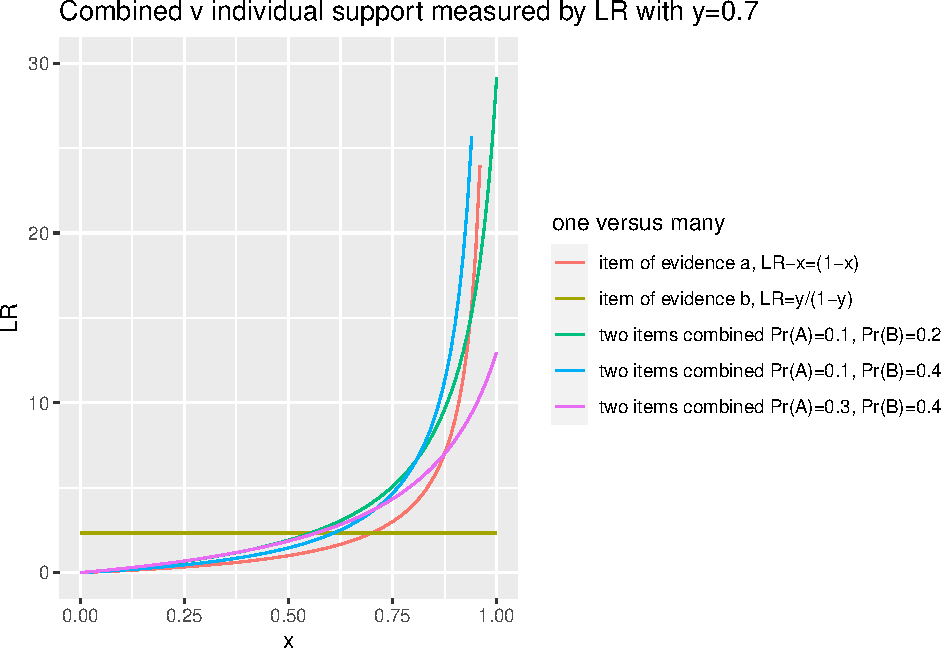
\includegraphics{BNfiles/unnamed-chunk-2-1} \end{center}
%
The \emph{ancestors} of a node \(X\) are all those nodes from
which we can reach \(X\) by following the arrows going forwards. The
\textit{parents} of a node \(X\) are those for which we can do this in one step.
The \textit{descendants} of \(X\) are all which can be reached from \(X\) by
following the arrows going forward. The \textit{children} are those for
which we can do this in one step. In the example,
$H$ is the parent (and ancestor) of both $ W$ and $BT$, which are its children (and descendants). There are no non-parent ancestors or non-children
descendants. %For more non-trivial examples, read on.

The variables, which are represented by nodes and are connected by arrows, stand in relation of probabilistic dependence. To describe these relations, 
the graphical model is accompanied by conditional probability tables. %(CPTs). 
For parentless nodes such as $H$, the tables specify 
the prior probabilities of all their possible states. Assuming $H$ stands for a binary random variable, with two possible states, 
the prior probabilities 
could be:
%
\begin{table}[H]
\centering
\begin{tabular}{lr}
\toprule
  & Prior\\
\midrule
H=murder & .01\\
H=no.murder & .99\\
\bottomrule
\end{tabular}
\end{table}
% 
\noindent
The .01 figure for H=murder rests on the assumption that, absent any incriminating evidence, the defendant is unlikely to be guilty. For children nodes, the tables specify their conditional probability given combinations of their parents' states.  If the variables are  binary, an assignment of values for them could be:
%
\begin{table}[H]
\centering
\begin{tabular}{lrr}
\toprule
  & H=murder & H=no.murder\\
\midrule
W=seen & .7 & .4\\
W=not.seen & .3 & .6\\
\bottomrule
\end{tabular}
\end{table}

\begin{table}[H]
\centering
\begin{tabular}{lrr}
\toprule
  & H=murder & H=no.murder\\
\midrule
BT=match & 1 & .063\\
BT=no.match & 0 & .937\\
\bottomrule
\end{tabular}
\end{table}
%
\noindent
%These numerical assignments are natural. 
According to the tables above, even if the defendant is not the culprit, the eyewitness testimony would still incriminate him with  probability of .4, while the blood evidence with  probability equal to only .063. The blood type frequency estimate is realistic \citep[141]{lucy2013introduction}, and so are the conditional probabilities for the eyewitness identification. 
As expected, eyewitness testimony is assumed to be less trustworthy than blood match evidence  \citep[but for complications about assessing eyewitness testimony, see][]{wixted2017RelationshipEyewitnessConfidence, Urbaniak2020Decision}.

The three probability tables above are all that is needed to define the probability distribution. The tables do not specify probabilistic dependencies between nodes that are not in a relation of child/parent, such as $BT$ and $W$. Since there is no arrow between them, nodes $BT$ and $W$ are assumed to be independent conditional on $H$, that is, $\pr(W \vert H)=\pr(W \vert H \wedge BT)$. This fact represents, as part of the structure of the network, the independence between eyewitness testimony and  blood evidence. A generalization of this fact
is the so-called Markov condition (see the textbook by \cite{neapolitan2004learning} and the supplement on Bayesian networks of the entry on Artificial Intelligence.\footnote{Available at \url{https://plato.stanford.edu/entries/artificial-intelligence/bayesian-nets.html})})

While the Bayesian network above---comprising a directed acyclic graph along with probability tables---is simple, a correct intuitive assessment of
the probability of the hypothesis given the
evidence is already challenging. Try to guess the probability that the defendant committed the murder (H=murder) given 
the following states of the
evidence:

\begin{itemize} 
\item The suspect's blood type matches the crime stain but  information about the witness is unavailable.
%\item The witness says they saw the suspect near the crime scene but information about the suspect's blood type is unavailable.
\item The suspect's blood type matches the crime stain but the witness says they did not see the suspect near the crime scene.
\item The suspect's blood type matches the crime stain and the witness says they saw the suspect near the crime scene.
%\item The witness says they saw the suspect near the crime scene but the suspect's blood types does not match the crime stain. 
\end{itemize}

%\todo{Slightly reformulated these points to emphasize it's testimonial evidence.}

\noindent Already at this level of complexity, calculations by hand become cumbersome. In contrast,  software for Bayesian networks \citep[see, for example, the $\textbf{\textsf{R}}$
package  $\textbf{\textsf{bnlearn}}$ developed by Marco Scutari and described in][]{Scutari2015Bayesian-Networ}
will easily give the following results: 
%
% (rows correspond to varioussettings of evidence, the right-most column contains the posterior
%
\begin{table}[H]
\centering
\begin{tabular}{lr}
\toprule
  & H=murder\\
\midrule
BT=match,W=? & .138\\
%BT=?, W=seen & 0.017\\
BT=match,W=not.seen & .074\\
BT=match, W=seen & .219\\
%BT=no.match, W=seen & 0.000\\
\bottomrule
\end{tabular}
\end{table}
%
\noindent
Perhaps surprisingly the posterior probability of $H$ is about .22 even when both pieces of evidence are incriminating (BT=match, W=seen).
%
\todo{Reminder: Upload the R files  with the calculations to a github folder if the entry gets published.}
%\todo{Sure I can set up a git hub project later if the entry gets accepted, please remind me about this.} 
%
%Humans are decent at identifying features
%of reality that are important for a given problem, but terrible at
%aggregating the information they have. This is where
%Bayesian networks can be of service. Humans will construct an acyclic graph according to their domain knowledge and specify conditional probabilities about parent and children nodes. Automated calculations will do the rest. 

%Besides the possibility of relying on software to do the calculations, Bayesian networks
% significantly reduce the amount of information to be stored,   since they satisfy the so-called \emph{Markov condition}. This condition means that any random variable in the network, conditional on its parents, is independent of all other variables except possibly its descendants.
%If a probability measure \(\pr{}\) and directed acyclic graph DAG \(\mathsf{G}\) satisfy this condition, we say that \(\pr{}\) is compatible with \(\mathsf{G}\) (or that the tuple \((\pr{},\mathsf{G})\) satisfies the . If \(\pr\) is compatible with
%\(\mathsf{G}\), %we do not have to represent it directly by listing joint probabilities for all the \(2^n-1\) combinations of the values of the random variables involved.  Instead, 
%If the Markov condition holds, the joint probability distribution of the variables in the Bayesian network, 
%\(\pr(X_1\dots,X_n)\), can be expressed in a more succinct way taking advantage of the independence between variables.  
%Specifically:  order all the random variables in the Bayesian network ancestrally (that is, pick an ordering in which if $Z$ is a descendant of $X$, then $Z$ comes after $X$ in the ordering), so that you obtain an ordered  sequence $X_1, \dots, X_n$. Take any selection of values of the random variables in a network, denoted by lower case $x_1, \dots, x_n$. Let $\mathsf{pa_i}$ be the set containing all the values of the parents of $X_i$ that belong to this sequence. Since this is an ancestral ordering, the parents have to occur before $X_i$. Then, it turns out that the joint probability of this selection of values can be calculated by conditionalizing on parents only:
%\begin{align*}\pr(x_n, x_{n-1}, \dots, x_1) = \pr(x_n\vert \mathsf{pa_n})\pr(x_{n-1}\vert \mathsf{pa_{n-1}})\cdots \pr(x_1)\label{eq:markoproof1}\end{align*}
%\noindent For this reason,  if the $n$ random variables are binary and each node has at most \(k\) parents, at most \(2^kn\) values are needed to specify the joint distribution. For an  introduction to Bayesian networks and further details, see the textbook by \cite{neapolitan2004learning} and the supplement on Bayesian networks of the entry on Artificial Intelligence.\footnote{Available at \url{https://plato.stanford.edu/entries/artificial-intelligence/bayesian-nets.html}).} %For an introduction to Bayesian networks using the programming language \textbf{\textsf{R}}, see .} 


\subsection{Idioms} 

Simple graphical patterns (called \emph{idioms}) often recur while modeling the relationships between evidence and hypotheses. Complex graphical models can be created by combining these basic patters 
in a modular way. Discussion of general methods for Bayesian network constructions can be found in \citep{neil2000BuildingLargescaleBayesian},
\citep{hepler2007ObjectorientedGraphicalRepresentations} and general idioms are discussed in \citep{fenton2013GeneralStructureLegal}. A few of the basic idioms
%---such as evidence, evidence accuracy, opportunity and motive, alibi and evidence dependence---
are illustrated below.

The \emph{evidence idiom} is the most basic graphical representation of the relation between a hypothesis and a piece of evidence:

\begin{center}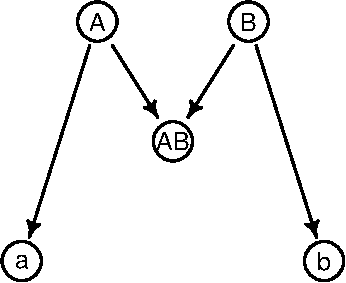
\includegraphics{BNfiles/unnamed-chunk-6-1} \end{center}

\noindent 
This directed graph suggests that the direction of influence---which could, but need not, be interpreted as causal influence---goes from hypothesis to evidence (though the probabilistic dependence goes both ways). 
The hypothesis node and the evidence node can be binary variables, such as
`The defendant was the
source of the crime scene traces' (hypothesis) and `The defendant genetically matches the crime traces' (evidence). But the variables need not be binary. The hypothesis node might take values from the range of \(1-40\), say the distance in meters from which the gun was shot, and the evidence node might be a continuous variable representing the density of gun shot residues  %See %sections 7.4.4.2 and 7.4.4.3 of
\citep{taroni2006bayesian}.


%Other idioms handle evidence accuracy, the role of opportunity,
%dependency between items of evidence, or alibi. We'll go over them
%briefly, and then we'll turn to the use of BNs in modelling fairly
%comwplete cases. Finally, we'll briefly discuss the use of BNs in DNA
%evidence evaluation.

A more complex idiom, called the \emph{evidence accuracy
idiom}, consists of two arrows going into the evidence node \citep{bovens2004bayesian, friedman1974}. One incoming arrow comes from the hypothesis node and the other from the accuracy node. This idiom can be used to model, say, 
an alcohol test:
%
\begin{center}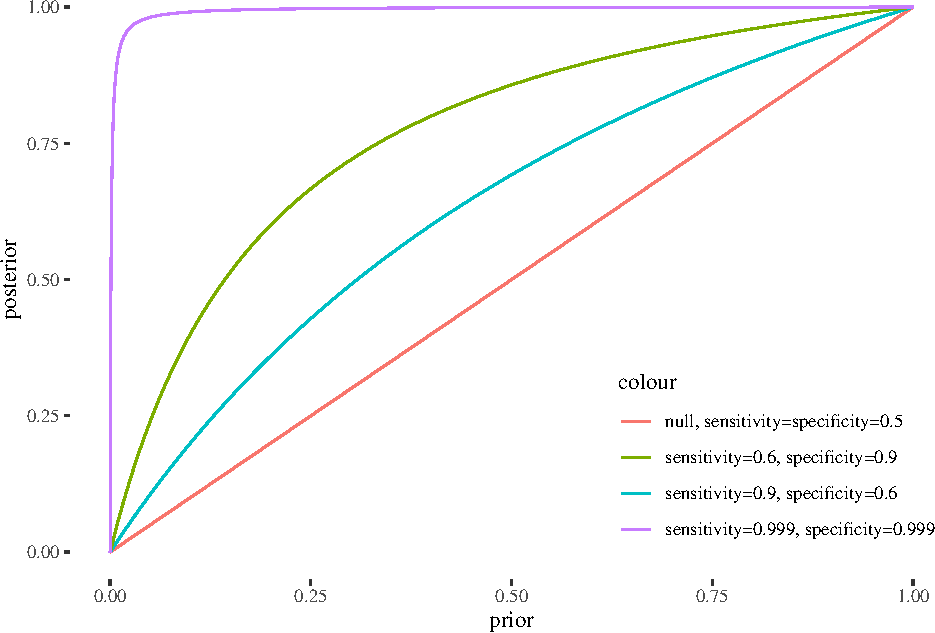
\includegraphics{BNfiles/unnamed-chunk-7-1} \end{center}
%
\noindent The directions of the arrows indicate that the accuracy of the evidence (accuracy node) and the alcohol level (hypothesis node) influence the outcome of the test (evidence node). The graphical model represents different sources of uncertainty. The uncertainty associated with the sensitivity and specificity of the test---that is, the probability that the tests reports excessive alcohol level when the level is excessive (sensitivity) and the probability that the test reports normal alcohol level when the level is normal (specificity)---is captured by the arrow  going from the hypothesis node (\textsf{Excess alcohol level}) to the evidence node (\textsf{Evidence for excess}). Other sources of uncertainty comprise the possibility that the police officer lied about the test report or
%wat's the probability that she lied if the subject was a random driver? What's 
%the probability that the driver had alcohol in his mouth which he didn't swallow? What's 
the possibility that the driver took medications which then affected the alcohol level. These possibilities can be taken into consideration by adding an accuracy node (or multiple accuracy nodes, if each factor is kept separate from the other).

%The relevant conditional probabilities pertaining to these different sources of uncertainty---such as sensitivity, specificity, lying, misinterpretation---are stored in the conditional probability tables that go with the graphical network.


%Another idiom concerns  \textit{opportunity} and \textit{motive}. Establishing someone's opportunity to commit the crime, say proximity to the victim at some point, is a necessary requirement for establishing guilt. Similar considerations apply to the notion of motive. Since both opportunity and motive are precursors to the crime, they can be modeled as parent nodes to the node representing the main hypothesis.
% Below is an example in which the opportunity idiom is combined with  two instances of the evidence accuracy idiom seen previously:


%\begin{center}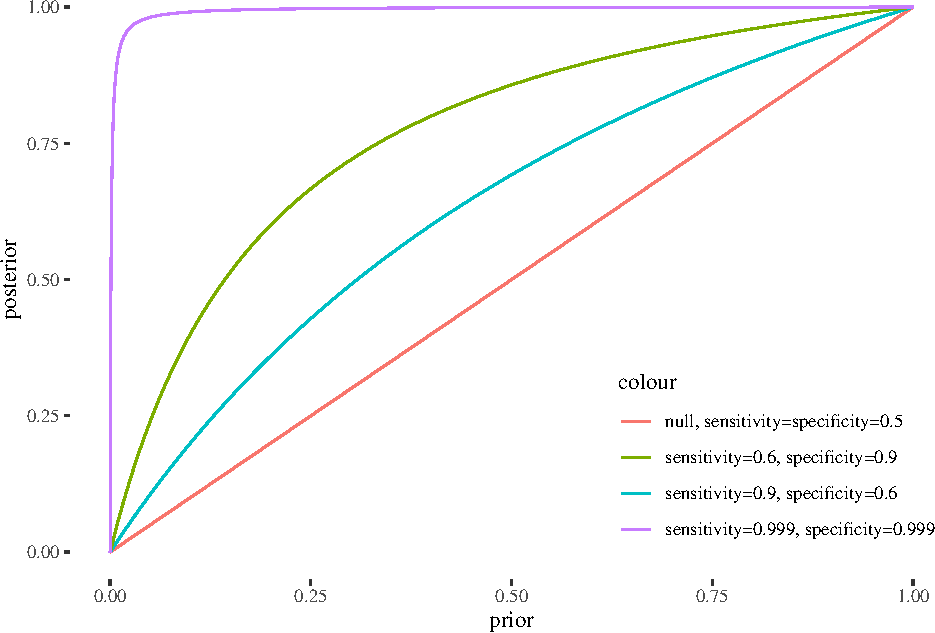
\includegraphics{BNfiles/unnamed-chunk-8-1} \end{center}

%\begin{center}
%\begin{tabular}{@{}ll@{}}
%\toprule
%Node &  Proposition\\
%\midrule
% H1 &  Defendant present at the scene \\
% H2 &  Defendant's guilt \\
% A1 & Accuracy of eyewitness evidence\\
% A2 & Accuracy of security camera evidence \\
% E1 & Eyewitness testimony \\
% E2 & Evidence from security camera\\
%\bottomrule
%\end{tabular}
%\end{center}

%\noindent
%The opportunity node (H1) is the parent of the node representing the main hypothesis (H2). 


When multiple items of evidence depend on one another---as may happen in many legal cases---this situation is modelled by the \textit{evidence dependency idiom}. Following an example by \cite{Fenton2018Risk}, if one of two security cameras directed at the same location captured an image of someone who looks like the defendant but isn't him, it is likely that the same person walked by the second camera, which also captured the same image. In such cases, presenting the second recording as independent from the first would lead to overestimating the strength of the evidence.   %\citep[421]{Fenton2018Risk}. 

\begin{center}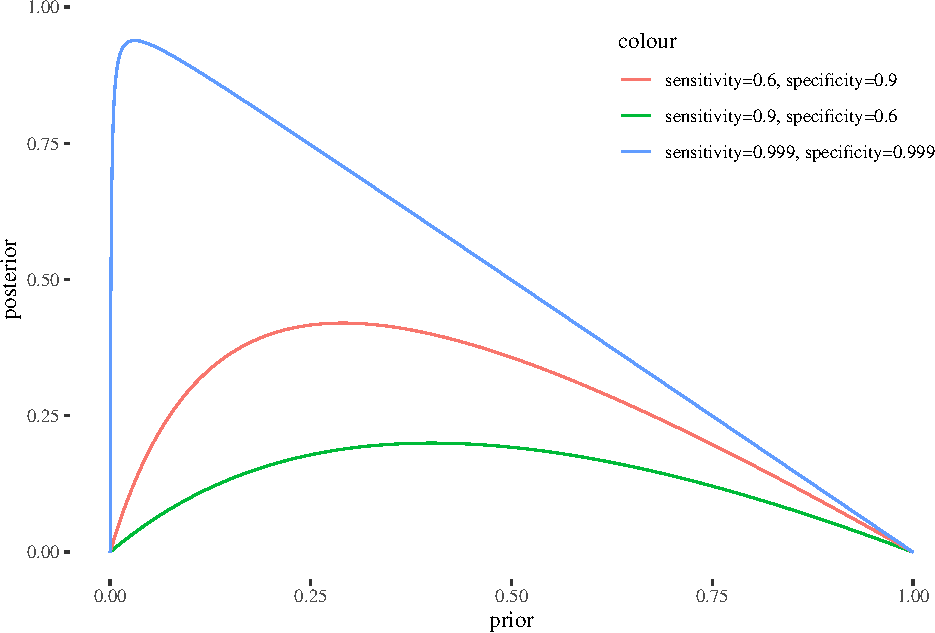
\includegraphics{BNfiles/unnamed-chunk-9-1} \end{center}

\begin{center}
\begin{tabular}{@{}lp{7.5cm}@{}}
\toprule
Node &  Proposition\\
\midrule
H &  Defendant present at the scene \\
C1 & Camera 1 captures image of a matching person \\
C2 & Camera 2 captures image of a matching person\\
D &  What cameras capture is dependent \\
\bottomrule
\end{tabular}
\end{center}


\noindent The network structure is quite natural. The truth of the hypothesis, say, the defendant was present at the crime scene, influences whether the cameras capture an image of someone who looks like the defendant. However, if the two camera recordings are dependent on one another (for instance, they are directed at the same spot with a similar angle), the fact that the second camera captured the same image as the first does not make the hypothesis more likely once the first camera recording is known.

%Another common pattern is the \emph{alibi idiom}. An alibi testimony serves to argue that the defendant was not at the  scene when the crime occurred. %One slightly tricky issue is that 
%An alibi testimony, if truthful, would contradict the prosecutor's hypothesis. Conversely, the prosecutor's hypothesis, if correct, would undermine the veracity of the alibi testimony.
%itself may have impact on the accuracy of the evidence (for instance if the eyewitness is a friend of the defendant). The question is, 
%The challenge is to model this interplay between alibi testimony and prosecutor's hypothesis without using a cyclic graph. Here is a proposal by \cite{lagnado2013legal}: 

%\begin{center}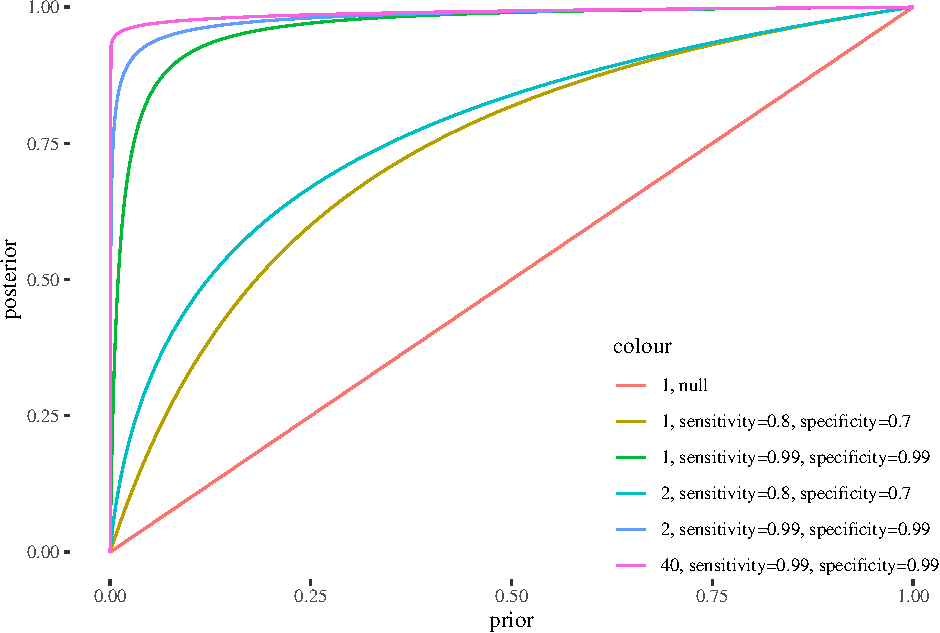
\includegraphics{BNfiles/unnamed-chunk-10-1} \end{center}

%\noindent
%The arrow goes from \textsf{S present} to \textsf{Alibi} because whether or not the suspect was present at the scene affects the veracity of the alibi testimony. Further, an arrow goes from \textsf{S present} to \textsf{S guilty} because whether or not the suspect was present at the scene influences whether or not he is guilty. Another arrow goes from \textsf{S guilty} to \textsf{Alibi accuracy} because whether or not the suspect is guilty influences the accuracy of the alibi testimony, which in turn, affects the alibi testimony. As desired, this graphical model captures  the interplay between alibi testimony and prosecutor's hypothesis without using a cyclic graph.

%\subsection{Scenarios}

% \todo{M: Shortened this bit, removed alibi idiom and motive idiom, and moved the scenario idioms up before Sally Clark. Also, removed the more complicated bit about merging scenarios and constraints}

%As we discuss elsewhere in this entry, somecritics of legal probabilism insist that the key notion used in thinking
%about legal evidence evaluation is that of a narration, and that it is a
%flaw of the probabilist toolkit that it can't capture it. To counter
%this pressure, and to apply BNs to the assessment of whole cases, it is
%worthwhile to see that the Bayesian toolkit does have the potential to
%capture narration-related notions. Or at least the proponents the
%methodology think so (see the discussion of literature included in this
%section). Let us take a brief look.


%In complex criminal cases, prosecution and defense make their case by advancing a coherent presentation of a sequence of events (called a \emph{scenario}). For example, the prosecutor may put forward the following sequence of events: the defendant had a fight with the victim; a knife was lying on the kitchen counter; the victim said something insulting, so the defendant took the knife and stabbed the victim. 
%The defense may instead advance a different version of what happened: 
%the defendant had a fight with the victim; a knife was lying on the kitchen counter; the victim became aggressive and was about to stab the defendant to death who had no other choice than to stab the victim in self-defense. 



Finally, the \textit{scenario idiom} can model  complex hypotheses, consisting of a sequence of events organized in space and time (a scenario). A graphical model that uses the scenario idiom would consist of the following components: first, nodes for the states and events in the scenario, with each node linked to the supporting evidence; second, a separate scenario node that has states and events as its children; finally, a node corresponding to the ultimate hypothesis as a child of the scenario node. The graphical 
model would look like this %A discussion of representing  scenarios by means of Bayesian networks can be found in 
\citep{vlek2014building}:
%and \citep{vlek2016stories}.:

%
\begin{center}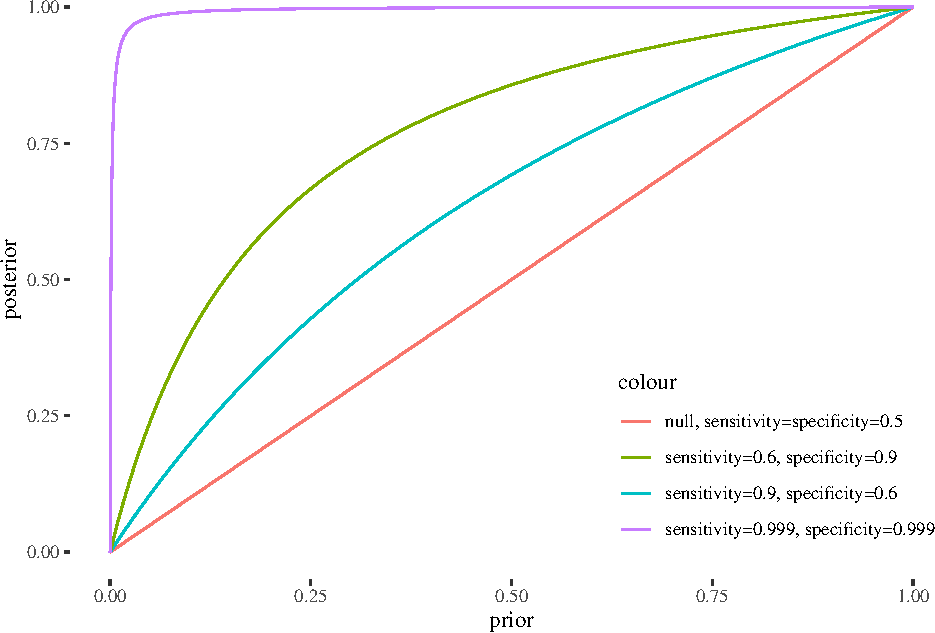
\includegraphics{BNfiles/unnamed-chunk-13-1} \end{center}


%Following some guidelines,  model such the consideration of the interplay of such scenarios given the available evidence. The basic guidelines are as follows:

%\begin{itemize}
%\item 
%\item For each state and event mentioned in a scenario, and for each piece of evidence, include a binary node in the Bayesian network and connect them as appropriate. 
%\item Add a binary scenario node as a parent of all the elements of the scenario, and a guilt hypothesis node as its child.  
%\end{itemize}


\noindent
 The scenario node unifies the different events and states.  
 %\todo{Are you sure each child takes values one if the scenario node has value one? Or is this limited to each child that is a state/event node?}
 %Each child of the scenario node should take value \textsf{true} if the scenario node takes value \textsf{true}, and the conditional probability of the node, \todo{What does it mean "probability of the node"? Isn't the probability about the node/variable taking a certain value?}given that the scenario node takes value \textsf{false}, should equal its prior probability in the network before the scenario idiom was added. 
 Because of this unifying role, increasing the probability of one part of the scenario (say \textsf{State/event 2}) will also increase the probability of the other parts (\textsf{State/event 1} and  \textsf{State/event 3}). This captures the fact that  the different components 
 of a scenario form an interconnected sequence of events. 
 

%
%Now, once multiple scenarios have been proposed, at least in some cases,they can be merged to construct a larger BN in which each of the scenarios can be evaluated.
%
%Each scenario node can also be merged with other scenario nodes to form a larger Bayesian network.  To merge two scenarios, put their
%corresponding Bayesian network together and if some nodes in the scenarios are identical (including the guilt nodes), replace them with a single node.
%
%\begin{center}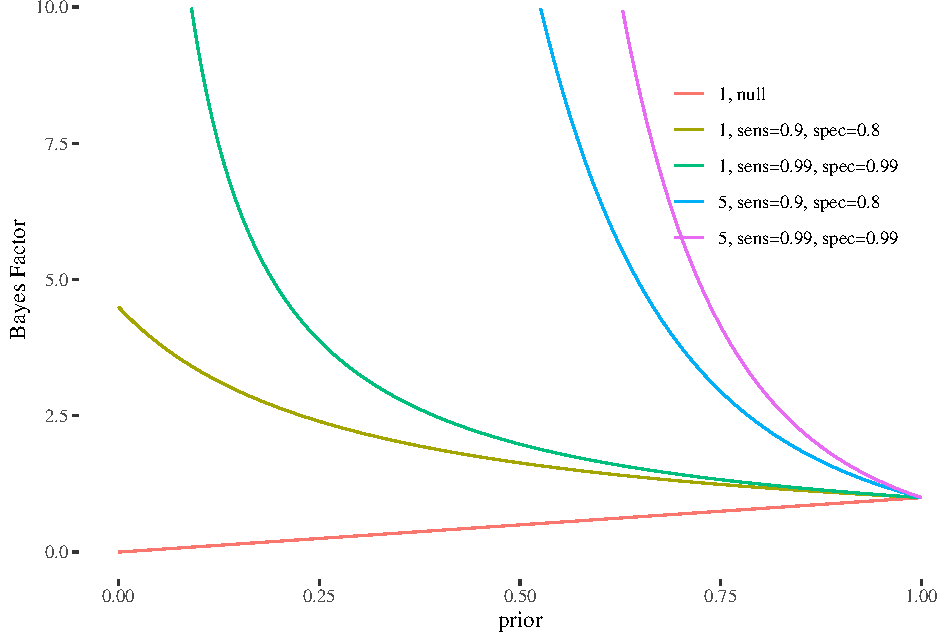
\includegraphics{BNfiles/unnamed-chunk-15-1} \end{center}
%
%The guilt node will have arrows going in from different  scenario nodes. The probability of the guilt node taking value \textsf{true} will depend on the values assigned to the scenario nodes. 
%Some scenarios nodes will have to take value  \textsf{true} and others value \textsf{false} in order for the guilt node to take value \textsf{true}.
%This will depend on the specifics of each case and the relationship between scenarios and ultimate hypothesis. 
%Different scenarios  will support different values of the ultimate hypothesis, for example, 
%Some scenario (if true) will make the defendant's guilt more probable and other scenarios (if true) will make it less probable. 
%It may be that a scenario node excludes another, say, one scenario asserts that the defendant was at home while the crime occurred and another asserts the defendant participated in the crime. For any two scenario nodes that exclude one another, a constraint node can be added with values \textsf{allowed} and \textsf{not allowed}. 
%
%\begin{center}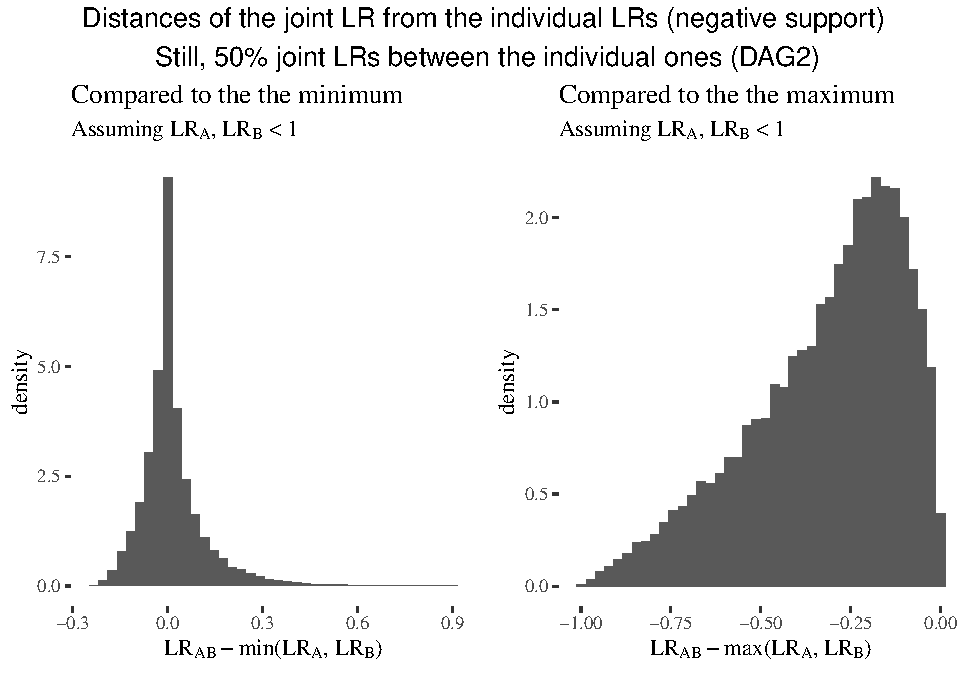
\includegraphics{BNfiles/unnamed-chunk-14-1} \end{center}
%
%\noindent
%The constraint node takes values 
%\textsf{allowed} just in case exactly one of the scenario nodes takes value 
%\textrm{true}, and \textsf{not allowed} otherwise.
%The idea is that we make sure the scenarios exclude each other.
%

%When the different scenarios are combined along with the appropriate constraint nodes, the relations of dependency between the  scenarios can be studied. This feature, however, might be undesirable if one does not 
%want other elements of the scenario to become more probable simply because  one element of the scenario is supported by the evidence.
%

A discussion
of modelling crime scenarios by means of other graphical devices (called structural scenario spaces) mixed with probabilities can be found in the work of 
\cite{shen2007ScenariodrivenDecisionSupporta}, \cite{bex2011ArgumentsStoriesCriminal, bex2015IntegratedTheoryCausal} and
\cite{verheijproof2017}.
See also the survey by \citet{di2018evidential}.
\cite{dawid2018graphical} 
give a treatment of scenarios in terms of  Bayesian networks. \cite{lacave2002ReviewExplanationMethodsa} show how Bayesian Network can be used to construct explanations.

%\citep[see also][for such issues]{vlek2016method}. 













%\subsection{BNs for DNA evidence evaluation} \label{subsec:BNSforDNA}

%Bayesian networks can be used 
%for assessing DNA evidence in  complex cases. 
%While it does not really involve idioms and is not a modelof the whole case, it nicely illustrates the utility of BNs in legalevidence evaluation. 
%DNA profiling relies on genetic differences between individuals 
%in small regions (loci) of the human genome. At select loci, called Short Tandem Repeat (STR) loci, sequences of base pairs are repeated multiple times. Each STR locus is associated with a few possible mutations (alleles) differentiated by the number of base pair repeats at that locus.   
%The length of a repeated sequences expressed as thenumber of repeats in the sequence i
%s called an allele. 
%For any individual, the two 
%alleles at a given STR locus are 
%inherited from one's parents and constitute the genotype at that locus, which can be described by a pair of two numbers, say (8, 7). 
%A specific genotype at a locus is 
%normally shared by 5-15\% of the population. 
%At each locus
%there are two alleles, inherited from the parents. 
%So a particular locus
%can be described in terms of two numbers, the The genotype of that locus.
%The two alleles can be the same (the person is then homozygous at that locus)
%or different (the person is then heterozygous). 
%Normally, a genotype at
%a given locus is shared by 5-15\% of the population. 
%
%DNA profiling relies on 
%a selection of STR loci (often 17 or 20). The estimated frequency of a DNA profile is obtained 
%by multiplying the frequencies of the genotypes at the select loci. The multiplication rests on the assumption of the independence of the STR loci \citep{Kaye2010The-Double-Heli}.

%In standard DNA evidence cases, the crime scene sample matches with the defendant at all the available loci. % What happens in many cases, however, is more complicated. %If people are related,
%they are more likely to share genotypes.
%But sometimes the sample
%from the crime scene is of low quality and only a subset of the usual
%loci can be used. Or a profile can be mixed and comprise genetic material from more than one individual. For instance, suppose that after analyzing the crime traces three different alleles are found at locus TH01 (say, alleles 7,8 and 9). If the defendant has genotype (7,7), could the defendant be the source?
%Different combinations are possible (and only one of them does not exclude the suspect as a source):

%
%\begin{center}
%\begin{tabular}{@{}ll@{}}
%\toprule
%Contributor 1 (C1) & Contributor 2  (C2)
%\\ \midrule (7,7) & (8,9)\\
%(7,8) & (8,9)\\
%(7,8) & (9,9)\\
%(7,8) & (9,9)\\
%(8,8) & (7,9)\\ \bottomrule
%\end{tabular}
%\end{center}
%
%The following Bayesian network can be
%used to properly evaluate this piece of evidence \citep{weir1997interpreting, cowell2011ProbabilisticExpertSystems}:
%
%\begin{center}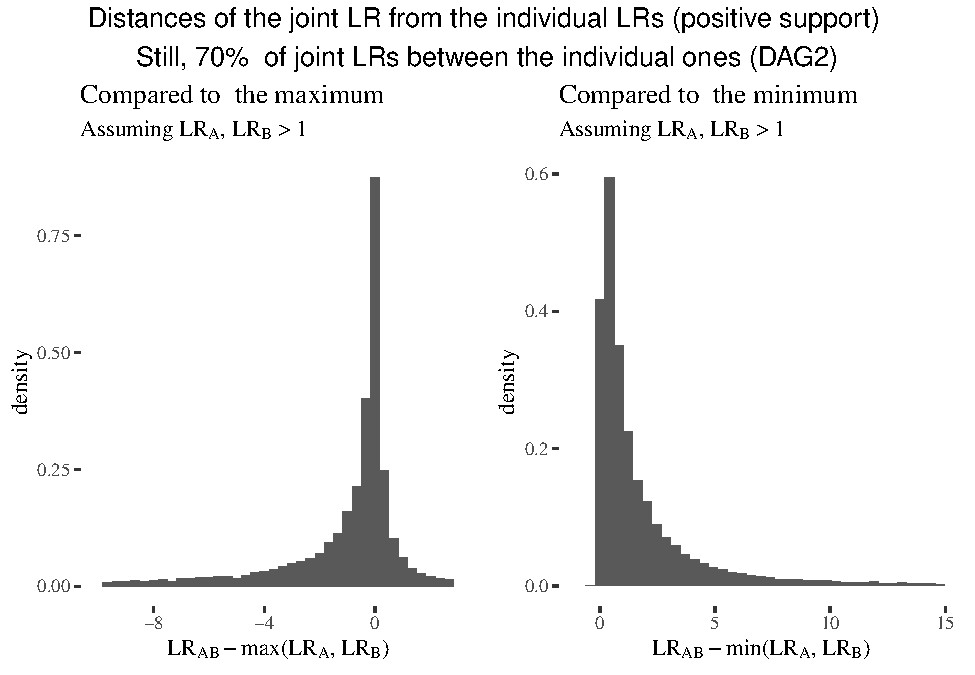
\includegraphics{BNfiles/unnamed-chunk-16-1} \end{center}

%\noindent
%Calculations show that the evidence causes only a small increase in the probability of the hypothesis that the suspect is the source of the genetic material, from 50\% to 62.5\%.
%
%An application of Bayesian networks to the evaluation of scientific evidence (fibre
%and blood evidence) and disputed paternity cases is discussed in 
%\citep{dawid1997using} and \citep{dawid1999inference}. 
%The BN handling of the complexity involved
%in mixed DNA evidence evaluation is discussed in
%\citep{weir1997interpreting}, and later on in
%\citep{cowell2011ProbabilisticExpertSystems}. 
%Bayesian networks are also used to analyze 
% transfer probabilites  \citep{garbolino2002evaluation}  
%and cross-transfer evidence 
%\citep{aitken2003GraphicalModelEvaluation}.

%(transfer probabilities are  probabilities that a subject's genetic material gets transferred to the sample given various scenarios of what happened).


%\subsection{Historical remarks and literature on BNs for legal applications}

%\todo{Marcello: Can't we sprinkle these references here and there earlier? Having all of them concentrated here seems abut too much.}

%\todo{I prefer not to; 1) The presentation of BNs is a bit jittery as it is, interrupting it with references would disrupt the flow even more. 2) some of the things I mention played important part in the developments but I don't talk about their results directly so there is no natural point to mention them. 3) I don't think there's anything wrong with a literature survey section. I propose a change in the section title, think if it helps.}


%The idea that BNs can be used forprobabilistic reasoning in legal fact-finding started gaining tractionin late eighties \citep{Friedman1986A-diagrammatic-} and early nineties
%More advanced steps in thisdirection soon followed. An application of BNs to the evaluation ofscientific evidence is discussed by \citet{dawid1997using} use BNs to model examples of the evaluation of particular items of evidence (fibre and blood evidence), and extend this work to disputed paternity cases
%\citep{dawid1999inference}. The BN handling of the complexity involved
%in mixed DNA evidence evaluation is discussed in
%\citep{weir1997interpreting}, and later on in
%\citep{cowell2011ProbabilisticExpertSystems}. BNs are used to discuss
%the role of transfer probabilites in \citep{garbolino2002evaluation},
%and cross-transfer evidence is discussed in terms of BNs in
%\citep{aitken2003GraphicalModelEvaluation}. Discussion of general
%methods for BNs constructions can be found in
%\citep{neil2000BuildingLargescaleBayesian},
%\citep{hepler2007ObjectorientedGraphicalRepresentations} and general
%idioms are discussed in \citep{fenton2013GeneralStructureLegal}.
%\citep{lacave2002ReviewExplanationMethodsa} contains a discussion of how
%BNs can be used to construct explanation
%\citep[see also][for such issues]{vlek2016method}. A nice survey of
%these issues is a chapter of \citep{Fenton2018Risk}. A comperehnsive
%book on the topic is \citep{taroni2006bayesian}. One issue that arises
%is how to elicit quite a few probabilities: these issues are discussed
%in \citep{renooij2001ProbabilityElicitationBeliefa} and
%\citep{gaag2013elicit}.

%Using BNs to evaluate pieces of evidence is one thing, using them to
%capture whole crime scenarios is another. One such study of a particular
%famous case is \citep{kadane2011probabilistic}. A more general treatment
%of modelling crime scenarios in terms of graphical devices (so called
%structural scenario spaces) mixed with probabilities can be found in
%\citep{shen2007ScenariodrivenDecisionSupporta},
%\citep{bex2011ArgumentsStoriesCriminal},
%\citep{bex2015IntegratedTheoryCausal}, and in the works of Verheij
%\citep{verheij2007argumentation,verheij2014catch,verheij2015arguments,verheijproof2017}.
%See also the survey by %\citet{di2018evidential}.
%\citep{dawid2018graphical} contains a treamtent of scenarios more
%focused on BNs, and extensive discussion of representing crime scenarios
%by means of BNs can be found in the works of Vlek
%\citep{vlek2013modeling,vlek2014building,vlek2016stories}.




 




 
 







\subsection{Modeling an entire case}\label{subsec:completeBN}

%Using Bayesian networks to evaluate pieces of evidence is one thing, using them to
%model entire legal cases is quite another. 
\cite{kadane2011probabilistic}
made one the first attempts to model an entire criminal case, Sacco \& Vanzetti from 1920, using probabilistic graphs. More recently, \cite{Fenton2018Risk} constructed a Bayesian network for the Sally Clark case (discussed earlier in~\ref{sec:odd-bayes}), reproduced below:

%For the details of the construction, see  \citep{Fenton2018Risk}, here we will simply present the result of the analysis. 

%
\begin{center}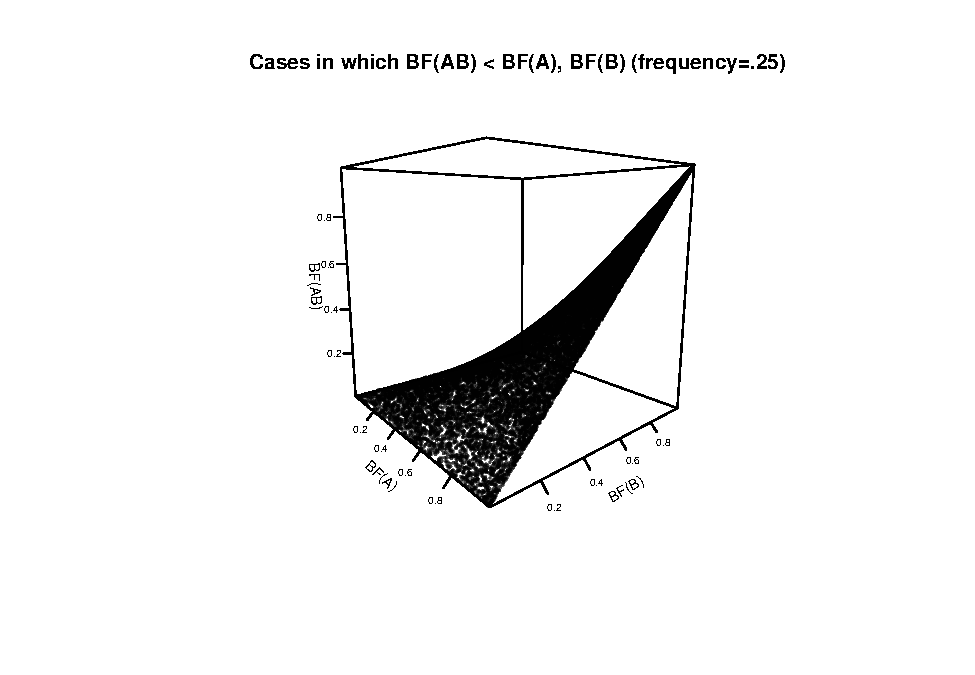
\includegraphics{BNfiles/unnamed-chunk-11-1} \end{center}

\noindent
%Most nodes in the diagram correspond to binary 
%variables: the cause of death is either Sudden Infant Death Syndrome (SIDS)
%or murder; bruising on Sally Clark's sons is either present or not; signs of a disease affecting the two sons are either present or not; 
%Sally Clark is either guilty or not. 
%For Sally Clark's two sons, call them \(A\) and \(B\), etc. %. 
%The exception 
%is the node \textsf{No.murdered} that represents how many of Clark's sons were murdered. This node takes one of three values: \(0, 1, 2\).
%
The arrows depict relationships of influence between variables. Whether Sally Clark's sons, call them \(A\) and \(B\), died by SIDS or murder (\textsf{A.cause} and \textsf{B.cause}) influences whether signs of disease (\textsf{A.disease} and \textsf{B.disease}) and bruising (\textsf{A.bruising} and \textsf{B.bruising})  were present. % Clark's sons, A and B. 
%The arrows goes from the node \textsf{A.cause} to the nodes
%\textsf{A.bruising} and \textsf{A.disease}. Similarly, the arrows goes from the node \textsf{B.cause} to the nodes
%\textsf{B.bruising} and (\textsf{B.disease}
Since son A died first, whether A was murdered or died by SIDS (\textsf{A.cause}) influences how son B died (\textsf{B.cause}). 
%Accordingly, the arrows goes from the node \textsf{A.cause} to the node \textsf{B.cause}. 
How the sons died %(by SIDS or murder) 
determines how many sons were murdered (\textsf{No.murdered}), and how many sons were murdered decides whether Sally Clark is guilty (\textsf{guilty}). 


According to the calculation by \cite{Fenton2018Risk} (see their paper for details), the prior probability of \textrm{Guilty = Yes} should be .0789. After taking into account the incriminating evidence presented at trial, such as that there were signs of bruising but no signs of a preexisting disease affecting the children, the posterior probabilities are as follows:

\begin{center}
\begin{tabular}{@{}ll@{}}
\toprule
Evidence (cumulative) & $\pr(\textrm{Clark guilty})$ 
\\ \midrule 
A bruising& .2887\\
A no signs of disease & .3093\\
B bruising & .6913\\
B no signs of disease  & .7019\\
 \bottomrule
\end{tabular}
\end{center}

\noindent 
The incriminating evidence, combined, brings the probability of guilt from .0789 to .7019. This is a significant increase, but not quite enough for a conviction. If one wishes to perform sensitivity analysis---see earlier discussion in \ref{subsec:sensi-ana}---by modifying some of the probabilities, this can be easily done.
%
During the appeal trial, new evidence was discovered, in particular, evidence that son A was affected by a disease. 
Once this evidence is taken into account, the probability of guilt drops to .00459  (and if signs of disease were also present on B, the guilt probability would drop even further to .0009). For a general discussion on how to elicit probabilities, see \citep{renooij2001ProbabilityElicitationBeliefa} and
\citep{gaag2013elicit}.





%propose the following conditional probability tables:

%\begin{table}[H]
%\centering
%\begin{tabular}{lr}
%\toprule
%  & Cause of death of child A\\
%\midrule
%A.cause=SIDS & 0.921659\\
%A.cause = Murder & 0.078341\\
%\bottomrule
%\end{tabular}
%\end{table}

%\begin{table}[H]
%\centering
%\begin{tabular}{lrr}
%\toprule
%  & A.cause = SIDS & A.cause = Murder\\
%\midrule
%A.bruising = Yes & 0.01 & 0.05\\
%A.bruising = No & 0.99 & 0.95\\
%\bottomrule
%\end{tabular}
%\end{table}

%\begin{table}[H]
%\centering
%\begin{tabular}{lrr}
%\toprule
%  & A.cause = SIDS & A.cause = Murder\\
%\midrule
%A.disease = Yes & 0.05 & 0.001\\
%A.disease = No & 0.95 & 0.999\\
%\bottomrule
%\end{tabular}
%\end{table}

%\begin{table}[H]
%\centering
%\begin{tabular}{lrr}
%\toprule
%  & B.cause = SIDS & B.cause = Murder\\
%\midrule
%B.bruising = Yes & 0.01 & 0.05\\
%B.bruising = No & 0.99 & 0.95\\
%\bottomrule
%\end{tabular}
%\end{table}

%\begin{table}[H]
%\centering
%\begin{tabular}{lrr}
%\toprule
%  & B.cause = SIDS & B.cause = Murder\\
%\midrule
%A.disease = Yes & 0.05 & 0.001\\
%A.disease = No & 0.95 & 0.999\\
%\bottomrule
%\end{tabular}
%\end{table}

%\begin{table}[H]
%\centering
%\begin{tabular}{lrr}
%\toprule
%  & A.cause = SIDS & A.cause = Murder\\
%\midrule
%B.cause = SIDS & 0.9993604 & 0.0001462\\
%B.cause = Murder & 0.0006396 & 0.9998538\\
%\bottomrule
%\end{tabular}
%\end{table}

%\begin{table}[H]
%\centering
%\footnotesize
%\begin{tabular}{lrrrr}
%\toprule
%  &\tiny  A, B= SIDS &\tiny   A = Murder, B = % SIDS & \tiny  A = SIDS, B = Murder & \tiny  A = B % = Murder\\
% \midrule
% \tiny Number.murdered = both & 0 & 0 & 0 & 1\\
% \tiny Number.murdered = one & 0 & 1 & 1 & 0\\
% \tiny Number.murdered = none & 1 & 0 & 0 & 0\\
% \bottomrule
% \end{tabular}
% \end{table}

% \begin{table}[H]
% \centering
% \begin{tabular}{lrrr}
% \toprule
%  & both & one & none\\
% \midrule
% Guilty = Yes & 1 & 1 & 0\\
% Guilty = No & 0 & 0 & 1\\
% \bottomrule
% \end{tabular}
% \end{table}

%\noindent
%Some of these numbers were assigned based on frequencies, and to some extent on  informed but subjectiveestimation. 
%\todo{added the parenthical remark} 
%The table for the 
%parentless node \textsf{A.cause} 
%contains the prior
%probabilities for its two states (SIDS, Murder) based on the estimated frequency with which children are murdered by their mother. 
%The table for the definitional nodes \linebreak  (\textsf{No.murdered} and \textsf{guilty}) contains only 0s and 1s. The numerical values for other tables reflect informed subjective priors based on expert testimony proffered during the first trial of Sally Clark. If SIDS was the cause of death, bruising is very unlikely (probability of 0.01), but signs of diseases are slightly more likely (probability of 0.05). If, instead, the cause of death was murder, signs of disease are close to impossible (probability of 0.001), but bruising is significantly more likely (probability of 0.05). These numbers apply to both child A and child B. Finally,
%if the first SIDS death occurred, the second SIDS death is estimated to be very likely (probability of 0.9993604), and if the first child was the victim of a murder, the second being murdered is extremely likely (probability of 0.9998538).
%The probabilities of the other combinations, instead, are estimated to be low. 
%For a general discussion on how to elicit probabilities, see
%\citep{renooij2001ProbabilityElicitationBeliefa} and
%\citep{gaag2013elicit}.

























\section{Relevance}\label{sec:relevance}


%\todo{This is the only section that has no subsections, should we change this?}

The preceding sections modeled evidence assessment, using  Bayes' theorem (Section \ref{sec:toolkit}), likelihood ratios (section \ref{sec:LR}) and   Bayesian networks (Section \ref{sec:BNs}). 
%The objective was to assign a posterior probability to a hypothesis of interest---say, that the defendant is guilty---given all the evidence presented at trial. 
Evidence assessment, however, begins with a preliminary decision, the identification of relevant evidence. 
%The testimony of an eyewitness who says she was around the scene at the time of the crime should count as relevant evidence. A testimony by someone who had nothing to do with the crime should not.  
%
Once a piece of evidence is deemed relevant, the next step is to assess its strength (probative value, weight). 
This section discusses how probability theory helps to identify relevant evidence.


%\subsection{Modeling relevance: likelihood ratios and Bayesian networks}

\subsection{Likelihood ratios}

The U.S.\ Federal Rules of Evidence
define relevant evidence as evidence that has `any tendency to make the existence of any fact that is of consequence to the determination of the action more probable or less probable than it would be without the evidence' (rule 401). 
This definition is formulated in a probabilistic language.
Legal probabilists interpret it using the likelihood ratio, a standard probabilistic measure of 
evidential relevance \citep{lempert1977modeling,lyon1996relevance,aitken2004statistics, aitken2010fundamentals,sullivan2016LikelihoodStoryTheory}.
The likelihood ratio (discussed in Section \ref{sec:LR}) is the probability of observing the evidence given the prosecutor's or plaintiff's hypothesis,  divided by the probability of observing the same evidence given  the defense's hypothesis. 

Let $E$ be the evidence, $H$ the prosecutor's or plaintiff's hypothesis, and $H'$ the defense's hypothesis. The likelihood ratio 
%$LR(E, H, H')$ 
is defined as follows:
%
\begin{align*}LR(E,H,H') & = \frac{P(E\vert H)}{P(E\vert H')}\end{align*}
%
On the likelihood ratio interpretation, relevance depends on the choice of the competing hypotheses. 
%$H_p$ and $H_d$ are used as examples, but other competing hypotheses $H$ and $H'$ could also be used. %When there are no ambiguities, $LR(E, H_p, H_d)$ will be shortened into the less cumbersome $LR(E)$. 
%
A piece of evidence is relevant---in relation to a pair of hypotheses $H$ and $H'$---provided the likelihood ratio  $LR(E, H, H')$ 
is different from one and irrelevant otherwise. For example, 
the bloody knife found in the suspect's home is relevant  evidence in favor of the prosecutor's hypothesis because we think it is far more likely to find such evidence if the suspect committed the crime (prosecutor's hypothesis) than if he didn't (defense hypothesis) %\citep[7]{finkelstein2009basic}
\citep{finkelstein2009basic}. In general, 
for values greater than one, $LR(E, H, H')>1$, the evidence supports the prosecutor's or plaintiff's hypothesis $H$, and for values below one, $LR(E, H, H')<1$, the evidence supports the defense's hypothesis $H'$.
If the evidence is equally likely under either hypothesis,
$LR(E, H, H')=1$, the evidence is  irrelevant. 

\subsection{The Small Town Murder objection}

This account of relevance has been challenged by cases in which the evidence 
is intuitively relevant and yet
its likelihood ratio, arguably, equals one. Here is one problematic case:
%One such case is \emph{Small Town Murder} 
\begin{quote}
	\emph{Small Town Murder:} A person accused of murder in a small town was seen driving to the small town at a time prior to the murder. The prosecution's theory is that he was driving there to commit the murder. The defense theory is an alibi: he was driving to the town to visit his mother. The probability of this evidence if he is guilty equals that if he is innocent, and thus the likelihood ratio is 1 \dots %, and under what is suggested as the ``Bayesian'' analysis, it is therefore irrelevant. 
	Yet, every judge in every trial courtroom of the country would admit it [as relevant evidence]. %, and I think everyone on this list would say it is relevant. 
	%And so we have a puzzle.  
	\citep[The difficulty has been formulated by Ronald Allen, see the discussion in][]{park2010BayesWarsRedivivus}
	\end{quote}
\noindent 
Counterexamples of this sort abound. Suppose a prisoner and two guards had an altercation because the prisoner refused to return a food tray.  The prisoner had not received a package sent to him by his family and kept the tray in protest. According to the defense, the prisoner was attacked by the guards, but according to the prosecution, he attacked the guards. The information about the package sent to the prisoner and the withholding of the tray fails to favor either version of the facts, yet it is relevant evidence \citep{pardo2013NaturePurposeEvidence}.
%Counterexamples of this sort abound.
%\begin{itemize}
%\item In response to an eyewitness testimony the defendant claims that his identical twin is the culprit. The testimony is unable to favor any of the two options and yet is considered relevant. 
%\item  Suppose the evidence at issue is that a fight occurred and the only dispute is over who started it. 
%\item 
%Or suppose the defendant was stopped because of speeding  three minutes after an aborted bank robbery and $\nicefrac{1}{2}$ a mile away from the site. The prosecution says this is evidence of guilt: it shows the defendant was escaping. The defense responds that this is evidence of innocence: no bank robber would speed and attract attention. 
%Or, in a murder case, the defendant is the victim's son. Is that relevant to show he’s guilty? Is it relevant to show he's innocent? The answer seems to be yes, to both questions. 
%This example is due to Samuel Gross 
%and is discussed in \citep{park2010BayesWarsRedivivus}. 

%In general, there seem to be  numerous examples in which evidence is, intuitively relevant, and the evidence supports neither side's theory over the other side's theory. How is such evidence to be judged relevant  from the probabilist perspective?

%\subsection{Replies to the overlapping evidence objection}

%In response (inspired by the ideas put forward in the discussion by David Kaye, Bruce Hay and Roger Park),  note that  

It is true that if a piece of evidence $E$ fits equally well with two competing hypotheses  $H$ and $H'$,  then $P(E\vert H)=P(E\vert H')$ and thus $LR(E,H,H')$ will equal 1. But the likelihood ratio may change depending on the selection of hypotheses. Rule 401 makes clear that relevant 
evidence should have `any tendency to make the existence of \emph{any fact that is of consequence} [emphasis ours] to the determination of the action more probable or less probable.' So the range of hypotheses to compare should be broad. Just because the likelihood ratio equals one for a specific selection of $H$ and $H'$, it does not follow that it equals one for \textit{any} selection of $H$ and $H'$ which are of consequence to the determination of what happened.  In \textit{Small Town Murder}, whether the suspect was in town is of consequence for determining what happened  (if he was not in town, he could not have committed the crime). The fact that he was seen driving is helpful information for establishing whether he was in town.  

But if the range of  hypotheses $H$ and $H'$ to compare in the likelihood ratio $LR(E, H, H')$ is broad, 
this may raise another concern. The choice of hypotheses  needed to determine the relevance of an  item of evidence might depend on other items of evidence, and so it might be  difficult to determine relevance until one has heard all the evidence.  This fact --- Ronald Allen and Samuel Gross argue in \citep{park2010BayesWarsRedivivus} ---  makes the probabilistic account of relevance impractical.  In response, David Kaye points out that deciding whether a reasonable juror would find  evidence $E$  helpful requires only looking at what hypotheses or stories the juror would reasonably consider. Since the jurors will rely on several clues about which stories are reasonable, this task is computationally easier than going over all possible combinations of  hypotheses \citep{park2010BayesWarsRedivivus}. 

%\subsection{Small Town Murder and bayesian networks}\label{sec:smalltownBN}

%Legal probabilists can also offer a more principled response to \emph{Small Town Murder} and related problems based on Bayesian networks.
%rather than a reasonable choice of the competing  hypotheses. 
%The emphasis on the logical relations between the hypotheses have been used by Fenton to  address the . 
%Let $H_p$ be the prosecutor's hypothesis that the defendant committed the murder, and $H_d$ the defense's hypothesis  that the defendant was visiting his mother. Let $E$ be the fact that the defendant was seen driving to town prior to the murder. Further, suppose the prior probabilities of $H_d$ and $H_p$ are $50\%$, and the conditional probability of $E$ on each of those hypotheses is $70\%$ (nothing of what will be said depends on this particular choice of values). Crucially, while the evidence supports both hypotheses, this example is based on a pair of hypotheses that are neither mutually exclusive nor exhaustive. A Bayesian network can be used to calculate other likelihood ratios for hypotheses that are exclusive and exhaustive. 

%
%\begin{figure}[h!]
%	\begin{floatrow}
%		\ffigbox{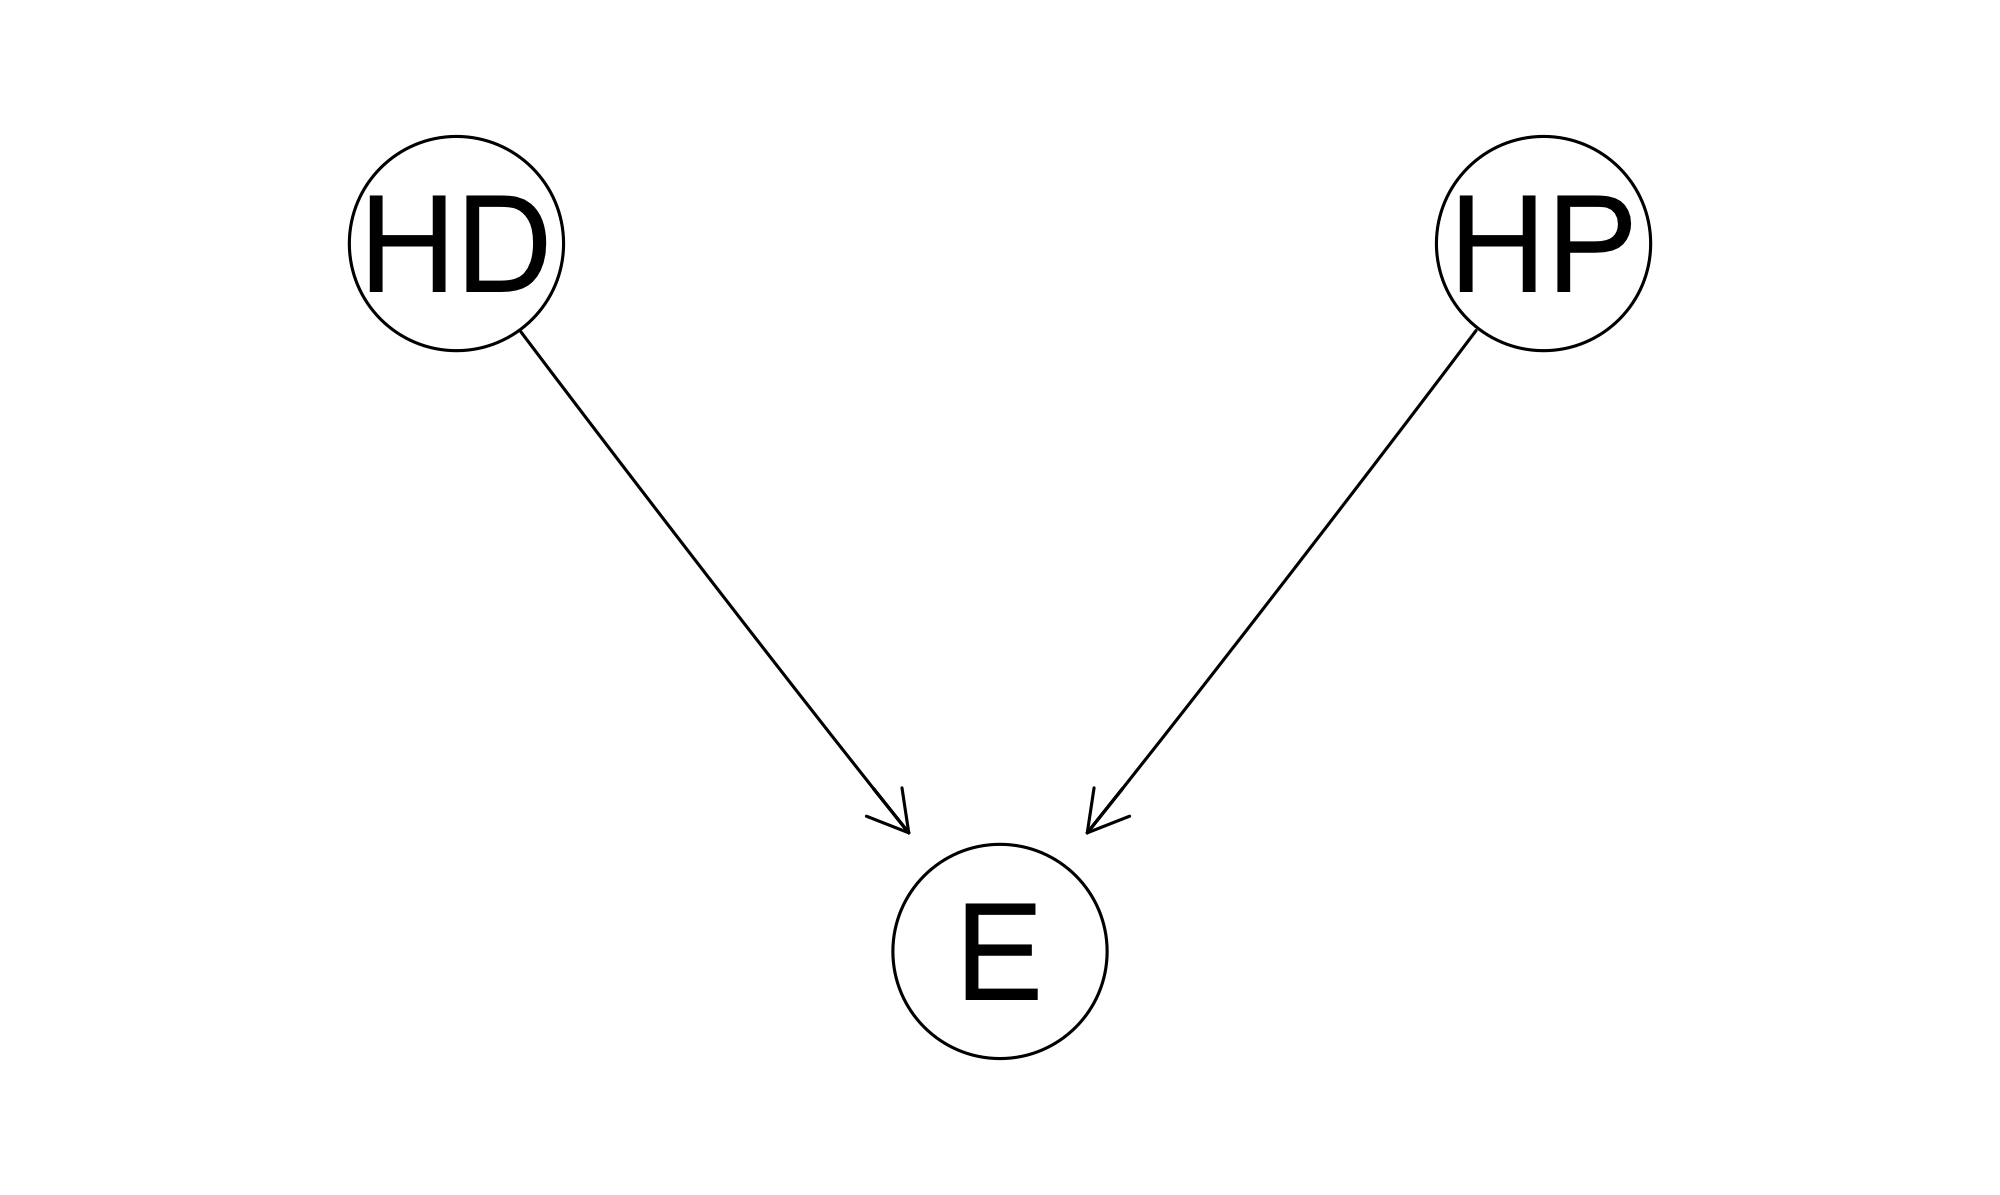
\includegraphics[scale = 0.08]{STMdag.png}}
%		{\caption{\footnotesize Graphic model of Small Town Murder}\label{fig:bayes_test4}}
%		\ffigbox{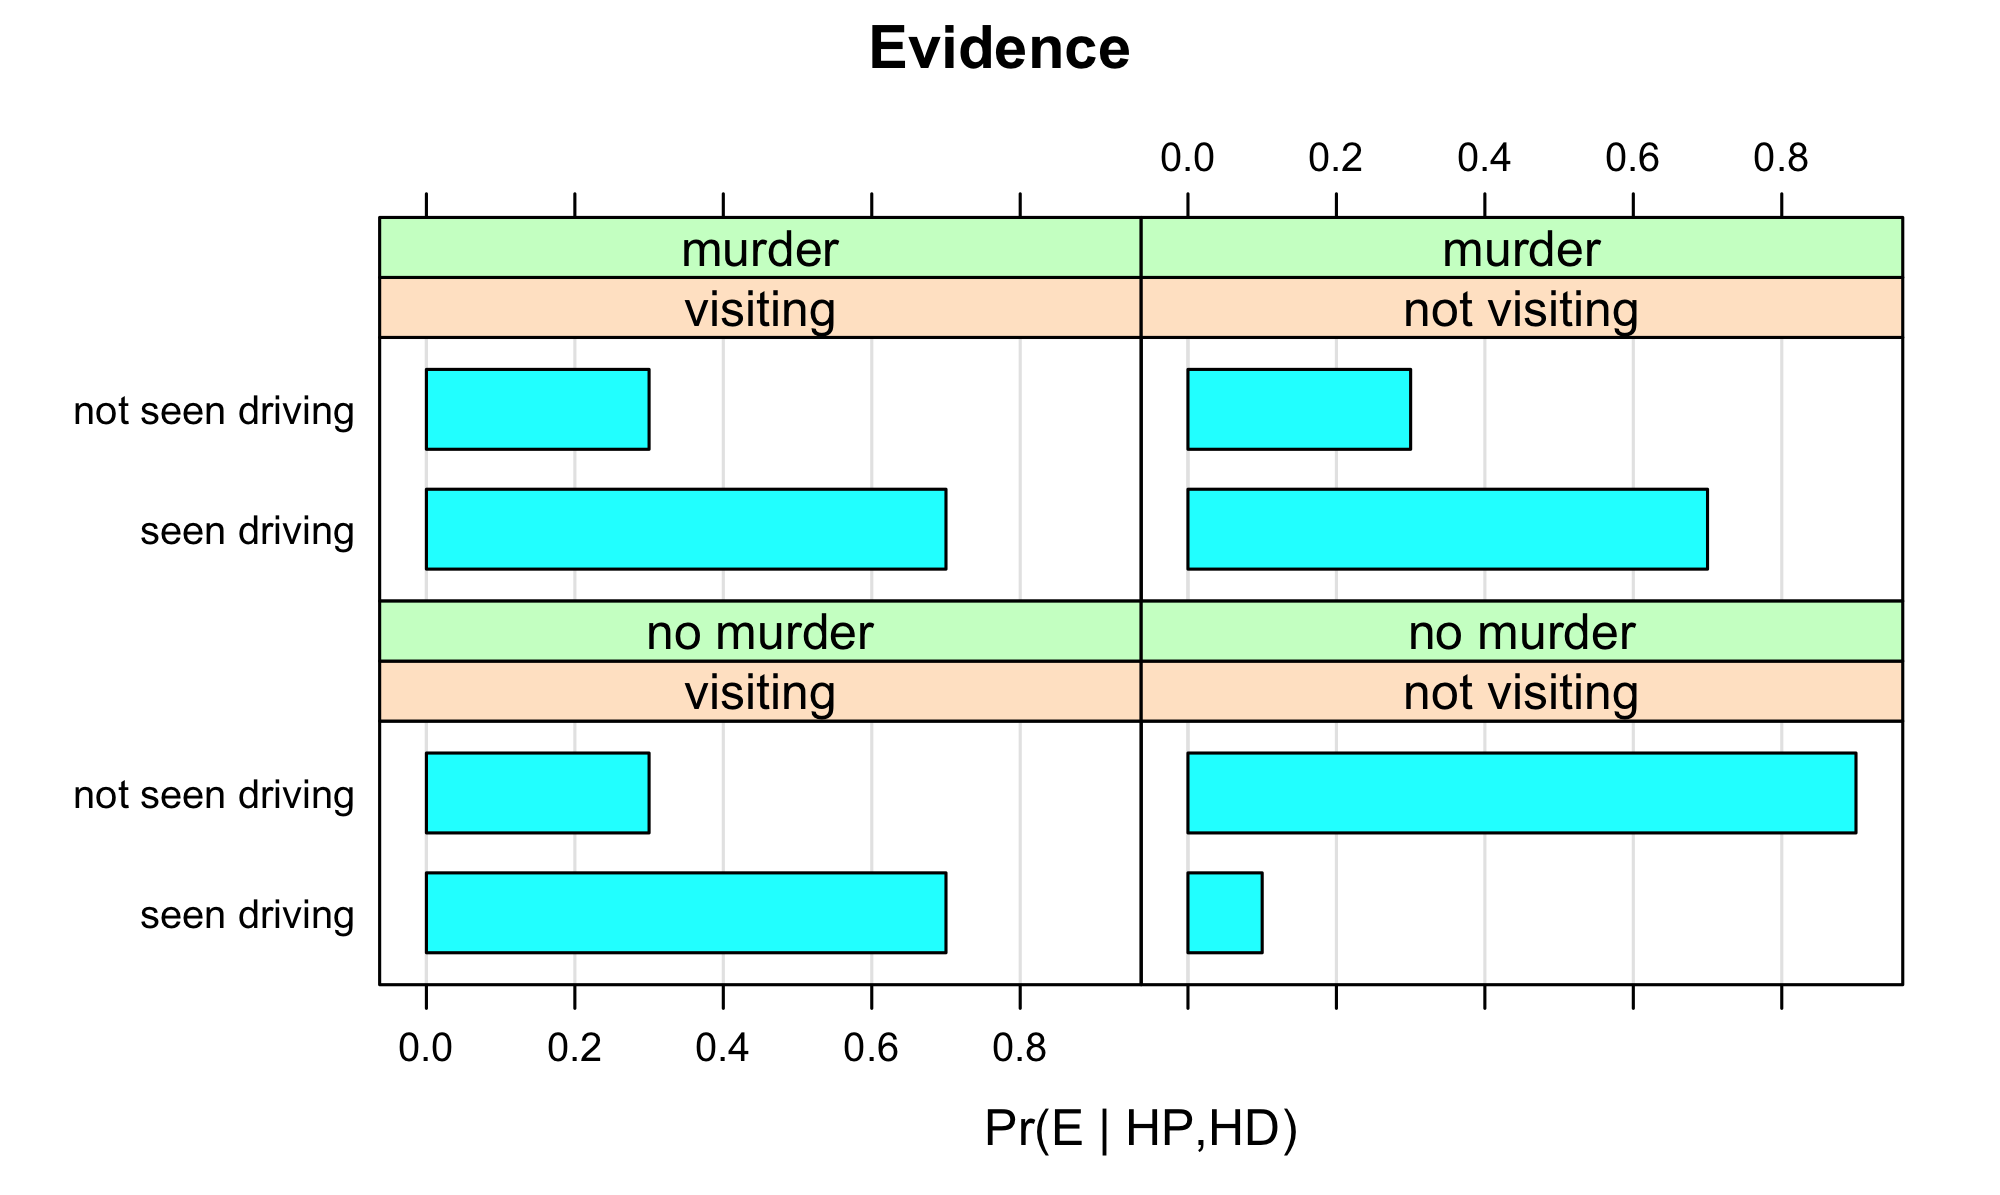
\includegraphics[scale = 0.08]{STMpt.png}}{
%			\caption{\footnotesize Probability distribution of $E$}\label{fig:bayes_test6}}
%	\end{floatrow}
%\end{figure}
%

\noindent
  %Following the calculations in \citep{dezoete2019ResolvingSocalledProbabilistic}, for exclusive and exhaustive hypotheses, $LR(E,H_d,\neg H_d)=1.75$, and similarly, $LR(E,H_p, \neg H_p)=1.75$, since $P(E\vert H_d)=0.7$ and $P(E\vert \neg H_d)=0.4$. 
  %The likelihood ratio of the evidence, if it is measured against exclusive and exhaustive hypotheses, is not equal to one.\footnote{ \cite{dezoete2019ResolvingSocalledProbabilistic} offer a slightly different solution to the problem. They construct a Bayesian network with three hypotheses, also exhaustive and exclusive: in town to visit mother, in town to murder, out of town.} 
%Such considerations should also generalize to other paradoxes of relevance.  
%
%For instance,  in the twins problem, the LR is 1 if the hypotheses are: `the suspect committed the crime', and `the suspect's twin brother committed the crime', but is not 1 f we consider the fairly natural hypothesis that  the defendant is  innocent. 
%Similarly, 
%In the food tray example, Bayesian network analysis shows that the value of the evidence `prisoner withholds tray' for the question who started the fight depends on a range of uncertain events and other pieces of evidence (such as whether indeed a parcel he was supposed to obtain was withheld;  whether the prisoner inquired about this; whether and how this inquiry was answered). Considered in this context, the piece of evidence will not have a likelihood ratio of one with respect to at least some choice of sensible hypotheses.
%

The problem with the  paradoxes of relevance is that in complex situations there is no single likelihood ratio that corresponds to a piece of evidence. The problematic cases focus on a single likelihood ratio based on non-exclusive or non-exhaustive hypotheses.  However, evidence can be relevant so long as it has a probabilistic impact on a  pertinent sub-hypothesis,  even without having a probabilistic impact on the prosecutor's or defense's ultimate hypotheses. When this happens, the evidence is relevant, in agreement with Rule 401 of the Federal Rules of Evidence. Bayesian networks (discussed in the preceding section) help to see how pieces of evidence can increase or decrease the probability of different sub-hypotheses  \citep[for more details, see][]{dezoete2019ResolvingSocalledProbabilistic}. 


%recommend relying on a Bayesian network to investigate in an orderly manner the way in which pieces of evidence and hypotheses interact.\todo{no one said the interact in an orderly manner. ;) } %in an orderly manner.   














\section{Standards of proof}
\label{sec:burden}

After the evidence has been presented, examined and cross-examined at trial,  trained judges or lay jurors must reach a decision \citep[see][for a few caveats on what the decision should be about]{Laudan2010verdicts}.
%
%Trial decisions should of course be based on the evidence, not on prejudice or subjective conviction. But
%How strong should the evidence against the defendant be to warrant a judgment of civil or criminal liability? 
The decision criterion is defined by law 
and consists of a standard of proof, also called the burden of persuasion. 
If the evidence against the defendant is sufficiently strong to meet the requisite proof standard, the defendant should be found liable. This section begins with a description of standards of proof in the law, then outlines a probabilistic account of standards of proof, and finally discusses some objections to this account. 



\subsection{Legal background}
\label{subsec:legal-background}

 %There may be some variability about  the standards to be applied. 
 
In criminal proceedings, the governing standard is `proof beyond a reasonable doubt.' In civil cases, the standard is typically `preponderance of the evidence.' The latter is less demanding than the former, so the same body of evidence may be enough to meet the preponderance standard, but not enough to meet the beyond a reasonable doubt standard. A vivid example of this difference is the 1995 trial of O.J. Simpson who was charged with murdering his wife. He was acquitted of the criminal charges, but when the family of the victim brought a lawsuit against him, they prevailed. O.J.\ Simpson did not kill his wife according to the beyond a reasonable doubt standard, but he did according to the preponderance standard. An intermediate standard, called `clear and convincing evidence', is sometimes used for civil proceedings in which the decision is particularly weighty, for example, a decision whether someone should be involuntarily committed to a hospital facility. 

%This tripartite distinction of proof standards---beyond a reasonable doubt; preponderance; clear and convincing evidence---is common in Anglo-american jurisprudence. It is not universal, however. %Different countries may use different standards. 
%France, for example, uses the standard of `intimate conviction' for both civil and criminal proceedings. Judges deciding cases `must search their conscience in good
%faith and silently and thoughtfully ask themselves what impression the evidence
%given against the accused and the defence's arguments have made upon them' (French Code of Criminal Procedure, art.\ 353). %German law is similar. 
%Along similar lines, Germany's Code of Civil Procedure, Sec.\ 286, states that `it is for the court to decide, based on its personal conviction, whether a factual claim is indeed true or not.'
%In criminal cases, if the decision makers are persuaded beyond a reasonable doubt that the defendant is guilty, they should convict, or else they should acquit. 
%Proof standards impose different evidential requirements in different cases. 
%The standard `proof beyond a reasonable doubt' in criminal cases is more stringent than `preponderance of the evidence' in civil cases. But no matter how stringent, no proof standard will ever require certainty.
%In Commonwealth v.\ Massachusetts Webster (1850), %proof beyond a reasonable doubt is equated to `reasonable and moral certainty.' 
%
%


How to define standards of proof, or whether they should be even defined in the first place, remains  contentious \citep{diamond90,newman1993, Horowitz1996,laudan2006truth,walen2015}. Judicial opinions offer different paraphrases, sometimes conflicting, of what these standards mean. The meaning of `proof beyond a reasonable doubt' is the most controversial. It has been equated to `moral certainty' or `abiding conviction' (Commonwealth v. Webster, 59 Mass. 295, 320 (1850)), or to `proof of such a convincing character that a reasonable person would not hesitate to rely and act upon it in the most important of his own affairs' (US Federal Jury Practice and Instructions, 12.10, at 354, 4th ed.\ 1987). But courts have also cautioned that there is no need to define the term because `jurors know what is reasonable and are quite familiar with the meaning of doubt' and attempts to define it only `muddy the water' (U.S. v. Glass, 846 F.2d 386, 1988).

Probability theory can bring conceptual clarity 
to an otherwise heterogeneous legal doctrine, 
or at least this is the position of legal probabilists.

\subsection{Probability thresholds}

%\todo{M: talk about thresholds. DONE SEE BELOW FINAL PARAGRAPH. } 

Legal probabilists have proposed to interpret proof beyond a reasonable 
doubt as the requirement that the defendant's probability of guilt, given the evidence presented at trial, meet a threshold, say, $>$.95. Variations of this view are common  \citep[see, for exmaple,][]{Bernoulli1713Ars-conjectandi, Laplace1814,  kaplan1968decision, Dekay1996, kaye79, laudan2006truth}. This interpretation is, in some respects, plausible. %In experimental research, the probabilistic interpretation 
%is taken for granted in  studies about people's understanding of proof beyond a reasonable doubt \citep{dhamiEtAl2015}. 
%This research examines whether
%people use a 75\% or 95\% threshold, but does not question whether the standard functions as a probabilistic threshold.
From a legal standpoint, the requirement that guilt be established with high probability, still short of 1, accords with the  principle that proof beyond a reasonable doubt is the most stringent standard of all but %at the same time 
`does not involve proof to an absolute certainty' and thus `it is not proof beyond any doubt' (R v Lifchus, 1997, 3 SCR 320, 335).



Reliance on probabilistic ideas is even more explicit in the standard `preponderance of the evidence'---also called `balance of probabilities'---which governs decisions in civil disputes. This standard can be interpreted as the requirement that the plaintiff---the party making the complaint against the defendant---establish its version of the facts with greater than probability of .5. The .5 threshold, as opposed to a more stringent threshold of .95 for criminal cases, reflects the fact that  preponderance is less demanding than proof beyond a reasonable doubt. The intermediate standard `clear and convincing evidence' is more stringent than the preponderance standard but not as stringent as the beyond a reasonable doubt standard. Since it lies in between the other two, it can be interpreted as the requirement that the plaintiff establish its versions of the facts with, say, probability at the level of .75-.8.

Some worry that a mechanical application of numerical thresholds would undermine the humanizing function of trial decision-making. %Decision makers, guided by the seemingly inexorability of numbers, may forget their humanizing  function. 
As \cite{tribe71} put it, `induced by the persuasive force of formulas and the precision of  decimal  points  to  perceive  themselves  as  performing  a  largely mechanical and automatic  role, few jurors \dots could be relied upon to recall, let alone to perform, [their] humanizing function.' 
%Legal probabilists  will concede that a mechanical applications of probability thresholds may have unintended effects on the psychology of jury decision-making. 
Thresholds, however, can vary depending on the costs and benefits at stake in each case (see later discussion). So they need not be applied mechanically without considering the individual circumstances  \citep{HeddenColyvan2019legal}. Furthermore, if jurors are numerically literate, they should not lose sight of their humanizing function as they would no longer be intimated by numbers. So the worry suggests the need to ensure that jurors are numerically literate, not dispensing with probabilistic thresholds altogether. 


Even if numerical thresholds cannot be used in the daily business of trial proceedings, they
can still serve as theoretical concepts for understanding the role of proof standards in the justice system, such as regulating the relative frequency of false positive and false negative decisions or minimizing expected costs.
%Proof standards can be viewed as instruments to regulate the long-run frequency of false positives (say, false convictions) and false negatives (say, false acquittals). 
%If the standard is made more stringent, fewer people will be found liable, and 
%In criminal cases, this means that fewer innocent people will be convicted (resulting in fewer false convictions) and fewer guilty people will be convicted (resulting in more false acquittals).
%conversely, if the standard is made less stringent, more people will be found liable. 
%In criminal cases, this means that more innocent people will be convicted (resulting in more false convictions) and more guilty people will be convicted (resulting in fewer false acquittals). 
A more stringent threshold will decrease the number of false positives (say false convictions) at the cost of increasing the number of false negatives (say false acquittals), and a less stringent threshold will increase the number of false positives while decreasing the number of false negatives.
This trade-off has been described, among others, by Justice Harlan in his concurring opinion in re Winship, 397 U.S. 358, 397 (1970).  
%Against this background, it is natural to ask what the optimal or most efficient threshold should be. The optimal threshold may be one that minimizes false positives and false negatives overall or one that minimizes expected costs. Which threshold would minimize overall errors? Which would minimize expected costs?
%The decision threshold that minimizes errors overall happens to be $>50\%$ (see below for a proof). If, however, one type of error is  more costly than the other---for example, a false conviction is regarded as more harmful than a false acquittal---a more stringent threshold, say $>90\%$, should be preferable. These 
%conclusions are intuitively plausible, but 
As shown below, the formal apparatus of probability theory, in combination with expected utility theory, can make this point more precise. 



\subsection{Minimizing expected costs}

%Instead of thinking in terms of false positives and false negatives, probabilistic can also be viewed through the lenses of expected utility theory  

  Expected utility theory recommends agents to take the course of action that, among the available alternatives,  maximizes expected utility. On this view, 
the standard of proof is met whenever the expected utility (or cost) of a decision against the defendant (say, a conviction) is greater (or lower) than the expected utility (or cost) of a decision in favor of the defendant (say, an acquittal) \citep{kaplan1968decision, Dekay1996, hamer2004}.
Let $c(CI)$ be the cost of convicting a factually innocent defendant and $c(AG)$ the cost of acquitting a factually guilty defendant. For a conviction to be justified, the expected cost of convicting an innocent---that is, $c(CI)$  discounted by the probability of innocence $[1-\Pr(G|E)]$---must be lower than the expected cost of acquitting a guilty defendant---that is, $c(AG)$ discounted by the probability of guilt $\Pr(G|E)$. This holds just in case 
%
\[ \frac{\Pr(G|E)}{1- \Pr(G|E)} > \frac{c(CI)}{c(AG)}.\]
%
This inequality captures 
how high the probability 
of guilt or civil liability must be to justify a verdict against the defendant. 
When the cost ratio $\frac{c(CI)}{c(AG)}$ is set to 9---which might be appropriate in a criminal 
case since convicting an innocent is often considered more harmful than acquitting a guilty defendant \citep[however, see ][]{laudan2016law} ---the inequality holds only if $\Pr(G | E)$ meets the .9 threshold.
%
The same analysis \textit{mutatis mutandis} applies to civil cases in which mistaken decisions comprise mistaken attributions of liability (false positives) and mistaken failures to attribute liability (false negatives). If the cost ratio is one---as might be appropriate in a civil case in which false positives and false negatives are equally harmful---the inequality holds only if the probability that the defendant is liable meets the .5 threshold. %Interestingly, this analysis based on the minimization of expected costs arrives at the same conclusion as the previous analysis based on the minimization of error rates. 


%
%Since the costs ratio is different in civil and criminal cases, the threshold probability in different as expected.
%


\begin{center}
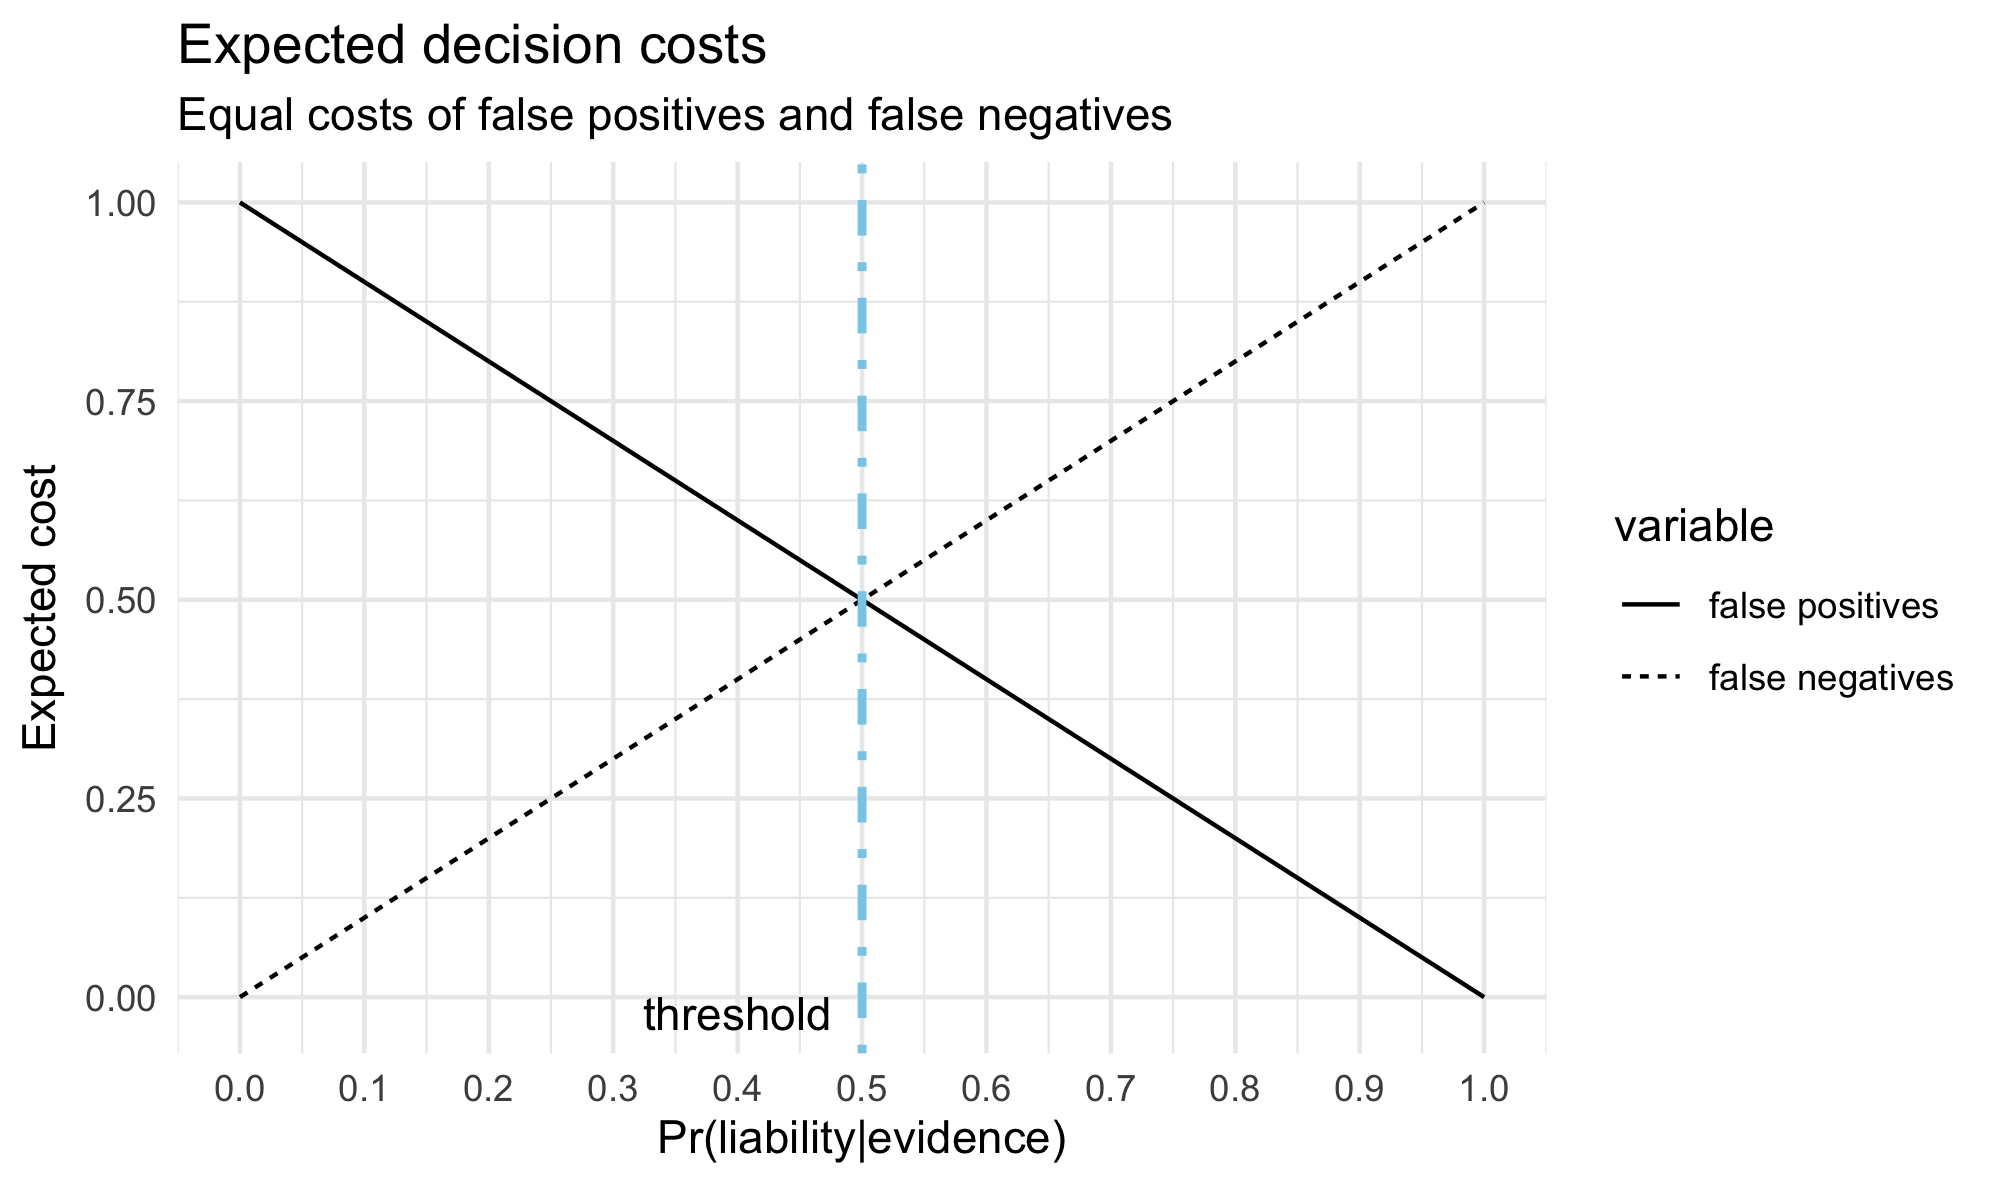
\includegraphics[width=10cm]{civil2.png}
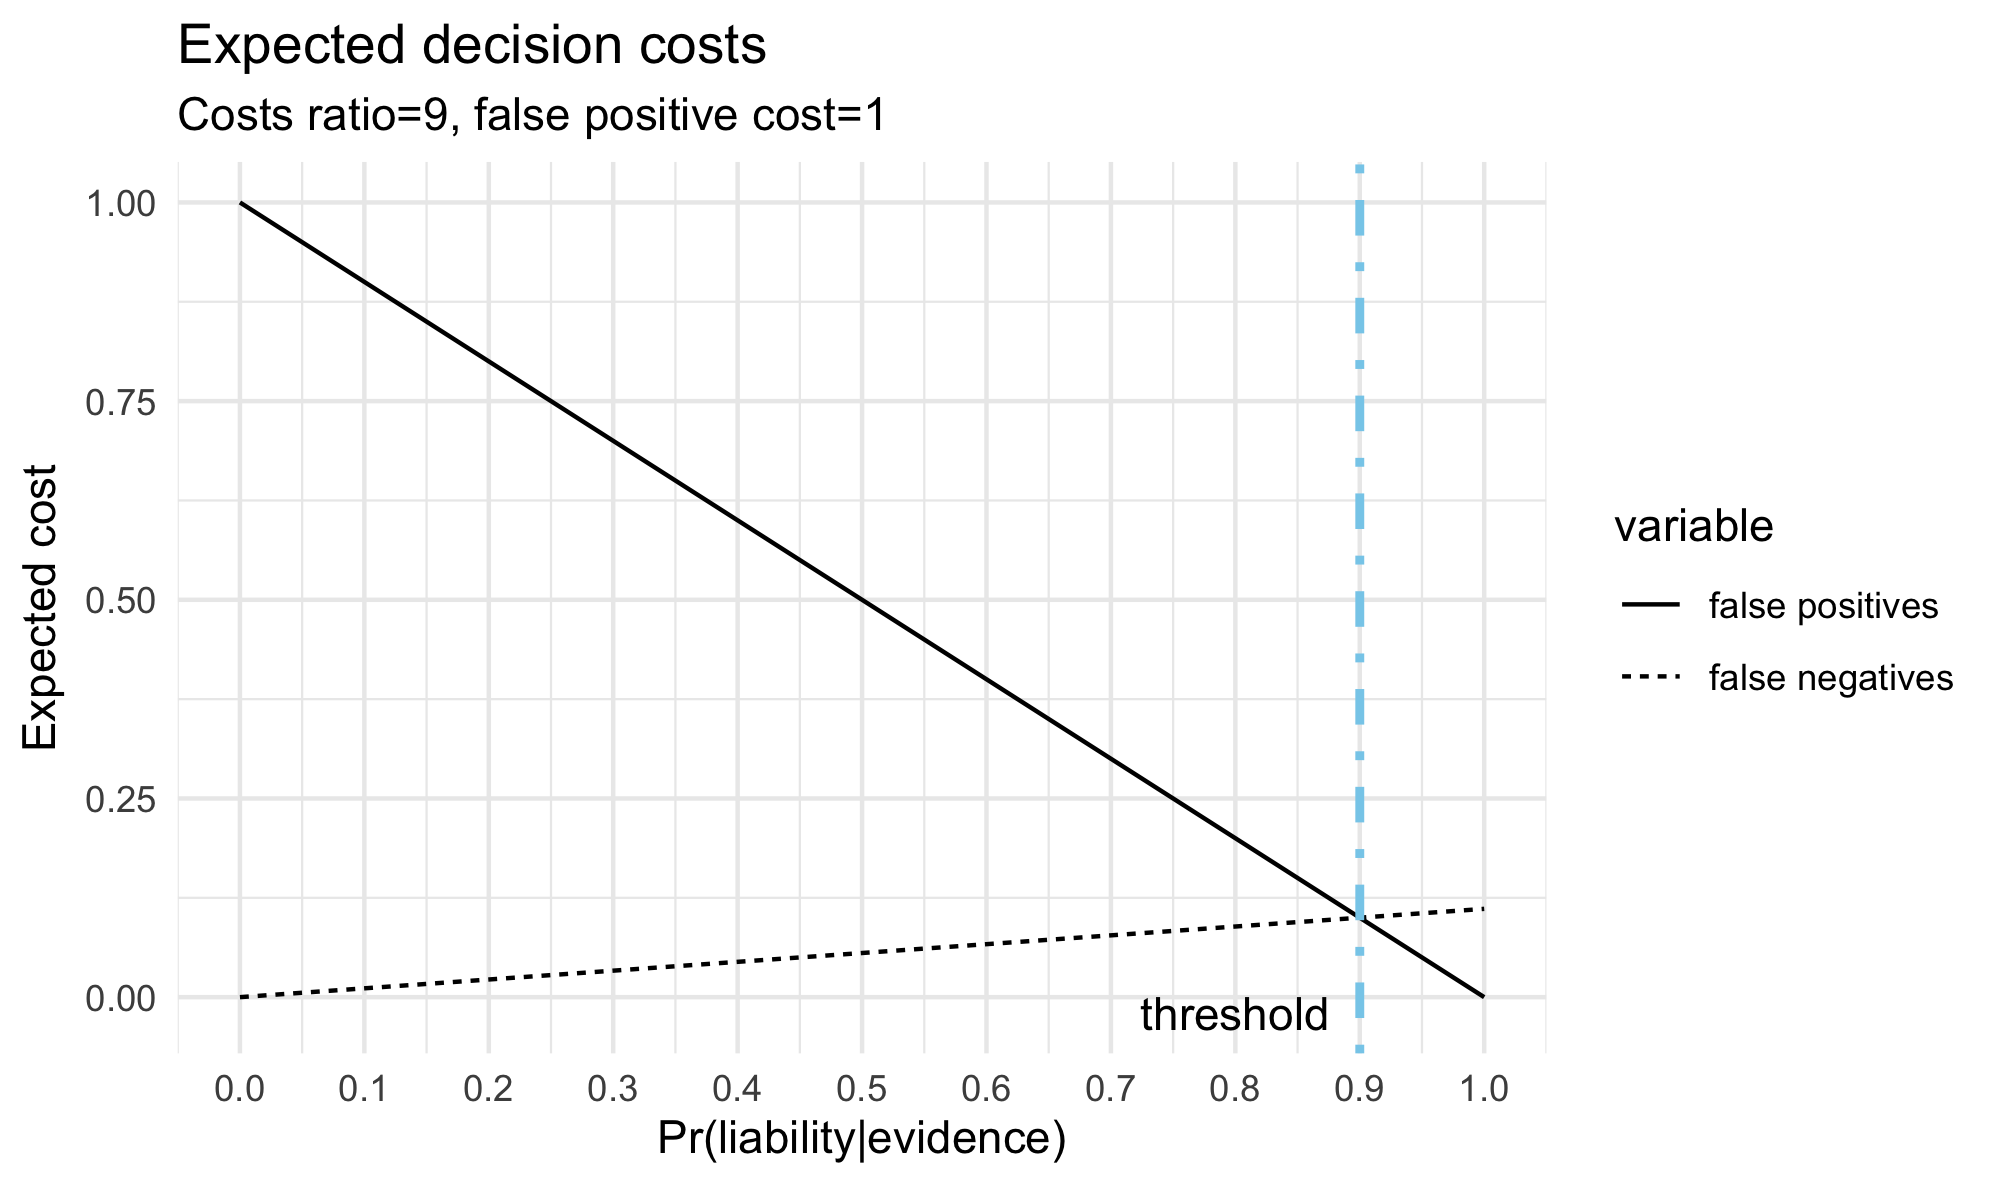
\includegraphics[width=10cm]{criminal4.png}   
\end{center}


% \begin{figure}[h!] 
%  \centering
% \begin{tikzpicture}
% \begin{axis}[
%   no markers, domain=0:1, samples=100,
%   axis lines*=left, xlabel=\textsc{\tiny $Pr(\text{Liability} | \text{Evidence})$}, ylabel=\textsc{\tiny expected cost},
%   legend pos=north west,
%   height=5cm, width=6.5cm,
%   xtick={0.5, 1}, 
%  %ytick={0, 0.2, 0.4},
%   xticklabels={\tiny{0.5},
%   \tiny{1}},
%  % yticklabels={0, 0.2, 0.4, 0.6},
%     enlargelimits=false, clip=false, axis on top,
%   grid = major
%   ]
%   \addplot  [black] {x*0.5} \closedcycle;
%     \addplot  [dashed] {(1-x)*0.5} \closedcycle;
%     % \legend{\tiny{}, \tiny{} } ; 
% \end{axis}
% \end{tikzpicture}
% %
% \begin{tikzpicture}
% \begin{axis}[
%   no markers, domain=0:1, samples=100,
%   axis lines*=left, xlabel=\textsc{\tiny $Pr(\text{Guilt} | \text{Evidence})$}, ylabel=\textsc{\tiny },
%   legend pos=north west,
%   height=5cm, width=6.5cm,
%   xtick={ 0.90, 1}, 
%  %ytick={0, 0.2, 0.4},
%   xticklabels={
%   \tiny{0.9}, \tiny{1}},
%  % yticklabels={0, 0.2, 0.4, 0.6},
%     enlargelimits=false, clip=false, axis on top,
%   grid = major
%   ]
%   \addplot  [black] {x*0.1} \closedcycle;
%     \addplot  [dashed] {(1-x)*0.9} \closedcycle;
%     % \legend{\tiny{expected cost of a false acquittal}, \tiny{expected cost of false conviction} } ; 
% \end{axis}
% \end{tikzpicture}
% %


%In civil cases, the expected cost of a false negative  exceeds the expected cost of a false negative as soon as the probability of liability reaches 50\%. In criminal cases, instead, the expected cost of a false negative exceeds the expected cost of a false negative  when the probability of guilt reaches 90\%. 


This analysis only considers the costs of mistaken decisions, but leaves out the benefits associated with correct decisions. More comprehensive analyses would consider both, but the basic insight would remain the same. Trial decision-making is viewed as one instrument among others  for maximizing overall social welfare \citep{Posner1973}. 
%The probability required for a conviction or a finding of civil liability against the defendant is a function of weighing the  costs and benefits that would result from true and false positive as well as true and false negative decisions. 
On this account of proof standards, the stringency of the threshold depends on costs and benefits, and thus different cases may require different thresholds. Cases in which the charge is more serious than others---say, murder compared to petty theft---may require higher thresholds so long as the cost of a mistaken decision against the defendant is more significant. %Standards of proof would vary depending on the costs at stake in different cases.
Whether or not standards of proof should vary in this way is debated \citep{kaplow2012, picinali2013}.








 %The same standard of proof is typically applied for murder and petty theft.
 %The law typically  makes coarse  distinctions between standards of proof, such as `proof beyond a reasonable doubt' for criminal cases, `preponderance of the evidence' for civil cases and `clear and convincing evidence' for a narrow subset of civil cases in which the accusation against the defendant is particularly serious.
 %Another complication is that eliciting costs and benefits that result from trial decisions is not easy.  Should they be elicited through a democratic process or should different jurors or judges apply their own in a subjective fashion? 
 %(CITE WHAT?)
%No matter the answer to these questions, when probabilistic standards of proof are paired with expected utility theory, they become part of the calculus of utilities. 


%\todo{M: note to
%self. Add brief mention of Biederman's work on expected utility theory in forensic reporting.}


%\subsection{Minimizing overall errors}


%Consider an idealized model of the criminal trial system.  Each defendant is assigned a probability $x$ of criminal liability (or guilt) based on the evidence presented at trial. 
%As is standard, this probability ranges between 0 and 1, or 0\% and 100\%. 
%Since over a period of time many defendants face charges, the guilt probability will have its own distribution.  Extreme guilty probabilities set at 0\% or 100\%, presumably,  are assigned rarely in trials if ever, while values between 40\% and 80\% are more common.  
%A rigorous way to express this distribution is by means of a probability density function, call it  $f(x)$.  
%Similarly, the probability of non-liability $1-x$ has its own probability density function $f(1-x)$.
%The figure below uses a right skewed
% distribution $\textsf{beta(18,3)}$. 



%Beta density  distributions are often used to represent priors in Bayesian context. Think of it as representing uncertainty about the bias of a coin after seeing 18 heads in 21 tosses. For the sake of example, suppose we fix conviction threshold at $.8$ and are additionally interested in the (shaded) area for $x\in (.8,.9)$. The distribution looks like this.

%\begin{center}
%    \includegraphics[width=10cm]{bet%a(18,3)2.png}
%\end{center}
 
% \noindent
 %The right skew reflects the assumption that defendants in criminal cases are sent to trial only if the incriminating evidence against them is strong. It should be no surprise that most defendants are assigned a high probability of guilt. The distribution of the probability of liability in civil cases over a period of time might look quite different, probably centered around 50\% or 60\%.
 

%, that is, $\int_0^1 \! f(x) \, \mathrm{d}x=1$.
%In the figure above, the threshold for conviction is set at $>80\%$, and the area under the curve to the right of the threshold is about $.79$. 
%In other words, according to this model, 79\% of defendants on trial are convicted and 21\% acquitted. These figures are close to the rates of conviction and acquittal in many countries. 
%Since $f(x)$ is a probability density, the total area under the curve adds up to 1, encompassing all defendants, both convicted and acquitted defendants. 
%
%If the threshold becomes more stringent---for example, it moves up to 85\%---the rate of conviction would decrease provided the underlying distribution does not change. But if the distribution becomes more skewed toward the right---say \textsf{beta(25,3)}---the rate of conviction could still be about 79\% even with a more stringent threshold of 85\%. 

%\begin{center}
%    \includegraphics[width=10cm]{dbe%ta(25,3)2.png}
%\end{center}


%The shaded area---between guilt probability 80\% and 90\%---equals 47\%, that is, about 47\% of the defendants are assigned a guilt probability between 80\% and 90\%.  In integral form, $\int_{0.8}^{0.9} \! f(x) \, \mathrm{d}x=0.47$. 
%Suppose  1000 people face trial. If the guilt probability distribution was \textsf{beta(18,3)} and  the frequencies matched the probabilities, this would mean  470 people would be assigned guilt probability between $.8$ and $.9$ by the court, and that 790 of all the defendants would be convicted. 
 
% This formal model can also distinguish between innocent and guilty defendants.  
%The expected proportion of guilty and innocent defendants on trial, out of all defendants, can be inferred from the density distribution $f(x)$ under certain assumptions. Suppose each defendant is assigned a guilt probability based on the best and most complete evidence. 
   %  assigned by the court as our best estimate of guilt probability (it definitely should be the best one from the perspective of the court!). Then, out of the 470 people assigned guilt probability between $.8$ and $.9$, the court should believe that fewer, between $.8\times 470 = 376$ and $.9\times 470=423$ actually will be guilty. 
%  To a good approximation,
%\todo{I don't think we have to assume this is good approximation; we don't know; all we know is that this is what court thinks}
%From the perspective of judges and jurors (or anyone who has access to the evidence and evaluates it the same way), 
%$x\%$ of defendants who are assigned  $x\%$ guilt probability are expected to be guilty and $(1-x)\%$ innocent. For example, 85\% of defendants  who are assigned a 85\% guilt probability are expected to be guilty and 15\% innocent.
%; 90\% of defendants  who are assigned a 90\% guilt probability are expected to be guilty and 10\% innocent; and so on.  
  %.85 assigned, 85\% would be expected to be guilty, etc. Once we calculate this properly, out of 1000 defendants, around $.4$ (400 defendants),  are expected to be assigned guilt probability $x\in (.8, .9)$ and be guilty. Generally, out of people with assigned guilt probability $f(x)$, $100x\%$ is expected to be actually guilty, and 
  %So the distribution of expected actual guilt distribution as a function of $x$ will be $x f(x)$. 
%Consequently, the function $xf(x)$ describes the (expected) assignment  of guilt probabilities for guilty defendants, and similarly, $(1-x)f(x)$   the (expected) assignment of guilt probabilities for innocent defendants. Neither of these functions is a probability density, since %$\int_0^1 \! xf(x) \, \mathrm{d}x=0.86$ and $\int_0^1 \! (1-x)f(x) \, \mathrm{d}x=0.14$. %That is, 
%the total areas under the curve are, respectively, $.86$ and $.14$ (see graphs below).
% These numbers express the (expected) proportion of guilty and innocent defendants out of all defendants on trial, respectively 86\% and 14\%. 
 
%The rates of incorrect decisions---false convictions and false acquittals or more generally false positives and false negatives---can be inferred from this model as a function of the threshold $t$ \citep{hamer2004, hamer2014}. The integral $\int_0^t \! xf(x) \, \mathrm{d}x$ equals the expected rate of false acquittals, or in other words, the expected proportion of guilty defendants who fall below threshold $t$ (out of all  defendants), and the  integral $\int_t^1 \! (1-x)f(x) \, \mathrm{d}x$ equals the expected rate of false convictions, or in other words, the expected proportion of innocent defendants who fall above threshold $t$ (out of all defendants).
%The rates of correct decisions---true convictions and true acquittals or more generally true positives and true negatives---can be inferred in a similar manner. The integral $\int_t^1 \! xf(x) \, \mathrm{d}x$ equals the expected rate of true convictions and $\int_0^t \! (1-x)f(x) \, \mathrm{d}x$ the expected rate of true acquittals. In the figure below, the regions shaded in gray correspond to false negatives (false acquittals) and false positives (false convictions).
%The remaining white regions within the solid black curve correspond to true positives (true convictions) and true negatives (true acquittals). Note that the dotted blue curve is the original overall distribution for all defendants. 

 %This is what the assignments of the guilt probability $x$ for guilty and innocent defendants look like (the blue curve is the original overall distribution for all defendants):



 %\begin{center}
 %   \includegraphics[width=10cm]{xfx% 3.png}
%\end{center}



%\begin{center}
 %   \includegraphics[width=10cm]{nxf% x3.png}
%\end{center}




%\todo{not sure the title "expectation for the innocent" or "expectation for the guilty" is ideal. Does this refer to the curve or the integrals? Maybe "innocent distribution" and "guilty distribution"?}

%\todo{Emphatically, these are not distributions because they don't integrate to 1. I changed the titles a bit, are they ok now?}
 
%\todo{Is the blue line ok now?}
 
% This is not a probability density distribution, because the total area under the curve is around .86, not 1. Rather, the integrals (areas under the curve) correspond to the proportions of the \emph{original population of defendants} who are expected to be both guilty and be assigned a given probability of guilt. Since the expected guilty people are all the guilty people assigned some guilt probability, the integral
%# $\int_0^1 \! xf(x) \, \mathrm{d}x$ is the expected value of $x$, that is, the expected probability of guilt assigned to the defendants in general.

%Continuing our numerical example, since if $\int_0^1 \! xf(x) \, \mathrm{d}x\approx.86$, the court expects $860$ people to be guilty in total, irrespective of what guilt probability they will be assigned.


%Similarly, $(1-x)f(x)$  describes the expected assignment of guilt probabilities to innocent defendants. For instance, among those assigned probability of guilt .8 the court should expect $100(1-.8).8\%=16\%$ to be innocent. Continuing our example, $470$ will be assigned $x\in(.8,.9)$, and $100\int_{.8}^{.9}xf(x)\, \mathrm{d}x\approx .07\%$ of the defendants (not of the innocent!), that is $0.07\times 1000=70$ are expected to be innocent. This adds up. 470 are expected to be assigned probability of guilt in $(.8,.9)$, 400 of them are expected to be guilty, and 70 are expected to be innocent. Notice $\int_0^1 \! (1-x)f(x) \, \mathrm{d}x\approx .14$, so out of 1000 defendants, 140 are expected to be innocent, no matter what guilt probability is assigned to them.



%The size of the grey regions in the figures above---which correspond to false positives and false negatives---is affected by the location of threshold $t$. As $t$ moves upwards, the rate of false positives decreases but the rate of false negatives increases. Conversely, as $t$ moves downwards, the rate of false positives increases but the rate of false negatives decreases. This trade-off is inescapable so long as the underlying distribution is fixed. Below are both error rates---false positives and false negatives---and their sum plotted against a choice of $t$, while holding fixed the   density function $\textsf{binom(18,3)}$.
%The graph shows that any threshold that is no greater than 50\% would minimize the total error rate %(comprising false positives and false negatives). 
%A more stringent threshold, say $>90\%$, would instead  significantly reduce the rate of false positives but also significantly increase the rate of false negatives, es expected. 

%\begin{center}
 %   \includegraphics[width=12cm]{err% ors.png}
%\end{center}
 

 
% Suppose  1000 people face trial, and $f(x)$ is such that the area under the density curve going\todo{Actually, I meant the area under the curve, fixed.} from  $f(81)$ to $f(80)$  is $.8$. This would mean that if the frequencies matched the probabilities, 800 people would be assigned guilt probability between $.80$ and $.81$ by the court.
 
% Now imagine we take the probability assigned by the court as our best estimate of guilt probability (it definitely should be the best one from the perspective of the court!). Then, out of the 800 people assigned guilt probability between $.8$ and $.81$, we should believe actually $80-81\%$, that is, between $.8\times 800$ and   $.81 \times 800=640-648$ are guilty.  Similarly, out of 800 people assigned guilt probability in $(.8,.81)$, between $.19\times 800=152$ and $.2\times 800 = 150$ the court expects to be innocent. For this reason $xf(x)$ ($(1-x)f(x)$) represents court's density distribution of guilty (innocent) people who are assigned guilt probability $x$. \todo{Now I like what you did to clarify this!}
 
 %Since the guilty people are all the guilty people assigned some guilt probability, the integral
%$\int_0^1 \! xf(x) \, \mathrm{d}x$ is the expected value of $x$, that is, the expected probability of guilt assigned to the defendants in general. So, continuing our numerical example, if $\int_0^1 \! xf(x) \, \mathrm{d}x=0.9$ the court expects $.9\times 800$ people to be guilty, irrespective of what guilt probability they will be assigned.   Similarly, $\int_0^1 \! (1-x)f(x) \, \mathrm{d}x$ is the expected probability of being innocent (in our example: the court expects 80 people to be innocent, without any assumption on  what guilt probability they will be assigned).  

%Now suppose the decision criterion is a threshold  $t$. $\int_0^t \! xf(x) \, \mathrm{d}x$ is the court's expected frequency of guilty people who would fall below $t$, that is the expected frequency of  false negatives. Similarly, $\int_t^1 \! (1-x)f(x) \, \mathrm{d}x$ is the court's expected frequency of  false positives.

%As $t$ moves upwards, the number of false positives decreases and the number of false negatives increases. As $t$ moves downwards, the number of false positives increases and the number of false negatives decreases.
 
 
 
 
%\begin{comment}
%\begin{figure}[h!]
%\begin{tikzpicture}
%\begin{axis}[
%  no markers, domain=0:1, samples=1000,
%  axis lines*=left, xlabel=\textsf{}, ylabel=\textsf{$x f(x)$},
%  height=5cm, width=6cm,
%  xtick={0, 0.80, 1}, ytick=\empty,
%  xticklabels={0, t, 1},
%  enlargelimits=false, clip=false, axis on top,
%  grid = major
%  ]
 %   \addplot [fill=blue!60, draw=none, domain=0:0.8] {x*(x^2*(1-x)*5)} \closedcycle;

 %  \addplot  [red]{x*(x^2*(1-x)*5)}; % 
%\end{axis}
%\end{tikzpicture}
%\hspace{12mm}
%\begin{tikzpicture}
%\end{tikzpicture}
%\begin{tikzpicture}
%\begin{axis}[
%  no markers, domain=0:1, samples=1000,
%  axis lines*=left, xlabel=\textsf{}, ylabel=\textsf{$(1-x) f(x)$},
%  height=5cm, width=6cm,
%  xtick={0, 0.80, 1}, ytick=\empty,
%  xticklabels={0, t, 1},
%  enlargelimits=false, clip=false, axis on top,
%  grid = major
%  ]
%  \addplot [fill=orange!60, draw=none, domain=0.8:1] {(1-x)*(x^2*(1-x)*5)} \closedcycle;
%       \addplot  [blue]{(1-x)*(x^2*(1-x)*5)}; 
%\end{axis}
%\end{tikzpicture}
%\end{figure}


%\todo{I'd redo the graphics. I'm sending you the R file to work with, and some comments.}

%In general, the threshold that minimizes the expected rate of incorrect decisions overall, no matter the underlying distribution, lies at $50\%$ 
%The decision threshold located  at $50\%$ (and it this particular case, also below) minimizes the\todo{I checked, and in this particular case the lines really are horizontal to the left, so I modified the description a bit} expected rate of incorrect decisions overall (comprising false positives and false negatives). The claim that setting threshold at $t=.5$ minimizes the expected error rate for any  underlying distribution of $x$ is general and holds for $t=.5$ only
%. It holds given the distribution $f(x)=$beta(18,3) as well as any other distribution 
%\citep[see][for a proof]{kaye1982limits, Kaye1999Clarifying-the-, cheng2015}. 

%To show this, 
%let $E(t)$ %as a function of threshold $t$ 
%be the sum of  rates of  false positive and false negative decisions:
%(with respect to the whole class of defendants):
%
%\[E(t) = \int_0^t \! x f(x) \, \mathrm{d}x + %\int_t^1 \! (1-x) f(x) \, \mathrm{d}x.
%\]
%
 %The overall rate of error is minimized when  $E(t)$ is the lowest. To determine the value of $t$ for which $E(t)$ is the lowest, set
%the derivative of $E(t)$ %and $R(t)$ 
%to zero, that is, $\frac{d}{dt}  E(t)= 0$. 
%By calculus, 
%
%\[\frac{d}{dt}  E(t) = tf(t)  -(1-t)f(t)\] 
%
%Since $\frac{d}{dt}  E(t)= 0$, it follows that
%$tf(t)  = (1-t)f(t)$ and thus 
%$t=1/2$.\footnote{Note that $\frac{d}{dt}  E(t)$ is the the sum of the derivatives of $\int_0^t \! x f(x) \, \mathrm{d}x$ 
%and 
%$\int_t^1 \! x f(x) \, \mathrm{d}x$
%$\int_t^1 \!(1-x) f(x) \, \mathrm{d}x$
%, that is,
%
%\[\frac{d}{dt} E(t) = \frac{d}{dt}  \int_0^t \! x f(x) \, \mathrm{d}x + \frac{d}{dt}  \int_t^1 \! (1-x) f(x) \, \mathrm{d}x.\]
%
%By the fundamental theorem of calculus, 
%
%\[\frac{d}{dt}   \int_0^t \! x f(x) \, %\mathrm{d}x = tf(t) \text{ and }
%\frac{d}{dt}   \int_t^1 \! (1-x) f(x) \, %\mathrm{d}x = -(1-t)f(t). \]
%
%By plugging in the values, 
%
%\[\frac{d}{dt}  E(t) = tf(t)  -(1-t)f(t). \]
%
% Since $\frac{d}{dt}  E(t)= 0$, then $tf(t)  = % (1-t)f(t)$
% and thus
% $t  = 1-t$, so 
% $t  = 1/2$ or a $>50\%$ threshold.
% } 
%So a threshold of 50\% is the 
%one that minimizes the aggregate 
%rate of erroneous decisions. 
%This claims holds when the two decisional errors are assigned the same weight, or in other words, the costs of false positives and false negatives are  symmetric. The $>50\%$ threshold therefore should be most suitable for civil trials. In criminal trials, however, false convictions are typically considered significantly more costly than false acquittals, say a cost ratio of 9:1 \cite[but see][]{epps2015}. 
%The sum of the two error rates can be weighted by their respective costs:
%
%\[E(t) = \int_0^t \! x f(x) \, \mathrm{d}x + %9\int_t^1 \! (1-x) f(x) \, \mathrm{d}x.
%\]
%
%Given a cost ratio of 9:1, the optimal threshold that minimizes the (weighted) overall rate of error is no longer $1/2$, but rather, $t=9/10=90\%$.
%%\footnote{The proof is the same as before. %Since $tf(t)  = 9(1-t)f(t)$, it follows that 
%$t  = 9/10$.} 
%Whenever the decision threshold is more stringent than $>50\%$, the overall (unweighted) error minimization may be sacrificed to pursue other goals, for example, protecting more innocents against mistaken convictions, even at the cost of making a larger number of mistaken trial decisions overall. 

 The standard
`proof beyond a reasonable doubt' is often paired with the Blackstone ratio, the principle that it is better that ten guilty defendants go free rather than even just one innocent be convicted. The exact ratio is in fact a matter of controversy \citep{voloch1997}.
It is tempting to think that, say, the .9 threshold guarantees a 1:9 ratio between false convictions and false acquittals. But this would be hasty for at least two reasons.
First, probabilistic thresholds affect the expected rate of mistaken decisions. The actual rate may deviate from its expected value \citep{Kaye1999Clarifying-the-}. Second, if the threshold is $.9$, \textit{at most} 10\% of decision against defendants are expected to be mistaken (false convictions) and \textit{at most} 90\% of the decisions in favor of the defendant are expected to be mistaken (false acquittals). The exact ratio will depend on the probabilities  assigned to defendants and how they are distributed  \citep{allen2014}. 
%The (expected) rate of false positives and false negatives---and thus their ratio---depend on where the threshold is located but also on the distribution of the liability probability  as given by the density function $f(x)$.
What can be said, in general, is that the threshold that minimizes the expected rate of incorrect decisions overall, no matter the underlying distribution, lies at $.5$ 
%The decision threshold located  at $50\%$ (and it this particular case, also below) minimizes the\todo{I checked, and in this particular case the lines really are horizontal to the left, so I modified the description a bit} expected rate of incorrect decisions overall (comprising false positives and false negatives). The claim that setting threshold at $t=.5$ minimizes the expected error rate for any  underlying distribution of $x$ is general and holds for $t=.5$ only
%. It holds given the distribution $f(x)=$beta(18,3) as well as any other distribution 
\citep[see][for a proof]{kaye1982limits, Kaye1999Clarifying-the-, cheng2015}. 







%The prior probability cannot be easily determined \citep{friedman2000}. Even if it can be determined, arriving at a posterior probability might be impractical because of lack of adequate quantitative information. Perhaps, decision thresholds should not rely on a unique posterior  probability but on an interval of admissible probabilities given the evidence \citep{finkelstein1970bayesian}.  %Perhaps, the assessment of the posterior probability of guilt can be viewed as an idealized process, a regulative ideal which can improve the precision of legal reasoning. (CITE BIEDERMAN TARONI).
%
 %Why should the threshold be $50\%$ in civil cases and $99\%$ or higher in criminal cases? %
%
%
%A better way to think about probabilistic thresholds relies 
%on expected utility theory.
%Assuming the required probability of the defendant's criminal or civil  liability can be estimated -- a task, as seen earlier, that is by no means easy -- where should the probabilistic threshold be located?



%\todo{Do we need the material on these alternatives? Perhaps abridge to a short mention with references in a list?}

\subsection{Alternatives to probabilistic thresholds}





%When appellate courts have examined the question whether standards of proof can be quantified using probabilities, they have often answered in the negative. One of the clearest opposition to quantification was formulated by Germany's Supreme Court, the Federal Court of Justice, in the case of Anna Anderson who claimed to be a descendant of the Tsar family. In 1967, the Regional Court of Hamburg ruled that Anderson failed to present sufficient evidence to establish that she was Grand Duchess Anastasia Nikolayevna, the youngest daughter of Tsar Nicholas II, who allegedly escaped the murder of the Tsar family by the Bolsheviks in 1918. %(Incidentally, DNA testing later demonstrated that Anna Anderson had no relationship with the Tsar family.) 
%Anderson appealed to Germany's Federal Court, complaining that the Regional Court had set too demanding a proof standard. Siding with the lower court, 
%the Federal Court made clear that `[t]he law does not presuppose a belief free of all doubts', thus recognizing the inevitable fallibility of trial decisions. The Court warned, however, that it would be `wrong' to think that a trial decision could rest on `a probability bordering on certainty' (Federal Court of Justice, February 17, 1970; III ZR 139/67). 
%This decision is all the more remarkable as it applies to a civil case. 

%
%but then warned that `this is often expressed imprecisely in such a way that the court may be satisfied with a probability bordering on certainty' and unequivocally concluded `this is wrong' . 
%
%Compared to civil cases, the resistance toward quantification  can be more easily made plausible in criminal cases. 
% \cite{buchak2014belief}, for example, 
%\todo{R: changed to 2014, check} 
%notes that an attribution of criminal culpability is an ascription of blame and such an ascription should require a full belief in someone's guilt, not just a probabilistic belief, however strong.
%One is left wondering, however. If a high probability of guilt short of 100\% isn't enough but absolute certainty cannot be required either, how else could the standard of proof be met? The question becomes more pressing in civil cases. Anticipating this sort of worry, Germany's Federal Court in the Anderson case endorsed a conception of proof standards  that echoed how U.S. courts describe proof beyond a reasonable doubt (see earlier in \ref{subsec:legal-background}). The Federal Court wrote that a judge's decision must satisfy
%`a degree of certainty which is useful for practical life and which makes the doubts silent without completely excluding them' (Federal Court of Justice, February 17, 1970; III ZR 139/67).  

There exist several theoretical alternatives to the probabilistic interpretation of proof standards in the scholarly literature. 
%Some scholars, on empirical or normative grounds, resist the claim that the point of gathering and assessing evidence at trial is solely to estimate the probability of the defendant's civil or criminal liability. 
\cite{Pennington1991, penn1993} have proposed the \textit{story model}   according to which judges and jurors first make sense of the evidence by constructing stories of what happened, and then select the best story on the basis of multiple criteria, such as coherence, fit with the evidence and completeness.
 %
Along similar lines, \cite{Pardo2008Judicial-Proof-} argue that the version of the facts that best explains the evidence should prevail in a court of law. For a discussion of inference to the best explanation in legal reasoning, see  \cite{schwartz2019WhatRelativePlausibility,hastie2019CaseRelativePlausibilitya,lai2019HowPlausibleRelative,nance2019LimitationsRelativePlausibility}.% This approach, for instance, seems to speak against the use of probabilistic evidence in Shonubi, because an explanation of why the statistical evidence establishes by a preponderance of evidence the conclusion in question \citep[see][]{colyvan2001crime,allen2007problematic}. \todo{R: added the last sentence here, check.}
%


Another approach is due to \cite{gordon2007} and \cite{prakken2009} who view the trial as a place in which  arguments and counterarguments confront one another.  The party that has the best arguments, all things considered, should prevail.  On this view, probability estimates can themselves be the target of objections and counterarguments. 
Along these lines,  \cite{stein2008} argues that,  in order to warrant a verdict against the defendant, the evidence should have withstood objections and counterarguments, not merely supporting a high probability.


Philosophers and 
legal theorists have also levelled distinctively epistemological critiques. \cite{ho2008philosophy} and \cite{Haack2014-HAAEMS} %\todo{you used an old key which didn't work here, did you mean the book or the legal probabilism paper?} 
hold that degrees of epistemic warrant for a claim, which depend on multiple factors -- such as the extent to which the evidence supports the claim and it is comprehensive -- cannot be equated to probabilities.  \cite{gardiner2019ppa} argues that standards of proof should rule out all error possibilities that are relevant and these need not coincide with error possibilities that are probable. Finally, some epistemologists  argue that a probabilistic belief, no matter how high, is not enough to warrant knowledge, and knowledge should be the standard for trial verdicts \citep{DuffEtAl20017, littlejohn2017, BlomeTillmann2017, levanon2019, moss2020}.


 

%Sometimes these alternative framework are grounded emprically in the way jurors make decision, and other times they are grounded in normative claims about what it means for a body of evidence to supports a conclusion. 


Scholars and commentators have also voiced more specific objections that need not invalidate the probabilistic framework but rather call for  refinements.  \cite{nance2016} argues that the evidence on which to base a trial decision should be reasonably complete---it should be all the evidence that one would reasonably expect to see from a conscientious investigation of the facts. A similar argument can be found in \citep{davidsonpargetter1987}. Arguably, probability-based decision thresholds can accommodate these considerations, for example, by lowering the probability of civil or criminal liability whenever the body of evidence is one-sided or incomplete  \citep{Kaye79gate, Kaye1986Do, friedman1996}. Another strategy is to give a probability-based account of the notion of completeness of the evidence and other seemingly non-probabilistic criteria   \citep{Urbaniak2017Narration-in-ju}.

There are a plethora of other objections. The puzzles of naked statistical evidence and the conjunction paradox are two of the most widely debated in the literature. These and other objections are examined in the sections that follow.

\section{Naked statistical evidence}\label{sec:naked}



The puzzles of naked statistical evidence consist 
of hypothetical scenarios in which the probability of the defendant's 
civil or criminal liability, given the evidence, is above the requisite threshold. Yet many have the intuition that the defendant should not be found liable. The question is how to justify this intuition despite the fact that the probability of liability meets the threshold. The puzzles of naked statistical 
evidence concern the question of \textit{sufficiency}, namely, whether a body of evidence is enough to meet the proof standard applicable in a case. They are not about whether some evidence should be \textit{admissible} at trial \cite[on the distinction, see][]{picinali16}, 
%$$\citep[for a general criticism of non-truth-conduciveness of the ways law proceeds see][]{laudan2016law}
%The two questions are related, but they can come part. If naked statistical evidence is inadmissible, it cannot be sufficient for a liability verdict either, but if it is admissible, it might still be insufficient for a verdict. 
%


\subsection{Blue Bus, Gatecrasher, Prisoner}

\begin{quote}
\textit{Blue Bus} \citep{tribe71}. Mrs.\ Brown is run down by a bus. It is common knowledge that 80\% of the buses in town are owned by Blue Bus, and the remaining 20\% by Red Bus. There was no witness to the accident except Brown who is, however, color-blind. Since Blue Bus owns 80\% of the buses in town, it is 80\% likely that Brown was run down by a bus operated by Blue Bus, well above the 50\% threshold for civil liability.  Yet, merely presenting the 80\% naked statistics should not be sufficient for Brown to prevail in a civil lawsuit against Blue Bus.


\textit{Gatecrasher} \citep{Cohen1977The-probable-an}. It is known that 499 people paid for
admission to a rodeo, but the total number of spectators was 1000. Suppose no paper tickets were issued and 
no witness could identify 
those who paid.  For any spectator picked at random, it is more than 50\% likely that they did not pay for admission. But even if this probability is above the .5 threshold for civil liability, it would be odd that the rodeo organizers could win a lawsuit against any of the spectators simply by presenting the 449-to-1000 naked statistics. 


\textit{Prisoner} \citep{Nesson1979Reasonable-doub}. 100 prisoners are exercising in a prison yard. Suddenly 99 of them attack and kill the only guard on duty. One prisoner played no role whatsoever in the assault. These are the undisputed facts in the case, and there is no further information about what happened. If a prisoner is picked at random, his probability of guilt would be as high as .99.  Yet the intuition is that this cannot be enough to establish guilt beyond a reasonable doubt. 
\end{quote}

These scenarios are like lottery cases in which the probability of a proposition such as `my ticket is a loser' is high,  yet intuitively the proposition cannot count as knowledge \citep[see e.g.][]{Harman1968, Nelkin2000The-Lottery-Par, hawthorne2004knowledge, Lawlor2013Assurance,  ebert2018}. 
%
%The parallelism with lottery cases is especially clear for  \textit{Gatecrasher} and \textit{Prisoner}.
%Although \textit{Blue Bus} does not follow this pattern,  
The  evidence in these scenarios---in particular, \textit{Gatecrasher} and \textit{Prisoner}---does not single out an individual specifically, but applies to any member of a group.  
Just as in lottery cases any ticket is very likely to lose,
%in these scenarios anyone in a select group is very likely to be liable.
 anyone who attended the rodeo or any prisoner in the yard is very likely to be liable.  
 In this sense, naked statistical evidence is sometimes contrasted with individualized or case-specific evidence such as trace evidence or eyewitness testimony \citep{williams1979, Thomson86, colyvan2001crime}.
 %see e.g.\ US.\ v.\ Shonubi (1993), 998 F.2d 84, 90. 
 The distinction is contested, however. Any form of evidence, after all, relies on a categorization that places the defendant in a class with others, being the class of those  who have such-and-such facial features or were in such-and-such a place \citep{saks80,schoeman87,wright1987causation,Shauer2003Profiles-Probab, harcourt2006}.
 %
 %The puzzles of naked statistical evidence are sometimes formulated comparatively. 
  \cite{tillers97, tillers2005if} notes that it is not always objectionable to base inferences about the behavior of an individual on the behavior of others, for example,  membership in a gang or in the Ku Klux Klan can be indicative of someone's beliefs.
  
  %or being raised in Little Italy in New York City during the first half of 20th century is indicative of someone being able to speak Italian.  
  
Still, there is intuitive resistance against verdicts of liability based on naked statistics, but this resistance is less pronounced for verdicts based on more traditional forms of evidence, such as trace or eyewitness testimony. %We exhibit a preference for judgments of liability based on testimonial or trace evidence compared to judgments based on statistical evidence. 
The asymmetry might just be an artifact of history, since the testimony of an honest witness has been the bedrock of the Anglo-American trial system. 
However, the resistance toward naked statistical evidence along with the preference for other forms of evidence has also been verified empirically  \citep{wells1992naked, niedermeierEtAl1999, arkesEtAl2012} and is not limited to the legal context \citep{sykes1999, friedman2015, ebert2018}. 
%A conviction solely based on eyewitness testimony, after all, can hardly be more than 99\% likely to be correct. 
%This intuitive asymmetry is an integral part of the puzzle.

%\subsection{Real naked statistics?}

Some scholars have expressed reservations about the relevance of hypothetical scenarios involving naked statistical evidence. Since these scenarios are removed from trial practice, they might be an unreliable guide for theorizing about the trial  \citep{Schmalbeck86,dant1988gambling,Allen2001Naturalized}.
These scenarios, however, are partly modeled on real cases. For example, \textit{Blue Bus} is modeled on Smith v.\ Rapid Transit, Inc.\ 317 Mas.\ 469
%, 58 N.E.2d 754 
(1945). The hypothetical also bears a similarity with the landmark case Sindell v.\ Abbott Laboratories, 26 Cal. 3d 588 (1980) in which different companies marketed the same drug that was later shown to have caused cancer to a particular individual. Since the drug was sold by multiple companies, it was impossible to determine which company was responsible. Statistics about the market share of the two companies were used to attribute liability in absence of better, more individualized evidence. 
%\footnote{The Supreme Court of California in \textit{Sindell} formulated the so-called market share liability doctrine according to which, in absence of further evidence, liability should be allocated proportionally to the market share of the companies that could be responsible for the harm incurred by plaintiff.} %Other notable cases involving statistical evidence are R v.\ Adams [1996] 2 Cr App R 467; the Dutch case involving nurse Lucia de Berk; R. v.\ Clark, [2003] EWCA Crim 1020; United States v. Shonubi, 895 F. Supp. 460 (E.D.N.Y. 1995). While these cases raise the question of naked statistical evidence less clearly than hypothetical cases, they give us a more concrete sense of how statistics are used in court.
%
%There is no doubt, however,that the paradoxes of naked statistical evidence are not ordinary legal cases and are instead quite exceptional. 
%


 \subsection{Cold-hits}

Legal scholars have drawn parallels between naked statistical evidence and DNA evidence in cold-hit cases  \citep{ Roth2010}. 
The peculiarity of cold-hit cases  is that the defendant is identified through a database search of several different genetic profiles, and as a consequence, the evidence in cold-hit cases consists almost exclusively of a DNA match between the crime traces and the defendant (see earlier discussion in \ref{subsec:cold-hit}). The match --as is customary-- is complemented by a statistical estimate of the frequency of the profile, say, one in one hundred million people share the same matching profile. Given the largely statistical nature of the evidence, cold-hit cases can be seen as realistic examples of  scenarios such as \textit{Prisoner} or \textit{Gatecrasher}.
But whether we should think about cold-hit cases in this way is contested. 
%The literature offers 
%mixed views about cold-hit matches. 
Some authors place naked statistical evidence 
and cold-hit matches on a par \citep{Smith_conviction_mind_2017} and others do not \citep{Enoch2012Statistical,enoch2015sense}.
%Among the epistemic accounts discussed earlier (see \ref{subsec:epist}), safety and normic support place naked statistical evidence and cold-hit matches on a par. Recall that in scenarios such as \textit{Prisoner} or \textit{Gatecrasher}, the defendant on trial could easily be innocent (lack of safety) and no explanation would be expected should the defendant be innocent (lack of normic support). 
%Similarly, even if the defendant genetically matches the crime traces, this could be a coincidence. An innocent person could have the same genetic profile as the perpetrator because of a sheer accident. The possibility of such an accidental match is particularly  salient when---as is the case in cold-hit cases---the DNA match is the only evidence against the defendant. %Consequently, the defendant could  easily be innocent (lack of safety) and should the defendant be innocent, his innocence would not require an explanation (lack of normic support).  
%Accounts based on sensitivity, however,  tell a different story about cold-hit matches. If the defendant who genetically matches the crime stains were innocent, DNA testing would (most likely) not  report a match. This means that a cold-hit match  counts as sensitive evidence, and thus should be considered unlike naked statistical evidence \citep{enoch2015sense}.
%Perhaps, whether cold-hit matches should count as a form of naked statistical evidence depends on placing emphasis on the match itself (which is not explicitly numerical evidence) or the underlying statistics (which are instead explicitly numerical). A DNA match is a qualitative statement made by an expert, and is not presented in a overtly numerical or statistical manner.  On the other hand, the match itself is worthless evidence if it is not accompanied by an estimate of the statistical frequency of the matching genetic profile. 

%The case law contains some favorable judgments about cold-hit DNA matches. 
%There is a tendency among appellate courts in the United States to treat DNA evidence as a special kind of statistics-based evidence. 
 Some appellate courts in the United States have ruled that cold-hit matches, even though they are uncorroborated by other evidence, constitute sufficient ground for verdicts of criminal liability \citep{malcom2008}. Judge Hardwick, for example, writes that if `DNA material is found in a location, quantity, and type inconsistent with casual contact and there is one in one quintillion likelihood that some else was the source of the material, the evidence is legally sufficient to support a guilty verdict' (Missouri v. Abdelmalik, 273 S.W.3d, 61, 66 (Mo. Ct. App. 2008). Such pronouncements by appellate court lend support to the view that the statistics underlying cold-hit DNA matches are unlike naked statistical evidence  \citep{chengeAdNunn2016,dibello2019TrialStatisticsHigh}. 

%In some cases, appellate courts have gone as far as to say outright that DNA evidence is better than eyewitness testimony. In People v.\ Rush (1995), we read  that `the perils of eyewitness identification testimony far exceed those presented by DNA expert testimony. Where the prosecutor is confronted with an irreconcilable  conflict between eyewitness identification evidence and DNA identification evidence, it is likely to rely on the DNA evidence' (630 N.Y.S.2d 631, 634.). 
%This preference for statistics-based DNA 
%evidence over and above more traditional forms of evidence can be interpreted as an indication that the intuitions underlying the puzzles of naked statistical evidence should be questioned  \citep{ross2020}.

 
% \subsection{Charles Shonubi and specific evidence}
 
 % Naked statistical evidence is sometimes contrasted with individualized or case-specific evidence such as trace evidence or eyewitness testimony \citep{williams1979, Thomson86, colyvan2004}.
 %see e.g.\ US.\ v.\ Shonubi (1993), 998 F.2d 84, 90. 
 %The distinction is contested, however. Any form of evidence, after all, relies on a categorization that places the defendant in a class with others, being the class of those  who have such-and-such facial features or  were in such-and-such a place \citep{saks80,schoeman87,Shauer2003Profiles-Probab, harcourt2006}. 
 
% The best well-known example of a court's reliance on the notion of `specific evidence'
%the case of Charles Shonubi, a Nigerian citizen working in New Jersey, who was arrested on December 10, 1991 at JFK Airport in New York for smuggling heroin into the United States. He was found carrying 103 balloons in his stomach containing in total 427.4 grams of heroin. 
%This quantity was estimated based on the contents of four balloons he ingested \citep{izenman2000assessing}.
%\footnote{Interestingly, this was also a statistical estimate based on the contents of only four balloons. This use of statistical inference raised no philosophical discussion, even though the precision of the estimate is suspiciously specific and the standard deviation of weight has not been reported. see also the discussion of this estimate in \citep{izenman2000assessing}.}   
%Shonubi was then convicted of drug smuggling on October 1992. 
%The conviction was uncontroversial. The source of the controversy was the decision about Shonubi's prison sentence which followed the conviction. 

%It is worth recounting what happened in some detail. During the sentencing proceedings, the prosecutor argued that since Shonubi made seven trips between the United States and Nigeria prior to his arrest, he smuggled a larger total quantity of heroin than 427.4 grams. The greater the quantity, the longer the prison sentence.  Judge Weinstein, who presided over sentencing, calculated the total amount by simply multiplying 427.4 by 8, resulting in 3419.2 grams, offense level 34, and a sentence of 12 years and 7 months (US.\ v.\ Shonubi 802 F. Supp. 859, 860-61, 864, E.D.N.Y.\ 1992). Shonubi appealed
%, because the amount has been established ``by speculation,' and not by a preponderance of evidence.  
%and the Court of Appeals (2nd Circuit) returned the case to Judge Weinstein (US.\ v. Shonubi 998 F.\ 2d 84, 2d Cir.\ 1993). This time the prosecution offered data on amounts of heroin seized from 117 Nigerian drug smugglers %using the same methods (baloon swallowing) 
%who were arrested at JFK airport  between September 1, 1990 and December 10, 1991. Using the distribution obtained through repeated sampling, the expert for the prosecutor, Dr.\ Boyum, argued that  it was 99\% likely that Shonubi smuggled at least 2090.2 grams in total before his final trip. This resulted in a slightly lower offense level of 32 (US.\ v.\ Shonubi 895 F.\ Supp 460, E.D.N.Y.\ 1995).
%, and (jointly with lies and obstruction of justice) still a sentence of 12 years and 7 months.
%Shonubi appealed again, on the ground that data about other heroin smugglers did not constitute `specific evidence' about how much he carried. The Court of Appeals agreed and remanded the case to the lower court (US. v. Shonubi, 103 F.3d 1085, 2d Cir., 1997). Judge Weinstein, who accused the Court of Appeals of failing to understand  statistical evidence,
%wrote that the `classification of specific evidence is not only unauthorized by controlling case law and the Federal Rules of Evidence, it runs counter to our modern theory of forensic evidence.' Still, judge Weinstein sentenced Shonubi to 8 years and one month based only on the 427.4 grams he was found carrying (US. v. Shonubi, 962 F. Supp. 370, 375, E.D.N.Y. 1997). 

 %The Shounbi case attracted much scholarly attention. The views in the literature were mixed. On one hand, \cite{tillers97,tillers2005if}, who was also one of the expert witnesses in the case, argued that the distinction between specific and non-specific evidence is unintelligible since 
% the assessment of any evidence relies on generalities that go beyond someone's individual behavior.
   %, noting that very few if any appellate courts have endorsed the distinction between specific and non-specific evidence. 
  % Tiller also 
 % He also noted that it is not always objectionable to base inferences about the behavior of an individual on the behavior of others, for example, 
  %Tillers
  % He listed examples of group-to-individual inferences that do not raise eyebrows, such as 
 % membership in a gang or in the Ku Klux Klan can be indicative of someone's beliefs.
   %being raised in ``Little Italy'' in New York City is indicative of the subject being able to speak Italian, etc.  
   %Moreover, he insists, 
   %Restricting statistical evidence to evidence about the particular individual, in fact, precludes the use of any evidence whatsoever because 
%  
   %(for instance,  if you rely on an eyewitness, you  work with some assumptions about the reliability of eyewitnesses, whether you explicitly formulate it in statistical terms or not).  
%\citet{izenman2000assessing} pointed out that in drug smuggling cases it is often difficult if not impossible to find more specific evidence. 
% By contrast,  \citet{colyvan2001crime} were quite critical of the statistical evidence brought against Shonubi. Why should Shonubi be sentenced based on what other people did? After all, sentencing someone for tax evasion simply because they belong to a group in which 99 \% cheat on their taxes is unjustified. This is---once again---another version of the problem of naked statistical evidence.
%Another problem, however, that they raise, is the reference class problem. After all, 
%Shonubi belonged to the reference class `people found carrying heroin while travelling between Nigeria and New York' but also to the class `toll collectors at the George Washington bridge.' Why rely on the former and not the latter to make inferences about Shonubi? Perhaps, no toll collector has ever smuggled heroin into the United States (more on the reference class problem in \ref{sec:reference} below).
   %
   %The debate also focused on the reference class problem. % and the challenges it poses for legal probabilism. 
 %Along similar lines,  
% On the other hand, 
%
%\\and Shonubi could appeal to his membership in this group to defend his innocence. Otherwise, why do we think the behavior of toll collectors has no impact on the probability of Shonubi's conduct, but the behavior of Nigerian drug smugglers at JFK does? 
%
%It is left as an exercise to the reader to test the different solutions to the puzzles of naked statistical (causality, sensitivity, safety, normic support, knowledge, ect.) against the Shonubi case.

\subsection{Revisionist responses}

The puzzles of naked naked statistical evidence are some of the most difficult for legal probabilism. They directly challenge the claim that a high probability should suffice for a judgment  of criminal or civil liability.  One line of  response  that legal probabilists can pursue is to recommend revising our intuitions in hypothetical cases and questioning their relevance as a guide for theorizing about  standards of proof.
Legal probabilists can argue that the preference for traditional forms of evidence over statistical evidence is an unwarranted bias \citep{laudan2006truth, papineau2019}.
They can point out that research in psychology and cognitive science has shown that eyewitness testimony and fingerprint evidence are often unreliable \citep{Simons1999Gorillas},  prone to manipulation \citep{Loftus1996}, and influenced  by subjective considerations and matters of context \citep{Dror2006, Zabell2005Fingerprint-Evi}. 
Relying on statistical  evidence, on the other hand, should improve the overall accuracy of trial decisions \citep{Koehler1990Veridical-Verdi}. 
%Since this bias is not rationally justified, there is no need to formulate a theory that can vindicate it. 
Legal probabilists can also argue that the puzzles of naked statistical evidence are confined to hypotheticals, and our judgments about statistical evidence  may well differ in more realistic cases \citep{HeddenColyvan2019legal, ross2020}.


 Few have defended such revisionist views, however. Even when it advances one variant or another of legal probabilism, the literature has predominately tried to vindicate the intuitive difference between naked statistical evidence and other forms of evidence. %The paradoxes of naked statistical evidence have been approached from many perspectives, epistemological, moral, legal or a combination of them. 
What follows is a discussion of some of the proposals in the literature, focusing specifically on the probabilistic ones. An examination of the non-probabilistic solutions to the paradoxes of naked statistical evidence falls outside the scope of this entry 
\cite[for  critical surveys, see][]{redmayne2008exploring,gardiner2018,pardo2019}.


\subsection{Non-revisionist responses}

%Many believe that the paradoxes of naked statistical evidence show the inadequacy of probabilistic thresholds as an account of legal standards of proof. %\citep{pardo2019}. 
%Legal probabilists, however, have surprisingly many different ways to respond. They could recommend revising and questioning our intuitions in hypothetical cases (see the earlier discussion of this revisionist strategy at the beginning of this section). Even when they do not pursue this route, several other routes are open. 

Below are five non-revisionist moves legal probabilists can make in response to the paradoxes of naked statistical evidence.  


First, legal probabilists can deny that in scenarios such as \textit{Gatecrasher} the probability of liability is high enough to meet the required threshold. \citet{kaye1979probability}
argues that whenever there is no other evidence besides naked statistical evidence, this is not enough 
for the plaintiff to win because the evidence is suspiciously thin. This circumstance should lead the fact-finders to lower the probability of liability below the requisite threshold.  
%Others have advanced similar arguments. For example, Judge Posner in Howard v.\ Wal-Mart Inc.\ 160 F.3d 358 (7th.\ Circ.\ 1998) imagines a hypothetical case in which the plaintiff presented 
%a limited amount of evidence, a hair's 
%breadth, as he puts it. Even though the 
%evidence, on balance, tips toward the conclusion %that the defendant is civilly liable, Posner thinks the plaintiff should lose because the plaintiff did not conduct a proper investigation or withheld relevant evidence. 
Along similar lines, \cite{nance2016}  argues that when the evidence presented at trial is incomplete---that is,  evidence that one would reasonably expect to see at trial is missing---the defendant should not be found liable. 
The difficulty with this strategy is that it might work in scenarios such as \textit{Blue Bus} in which the paucity of the evidence could well be the plaintiff's fault. But it is unclear whether this strategy works for scenarios such as \textit{Gatecrasher} or \textit{Prisoner} in which 
the paucity of the evidence is a characteristic 
of the scenarios themselves, not anyone's fault.  


Second, legal probabilists can appeal to the reference class problem \citep{colyvan2001crime}.
An individual may fall under different reference classes. If 3\% of those who smoke have lung cancer and 0.1\% of those who exercise regularly have lung cancer, what  about someone who smokes and exercises regularly? In \textit{Gatecrasher}, it is arbitrary to  single out the group of people at the stadium and not the group of people with a history of trespassing. There is no clear reason why one or the other reference class was chosen. %In \textit{Blue Bus}, why was the rate of accident for the two companies not taken into account? Why focus instead on the market shares of the companies? 
The choice of another reference class could have led to a different conclusion about the defendant's probability of liability.
This approach has also been endorsed by 
scholars who are decidedly opposed to legal probabilism \citep{allen2007problematic}.
Critics of this approach note that the reference class problem affects any evidence-based judgment. In assessing the strength of any piece of evidence, different reference classes can be used, say the class of witnesses who give detailed descriptions of what they saw or the class of witnesses who are nervous \citep{redmayne2008exploring}. 
%If the reference class problem affects naked statistical evidence, it affects any evidence presented at trial \citep{redmayne2008exploring}. 

 
 Third, legal probabilists can point out how probabilistic claims based on naked statistical evidence are not resilient enough in light of possible countervailing evidence \citep[on the notion of resilience and stability of belief, see][]{Skyrms1980, leitgeb2014}. 
  If an eyewitness were to assert that the prisoner did not participate in the riot, the probability that he would be guilty of killing the guard should be lowered significantly. Presumably, trial verdicts cannot be so volatile. They should aim to some degree of stability even in light of possible further evidence \citep{bolinger2020}.  \todo{Bolinger reference to be updated. Paper is still forthcoming.}
A problem with this approach is that more evidence could always be found that would change one's probabilistic assessment.
A further problem is that the puzzles of naked statistical evidence are cases in which no further evidence is---or could possibly be---available. But adding the assurance that the probabilistic claims could not be revised does not make the naked statistics less problematic. 
 
 %The inference from the statistical generalizations `x\% of the people in groups $G$ committee crime $C$ to the conclusion `individual $a$ is $x\%$ likely to do $c$ because $a$ belong to $G$' is not robust. This lack of robustness suggest  \citep{cohen86} who believes this is a reason to give up the probability calculus as a tool to assesses evidential strength and replace it with what he calls Baconian probability. 
 
 Fourth, legal probabilists can insist that verdicts solely based on naked statistics do not promote the goal of expected utility maximization. This is not so much because the naked statistics are bad evidence, but rather, because reliance on them may have a number of unintended costs, such as suboptimal allocation of the burden of error or lack of deterrence. 
 In \textit{Blue Bus}, for example, a verdict against the company with the largest market share might create a perverse economic incentive against larger companies \citep{Posner1973}. It is unclear how this explanation could be extended to other cases such as \textit{Gatecrasher} or \textit{Prisoner}, and there are even variants of \emph{Blue Bus} not susceptible to this objection \citep{wells1992naked}. 
 Alternatively, \cite{dahlmanNakedStat2020} argues
 that verdicts based on naked statistical evidence do not provide any added incentive for lawful conduct because they would not make a distinction between lawful and unlawful behaviour.  \citep[On deterrence and naked statistics, see also][]{Enoch2012Statistical, enoch2015sense}. 

Finally, another line of response for legal probabilists is to concede that the paradoxes of naked statistical evidence demonstrate the inadequacy of simple probabilistic thresholds as proof standards  \citep{Urbaniak2019standards2}.
%This does not undermine legal probabilism \emph{en bloc}.  
Instead of the posterior probability of liability, a number of scholars have focused on the likelihood ratio $P(E\vert H)/P(E \vert H')$. Their argument is that, even though naked statistical evidence can support a high posterior probability of liability, the likelihood ratio of this evidence equals one because it could be presented against a defendant  no matter what the defendant did. If so, naked statistical evidence should have no evidential value  \citep{cheng2012reconceptualizing,sullivan2016LikelihoodStoryTheory}. 
 However, \cite{dahlmanNakedStat2020} has criticized this argument noting that, under plausible assumptions, the likelihood ratio of naked statistical evidence is significantly greater than one.  %As a solution to this stark disagreement, 
\cite{dibello2019TrialStatisticsHigh} argues  
that in cases such as \textit{Prisoner} and \textit{Gatecrasher} the likelihood ratio could take a range of different values depending on the background information that is taken into account. The likelihood ratio of naked statistical evidence in those scenarios is therefore neither one nor greater than one, but strictly speaking unknown 
%If its probative value is unknown, naked statistical evidence cannot be the basis for trial decisions
%For reasons of fairness,  the presumption of innocence requires that the prior probability of liability be set to an equally low value for every defendant, call it $k$. If the measure of probative value of the evidence is the likelihood ratio $P(E\vert H)/P(E \vert \neg H)$, not the posterior probability, the threshold rule of decision should be, as follows (using the ratio formulation of Bayes's theorem and replacing the prior odds with $\frac{k}{1-k}$):
%
%\[\frac{k}{1-k} \times \frac{P(E\vert H)}{P(E \vert \neg H)} >t\]
%
%If the likelihood ratio is close to one, the naked statistics cannot be sufficient to meet the required threshold. This conclusion also holds for civil cases as well in which the prior odds $\frac{k}{1-k}$ could be set to one. 
\citep[for a critique of this argument, see][]{Urbaniak2020Decision}.




%\subsection{Epistemic approaches}
%\label{subsec:epist}

%Many accounts in the literature attempt to make this idea more precise. 
%In one of the earliest papers 
%on the topic,
 % \cite{Thomson86}  argues that the evidence presented in a trial should offer a guarantee, albeit fallible, that the defendant committed the alleged wrong. Naked statistical evidence does not offer such a guarantee because 
%it is not causally connected, in the appropriate way, with the facts to be established.   The lack of a causal connection is especially clear in \textit{Blue Bus} as the statistics about the market shares of the two  companies are independent of whether a bus belonging to one company or the other  took part in the accident. %The lack of a causal connection, however, is less apparent in \textit{Prisoner} or \textit{Gatecrasher}. Arguably, the events in these scenarios determine---and thus are causally connected with---how many people joined the prison riot or how many people crashed the gates of the stadium.
%
%More recent accounts hold that naked statistical evidence---or the belief based on such evidence---is problematic because it does not satisfy certain modal properties such as sensitivity  \citep{Enoch2012Statistical} and safety \citep{pritchard2015, pardo2018}. Evidence is sensitive relative to a proposition $p$ if and only if had $p$ been false, the evidence would (most likely) not be present. Evidence is safe relative to a proposition $p$ if and only if, in all similar enough possible worlds in which the same evidence exists, $p$ is (most likely) true. The 99:1 naked statistics in \textit{Prisoner} are not sensitive. Had the prisoner on trial been innocent, they would still exist. They are not safe either. If the real world is one in which the prisoner is guilty and the statistics exist, it could just so happen that in a similar enough possible world the prisoner was innocent and the 99:1 statistics still existed.  
%A similar analysis applies to the other scenarios, \textit{Blue Bus} and \textit{Gatecrasher}.
%
%Different criticisms have been levelled against these accounts.
%
%
%As noted earlier, there is an intuitive difference between naked statistical evidence and trace or eyewitness evidence. Accounts based on causality, sensitivity and safety  vindicate this difference by and large. Unlike naked statistical evidence, trace and eyewitness evidence are, generally speaking, causally connected, sensitive and safe in the required sense. 
%But what about trace or eyewitness evidence that were fabricated to mislead the investigators? If they were fabricated, they would not be causally connected in the appropriate way with the facts to be established at trial. Nor would they be sensitive or safe. No matter what the defendant did, testimony or trace evidence that were fabricated would exist so long as someone was willing to fabricate them. But there should be intuitive resistance against them considered on their face unless it became known these forms of evidence were fabricated.
%
%The examples of fabricated trace and eyewitness evidence indicate that causality, sensitivity or safety might not be necessary conditions for an adequate account of why naked statistical evidence is problematic. These conditions might not even be sufficient. 
%


%A challenge against causality and sensitivity accounts comes from a variation of the \textit{Prisoner} scenario due to \cite{blome2015}.  Suppose that John, who is being tried on the basis of naked statistical evidence, was the leader of the riot in which 99 prisoners attacked and killed the guard on duty. %There were 100 prisoners present in total. 
%Had it not been for John's leadership, no one would have joined the riot.
%The statistics are casually connected because they were brought about by John's culpable behaviour. They are also sensitive because they would not have existed had John not led the riot. %This fact holds as a feature of the scenario but is not common knowledge for the decision-makers.
%Yet, on their face, the naked statistics in this scenario should still elicit the same intuitive resistance as those in the \textit{Prisoner} scenario. Causality and sensitivity  fail to capture this intuition.  

%
%A challenge to safety accounts
%comes from an example by \cite{buchak2014}. Suppose Fiona's iPhone is stolen in a building where the only people present were Jake and Barbara. Reliable statistics show that ninety-nine out of one hundred iPhone thefts are committed by men. The odds that Jake stole the iPhone are 99:1. As in other scenarios with naked statistical evidence, we would resist a conviction based on this evidence alone.
%But the safety account cannot capture this resistance. Demographic crime patterns are not typically the result of random lotteries.  They are a reflection of larger sociological patterns that are driven by complex causes. If Jake stole the iPhone in the actual world and if crime patterns are causally determined, Jake would stole it in all similar enough possible worlds in which the same crime patterns hold \citep{gardiner2020}. 
%A judgment of guilty based on these naked statistics could well satisfy safety. 

%The difficulties just described arise because sometimes the satisfaction of conditions such as causality, safety or sensitivity  %are externalist conditions.  Their satisfaction (or failure thereof) 
%depend on social facts or specific circumstances unknown to the decision-makers (or because the conditions themselves are not formulated precisely   enough).
%\todo{modified this a bit, adding a remark on clarity.} %But why would standards of proof that are intended  to guide trial decisions be understood in this externalist fashion? 
%But conditions such as causality, safety or sensitivity are intended to explain why, intuitively, naked statistical evidence is not strong enough to meet the standard of proof in civil or criminal cases. It is odd that information unknown to the decision-makers would bear on the question whether a body of evidence meets the governing standard proof in a case. 
 %Some take this to be a pretty serious objection to these accounts.  
%This observation has motivated a novel epistemic approach based on normic support \citep{smith2017}. Evidence normically supports a proposition $p$ if and only if the falsity of $p$ in conjunction with the existence of the evidence would require an explanation.  Naked statistical evidence does not normically support claims of civil or criminal culpability in scenarios such as \textit{Prisoner} and the like. Even if the prisoner on trial were innocent despite the 99:1 statistics against him, no explanation would be called for. It could just so happen that he was the only innocent prisoner besides the 99 culpable ones. %The same holds for the other scenarios. 
%By contrast, if the prisoner faced incriminating eyewitness or trace evidence, his innocence would require an explanation, say the traces were contaminated or the memory of the witness was faulty. One difficulty here is that, so long as the defendant  happens to have the same facial features or  fingerprints as the actual perpetrator, eyewitness identifications or fingerprint matches could be wrong by sheer coincidence. 
%In such cases, the innocence of the defendant would not call for explanation  
%\citep{dibello2020}.
%\todo{Di Bello ref needs to be updated. Paper is still forthcoming.}


%Unlike causality, sensitivity and safety, whether the normic support condition is met should not depend on facts or circumstances unknown to the decision-makers. But not everybody agrees that a solution to the paradoxes of naked statistical evidence should rely on conditions whose satisfaction does not depend on such external facts or circumstances. 
%
%In accord with 
%knowledge-first epistemology, 
%have also been put to use in the debate about naked statistical evidence. proponents of knowledge-first accounts 
%Instead of looking at specific epistemic properties of the evidence, such as causality, sensivity, safety or normic support, many have relied on knowledge-first epistemology to solve the paradoxes of naked statistical evidence.\footnote{SEP entry (sec. 11): https://plato.stanford.edu/entries/knowledge-analysis/} The thought is that (roughly) naked statistical evidence is epistemically deficient because it fails to warrant knowledge  \citep{DuffEtAl20017, BlomeTillmann2017, littlejohn2017, moss2018}. 
%Despite differences in detail, knowledge accounts have the advantage of capturing certain intuitive requirements of proof beyond a reasonable doubt. Since knowledge is a form of settled belief, knowledge is well suited to capture the requirement that a judgment of guilt can be reached only if all reasonable doubts have been ruled out. Further, knowledge is notoriously hard to define, a feature shared by proof beyond a reasonable doubt \citep{moss2020}.  
%\todo{Moss ref will need to be updated. Paper is still forthcoming.}
%Knowledge might well be the best explication of what proof beyond a reasonable doubt requires. 

%Knowledge accounts 
%face difficulties in accommodating standards of proof with different stringency so long as there is one standard for knowledge. This difficulty can be answered in a number of different ways. First, epistemic contextualism can ease the difficulty.\footnote{SEP entry: https://plato.stanford.edu/entries/contextualism-epistemology/} If the stakes are higher in a criminal trial than a civil trial -- as they presumably should be -- a knowledge attribution of criminal culpability should require stronger evidence than a knowledge attribution of civil liability. 
%Both would count as knowledge, but the evidence required for knowledge would be of different strengths. 
%Second, probabilistic knowledge  can  accommodate different proof standards for criminal and civil liability \citep{moss2018}.
 %Probabilistic knowledge that [it is 95\% likely that $p$] would be enough to meet the standard of proof beyond a reasonable doubt, whereas probabilistic knowledge that [it is 51\% likely that $p$]  would be enough to meet the preponderance standard.
% Finally, a knowledge claim itself can be the object of a probability assignment. 
 
%Another difficulty for knowledge accounts arises because there cannot be knowledge of what is factually false. %Some might question whether standards of proof should be standards of knowledge on the ground that 
%After all, couldn't jurors or judges be persuaded about someone's guilt  beyond a reasonable doubt even if the person was factually innocent?
%This underscores a disagreement 
%about the nature of proof standards.
%Defenders of the knowledge account can insist that
%only knowledge warrants claims about facts, and only claims about facts
%give legitimacy to judgments of  liability at trial \citep{levanon2019}. 
%standards of proof are not merely rules guiding decision-makers at trial, but rather, requirements that make verdicts of criminal or civil liability objectively justified \citep{levanon2019}. %\todo{I don't see how this addresses the concern, try to explain this more clearly.} 
%Alternatively, defenders of the knowledge account can relax the knowledge requirement and concede that what proof standards require is only a sufficiently high probability of knowledge, not knowledge itself \citep{BlomeTillmann2017}. 
%In civil cases, the probability of knowing that the defendant is liable should be above the 50\% threshold, whereas in criminal cases the probability of knowledge should satisfy a higher bar \citep{BlomeTillmann2017}. 





%\subsection{Non-epistemic approaches}
%\label{subsec:non-epist}


%Setting aside epistemological approaches, many scholars believe that the problem with naked statistical evidence is non-epistemic, but rather, pragmatic, moral, political or procedural. 
%\citet{Nesson1979Reasonable-doub}, who first formulated the \textit{Prisoner} scenario,  argues that an explicit quantification of guilt would make it apparent to the  public that convictions are subject to a margin of error and this in turn would invite a heightened scrutiny of trial verdicts and undermine their credibility. This is a pragmatic explanation for why verdicts based on naked statistical evidence should be avoided, but does not identify, in principle, any epistemic or moral deficiency.
%
%\cite{Wasserman91} instead identifies a moral deficiency in verdicts based on naked statistical in that they fail to respect the autonomy and individuality of defendants. Drawing an inference about someone's behaviour on the basis of a generalization such as `this percentage of  people in this group committed a crime' overlooks a defendant's autonomy and freedom of choice. \cite{Pundik2011The-Epistemoloi, pundik2017} develops Wasserman's insight in greater detail. It is not clear, however, why a judgment about someone's behaviour based on a generalization would imply a denial of the person's autonomy. Generalizations do not posit a deterministic connection between group membership and  behaviour, and even if they did, determinism about human behaviour need not be incompatible with people's autonomy and freedom of choice unless compatibilism about free will is false.\footnote{SEP entry: https://plato.stanford.edu/entries/freewill/}

%Another non-epistemic
%explanation for the inadequacy of naked statistical evidence is grounded in larger political or economic considerations.  \cite{Enoch2012Statistical}---who also defend the sensitivity account discussed earlier---argue that if trial verdicts were based on naked statistical evidence, they would not provide an incentive to abstain from unlawful behaviour. For imagine a potential criminal who is deliberating whether to commit a crime or not.  Since the existence of naked statistical evidence does not depend on what the person ultimately decides to do, this evidence could be used against the potential criminal no matter what. Verdicts based on naked statistical evidence would therefore lack a deterrence value. 
%Some might object that a ban against naked statistical evidence need not improve deterrence to any significant degree. 
%However, if verdicts could rest on naked statistical evidence, potential criminals could still be deterred by the possibility of being convicted on other evidence. %This is especially true if cases of naked statistical evidence are rare.  
%\cite{dahlmanNakedStat2020} makes clear that naked statistical evidence does not provide any \textit{added} incentive against unlawful behaviour, but need not undermine existing incentives. 
%A shortcoming of the deterrence account is that it fails to capture the sense in which statistics-based verdicts, especially convictions, wrong individual defendants. A failure to deter may impact society as a whole, not individual defendants \citep{gardiner2018, DiBelloONeil2020}. 

%Setting aides moral and political aims, other scholars prefer to engage in a procedural analysis of the trial. They highlight a tension between  naked statistical evidence and well-established procedural guarantees of the trial system, such as cross-examination and due process.  
% \cite{Stein2005Foundations-of-} argues that the evidence presented at trial should be susceptible to individualized scrutiny.
 %, and only if it survives this scrutiny, it can be the basis for a judgment of liability. 
 %Since naked statistical evidence picks out a group, not an individual, it is not susceptible to individualized scrutiny and thus cannot be the basis for an individual-specific attribution of liability. The notion of individualized scrutiny, however, needs explaining. Perhaps evidence that is susceptible to individualized scrutiny is the same as individualized or specific evidence. But this would bring back the difficult   question of how to define specific evidence. 
%
%Alternatively, 
%Avoiding this question, \cite{nunn2015} points out that verdicts based on naked statistical evidence conflict with due process. 
%namely, allowing trial verdicts to rest on this evidence alone would violate due process. 
% Naked statistical evidence can be presented against any defendant in a select groups, but at least one person in the group is known to have done no wrong.  This is clearly the case in \textit{Prisoner} and \textit{Gatecrasher}. 
%  Relying on naked statistical evidence for a finding of liability would require that all individuals in the group be found liable---for the evidence gives no reason to distinguish one from the other---but this outcome would conflict with the knowledge that one of them committed no wrong. 
 % Such inconsistent commitments about people's liability would be a violation of due process because defendants cannot be justifiably held liable if  they are known to have committed no unlawful action.  Along similar lines,
%  \citet{Smith2020AgainstLP} argues that relying on naked statistical evidence for trial decisions is problematic because it would guarantee holding someone liable who is known to have done no wrong.  A difficulty with the due process account is that it explains what is problematic about naked statistical evidence in \textit{Prisoner} and \textit{Gatecrasher}, but does not work well for \textit{Blue Bus}. In the latter scenario, the statistics can only be brought against one of 
 % the two bus companies, not both. 
 
 %Another difficulty   is that even when the due process violation is blocked, the intuitive resistance against verdicts based on just naked statistical evidence does not subside.  Imagine that, before convicting someone on the basis of naked statistical evidence, the decision-makers toss a weighted coin and convict only if it lands heads.  The coin is weighted so that it lands heads with a probability corresponding to the probability of guilty based on the naked statistics. This proviso will ensure that even if the naked statistics are used against multiple defendants, it is no longer clear that an innocent will be convicted. Yet a conviction under such a scenario would still be objectionable, even though no clear due process violation would occur.  















 
\section{Further objections}\label{sec:Further}


Aside from the paradoxes of naked statistical evidence, the conjunction paradox is one of the most widely discussed objections against legal probabilism. This section examines this paradox together with a few other objections. Many of these objections can be traced back to the seminal work of \citet{Cohen1977The-probable-an} who also levelled criticisms against Bayesian epistemology more generally \citep[for further discussion, see][]{earman1992bayes,bovens2004bayesian,bradley2015critical}.\footnote{SEP entry: https://plato.stanford.edu/entries/epistemology-bayesian/}


%The use of probabilities to represent degrees of evidential support or degrees of belief in legal contexts is not unproblematic. One major critical piece is due to , who  targeted  a specific type of legal probabilism: one according to which whether a claim is established in court is determined by whether its posterior probability given the  evidence surpasses a certain threshold.   Some are discussed in other sections  of this entry. Here, we  briefly go over the remaining ones. 



\subsection{The difficulty about conjunction}

\label{subsec:conj}


Suppose the plaintiff is to prove two separate claims, $A$ and $B$, according to the governing standard of proof, say, preponderance of the evidence (which the legal probabilist may interpret as the requirement that the facts be established with greater  probability than .5). If the plaintiff has proven each claim with   probability .7, the burden of proof should be met. And yet, if the two claims are independent, the probability of their conjunction is only $.7\times.7=.49$, below the required threshold.  %\citet[66]{Cohen1977The-probable-an} argues that 
Arguably, common law systems subscribe to a conjunction principle which states that if $A$ and $B$ are established according to the governing standard of proof, so is their conjunction. Probability theory, the criticism goes, cannot capture this principle. This is the so-called conjunction paradox or difficulty about conjunction. It was originally formulated by \cite{Cohen1977The-probable-an} and has enjoyed great popularity every since \citep{Allen1986A-Reconceptuali,Stein2005Foundations-of-,allen2013,haack2011legal,schwartz2017ConjunctionProblemLogic,AllenPardo2019relative}. 


Without rejecting the conjunction principle of the common law, legal probabilists can respond  in a few different ways. 
\citet{dawid1987difficulty} 
argues that the difficulty about conjunction disappears if evidential support is modeled probabilistically by likelihood ratios instead of posterior probabilities. 
%Since the joint likelihood of two pieces of evidence is higher than the separate likelihoods of the individual pieces---Dawid argues---this probabilistic fact is consistent with the conjunction principle:
He writes that 
%\begin{quote}\dots     
`suitably measured, the support supplied by the conjunction of several independent testimonies exceeds that supplied by any of its constituents.' %\citep{dawid1987difficulty}.  
%\end{quote} [p.\97]
 Although the original paradox pertains to  posterior probabilities of liability, Dawid argues that the  paradox does not arise for likelihood ratios. %Ultimately, this solution to the conjunction paradox recommends changing the question. 
 \cite{garbolino2014} also recommends switching to likelihood ratios. %An opponent, however, can insist that posterior probabilities, not likelihood ratios, should guide trial decisions. Moreover, 
 Yet the conjunction paradox   still arises for likelihood ratios 
 %Note that Dawid's claim 
 %holds trivially if the distinct pieces of evidence, say $a$ and $b$, are independent and positively support the same hypothesis, call it $C$. Assuming independence, the combined likelihood ratio $\nicefrac{\pr(a \wedge b | C)}{\pr(a\wedge b | \neg C)}$ equals  the product of the individual likelihood ratios (see Section \ref{sec:BNs}):
 %
 %\[\nicefrac{\pr(a \wedge b | C)}{\pr(a\wedge b | \neg C)} = \nicefrac{\pr(a | C)}{\pr(a | \neg C)} \times \nicefrac{\pr(b | C)}{\pr(b | \neg C)}\]
 %
%The combined likelihood ratio should be greater than any of the individual likelihood ratios since $\nicefrac{\pr(a | C)}{\pr(a | \neg C)} \times \nicefrac{\pr(b | C)}{\pr(b | \neg C)}$ should be greater than  $\nicefrac{\pr(a | C)}{\pr(a | \neg C)}$ or $\nicefrac{\pr(b | C)}{\pr(b | \neg C)}$ when these take values greater than one. However, the same result does not hold 
when the items of evidence, say $a$ and $b$, are assessed relative to a composite hypothesis, say $A \wedge B$. Suppose $a$ and $b$ provide positive support for  $A$ and $B$, respectively.  
 \cite{Urbaniak2019standards2} shows that the combined likelihood ratio $\nicefrac{\pr(a \wedge b | A\wedge B)}{\pr(a\wedge b | \neg (A \wedge B))}$ can be lower than the individual likelihood ratios $\nicefrac{\pr(a | A)}{\pr(a | \neg A)}$ and $\nicefrac{\pr(b | B)}{\pr(b | \neg B)}$.
%
%As he points out, there is a weaker result in the vicinity. 
 %Under suitable assumptions, if $a$  supports $A$ and $b$ supports   $B$, the combination $a \wedge b$ also  supports the composite hypothesis $A\wedge B$ (that is, the posterior probability of $A\wedge B$ given $a \wedge b$ will be higher than without $a \wedge b$). But even so, the combined likelihood ratio can still be lower than the individual likelihood ratios.
 %The claim that the support supplied by the conjunction of independent items of evidence exceeds the support supplied by any of its constituents---pace Dawid---does not hold in general, at least it does not hold so long as evidential support is understood in terms of likelihood ratios. 
 
 


%Legal probabilists still owes their opponent some explication of a decision standard and a reply to the conjunction problem for that explication. 

\cite{cheng2012reconceptualizing} provides another probability-based solution to the conjunction paradox. He argues that the standard of proof in civil cases should require that the plaintiff's hypothesis be comparatively more probable on the evidence than the defendant's hypothesis. %According to Cheng, this comparative reading of proof standards eliminates the conjunction paradox.
 On this account, the probability of $A\wedge B$ given the overall evidence in a case should be compared with the probability of the alternative hypotheses given the same evidence. The alternatives to be considered  are as follows: $A\wedge \neg B$, $\neg A \wedge B$, and $\neg A \wedge \neg B$. Given suitable assumptions, the probabilities of these alternatives will fall below the probability of $A\wedge B$ provided $A$ and $B$, individually, are supported by the evidence. So whenever the standard of proof is met for individual claims $A$ and $B$, the standard should also be met for the composite claim $A \wedge B$. \citet{kaplow2014likelihood} 
advances a similar argument.  
%  This solution has been criticized by 
\citet{Urbaniak2019standards2} %for different reasons. % , because for the cases in which it works the assumptions needed to make it work are fairly strong, and because some unresolved cases remain.    For one thing, Cheng assumes that the costs of wrongful decision is the same, be it conviction or acquittal. Moreover, the 
 %First, Cheng assumes that $A$ and %$B$ are independent conditionally on the evidence. This  assumption does not hold generally and  is likely to fail in realistic cases.  Second, 
 %Most importantly, 
points out that Cheng splits the defense hypothesis into three sub-cases, $A\wedge \neg B$, $\neg A \wedge B$, and $\neg A \wedge \neg B$, but does not consider the  alternative $\neg (A \wedge B)$. 
 The probability of $\neg (A \wedge B)$ may actually exceed that of 
 $A\wedge B$. %, even when the probabilities of the  individual claims $A$ and $B$ exceeds the probability of $\neg A$ and $\neg B$ respectively. 
 If $\neg (A \wedge B)$ is the alternative hypothesis, the standard might not be met for the composite claim $A \wedge B$,   
 even when the standard is met for individual claims $A$ and $B$ \citep[for another critique of Cheng's approach, see][]{allen2013}.
 
 %\todo{there is a alex stein/ronald allen paper that objects to this cheng paper. do you know about it? we should probably cite it.}
 %\todo{I don't think I do. Can you send it to me? Although, I'm not a fan of Allen's writings, he uses so many words and is so unclear...}
 
 % much of the heavy lifting is done by the strategic splitting of the defense line into multiple scenarios and not considering simply  as a line of defense. 
 
 
 Finally, legal probabilists  can pursue a holistic approach in response to the conjunction paradox. %Instead of assessing evidence  in a piecemeal manner---that is, first assessing whether the standard of proof is met for individual claims given individual pieces of evidence and then assessing whether the standard of proof is met for more complex claims given the overall evidence---the holistic approach   examines to what extent the evidence supports a hypothesis of interest considered in its entirety. 
 This solution has been defended  by opponents of legal probabilism \citep{Allen1986A-Reconceptuali,AllenPardo2019relative}, but can equally be adopted by legal probabilists. 
   Instead of assessing the posterior probabilities of individual claims given individual pieces of evidence, the holistic approach recommends assessing the probability of the overall composite claim, say $A \wedge B$, in light of all the evidence available \citep{dibello2019TrialStatisticsHigh}. Along these lines, \citet{HeddenColyvan2019legal} suggest that we should adopt the holistic approach even if the legal formulation of proof standards is ambiguous between a holistic reading and a piecemeal reading in which the support for each individual claim is assessed separately. 
   Bayesian networks (see the earlier discussion in Section \ref{sec:BNs}) 
   can be of service here  \citep{dezoete2018CombiningMultiplePieces,dezoete2017CombiningForensicEvidencea,Fenton2019Modelling}. 
   
   %The question of how to aggregate the probabilities of individual hypotheses given individual pieces of evidence would no longer arise and thus the conjunction paradox would disappear. If the holistic solution is successful, legal probabilists can take advantage of it . 
 
 
 %, and the   However, as  already  suggested by the \emph{Inference upon inference} difficulty, further discussion of how decision standards, acceptance, and probability are connected in the context of legal fact-finding is needed. 





% The difficulty about conjunction (DAC) can be described as follows. 

%Suppose in a civil suit a plaintiff is required to prove the case on the balance of probability and let’s assume, for the sake of the argument, that the probability has to be higher than $0.5$.\footnote{This is a natural choice given that the plaintiff is supposed to show that their claim is more probable than the defendant's. The assumption is not  essential. DAC can be used with any probability threshold which is less than 1.} Suppose the plaintiff's claim,  based on total evidence $E$, is composed of two elements, $A$ and $B$, which are independent conditionally on $E$.\footnote{These assumptions, again, are not essential. In fact, the difficulties become more severe as the number of elements grows, and, extreme cases aside, do not tend to disappear if the elements are dependent.} The question is, what exactly is the plaintiff supposed to establish? It seems we have two possible interpretations:

%\begin{center}
%\begin{tabular}{|l|l|} \hline
%\textbf{Requirement 1}  &    $\pr{A\et B\vert E}>0.5$ \\ \hline 
%\textbf{Requirement 2} &    $\pr{A\vert E}>0.5$ and $\pr{B\vert E}>0.5$   \\ \hline 
%\end{tabular}
%\end{center}

%%\textbf{Requirement 1} states that the plaintiff should show that their  claim, defined as the conjunction of $A$ and $B$, is more likely than its negation. There is a strong intuition that this is what the plaintiff should do.  The problem is that  this requirement is not equivalent to \textbf{Requirement 2}. In fact, if we want to satisfy  $\pr{A\et B\vert E}=\pr{A\vert E}\times\pr{B\vert E}>0.5$, satisfying \textbf{Requirement 2} will  not suffice. For instance, if $\pr{A\vert E}=\pr{B\vert E}=0.51$, $\pr{A\vert E}\times \pr{B\vert E}\approx 0.26$, and so the plaintiff's claim as a whole still fails to be established. This means that requiring the proof of $A\et B$ on the balance of probability puts a significantly antly higher requirement on the separate probabilities of the conjuncts. 

%Moreover, what is required  for one of them depends on what has been achieved for the other. If I have already established that $\pr{A\vert E}=0.8$, the I  merely need $\pr{B\vert E}\geq 0.635$ to end up with $\pr{A\et B\vert E}\geq 0.51$. If, however, $\pr{A\vert E}=0.6$, I need $\pr{B\vert E}\geq 0.85$ to reach the same threshold.   

%Should we abandon \textbf{Requirement 1} and remain content with \textbf{Requirement 2}? \citet[66]{Cohen1977The-probable-an} convincingly argues that we should not. Not evaluating  a complex civil case  as a whole is the opposite of what the courts themselves normally do. There are good reasons to think that every common law system subscribes to a sort of conjunction principle, which states that if $A$ and $B$ are established on the balance of probabilities, then   so is $A\et B$.


%While, as already mentioned, Cohen thinks this is yet another reason to abandon legal probabilism in favor of his baconian probability theory (the idea did not stick, though), some tried to address the problem from the perspective of legal probabilism.

%\subsection{Approaches to DAC}


%\todo{IBE meets critics, haack, Kaplow}

%One well-known attempt to handle DAC from the probabilistic perspective without any drastic changes to the probabilistic model  is due to \citet{dawid1987difficulty}. Dawid invites us to think of evidence strength in terms of  the conditional likelihood ratio $\frac{\pr{a\vert A}}{\pr{a\vert \n A}}$, where $A$ is a hypothesis and $a$ the presence of a given piece of evidence. Dawid claims that the joint conditional likelihood of two pieces of evidence will be higher than separate  likelihoods of the individual pieces. The claim, however, doesn't hold upon closer inspection \citep{Urbaniak2018standards}. Contrary do Dawid's claim, can also be lower than any of the individual likelihoods. 

%There is a weaker claim in the vicinity, that Dawid argues for as well. For the sake of example assuming reliability of witnesses $0.7$, and assuming that  $a$ and $b$, taken separately, provide positive support for their respective claims $A$ and $B$, under certain independence assumptions it follows that  $a \et b$ provides positive support for $A\et B$ (that is the posterior probability given $a \et b$ will be higher than the prior). The problem is, however, that while this holds it still might be the case that the joint posterior probability remains below the decision threshold while individual posterior probabilities are above it, and so, at least as legal probabilism in the narrow sense is involved, the problem remains. 

%\citet{cheng2012reconceptualizing} invites us to think about juridical decisions in analogy to statistical hypothesis testing. From this perspective, decision-theoretic considerations seem to lead to the conclusion that  in standard civil litigation we are to find for the plaintiff just in case the hypothesis of the plaintiff  is more probable given the evidence than that that of the defendant.

%From this perspective, Cheng insists, when we evaluate a joint claim $A\et B$ given the evidence, we should compare its probability to that of each of the options available for the defendant: $A\et \n B, \n A \et B, \n A \et \n B$, and with certain assumptions these are be lower than that of $A\et B$, if $A$ and $B$ were sufficiently supported. 


%This resolution is debatable. For one thing, Cheng assumes that the costs of wrongful decision is the same, be it conviction or acquittal. Moreover, the resolution assumes that   all pairs of events occurring in the options above  are independent conditionally on the evidence, which is a very strong assumption. Finally, much of the heavy lifting  is done by the strategic splitting of the defense line into multiple scenarios and not considering simply $\n (A \et B)$ as a line of defense. 



\subsection{Cohen's other objections}


\cite{Cohen1977The-probable-an} levelled a few other objections against legal probabilism. They are less well-known than the paradoxes of naked statistical evidence or the conjunction paradox, but are still worth examining. 



 
 
%For you can achieve (1) and (2) if the two probabilities on the right-hand side of \eqref{eq:inf5} are, say, $0.51$. But then, the inequality obtained requires only that $\pr(C\vert A)$ be not less than $0.2601$, which is below the threshold.

 %Legal probabilists
% can respond that the significance of this  objection should not be exaggerated.  %Strictly speaking, this is a bit hasty. Just because I show that 
%Even if $a\leq b$, it does not follow that, always or in usual circumstances, $a$ would be as low as $b$. 
%For one thing, they can insist that it is incorrect to hold that if the reasoning from to $A$ to $B$ and from $B$ to $C$ are acceptable, the reasoning from $A$ to $C$ should also be acceptable. After all, the risk of error in reasoning from $A$ to $C$ via the intermediate step $B$ might  very well exceed the risk of error of reasoning from $A$ to $B$ or from $B$ to $C$.
%For another thing, it is instructive to observe that:\footnote{This follows by putting together $\eqref{eq:inf2}$ and $\eqref{eq:inf4}$. See the previous  footnote.}
%\begin{align*}
%    \pr(C\vert A) & = \frac{\pr(B \vert A) % \pr(C\vert B \wedge A)}{\pr(B\vert C\wedge A)} 
%\end{align*}
%If the numerator, as before, equals $51\% \times 51\%$, then $\pr(C\vert A)$ would be as lo as $26\%$ but only if the denominator is as high as $100\%$. On the other hand, $\pr(C\vert A)$
%may well be above the required $50\%$ threshold so long as  the denominator does not exceed 52\%. 
%and Cohen does not specify when this would or would not happen. %And when will this happen? We don't know, because Cohen's example didn't specify. In other words, 
%to  make the argument more compelling a realistic example with values that  indeed lead to 
%The most pessimistic scenario in which $\pr(C \vert A)$ is as low as 26\% %even though the other conditional probabilities are above 50\% 
%need not occur often. %Cohen's argument does not specify.  
% Assuming this pessimistic scenario is common, legal probabilists can also reply---invoking the holistic approach mentioned in \ref{subsec:conj} in response to the conjunction paradox---that  proof standards should be applied to the main hypothesis. From this perspective, it is incorrect to first apply the proof standard to the elements of a case or to intermediate reasoning steps, say $A$ or $B$, and then apply it again to the final claim $C$.
%\todo{M: changed here and there. Please check! Any useful references here besides Cohen?}
%\todo{looks fine, no other refs}

\paragraph{Completeness}

The statement $\pr(\neg H\vert E) = 1-\pr(H\vert E)$ is a theorem of the probability calculus. If the probability of $H$ given $E$ is low, the probability of $\neg H$ given the same evidence must be high. 
This fact may seem to create evidence from ignorance. If $E$ is meager evidence of $H$ (that is, $\pr(H \vert E)$ is low), it must be strong evidence for the negation of $H$ (that is, $\pr(\neg H \vert E)$ is high). This seems wrong. Intuitively, some evidence can weakly support both a hypothesis and its negation.  For example, suppose one has heard a rumor that the defendant spent the night at the bar when the crime was committed. The rumor is weak evidence for the claim that the defendant spent the night at the bar. It does not follow that the rumor is strong evidence that the defendant did \textit{not} spend the night at the bar. Evidence may actually have no bearing whatsoever on a hypothesis. Probability seems unable to capture this fact, or at least this is the objection.  

This difficulty motivated the development of a non-classical theory of probability and evidential support by \citet{dempster1968Generalization} and \citet{shafer1976mathematical}.
%\footnote{Their belief function $B$ has to assign $1$ to the whole sample space, $0$ to the empty set (so far, no discrepancy with classical probability theory), but crucially $B(\bigcup_{i=1}^nU_i) \geq \sum_{i=1}^n\sum_{\{I\subseteq \{1, \dots, n: \vert I \vert = i\}}(-1)^{i+1}B(\bigcup_{j\in I}U_j)$. Intuitively, this is a counterpart of the usual inclusion-exclusion formula, but with inequality rather than identity. See \citep{Halpern2003-HALRAU} for a survey and comparison.} 
Legal probabilists, however, need not reject classical probability theory. They can respond that the difficulty just described arises only 
because one is inclined to measure  the strength of evidence in terms of the posterior probability $\pr(H \vert E)$,  rather than by means of   the likelihood ratio (on this distinction, see earlier in Section \ref{sec:LR}).
%Adopting the likelihood ratio as a measure of evidential strength avoids this difficulty.
If $E$ weakly supports $H$ --- that is, $\nicefrac{\pr(E \vert H)}{\pr(E \vert \neg H)}$ is barely above one --- it does not follow that $E$ strongly supports $\neg H$. In fact, it rather follows follows that $E$ weakly disfavors $\neg H$, because $\nicefrac{\pr(E \vert \neg H)}{\pr(E \vert H)}$ will be slightly below one. 



\paragraph{Corroboration} When two or more independent witnesses testify to the truth of the same proposition, and their stories are relatively unlikely, the probability of the proposition in question should increase significantly. This phenomenon of `confidence boost' is known as corroboration.  In case of circumstantial evidence, the analogous phenomenon is called convergence. \cite{Cohen1977The-probable-an} argues  that  no probabilistic measure of evidential support captures this  phenomenon. He examines different probabilistic proposals---
Boole's formula \citep{Boole1857}, Ekel\"of's principle \citep{ekelof1964free}, a formula due to Lambert and \citet{kruskal1988MiraclesStatisticsCasual}---and finds them inadequate.  
% and his own theorem about the issue. 
%The latter he finds unsatisfactory, because it
He argues that the  confidence boost that is expected from corroboration is not adequately captured by any of these proposals. 
%states that the joint confirmation level will be higher than the separate confirmation levels, but not that it will be much higher.  

More recently, better probabilistic 
accounts of corroboration have been developed \citep{taroni2006bayesian,robertson2016interpreting,Fenton2018Risk}. A recurrent theme in this line of work is  that corroboration can be accounted for in probabilistic terms by multiplying the likelihood ratios of the individual pieces of evidence. %
% A general treatment can be found in \citep[chapter 5 of][]{bovens2004bayesian}, and in all these works what transpires is that the key to putting the strength of independent witnesses together is to multiply likelihood ratios. %
The thought is that the result of multiplying the likelihood ratios of different pieces of evidence combined %to estimate the impact of corroborating evidence will yield a combined  likelihood ratio that 
 exceeds the  likelihood ratios associated with the individual pieces of evidence \citep[see general discussion in][chp.\ 5]{bovens2004bayesian}.
 %(see earlier in Section \ref{sec:BNs}). 
 Cohen, however, insisted that the  confidence boost due to corroboration should be large, and the large boost is not reflected 
as  a result of multiplying the likelihood ratios.
What needs further exploring is  the size of the confidence boost and the features of the evidence that affect the boost.
\cite{urbaniak2019ProbabilisticModelsLegal} offer a detailed discussion of Cohen's objections and candidates for a solution. % where one important factor at play is the disproportion between there being only one true version of events, and many different false scenarios that the witness could have said---assuming the witnesses are independent, the chances on them agreeing on falsehoods are very low.

%\todo{M: can you say something more about this? It is a bit vague. What exactly is this resolution? It does not have to elaborate, but we need to give some idea to the reader what this is.}
%\todo{elaborated; take a look}










%\subsection{The likelihood strategy}
%\addcontentsline{toc}{subsection}{The likelihood strategy}

%\subsection{Relative legal probabilism}
%\addcontentsline{toc}{subsection}{Comparative legal probabilism}

%\subsection{Decision-theoretic legal probabilism}
%\addcontentsline{toc}{subsection}{Decision-theoretic legal probabilism}



%\subsection{Bayesian Networks \& aggregation}
%\addcontentsline{toc}{subsection}{Bayesian networks \& aggregation}













\subsection{The problem of priors}
\label{subsec:prior}


Another  objection often levelled against legal probabilism is 
the problem of priors.
This problem emerges as one sets out to assess the posterior probability of a hypothesis given the available evidence, $\pr(H \vert E)$. Recall the formula of Bayes' theorem:  %
\begin{align*} \pr(H \vert E) & =\textit{BayesianFactor}(H, E) \times \pr(H).\end{align*}
%
To carry out the calculations, Bayes' theorem requires  as a starting point the prior probability of the hypothesis, $\pr(H)$, irrespective of the evidence. The correct assessment of this prior probability is by no means obvious. 
%In fact, the problem of priors is one of the most difficult challenges for legal probabilism.
Different strategies have been proposed. 

First, the prior probability can be equated to $1/k$ where $k$ is the number of alternative equiprobable hypotheses. If there are $k$ possible hypotheses and no one is more probable than the other, it is natural to assign $1/k$ to each hypothesis.  
This approach, however, would render prior probabilities quite sensitive to the choice of hypotheses and thus potentially arbitrary.  In addition, this approach is particularly unsuitable for criminal cases. If two hypotheses are `the defendant is guilty' and `the defendant is innocent', the prior probability  of each would be 50\%. 
Defendants in criminal cases, however, should be presumed innocent until proven guilty.  Prior probability of guilt at the level of .5 seems excessive. 
The presumption of innocence---a procedural protection afforded to all defendants in many countries---should require that the prior probability of guilt be set to a small value \citep{friedmanEtAl1995}.  But it is unclear how low that value should be. Would .001 be sufficiently low or should it be .000001?
All that can be said, perhaps, is that in criminal cases the prior probability of guilt should be extremely low \citep{Friedman2000}. 

%It is less clear what should be said about civil cases in which the presumption of innocence does not apply. 


Alternatively, the prior probability can be equated to $1/n$ where $n$ is the number of total possible suspects or wrongdoers who could have committed the crime or civil wrong under dispute at trial. This, too, is a plausible proposal. Since someone must have committed the wrong, absent any further evidence anyone could have committed it, so $1/n$ is a reasonable starting point. But  this proposal also quickly runs into difficulties. In some cases, whether a wrong was committed by anyone can itself be disputed. Or there might be cases in which an illegal act was certainly committed and the  defendant took part in it, but it is not clear what illegal act it was, say murder or manslaughter. 

%Setting $1/n$ would not do. Another complication is that some people are more likely to engage in wrongdoing than others, even just because of temperamental characteristics or where they live. 
 
 
 
 To avoid some of the difficulties described above, more recent models rely on relevant background information, for example, geographical information  about people's opportunities to commit crimes \citep{fenton2019OpportunityPriorProofbased}. 
 But even if these models are successful in giving well-informed assessments of prior probabilities, a deeper difficulty lingers. That is, any assessment of prior probabilities, no matter how it is done, is likely to violate existing normative requirements of the trial system \citep{dahlman2017, engel2012NeglectBaseRate,schweizer2013LawDoesnSay}. If the assessment of prior probabilities relies on demographic information, people who belong to certain demographic groups will be regarded as having a higher prior probability of committing a wrong than others. %This is what a well-informed assessment should amount to. Yet, 
 But if 
 some people's priors are higher than other people's priors, 
 it will be easier to convict or find liable those who are assigned higher priors, even if the evidence against them is the same as the evidence against those assigned lower priors.
 This outcome can be seen as unfair, especially in criminal cases, since it exposes to a higher risk of conviction those innocents who are assigned a higher prior probability  because of the demographic group they belong to \citep{DiBelloONeil2020}. 
 
 Perhaps, as some have suggested, legal probabilists should do away with prior probabilities and rely on likelihood ratios instead as a guide for trial decisions  \citep{sullivan2016LikelihoodStoryTheory}. Another strategy for avoiding the problem of priors is to consider an interval of values and see the extent to which different possible priors affect the posterior probability \citep{Finkelstein1970A}, as discussed in Section \ref{subsec:sensi-ana}.
 
 %If the posterior is sensitive to the priors, the evidence is not very robust, itself a reason for caution.  If, instead, the prior does not affect in any significant way the posterior, or the posterior remains above the required threshold no matter the prior, the evidence is robust. In this way, the problem of priors will be circumvented. 





\subsection{The reference class problem}

\label{sec:reference}


Another challenge to legal probabilism is the reference class problem. 
The reference class problem, originally formulated by  \cite{venn1866logic}, arises because the same event may belong to multiple reference  classes in which the frequencies of the event in question are different. A common approach, given among others by \citet[374]{Reichenbach1949}, is to rely on `the narrowest class for which reliable statistics can be compiled.' 
This may work in some cases provided reliable statistics are available. 
%\Perhaps this can help us handle Venn's original dilemma, assuming we indeed do have reliable statistics on the lifespan of consumptive Englishmen aged 50 and no reliable statistics for any narrower class that John Smith belongs to.  But in general, the advice doesn't solve all the difficulties. What do you mean by reliable statistics? Even if we put this question aside, 
But what if someone belongs to different classes that are equally narrow? 
%Following \citet{Hajek2007}, 
%What if there are reliable statistics on the deaths of Englishmen, and of consumptives, but not on consumptive Englishmen? %Also, \emph{prima facie} it seems that 
%The narrowest class is strictly speaking the singleton containing only Smith. Since Smith either lives to 61 or does not, the frequency  should be either 1 or 0.  
%Sure, this frequency is yet unknown to us, but reliable statistics for this class can in principle  be obtained, we just need to wait till he dies or lives to 61, whichever comes first. But this doesn't seem to be a useful estimation.
%
%The reference class problem need no be confined to the frequentist interpretation of probability either. 
%\citet{Hajek2007} has argued that the reference class problem arises for any interpretation of probability.
%, not just the frequentist interpretation. %For on any such interpretation when you want to evaluate the unconditional probability of $X$, the question arises which background information you should conditionalize on, and cases might arise in which there is no clear answer to this question.   Continuing the example, 
%In order to assess the probability that John Smith will live to 61, should we conditionalize on him being a consumptive Englishman, on him being a consumptive Englishman aged 50, or yet another proposition? Since conditionalization is part of any interpretation of probability, the problem is quite general.
%

Consider the case of Charles Shonubi, a Nigerian citizen working in New Jersey, who was arrested on December 10, 1991 at JFK Airport in New York for smuggling heroin into the United States. He was found carrying 103 balloons in his gastrintestinal tract containing 427.4 grams of heroin. 
%This quantity was estimated based on the contents of four balloons he ingested \citep{izenman2000assessing}.
%\footnote{Interestingly, this was also a statistical estimate based on the contents of only four balloons. This use of statistical inference raised no philosophical discussion, even though the precision of the estimate is suspiciously specific and the standard deviation of weight has not been reported. see also the discussion of this estimate in \citep{izenman2000assessing}.}   
%Shonubi was then convicted of drug smuggling on October 1992. 
%The conviction was uncontroversial. The source of the controversy was the decision about Shonubi's prison sentence which followed the conviction. 
 During the sentencing proceedings, the prosecutor argued that since Shonubi made seven trips between the United States and Nigeria prior to his arrest, he smuggled a larger total quantity of heroin than 427.4 grams. 
 %The greater the quantity, the longer the prison sentence.  Judge Weinstein, who presided over sentencing, calculated the total amount by simply multiplying 427.4 by 8, resulting in 3419.2 grams, offense level 34, and a sentence of 12 years and 7 months (US.\ v.\ Shonubi 802 F. Supp. 859, 860-61, 864, E.D.N.Y.\ 1992). Shonubi appealed
%, because the amount has been established ``by speculation,' and not by a preponderance of evidence.  
%and the Court of Appeals (2nd Circuit) returned the case to Judge Weinstein (US.\ v. Shonubi 998 F.\ 2d 84, 2d Cir.\ 1993). This time 
The prosecution offered data on amounts of heroin seized from 117 Nigerian drug smugglers %using the same methods (baloon swallowing) 
who were arrested at JFK airport  between September 1, 1990 and December 10, 1991. 
%Using the distribution obtained through repeated sampling, 
The expert for the prosecutor, Dr.\ Boyum, calculated that it was 99\% likely that Shonubi smuggled at least 2090.2 grams in total before his final trip %This resulted in a slightly lower offense level of 32 
(US.\ v.\ Shonubi 895 F.\ Supp 460, E.D.N.Y.\ 1995).
%, and (jointly with lies and obstruction of justice) still a sentence of 12 years and 7 months.
%Shonubi appealed, on the ground that data about other heroin smugglers did not constitute `specific evidence' about how much he carried. The Court of Appeals agreed and remanded the case to the lower court (US. v. Shonubi, 103 F.3d 1085, 2d Cir., 1997). 
%Judge Weinstein, who accused the Court of Appeals of failing to understand  statistical evidence,
%wrote that the `classification of specific evidence is not only unauthorized by controlling case law and the Federal Rules of Evidence, it runs counter to our modern theory of forensic evidence.' Still, judge Weinstein sentenced Shonubi to 8 years and one month based only on the 427.4 grams he was found carrying (US. v. Shonubi, 962 F. Supp. 370, 375, E.D.N.Y. 1997). 
%


%\citet{izenman2000assessing} pointed out that in drug smuggling cases it is often difficult if not impossible to find more specific evidence. 
% By contrast,  \citet{colyvan2001crime} were quite critical of the statistical evidence brought against Shonubi. Why should Shonubi be sentenced based on what other people did? After all, sentencing someone for tax evasion simply because they belong to a group in which 99 \% cheat on their taxes is unjustified. This is---once again---another version of the problem of naked statistical evidence.
%Another problem, however, that they raise, is the reference class problem. After all, 
%Shonubi belonged to the reference class `people found carrying heroin while travelling between Nigeria and New York' but also to the class `toll collectors at the George Washington bridge.' Why rely on the former and not the latter to make inferences about Shonubi? Perhaps, no toll collector has ever smuggled heroin into the United States (more on the reference class problem in \ref{sec:reference} below).
   %
   %The debate also focused on the reference class problem. % and the challenges it poses for legal probabilism. 
 %Along similar lines,  
% On the other hand, 
%
%\\and Shonubi could appeal to his membership in this group to defend his innocence. Otherwise, why do we think the behavior of toll collectors has no impact on the probability of Shonubi's conduct, but the behavior of Nigerian drug smugglers at JFK does? 
%
%It is left as an exercise to the reader to test the different solutions to the puzzles of naked statistical (causality, sensitivity, safety, normic support, knowledge, ect.) against the Shonubi case.
%
%
%Recall the case of Charles Shonubi discussed earlier (see Section \ref{sec:naked}). 
% argued that the main shortcoming 
%	of the evidence brought against Shonubi was its susceptibility to the reference class problem. 
	%	the ultimate decision was justified, not because statistical evidence should be ignored \emph{en bloc}, but rather because in this case the evidence faces the reference class problem.%\footnote{The quality of the data was also a problem. No uncertainty related to measurements were described, and 17 of the original 142 data points contained inconsistent information.}  
	%After all---they argue---
%	Why should Shonubi be sentenced based on what other people did and on the fact that he shared with them the membership in one particular reference class? 
%
%One problem that \citet{colyvan2001crime} have with the statistical evidence in Shonubi is the lack of specific evidence. As an example---they insist---we wouldn't be justified in sentencing someone for tax evasion simply by knowing they belong to a group in which 99 \% cheat on their taxes. This is the problem of naked statistical evidence, which we already discussed in Subsection. \todo{REFER} Another problem, however, that they raise, is the reference class problem. After all, 
%
Shonubi was a member of the reference class `people found carrying heroin while travelling between Nigeria and New York' but also the class `toll collectors at the George Washington bridge.' Why rely on the former and not the latter to make inferences about how much heroin Shonubi smuggled into the United States? 
%Depending on the choice of the reference class, Shonubi may be more or less likely to have smuggled a total of, say 2,000 grams of heroin %After all, f
%Few if any toll collectors have ever smuggled heroin into the United States 
\citep{colyvan2001crime}. 
%Or consider Venn's own example. In order to assess the probability that John Smith, a consumptive Englishman aged 50, will live to 61, multiple reference classes seem relevant: the reference class of all Englishmen, all Englishmen aged 50, all consumptive Englishmen aged 50, all males, all males aged 50. 
%Which one should be used? 
%
%More generally, what does it mean to be an event like $X$ and what does it take to be an appropriate reference class?
%
%
%But the reference class problem is not confined to cases such as Shonubi. 
%
What follows examines the specific difficulties that the reference class problem poses 
for legal probabilism and how legal probabiists might respond.

\paragraph{The challenge}
 
\citet{allen2007problematic} argue that the reference class problem poses a challenge for legal probabilism and more specifically for probabilistic measures of evidentiary strength such as likelihood ratios (see earlier in Section \ref{sec:LR}). The problem is that the same piece of evidence may be assigned different likelihood ratios depending on the reference class chosen. For example, the denominator in the likelihood ratio associated  with a DNA match  is the probability of a match given that a random person, unrelated to the crime, is the source. This probability depends on the frequency of the profile in a select population.  But which reference population should one choose?  Since nothing in the natural world picks out one reference class over another---the argument goes---the likelihood ratio would be an arbitrary measure of evidentiary strength. 
% This argument generalizes to any probabiistic measure of the strength of evidence. 
 

%They can point out that uncertainty about the choice of the reference of class is not peculiar to likelihood ratios or a probabilistic assessment of the evidence. By doing away with probabilities, the uncertainty about which reference class to use would be replaced with uncertainty about which generalizations to rely on. A probabilistic expression of uncertainty would be replaced with an intuitive, non-numerical judgment. The underlying reference class problem would remain \citep{redmayne2008exploring}. 
%\paragraph{Multiple reference classes in DNA evidence cases}

It is tempting to dismiss this challenge by noting that expert witnesses work with multiple reference classes and entertain plausible ranges of values \citep{nance2007}. 
In fact, relying on multiple reference classes is customary in the assessment of DNA evidence.
 In Darling v.\ State, 808 So. 2d 145 (Fla. 2002), for example, a Polish woman living in Orlando was sexually assaulted and killed. The DNA expert testified about multiple random match probabilities, relying on frequencies about African-Americans, Caucasians and Southeastern Hispanics from the Miami area. Since the perpetrator could have belonged to any of these ethnic groups, the groups considered by the expert were all relevant under different scenarios of what could have happened. 
  %The expert's reliance on multiple reference classes, however, did not go unchallenged. Since the defendant was of Bahamian origin, the defense argued that the expert should have used a random match probability for people of Bahamian origin. The appellate court sided with the defendant. % This decision was not an isolated incident. 
  
 Unlike expert witnesses, appellate courts often prefer that only one reference class be considered.  
    In another case, Michael Pizarro, who matched the crime traces, was convicted of raping and suffocating his 13-year-old-half-sister (People v. Pizarro, %3 Cal.Rptr.3d 21 2003,
 110 Cal.App.4th 530, 2003). %He matched the crime traces
 % Vaginal swabs revealed semen from a type B secretor, and Pizarro was one of them. Additional VNTR testing found a multilocus DNA match. 
The FBI analyst testified at trial that the likelihood of finding another unrelated Hispanic individual with the same genetic profile was approximately $\nicefrac{1}{250,000}$. Since the race of the perpetrator was not known, Pizarro appealed arguing that the DNA evidence was inadmissible. 
%The first appeal failed (Pizzaro tried to undermine the validity of VNTR in general), but in the second appeal the court found presenting data on the relative frequency of the type of DNA found at the scene in various ethnic groups irrelevant and prejudicial. Crucially, 
The appellate court sided with Pizarro and objected to the presentation of frequency estimates for the Hispanic population as well as frequencies for any other racial or ethnic groups. The court wrote: `It does not matter how many Hispanics, Caucasians, Blacks, or Native Americans resemble the perpetrator if the perpetrator is actually Asian.' %We already know that it does matter, because 
%If correct, this opinion would undermine what had been a standard way of presenting DNA evidence. 
%But the assessment of a DNA match requires one to consider the probability of a match assuming someone \emph{other than the defendant} was the perpetrator, and that other person may as well be Hispanic, Caucasian, Black, or Native American \citep{kaye2004logical}. 
%As \citet{kaye2004logical} observes, even if it is known that the perpetrator is Asian, the court could use a similar argument to discount frequencies in the Asian population, claiming that Asians are not a homogenous group. 
%The court was also concerned that the mention of race and ethnicity would encourage the jurors to assume that the perpetrator was from the defendant's ethnic or racial group. However, it is not clear how telling the jurors that the frequency of the profile is very low in \emph{every} racial or ethnic group would achieve this. %
%
%
%
%  This quotation expresses the court's suspicion toward considering different reference classes associated with different scenarios. 

The uneasiness that
appellate courts display when expert witnesses testify about multiple references classes is understandable. 
%While expert witness are comfortable with 
%The practise of entertaining different reference classes each appropriate for a different scenario  leaves the decision-makers, judges or jurors, empty handed. 
%What should judges and jurors decide about someone's criminal culpability when they are presented with multiple reference classes? 
Perhaps, the reference class most favorable to the defendant should be selected, giving the accused the benefit of the doubt. This might be appropriate in some cases. But suppose the random match probability associated with a DNA match is 1 in 10 for people in group A, while it is 1 in 100 million for people in group B. Always going for the reference class that is most favorable to the defendant will in some cases weaken the incriminating force of DNA matches more than necessary. 



%
%The reference class problem cannot be easily circumvented by positing a multiplicity of reference classes.


\paragraph{Relevance and critical questions}



%Commenting on Court's decision in \emph{Shonubi},  \cite{tillers97,Tillers1997three,tillers2005if}, who was also one of the expert witnesses in the case, argued that the distinction between specific and non-specific evidence is unintelligible since 
% the assessment of any evidence relies on generalities that go beyond someone's individual behavior.
 % , noting that very few if any appellate courts have endorsed the distinction between specific and non-specific evidence. 
 %  Tillers also 
%  He also noted that it is not always objectionable to base inferences about the behavior of an individual on the behavior of others, for example,  he listed examples of group-to-individual inferences that do not raise eyebrows, such as  membership in a gang or in the Ku Klux Klan can be indicative of someone's beliefs,  being raised in ``Little Italy'' in New York City is indicative of the subject being able to speak Italian, etc.  
 %  Moreover, he insists, 
%   Restricting statistical evidence to evidence about the particular individual, in fact, precludes the use of any evidence whatsoever (for instance,  if you rely on an eyewitness, you  work with some assumptions about the reliability of eyewitnesses, whether you explicitly formulate it in statistical terms or not). \todo{R: they wanted us to mention Tillers, so I reinstated this passage and put it here.}

Legal probabilists have formulated different criteria for identifying the most appropriate reference class.  \citet{franklin2011objective} is optimistic. %focus on the notion of relevance. %measurd statistically. is optimistic that the reference class problem can be solved, at least at the pragmatic level.  %While perhaps philosophers failed to establish clear and unambiguous principles of establishing the relevance of a reference class, 
%Human life has flourished for thousands of years and humans would not have survived if they did not make correct judgments about risk. 
%wouldn't still be on Earth if they didn't  get things about right, at least to some extent. It is quite clear that they wouldn't still be on Earth if they had to wait for philosophers to agree on the principles governing the ideal way of performing  a certain action before  acting.  
On his approach, 
%a reference class is defined by its features, the relevance of a feature is to be measured using statistical methods: relevance is co-variation, and the ideal reference class for an outcome $B$ is the class defined by the intersection of all the features relevant to $B$.
the most appropriate reference class for drawing an inference about an event or outcome $B$ is the class defined by the intersection of all the features that are relevant to $B$. Relevance is 
measured statistically given the available data as the co-variation of $B$ with  the feature in question. 
Co-variation will be measured using appropriate statistical criteria, such as the correlation coefficient between two variables. 
%\todo{Can you add one sentence to explain co-variation? Is it co-variation between the feature and B, right? Like using regression or something?}
%\todo{better now?}
%The choice of relevant classes is constrained by availability of appropriate data.  
%In other words, Franklin recommends we use our best methods from feature selection to pick relevant features, and our best knowledge of frequencies in classes being intersections of  extensions of such features. Of course, in practice, sources of uncertainty abound and the situation isn't ideal. But this doesn't mean there is no fairly clear ideal and fairly clear cases where comparisons can be made.  
For instance, in  the Shonubi case,  features  such as being Nigerian, drug courier, travelling toward JFK, were all relevant for making an inference about the total amount of drugs Shonubi carried.  Other features for which data were available, such as being a toll collector at the George Washington Bridge, were not relevant.
The optimism of Franklin's approach, however, is dimmed by how deeply the reference class problem cuts  \citep[for more deatails, see][]{Hajek2007}.




Instead of focusing on relevance only, the choice of the most appropriate reference class may also include a mix of statistical (or epistemic) criteria as well as non-epistemic criteria. \citet{dahlman2017unacceptable} proposes a list of critical questions, such as:
Is the reference class heterogeneous or homogeneous? Is it robust? Does it put people in the reference class at an unfair disadvantage?
%The first two conditions are rather unsurprising and clearly epistemic. Conditions \ref{con:hetero} and \ref{con:robust} are connected. 
The first two questions are epistemic, but the third is not. %Homogeneity is important because group-to-individual inferences are more reliable if the members of the underlying class are homogeneous in the relevant way. Presumably, the reference class `men'  lacks homogeneity when drawing inferences about someone's criminal behaviour, as there are significant differences in criminal behaviour between men. %But the same reference class might very well count as homogeneous for the purpose of drawing inferences about, say, someone's anatomy. 
%The example Dahlman uses is of a man accused of killing his neighbor with a shotgun. The accused claims it was his wife that committed the murder. The prosecutor argues: `only 8\% of homicide offenders are women, so it's very likely that the man is the perpetrator.' The reference class, Dahlman argues, is heterogeneous. Dahlman doesn't clearly explain what this means,\footnote{His explanation goes: \emph{The probability that a man is different from other men is higher than the probability that a man with a track record of good behavior is different from other men with a track record of good behavior.} \citep[94]{dahlman2017unacceptable}.  We fail  to understand this explication, because the probability that a man is different from other men is always one, whatever class of men we look at.} but we can get some idea of what's going on when he connects this fact with robustness. 
%The second question concerns robustness. 
%Say tracks the extent to which an inference based on a certain reference class could be undermined by further information about other reference classes. 
%A judgment is more robust if it is less likely to be changed by additional information. 
%In this particular example, the probability that the man, rather than his wife, shot the neighbor, might be high, but once we conditionalize on additional information, that he has a track record of good behavior, it goes down. In the usual terminology: if we didn't use a reference class that's narrow enough, and in fact using such a class would make a difference, the generalization should not be used in decision-making.  Dalhman pushes this idea a bit further:
%Suppose toll collectors rarely smuggle drugs. They do it in 1\% of the cases. Membership in the reference class `toll collectors' should make it unlikely that someone would smuggle drugs. On the other hand, suppose those who are found smuggling drugs have often done it more than once in the past, say in 75\% of the cases. Membership in the reference class `found smuggling drugs' makes it likely that someone would have smuggled drug in the past. A judgment that someone is unlikely to smuggle drugs based on the first reference class would not be very robust because additional information may change the probability of the hypothesis. 
%Dahlman writes that `the reference class problem can be resolved by the principle that a generalization should not be accepted if the reference class can be specified in a way that typically changes the probability of $H$' (p. 94).
%\begin{quote}
%	With regard to arguments on legal evidence the reference class problem can be resolved by the principle that a generalization should not be accepted if the reference class can be specified in a way that typically changes the probability of $H$. [p. 94]
%\end{quote}
%Assuming this is right, this only solves part of the problem though. The advice tells us when not to rely on a reference class: if you can take various narrower classes and end up with different estimates if you do. Unfortunately, it doesn't tell us which reference classes to use in such a situation, if any.  
%The third question is non-epistemic. 
 %Other potential reasons  against relying on a generalization in decision-making discussed by Dahlman are rather non-epistemic. 
 If people in certain ethnic or socio-economic groups engage in criminal acts more often than others, relying on ethnic or socio-economic reference classes may heighten society's stigma and  prejudice toward members of these groups. 
 Relying on these reference classes should therefore be avoided, not because they are irrelevant but because they are prejudicial. 
 % For instance, relying on the generalization that Somali origin increases the probability of stealing in a shop, even if in fact it is true, shouldn't be used, because if accepted---Dahlman insists---it would be overestimated and overused. 
 %This is in line with the US Federal Rule of Evidence 403, which allows a judge to exclude relevant evidence if its probative value is outweighed by the prejudicial effect that the evidence might have on the decision-making process.  
 %Moreover a generalization is discriminating if its acceptance among decision-makers would have systematic negative impact on a given group. 
 %In contrast, Dahlman claims (without any argument), assuming that mothers are more likely to lie than unrelated witnesses when providing an alibi for their child, is not discriminatory, because \emph{this generalization does not make mothers systematically disadvantaged in an unacceptable way}. This, criterion, of course, is as clear as the notion of unacceptable systematic disadvantage---if you're a mother and tell the truth to provide alibi for your son, you still will be mistrusted because you're the mother. Dalhman thinks this is not a problem. Truthful mothers might disagree.\footnote{\citet{greene2019big} employs Dahlman's criteria to four interesting examples of predictive use of  big data and machine learning  (predicting: future criminals, juvenile re-offending,  future health conditions, and income using Facebook profiles). The  case of juvenile re-offending is particularly interesting. The Juvenile Justice Information System is used since 2007 in Florida to assign juveniles to various rehabilitation programs based on prediction results; till the publication of the result \citep{perry2013predictive}, 93\% of subjects did not re-offend. The tool has been also positively evaluated in a recent PhD thesis \citep{mckenzie2018validation}.}


%
%\\and Shonubi could appeal to his membership in this group to defend his innocence. Otherwise, why do we think the behavior of toll collectors has no impact on the probability of Shonubi's conduct, but the behavior of Nigerian drug smugglers at JFK does? 
%

% Another possible solution (or at least a work around) is
%offered (somewhat tentatively) by Colyvan et al. (2001). They suggest
%that concerns about the reference class might be reduced by appeal
%other forms of evidence. In particular, they suggest that appeal to
%inference to the best explanation might help shore up the use of the
%reference class in question. This suggestion was later pursued by
%Allen and Pardo (2007). It is also worth noting that in Colyvan et
%al. (2001) and in Colyvan and Regan (2007) it is 


\paragraph{Model selection}

A more general way of thinking about the reference class problem is the model selection problem
in that the choice of a reference class is a particular case of the problem of how to model a phenomenon \citep{cheng2009practical}. %In order to model test scores as a function of time spent studying, one might choose a linear model (\textsf{result} $= a$\textsf{time}$+b$) given constants $a, b$, or perhaps, a  quadratic model or something different still.  
The model should capture the data to some extent, but not overfit the data. Random variation in the data should not be built into the model. %The model should therefore strike a balance between simplicity and adequacy. 
%Now, how is a reference class problem a model selection problem? The goal of model selection is predictive accuracy and the task requires optimizing the model, including the choice of variables. When we reason with a reference class, we actually use a very simple statistical model in which a  binary variable (belonging to a certain class) is a predictor.  Back to \emph{Shonubi}: 
In statistics, different criteria for model selection exists, most notably the Akaike's Information Criterion (AIC), which is a popular measure of the trade-off between  model's fit with the data and its complexity. %
%\footnote{
%	Consider a model $M$ that assigns  probabilities to a binary outcome variable $O$ given some input variables. For  a particular data point $i$, let $\pr(O_i)$ abbreviate  $\pr(O_i=1)$.  The actual values of $O_i$ together with the predictions $\pr(O_i)$ can be used to assess the fit of the model using \emph{log-likelihood} ($LL_M$):
%	\begin{align*}
%	LL_M & = \sum_{i=1}^{n}\left[O_i \ln (\pr(O_i)) + (1- O_i) \ln (1 - \pr(O_i)) \right].
%	\end{align*}
%	This statistic is analogous to the residual sum of squares in multiple regression. %---t is an indicator of how much information is unexplained by a given model. 
%	The larger its absolute value, the worse the model.  The so-called likelihood ratio is calculated by taking:
%		 \begin{align*}LR_M & = 2LL_M - 2LL_B, \end{align*}
%		where $B$ is the baseline model that predicts the modal value for all data points.  %In such a case, 
%		$2LL$ of the null model is calculated as if the predictions generated by $B$ were probabilities. Finally, the Akaike information criterion is 
%			\begin{align*}
%			AIC_M & = -2 LL_M +2 k.
%			\end{align*}
%			\noindent This is the same as  $LL$ with a  penalty for using more predictors ($k$ is the number of predictors used in $M$).}
%	
Consider the Shonubi case again. In order to predict the total amount of heroin Shonubi transported, a simple linear model could be used, where each reference \textsf{class} comes with an   empirically established multiplier $\beta$ for the expected total amount of drugs carried based on how much drugs one carried on a single trip. Picking too generic a class (say, `airline passenger') would lower the empirical adequacy of the model, but relying on too narrow a class would incorporate random noise. A model using the class `\textsf{toll collector}' would clearly  perform (in terms of statistical measures  such as AIC) worse than, say a model based on the class `\textsf{Nigerian drug courier at JFK}.' 


%	Since only a finite number of possible reference classes is proposed by the parties, which limits the usual computational challenge in model selection. 

%As Cheng admits, this approach does have its limitation. Calculating measures such as AIC depends on the available data, so the method only can mediate debates over which reference class is used only once the data are at hand.  On the other hand, it might be unreasonable to expect a reasonable method of reference class selection that doesn't require background information.\footnote{There is another limitation which Cheng doesn't discuss. Comparing AIC makes sense for evaluating different models in light of the same dataset, so the strategy doesn't cover a situation in which someone proposes to use different data to start with.}
	
%	\citet{franklin2010feature}, commenting on Cheng's proposal, argues that choosing relevant features and picking the reference class for $X$ to be the class of those items that share with it all these features, in line with his earlier work, is a simpler and more relevant method than relying on AIC. Moreover, in context in which background data needed to calculate AIC are unavailable, one still can bring prior knowledge of relevance or irrelevance to the table. While perhaps no exact statistics on drug smuggling among toll collectors is available, general knowledge and common sense still suggest that this is not a relevant variable. Such alleged prior knowledge is of course to be subjected to transparent scrutiny by experts or cross-examination in court and not being based on any exact database doesn't make it untrustworthy or unreliable. Moreover, Franklin brings up certain seemingly arbitrary decisions that go together with taking AIC to be the right measure. For instance, the number of parameters  is taken to correspond to the simplicity of a model---simplicity being desirable---while large and internally complex predictors (such as neural nets or random forests) often outperform such models as long as they're equipped with methods preventing overfitting of the data. 
	
	
 %However, in this sense,  
 \citet{colyvan2007legal} argue that the
reference class problem is a form of model uncertainty and can be thought of as uncertainty about the particular statistical model that should be employed. %They suggest that in the Shonubi case the District Court failed to understand the level of meta-uncertainty related to the model selection. 
Model uncertainty is evident in the Shonubi case as alternative models were discussed.
  %(\citet{nance2007}  also observes that Judge Weinstein did not accept na\"ively the reference classes generated  by the prosecution). 
 %Let's take a look at a few key moves in the discussion:
 The first model consisted in multiplying the amount which Shonubi was found carrying when he was arrested by the number of trips he made between the Nigeria and New York. Admittedly, this model was too simplistic. The expert witness for the prosecution, Dr.\ Boyum, developed a second model. It was based on the DEA data and consisted in the simulation of 100,000 possible series of seven trips by re-sampling sets of seven net weights from the 117 known cases. 
 
 Boyum's model was criticized by another expert in the case, Dr.\ Finkelstein, who complained that the model did not take into consideration  systematic differences between trips. Presumably, smugglers will tend to carry larger quantities as they become more experienced. When they carry larger quantities, it should be more likely they would be apprehended. If the trip effect holds, the data would mostly be about advanced smugglers who tend to carry more than beginners.  No empirical evidence for or against the trip effect theory could be found. Information on the number of previous trips was missing from the data so an appropriate regression model for the trip effect could not be developed. 
  On other other hand, Judge Weinstein argued that beginner smugglers do practice swallowing with grapes, and thus the learning curve should not be excessively steep. In addition, beginners are more likely to be apprehended than advanced smugglers. If so, the data would not be biased by the trip effect. Interestingly, information on Nigerian drug smuggling practices undermines the trip effect theory:  the drug cartel did not waste money on sending half-filled drug mules, but rather made them practice swallowing balloons weeks prior to their first trip \citep{Treaser1992,Wren1999pipeline}. % In the end, 
    % a panel of expert appointed by Weinstein experimented with different models taking into account possible learning curves. They estimated that the total amount of heroin that Shonubi carried over eight trips should be between 1479 and 2527.4 grams. The 32 offense level remained the same.

    
     Statistical analyses of the evidence in Shonubi were published after the case was decided.
     These analyses took into account other potential sources of error, such as outliers and biased data. 
     \citet{gastwirth2000shonubi} showed that, because of sensitivity to outliers, %(which impacted normality) 
     the inference that the total amount was above 3000 grams was unstable. 
     %     Also these studies do not end up with very different conclusions.  \citep{gastwirth2000shonubi}. 
    % However,  a 32 level offense would only require that the total amount of drugs be above 1,000 grams. Even if Shonubi carried as little as 82 grams on the other trips, this would still be enough to meet the 32 offense level. 
    % On any conservative estimates, the total amount of drugs should be above the 1000 gram threshold 
     %     This would be achieved even with a proof that on each of the prior seven trips Shonubi transported at least $\nicefrac{(100-427.4)}{7}\approx 82$ grams, much less than any estimate.\footnote{Most conservative estimates made the following moves: preserving a data point with a very low  total of 42.16, but dropping large values above 500 grams,  not worrying about the fact that Shonubi was estimated to carry on has last trip a surprisingly low estimate  as compared to the usual average of 498.9, using the lower end of a 95\% confidence interval instead of the mean, restricting the reference class to smugglers who carried a similar number of balloons. Even then, the estimates ended up being higher than what's required for 32 level offense  .} The charitability displayed in the process indicates what was considered appropriate in a situation in which multiple admissible reference classes and models are available: to give the defendant the benefit of the doubt.
		 % Interestingly, information on Nigerian drug smuggling practices undermines the trip effect theory: the cold world of drug smuggling did not waste money on sending half-filled drug mules, but rather made them practice swallowing things weeks prior to their first trip \citep{Treaser1992,Wren1999pipeline}  %
		 %
		 	 However, even looking at the data in the light most favourable to the defendant, the total amount of drugs should be above the 1000 gram threshold  \citep{izenman2000introduction,gastwirth2000shonubi,izenman2000assessing}. 
		 	 %so long as Shonubi carries as little as 82 on the first seven trips he made.  
		 	 %This conclusion holds assuming that Shonubi did carry  heroin on each of the other trips.
	 
	 %	 was the result of a sensitivity analysis that would look at the data in the light most favorable to the defendant. 
	 
	 %grant the defedant the benefit  provided reasonable models not including the reference class `tool coolectors' are involved. Also, the inclusion of some features in the analysis was also discussed. 
	 %The period from which the data came chosen  wasn't  arbitrary, but rather  selected to match the period of Shonubi's trips, and   age and gender weren't find predictive of the carried amount \citep{izenman2000assessing}.  Moreover, the defense could have offered their own analysis, data and model, but didn't \citep{izenman2000introduction}. 

Besides Shonubi, many other cases raise the reference class or model selection in their own way. Just to list a few:
\begin{itemize}
	\item \emph{Vuyanich v. Republic National Bank} involved race and sex discrimination allegation.  The case involved nine different  expert witnesses deploying various statistical analyses. The case ended with a 127-page opinion.
	\item \emph{E.E.O.C. v. Federal Reserve Bank of Richmond} was a similar case, where the appropriateness of various methods for group comparisons and the choice of level of aggregation for the analysis of employment data was at play.
	\item  \emph{Gulf South Insulation v. U.S. Consumer Product Safety Commission} was related to banning the use of urea-formaldehyde foam insulation. The difficulty lied in the  choice of a risk assessment model to calculate the risk of increased incidence of cancer.
%	\item \emph{U.S. ex rel. DiGiacomo v. Franzen} was a criminal case in which the expert witness misinterpreted the probabilistic aspects of hair identification evidence.
%	\item In \emph{Corrugated Container Antitrust Litigation} various regression models were proposed to estimate the overcharge during a supposed conspiracy period.
\end{itemize}
These cases are interesting as well as complicated. They are discussed in some detail in \citep{fienberg1989evolving}. 










%\section{Aggregating conclusions}







% \subsection{The difficulty about corroboration}




% Corroboration by independent witnesses and convergence of independent items of circumstantial evidence are often encountered in legal  proceedings. They are not easy to explicate in proper probabilistic terms.  Suppose two witnesses, $A$ and $B$, are fairly reliable. Under normal circumstances, the fact that $A$ testified that $p$ increases the probability of $p$,  and so does the fact that $B$ testified that $p$. These two facts, taken together, should  increase the probability of $p$ much more than each of them taken separately. (Of course, the independence condition is crucial; if it isn't satisfied, all bets are off.)  Would this intuition be reflected in the corresponding probabilities once we represent this reasoning in Bayesian terms?  \citet[101-107]{Cohen1977The-probable-an} argues  that no known  probabilistic measure of confirmation results in a theorem that would somehow capture this intuition.

% In this section we survey and evaluate various attempts to model legal corroboration:
% %\subsection{Boole's formula and Cohen's own result}
%\addcontentsline{toc}{subsection}{Boole's formula and Cohen's own result}

% One, fairly early proposal on the marked is due to   \citet{Boole1857}. Let $p$ be the probability that the first witness tells the truth, and $q$ the probability that the other one does. Boole's formula tells us that the level of the confirmation provided by their joint testimony, $w$, is:
% \begin{align}
% \tag{Boole} \label{eq:boole} w&=\frac{pq}{pq + (1 - p)(1 - q)}
% \end{align}


% Cohen's first critical point is  that the formula gives a plausible result for $p,q>0.5$, in which case $w>p,q$, but fails to model the increase in cases in which   $p,q\leq 0.5$. The impact of this criticism is mixed. In contexts in which each witness answers yes or no to the same question, the lack of increase for unreliable witnesses is to be expected.  But in more open-ended contexts, if two slightly shady but still independent witnesses provide the same testimony, intuitively, this does provide positive support for the hypothesis. The lesson here is that Boole's formula is for some reason unable to distinguish between such cases.



% Another  of Cohen's worries is that intuitively the agreement in testimonies raises the probability of their truth substantially
% \citep[95]{Cohen1977The-probable-an}, which doesn't seem to be illustrated by Boole's formula (or by  Cohen's own  more limited result according to which the posterior is greater than either of the reliabilities \citep[103-107]{Cohen1977The-probable-an}). 

% The problem with this objection is that it's hard do convert this requirement into a clearly stated mathematical claim, and so, hard to require a theorem to this effect. Existing attempts at explication \todo{cite corroboration} indicate however, that the support resulting from Boole's formula is quite strong.

% In fact, it is too strong.  Boole's formula behaves like Bayesian updating with prior =0.5 and a binary choice of hypotheses. However, in many circumstances such a high prior or such a binary division are not sensible. In a civil case if you start with prior 0.5, a minute piece of incriminating evidence would satisfy the preponderance standard (that the plaintiff needs to prove that their claim is more probable than not) and decide the case.


% \begin{center}
% \begin{tabular}{l} \toprule
%  \textbf{Section structure}\\ \midrule
% Ekel\"of's corroboration measure\\
% Lambert's rule\\
% Kruskal's formula and Venn's paradox\\ 
% Recent approaches to corroboration \\
% \bottomrule
% \end{tabular}\end{center}









%\subsection{Ekel\"of's corroboration measure}
%\addcontentsline{toc}{subsection}{Ekel\"of's corroboration measure}


% \todo{Check if I talk consistently about witnesses, not tests and not pieces of evidence} 

% Another approach to measuring corroboration levels is due to  \citep{ekelof1964free}.
% Let us introduce the idea behind Ekel\"of's measure using his own example: 

% \begin{quote}The length of the braking marks prove that the speed exceeded 60 miles per hour in 12 out of 16 similar cases; at the same time, this is proved by witness's statement in 3 out of 4 remaining cases. The convincing force of the combined evidential facts would thus be $\nicefrac{15}{16}$.  \citep[58]{ekelof1964free}
% \end{quote}

% Accordingly,   \citet[99]{Cohen1977The-probable-an} suggests Ekel\"of's formula has the following form: $w=p+q-p\times q$. Ekel\"of's formula corresponds  to Hooper's rule for concurring testimony \citep[168]{shafer23CombinationEvidence}.


%  As it turns out, for cases in which the measure is positive the support is weaker than that provided by Boole's measure. The differences, however, don't seem to be large.
 
 
%  The key question, however, is: what is   Ekel\"of's measure  a measure of? Ekel\"of's measure, if $p$ and $q$ are sensitivities of two tests, 
% is simply the sensitivity of running the two tests in parallel, and considering the joint test positive just in case at least one of the two components is. In a sense this is an indicator of the strength of having two tests instead of one. However, this method of joining tests might not be terribly attractive, because the increase in sensitivity takes place at the price of decreasing the specificity. 

% This seems to indicate that Ekel\"of's measure is not the right one for our purpose. Our question was: how does the fact that tests agree improve our epistemic situation? Ekel\"of's formula instead of agreement, on the sensitivity reading (and we failed come up with another one that would make sense), pertains not to   tests that agree, but to tests at least one of which is positive.  


% Another problem is that no matter how unreliable  the second witness  is, as long as she is not  fully reliable, it will always increase the combined support for the hypothesis (unless the first test is completely unreliable). This is because if  and $p,q<1$, we have $p\times q < p$, and it follows that  $w=p+q -  q\times p>0$. 

% Now, let $p'$ and $q'$ be measures or support that the two witnesses separately provide to  the negation of our hypothesis (on the sensitivity reading, we'd have $p'=1-p, q'=1-q$. A reasoning analogous to the one in the previous paragraph shows that if $p'>0$ and $0<q'<1$, which seems to be the case in many natural situations, the Ekel\"of support that  the witnesses jointly provide to the negation of the hypothesis will also be positive. This is clearly an undesirable feature.


%\subsection{Lambert's rule}
%\addcontentsline{toc}{subsection}{Lambert's rule}



% Another example of a rule meant to handle the combination of independent pieces of evidence  is Lambert's rule. In Lambert's picture, there is a probability $p$ that the witness will be faithful and accurate, probability  $q$ that she will be mendacious, and probability $1-p-q=c$ that she will be careless. Lambert's rule then says if the two witnesses agree, the credibility of their testimony is:
% \begin{align}\label{eq:Lambert}
% \frac{1-(1-p_{1})(1-p_{2})+k}{1-k}
% \end{align}
% \noindent In the formula, indexed numbers indicate the probabilities for corresponding witnesses and $k=p_{1}q_{2}+p_{2}q_{1}$.

% The approach is not without issues. For one thing, depending on what you mean by mendacious, it seems quite possible that one witness is faithful and the other is mendacious. After all, an ill-willed witness might be mistaken about what the truth is, and tell the truth by accident. In this sense, the approach assumes that the witnesses indeed do know the truth, and it's only their willingness to tell it that's at issue -- an assumption that would severely limit the applicability of the formula. 


% According to the construction, the agreement of witnesses   lends credibility (is accounted for in the numerator) only if at least one witness is faithful. So, on this approach, if they are both careless and agree, this has no impact on the outcome of our evaluation. But this assumes that witnesses who don't care whether they tell the truth are equally likely to tell the truth as to tell the falsehood -- a local application of the principle of indifference, so to speak. One that is not really justified. If one thinks about being careless this way, the division of witnesses is between the faithful, who always tell the truth, the mendacious, who always tell the falsehood, and the careless, who answer yes/no questions randomly with even probabilities --- and this is quite an unrealistic idealization. 

 




%\subsection{Kruskal's formula and Venn's paradox}
%\addcontentsline{toc}{subsection}{Kruskal's formula and Venn's paradox}


% Before we leave the topic, let's briefly address the so-called Venn's paradox, closely related to corroboration. Kruskal's formula (inspired by Laplace) has it that the corroboration level is:
% \begin{align*}
% \frac{p^n\theta}{p^n\theta + (1-p)^n(1-\theta)}
% \end{align*}
% \noindent where $\theta$ is the prior probability of the hypothesis, and $p$ is the common reliability (sensitivity=specificity) of the witnesses \citep{kruskal1988MiraclesStatisticsCasual}. 

% Now, this formula  seems to have the consequence that    given $m+n$ witnesses of the same veracity, $m$ of whom attest to an event, $n$ of whom deny it, with $m>n$, the recommended posterior degree of belief is the same as if simply $m-n$ witnesses would testify unanimously  as to the event. This came to be known as Venn's paradox, as Venn in \emph{The Logic of Chance} commented:
% \begin{quote}
% \dots it would be hard to find a case in which love of consistency has prevailed over common sense to such an extent as in the admission of the conclusion that it is unimportant what are the numbers for and against a particular statement, provided the actual majority is the same. [404-405]
% \end{quote}

% \noindent It seems that any sensible attempt at incorporating the factor of the number of hypotheses available and the number of witnesses testifying into the formula has to be able to answer this difficulty. 


%\subsection{Recent approaches to corroboration}



 
 
 






















% \subsection{Chains of witnesses}


% - Various formulas proposed
% - Shafer's objection
% - Venn's paradox







 

%\section{DNA evidence  and the database search problem}

%\todo{Added a bit of flow, and moved the section to the end}

%We will wrap up this entry with a fairly slow-paced discussion of a serious issue that legal probabilism indeed helped to resolve. It pertains to the value of evidence obtained through a database search. 

%\todo{M: All the content originally here has been moved to earlier subsections, mostly at the end of section 2}

%%\subsection{Crashourse on probability and DNA identification}



%\todo{Note to self: this part here should probably go somewhere earlier in the entry, maybe in section 2. }
%A DNA profile consists of pairs of alleles at several loci. Individual allele probabilities are used to calculate the expected frequency of a given profile $\Gamma$ in a relevant population, so that we obtain the genotype probability $\gamma$. Assuming the so-called Hardy-Weinberg equilibrium, $\gamma$ can be obtained by multiplying the allele probabilities. Very roughly, the probability of a match at any particular locus is around $\nicefrac{1}{10}$, and so the probability of a match on all 20 loci used by the FBI CODIS system should be $\left(\nicefrac{1}{10}\right)^{20}$. 

%Such calculations, however, are a bit simplistic. One factor is  that given the crime stain, we already know that  at least one population member has profile $\Gamma$, and the observation of a gene increases the chance of another of the same type. Actual calculations are quite complicated, \citep[see][]{taroni2006bayesian}, as we'll discuss in the section on BNs for DNA evidence evaluation.

%In legal context, $\gamma$ --- the so-called Random Match Probability (RMP), that is, the probability that a random person from the population matches the crime stain profile --- is taken to be the probability that the suspect is a match if in fact he is innocent and is usually estimated as the frequency of a given profile in the relevant population. \footnote{Note however that sometimes straightforward combinatorial calculations underestimate the probability of a match if relatives are not excluded as possible suspects. In such cases, complications ensue, see \citep{donnelly1995NonindependenceMatchesDifferent}.}

%% gamma is pretty standard in this context and if they're to be able to read literature later on, they should know this


%The value of $\gamma$, however, does not directly translate into the probability of guilt. %[MARCELLO'S COMMENT: IF IT DOES NOT TRANSLATE INTO THE PROBABILITY OF GUILT, THEN IT IS WRONG TO THINK OF GAMMA AS CONDITIONAL ON INNOCENCE AS STATED IN THE PREVIOUS PARAGRAPH. THIS COULD BE CONFUSING. ]
%Nah, it's conditional, but it also doesn't result in the probability of guilt just beacause that, I thought this was clear because of Bayes Theorem.
%First of all, even if the suspect is the source of the DNA material at the crime scene (source level proposition, we'll have more to say about the levels of propositions in Subsection \ref{subsec:levels}), we need to consider ways this match could have arisen other than the suspect's being guilty. Could the material been transferred in some other way? What's the probability of a laboratory error? Second, even if we accept that the suspect was at the crime scene and was in contact with the victim (activity level proposition), it still does not  follow that he assaulted the victim, or that he indeed committed the crime that he has been accused of (crime level proposition). For such reasons, even if $\gamma$ is usually very low, it does not follow that  the posterior probability of innocence is near $\gamma$.\footnote{See the discussion of prosecutor's fallacy in Section \eqref{sec:fallacies} of this entry.}
%Having said this, both $\gamma$ and the posterior probability of innocence, in normal circumstances, will be very low in case of a match.  




%\subsection{Cold-hit DNA matches}

%When it is presented as evidence of guilt, a DNA match will often supplement other evidence, such as eyewitness testimony or evidence from police investigation. At times, however, the DNA match will be the only evidence against the defendant. This happens when the police has no other investigative lead except the traces left at the crime scene. The genetic profile associated with the traces can be run through a database of profiles. If the trawl yields a match---a cold-hit---the individual with the matching profile could face trial and possibly a conviction. 
%
%Consider, for example, the California murder case of Diana Sylvester. In 2008, John Puckett was identified through a database search of 338,000 profiles. He was the only individual in the database who matched the traces collected from Diana Sylvester, a victim of rape  in 1972. 
%unique match to a semen DNA profile collected from a 1972 victim. 
%According to an expert witness, % this  particular pattern of alleles is (conservatively) expected to 
%Puckett's genetic profile 
%should occur randomly among Caucasian men with a frequency of 1 in 1.1 million. This is the Random Match Probability.  Although 1 in 1.1 million should not be confused with the probability of Puckett's innocence (see \ref{sec:fallacies} for details), the small figure indicates it is very unlikely that a random person unrelated to the crime would match. The match is therefore strong evidence of Puckett's guilt. During the pretrial hearing, however, Bicka Barlow, the DNA expert  for the defense, pointed out that 
%this was a cold-hit case. 
%no evidence tied Puckett to the crime other than the cold-hit match, Puckett's previous rape convictions and the fact that he was in the area at the time of the murder. In order to correctly assess the probative value of the cold-hit match, Barlow argued, the random match probability should 
%be multiplied by the size of the database. Call the result of this multiplication the \tetxit{database match probability}. In Puckett's case, the multiplication of 1/1.1 million by 338,000 resulted in 
%a database match probability of roughly 1/3. % a less impressive number than 1 in 1.1 million. 
%%%If the random mat chrobability is 1/n and the database has size k, the multiplication would yield 1/n\times k. 
%The result of this multiplication is the 
%the Database Match Probability. %According to this calculation, it was no longer very unlikely that a person from the database would match. 
%If someone in the database like Puckett could match with a probability as high as 1/3, the cold-hit DNA match was no longer strong evidence of guilt. At least, this was Barlow's argument. 
%
%This interpretation of cold-hit matches is by no means controversial. Many argue it is mistaken. 
%
%There is a rich scholarly debate about cold-hit matches and how to correctly assess their probative value. This section examines this debate and how probability theory can help address it.

%Suppose a single crime stain has been submitted to a DNA typing, and the DNA profile of an independently apprehended suspect has been obtained. If the profiles match, what is the evidential value of this match? 
%which  would change the odds of an innocent person being a match in Puckett's case from 1 in 1.1 million to $\approx \nicefrac{1}{3}$. The example illustrates that  it is rather easy to be confused about the value of a cold hit DNA evidence. How should RMP and DMP be used, if they are to be used at all?

%\subsection{NRC II recommendations and their problems}

%Barlow's testimony was in agreement with a 1996 report by the National Research Council, often called NRC II \citep{NRCII1996}. This report should be distinguished from an earlier one called NRC I \citep{NRCI1992}. NRC II recommended that in cold-hit cases the random match probability %(RMP) 
%should be multiplied by the size of the database, yielding the database match probability. %, precisely what Barlow did. 
%(DMP).
%
%The NRC formed the Committee on DNA Technology in Forensic Science, which issued its first report, NRC I, in 1992 .  In that report they advised against using cold hit results as evidence, and insisted that only the frequencies related to loci not used in the original identification should be presented at trial. 
%
 %This recommendation has been criticized by many because it underestimates the value of cold-hit matches. Presumably, 
 %As a consequence, the larger the size of the data, the higher the database match probability, the lower the strength of the match. 
% This correction is meant to guard against the heightened risk of mistaken matches  for  people in the database.  As the size of the database increases, %and the number of attempts at finding a match also increases,
% it is more likely that someone in the database who had nothing to do with the crime could mistakenly match. 
 %As seen from the debate surrounding the Diana Sylvester case, one factor that can increase the confusion is that  when we focus on the frequency of matches found in large databases, extremely low Random Match Probability might seem in stark contrast with fairly high frequency of matches found. 
% For instance, the Arizona Department of Public Safety searched for matching profiles in a database comprising 65,000 individuals. The search found 122 pairs of people whose DNA  partially matched at 9 out of 13 loci; 20 pairs people who matched at 10 loci; and one pair of people who matches at 12 loci. So it is not that unlikely to find two people in a database who share the same genetic profiles.  This argument was actually used by John Puckett's defense attorney in the Diana Sylvester case. 
%
%NRC II offered two arguments in support of its recommendation, both of which have been  criticized by \citet{donnelly1999DNADatabaseSearches}. 
%We'll only look briefly at the key issues. 
%One argument (let's call it the \emph{frequentist} argument) had to do with Database Match Probability (DMP). The committee compared a database trawl to multiple hypothesis testing, which is not a good practice in light of classical statistical methods. 
%To make this point, NRC II used an analogy. 
%NRC explained the idea in terms of coin tosses: 
%If you toss several different coins at once and all show heads on the first attempt, this seems strong evidence against the hypothesis that the coins are fair. If, however, you repeat this experiment sufficiently many times, it is almost certain that at some point all coins will land heads. 
%you will encounter a toss in which all coins show heads. This outcome should not count as evidence that the coins are biased. 
%
%Let $\gamma$ be the Random Match Probability (RMP). 
%
%

%It is unclear, however, how the analogy translates to cold-hit cases. Searching a larger database no doubt increases the probability of finding a match at some point. But judges and jurors should not be concerned with %the probability of the statement
%The NRC II recommendation pertained to the probability of the statement 
%`At least one of the profiles in the database %of size $d$ would randomly match the crime sample.' %Call it the general match hypothesis. 
%This statement has probability $(d+1)\times p$, where $p$ is the random match probability and $d+1$ is the database size.  \todo{Is this right? You have d+1. Why?}
% 
%are interested in whether a particular defendant is the source of the crime traces.
%They are concerned with the statement `The profile of the particular defendant on trial would randomly match the crime sample.' Call this the particular match hypothesis.
%and the probability of at least one false positive.   %So what is of interest is the probability of the particular, not the general match hypothesis. % This is in line with the general idea that one should update on total available evidence: the claim that the defendant's profile match entails but is not entailed by the claim that at least one of the database profiles match, and so it is the former and not the latter that the fact-finders should rely on. 
%
%Rather, they should be concerned with %the probability of the statement `The profile of the  defendant on trial would randomly match the crime sample.' The probability of finding a match between the particular defendant and the crime sample does not increase because other people in the database are tested. In fact, suppose everyone in the world is recorded in the database. In this case, a unique cold-hit match would be extremely strong evidence of guilt since everybody is excluded as a suspect except one matching individual. But if the random match probability is multiplied by the size of the database, the probative value of the match should be quite low. This is counter-intuitive.  
%Even without a world database, the NRC II proposal remains problematic since it sets up a way for  defendant to arbitrarily weaken the weight of cold-hit DNA matches. It is enough to make more tests against more profiles in more databases. Even if all the additional profiles are excluded (intuitively, pointing even more clearly to the defendant as the perpetrator), the NRC II recommendation would require to devalue the cold-hit match even further. 
%


%Perhaps, there is a better analogy here
%\citep[p.\ 950]{donnelly1999DNADatabaseSearches}. Imagine a coin that is known to be biased but whose physical appearance makes it indistinguishable from the fair coins in a piggy bank. The biased coin is the perpetrator and the
%piggy bank is the database containing innocent people. 
%After the biased coin is thrown into the bank with the other coins,  someone picks out a handful of coins at random and flips each of them twenty times. Each coin lands heads approximately ten times---except for one coin, which lands heads on all twenty flips. The fact that other coins seem unbiased makes the claim that this one is biased  better supported since at least one coin in the bank must be biased.%
%\footnote{Notice that  the Database Match Probability is not really a probability. Just to take a simple example, suppose a given profile frequency is $
%\nicefrac{1}{10}$ and you search for this particular profile in a database of size 10. Does the  probability of a match  equal $\nicefrac{1}{10}\times 10=1$? No. Assuming the independence of $\textrm{no match}$ for the  members of the database, it is 
%\begin{align*}
%1-\pr(\textrm{no match}) & = 1- \left(\nicefrac{9}{10}\right)^{10}\\
%& = 1- 0.3486784 \approx 0.65
%\end{align*}
%Multiplication by database size would make sense if we thought of it as addition of individual match probabilities, \emph{provided matches exclude each other} (and so, are not independent).  Suppose I toss a die, and my database contains $n=$ three \emph{different} numbers: $1, 2$ and $3$. Then, for each element of the database, the probability $p$ of each particular match is $\nicefrac{1}{6}$, and the probability of \emph{a} match is $\nicefrac{1}{6}+\nicefrac{1}{6}+\nicefrac{1}{6}=\nicefrac{1}{6}\times 3 = n\times p =\nicefrac{1}{2}$. I could use the addition between in such a situation each match excludes other matches.   I  could still  use $1-\pr(\textrm{no match})$ to calculate the same probability, but  I can't calculate $\pr(\textrm{no match})$ by taking it to be $\nicefrac{5}{6}\times \nicefrac{5}{6}\times \nicefrac{5}{6} = \nicefrac{5}{6}^3 \approx 0.58$, because the multiplication here requires independence, which is missing (if my die result is not  a 3, it's more likely to be one of the other numbers).}
%
%Contrary to NRC II, \cite{donnelly1999DNADatabaseSearches} argue that if potential suspects in the database are excluded as sources, this should increase, not decrease, the probability that the defendant who matches the crime traces is the source. A cold-hit match, then, is stronger and not weaker evidence of guilty than ordinary DNA matches. 









%
%This can be made clear by relying on the likelihood ratio as a measure of the evidential strength of the cold-hit DNA match. If the defendant on trial is the source, the probability that he would match is practically 1. If he is not, the probability that he would still match equals the random match probability. Neither of these probabilities change because other suspects have been tested in the database search. In fact, if potential suspects are excluded as potential sources,
%this should increases, not decrease, the probability that the defendant who matches the crime traces is the source.\footnote{Of course, a classical statistician might refuse to rely on Bayesian reasoning, and rely on classical hypothesis testing instead. There are various good reasons not to do so, but we'll just point out that in such a case they simply have nothing to say about the posterior probability of the identity claim.}
%
%Since the focus should not be on the particular, not the general match hypothesis, the coin tossing analogy does not work. 
%In a DNA trawl you're not repeating an experiment to reject a general hypothesis. Rather, you consider a particular hypothesis (\emph{the defendant is the source of the material}) and test once for \emph{the defendant's profile matches the crime sample}, and once for each claim of type \emph{person $i$ in the database does not have a matching profile}. 

%moved this bit to a footnote

%NRC II made another recommendation. They recommended that in cold-hit cases the likelihood ratio $R$ associated with the DNA match should be divided by $d+1$. Their first  recommendation was about a correction of the random match probability (that is, to multiply it by the size of the database), and this second recommendation is about the likelihood ratio (that is, to divide it by $d+1$). This has counterintuitive consequences. Suppose $R$ is not too high, say because the identified profile is common since the crime scene DNA is degraded and only a few markers could be used. Then, $d+1$ can be greater than $R$, so $R/(d+1)<1$. The match would be exculpatory, a very counter-intuitive result. 

%Moreover, NRC II would entail that if the police pick a random person from the database, test their profile and it is a match (call this \emph{lucky strike} )and don't test other members of the database, this evidence --- if we follow NRC II --- should be stronger than a unique hit in a systematic database trawl, which also does not seem too convincing. 
%
%Interestingly, the frequentist argument focused on a different hypothesis than the likelihood one. The former assessed the probability that at least one profile in the database would match the crime sample by chance, the latter focused on the hypothesis that exactly one profile would match. 
%In the case of frequency, multiplication by $D+1$ results in a conservative and imprecise estimate, while in the case of likelihood, division by $D+1$ is supposed to give a precise calculation of the likelihood of a cold hit.
%




%
%emphasized that, in cold-hit cases, the likelihood ratio should taken into account that the suspect is identified only after the search not before. If this fact is not taken into account the likelihood ratio would be data dependent. 
%
%who  argued that the hypotheses proposed by the critics of NRC II are data dependent, because the suspect is identified only after the search (see Subsection \ref{subse:LRlogical} for further details). 
%









%Commented this out, perhaps, this is not needed


%(3 CT 669, 675; 5 CT 1093.)11

% How do we square the supposedly extremely low DNA profile frequency with the seemingly high match frequency in empirical studies on existing databases? The key difference is between the probability of a particular previously selected profile matching one in the database, and the probability of the database containing \emph{some} match.
% [MARCELLO'S COMMENTS: YES, YOU MADE THIS POINT EARLIER WHEN YOU CRITICIZED THE USE OF DMP, SO I DON'T THINK THIS SHOULD BE REPEATED HERE. MAYBE YOU CAN JUST CLARIFY WHAT YOU SAID EARLIER WHEN YOU DISTINGUISHED DMP FROM RMP?]

% Continuing with the die example, say I pick number one as my ``suspect,'' and my database has $n=5$ with individual ``profile frequency in the population'' of $\nicefrac{1}{6}$. On the assumption that the database is randomly drawn from the population (with replacement), the probability of one of the numbers in the database being 1 is $\approx 1-0.6=0.4$ (notice this time the database can contain repetitions and the sampling was random and so we can't use addition to calculate $\pr(\textrm{no match with 1})$). 
% [MARCELLO'S COMMENT: I REALLY LOST YOU HERE. NOW YOU SEEM TO BE ADDRESSING A DIFFERENT PROBLEM THAN COLD-HIT MATCHES. ]


% In contrast, there are $6^5$ possible states of the database, and $6\times 5 \times 4\times 3 \times 2$ of them contain no repetitions, so $\pr(\textrm{no match})$ is $\approx 0.093$ and the probability of \emph{a} matching pair being present in the database is $\approx 0.91$. Intuitively, the difference arises because now we're searching through ${ 5 \choose 2}=10$ different pairs looking for any of the 6 possible profile matches, instead of searching through 5 profiles looking exactly for one profile.\footnote{This is  a reformulation of the well-known birtH_day problem, it's just we discussed it using smaller numbers to make the considerations more intuitively compelling.}
% [MARCELLO'S COMMENTS: OK, SO HERE YOU SEEM TO BE ADDRESSING ANOTHER PROBLEM, SUCH AS BIRTHDAY PROBLEM AND RELATED. I WONDER IF THIS IS ANOTHER PROBLEM, NOT IMMEDIATELY HAVING TO DO WITH COLD-HIT DNA MATCHES. CAN THIS GO INTO A SEPARATE SUBSECTION? THAT MIGHT HELP ORIENT THE READER AND NOT MAKE THIS ONE SUBSECTION SO LONG.]


%\subsection{Sensitivity of LR to hypothesis choice and NRC II} \label{subsec:LRandDNA}


%This approach has also been defended defended by 
%\citet{stockmarr1999LikelihoodRatiosEvaluating} who points out that since the suspect is identified after the databases search, the hypothesis is formulated \textit{ad hoc}. Without the correction, then, the likelihood ratio would be data-dependent.

%Recalling the discussion of sensitivity of the likelihood ratio to the choice of hypotheses, let's take a  look at an  interesting attempt to defend NRC II by \citet{stockmarr1999LikelihoodRatiosEvaluating}.  He insists that hypotheses such as \emph{JS was one of the crime scene donors} are evidence-dependent in the case of database search, ``since we had no way of knowing prior to the search that Smith would be the person that matched'' (p. 672). Instead, Stockmarr insists, we should evaluate LR using hypotheses that can be formulated prior to the search, such as \emph{the true perpetrator is among the suspects identified from the database}. And indeed, the likelihood of this hypothesis is as NRC II suggests, $\nicefrac{k}{np}$, where $k$ is the number of matching profiles, $n$ the database size, and $p$ the random match probability \citep[see][for a derivation]{stockmarr1999LikelihoodRatiosEvaluating}. 


%Dawid, in a discussion with Stockmarr \citep{dawid2001CommentStockmarrLikelihood} points out that Stockmarr's hypotheses, while not depending on the result of the search, depend on the data themselves (because they change with the database size).  More importantly, he also indicates that Stockmarr's hypotheses are composite and the assessment of LR therefore requires additional assumptions about the priors. Once these are used with Stocmarr's own LR, the posterior is the same as the one obtained using the methods proposed by the critics of NCR II.  The phenomenon is a particular case of the one we already discussed, because Stockmarr's hypothesis and the one originally used in the database search problem are equivalent conditional on the evidence.  This turns out to be  another example of how LR on its own might be insufficiently informative, especially when it is unclear what the involved hypotheses are.\footnote{See however, Stockmarr's own reply (\emph{ibidem}).} 











%\subsection{Resolving the Database Search Problem}

%So we know not to use DMP. But the question remains:  what's the relation between the value of a DNA match in a cold hit case as compared to a DNA match for a previously and independently identified suspect? After all we need to have a justified stance on cold hit evidence, and there seems to be no hope of reaching one without the tools provided by legal probabilism.

%Various versions of probabilistic calculations have been developed, depending on what idealizations and additional complexities are being considered. 
%In order to better understand how to properly assess a cold-hit match, it is instructive to consider a simple scenario, the \emph{island problem}, studied by  \citet{eggleston1978evidence},  \citet{dawid1994island}, and \citet{dawid1996CoherentAnalysisForensic}.\todo{M: Nowhere do you talk about the island problem. Did you delete something here?}

%%Let $H_p$ stand for `The suspect is the source of the crime traces' and $H_d$ for `The suspect is not the source of the crime traces.'  Let evidence $E$ be the DNA  match between the crime stain and the suspect (included in the database) and $D$ the information that no one among the $N-1$ profiles in the database matches the crime stain.  The likelihood ratio associated with $E$ and $D$ should be \citep{balding1996EvaluatingDNAProfilea, taroni2006bayesian}:
%
%\begin{align*}
%V & = \frac{\pr(E,D\vert H_p)}{\pr(E,D\vert H_d)}
%\end{align*}
%
%Since $\pr(A\wedge B)=\pr(A\vert B)\pr(B)$, for any statement $A$ and $B$, this ratio can be written as
%
%\begin{align*}
%V & = \frac{\pr(E,\vert H_p,D)}{\pr(E\vert H_d,D)} \times \frac{\pr(D\vert H_p)}{\pr(D\vert H_d)}
%\end{align*}
%
%The ratio $\nicefrac{\pr(E,\vert H_p,D)}{\pr(E\vert H_d,D)}$ is roughly $\nicefrac{1}{\gamma}$, where $\gamma$ is the random match probability. The ratio $\nicefrac{\pr(D\vert H_p)}{\pr(D\vert H_d)}$ is called the \emph{database search ratio}. To determine this ratio, consider first the denominator $\pr(D \vert H_d)$. If the suspect is not the source,  someone else is, either someone who is in the database or someone not in the database. Let $S$ stand for `The  source is someone in the database.' By the law of total probability, 
%
%\begin{align*}
%\pr(D\vert H_d) & = \pr(D\vert S, H_d) \pr(S\vert H_d) + \pr(D\vert \neg S, %H_d) \pr(\neg S \vert H_d)  
%\end{align*}
%
%Note that if the source is someone in the database ($S$) and the suspect is not the source ($H_d$), it is nearly impossible that no one in the database would match ($D$). 
%the probability of $D$ that no one other than the suspect would match can be set to zero.
%\todo{Is this right? I elaborated what you had. Please check!} So $\pr(D\vert S, H_d)\approx 0$. The above equation 
%therefore simplifies to:
%
%\begin{align*}
%\pr(D\vert H_d) & =  \pr(D\vert \neg S, H_d) \pr(\neg S \vert H_d)  
%\end{align*}
%
%Let $\pr(D\vert H_p)$ 
%be $\psi_{N-1}$.
%Notice that $\pr(D\vert \neg S, H_d)$
 %is the probability of a random match in a database of size $N-1$ not containing the the real source, and can also be estimated as $\psi_{N-1}$. \todo{I don't follow the reasoning. Can you clarify? Why do these two probabilities equal the same thing?} If $\pr(S)=\varphi$, then the second ratio in our calculation of $V$ therefore reduces to:
%
%\begin{align*}
%\frac{\psi_{N-1}}{\psi_{N-1}(1-\varphi)} & = \frac{1}{1-\varphi}
%\end{align*}
%
%As the database gets larger, $\varphi$ increases and the database search ratio also increases. This ratio equals one only if no one in the database could be the source, that is, $\varphi=0$.  

%Since in order to obtain the likelihood ratio $V$, the likelihood ratio of the DNA match is multiplied by the database search ratio, the result will alwaysbe greater than the mere likelihood ratio of the match (except for the unrealistic case in which $\varphi=0$) . Thus, a cold-hit DNA match should count as stronger evidence than a DNA match of a previously identified suspect.  \citet{dawid1996CoherentAnalysisForensic}   study variations of the database search problem, with different search strategies and including the possibility that information about the match is itself  uncertain, but the general point remains. Under reasonable assumptions, ignoring the search errs on the side of caution.\footnote{\citet{donnelly1999DNADatabaseSearches}, with slightly different assumptions, derived the formula $R \times [1+mD/N]$, where $R = 1/\gamma$, $D$ is the database size, $N$ the number of people in population not in database, and $m$ is an optional multiplier reflecting how much more likely persons in the database are though to be the source when compared to the rest of the population. The expression cannot be less than $\gamma$. If no other profile has been tested, $D=0$ and LR is simply the regular DNA match LR. If $N$ is zero, that is, everyone in population is in the database, the result is infinitely large. }


%Think about the following scenario: first, you identified the suspect by some means. Then, it turned out  his DNA profile matches the crime scene stain. Fine. Now, imagine further database search for a database not containing this suspect finds no matches. Would you think that this information  supports the guilt hypothesis? If your answer is yes, then you do have the intuition that  the lack of matches with other people (whose profiles, in this particular case,  happen to be in a database) strengthens the evidence.


%The fact that, compared to an ordinary DNA match, a cold-hit DNA match is stronger evidence of guilty does not imply that the posterior probability of the defendant's guilt should be higher in cold-hit cases. The other evidence used to first identify the suspect, jointly with the DNA match, might result in a higher posterior probability of guilt, even if the likelihood ratio of the cold-hit match is higher. This different in the posterior probability of guilt accounts for the intuition that in cold-hit cases we should resist conviction so long as the evidence only consists of a DNA match. The resistance toward conviction should be less strong in other cases so long as the DNA match is supplemented by other incriminating evidence. 


%What about the intuition that  we'd be uneasy about a conviction based solely on a cold hit match, much less than about a DNA-match based conviction of a previously and independently identified suspect? We think so  because now we're thinking about the posterior probability given total evidence. 











%https://www.prisonlegalnews.org/news/2009/jan/15/cold-case-hits-use-vastly-exaggerated-dna-match-statistics-8232upheld-by-california-supreme-court/






































\section{Relation to other entries in SEP}


This entry is related to others in SEP, such as entries in formal epistemology, e.g., ``Bayes' Theorem", ``Bayesian Epistemology", ``Confirmation",  ``Abduction", and entries in philosophy of law and legal epistemology, such as 
``The Legal Concept of Evidence" and ``Interpretation and Coherence in Legal Reasoning.''


% End of main entry


%\section*{Bibliography}

%\todo{convert to intext refs after we're done}


\bibliographystyle{apalike}
%\bibliography{LP-SEP-FINAL2,latest-bib-add}
\bibliography{LP-SEP-FINAL6}



% \begin{itemize}

% \item Put bulleted list item 1 here

% \item Put bulleted list item 2 here

% \end{itemize}


\section*{Academic Tools}

[Auto-inserted by SEP staff]

\section*{Other Internet Resources}

\begin{itemize}

\item Put URL for website 1 here

\item Put URL for website 2 here

\end{itemize}


\section*{Related Entries}


%entry1 \vert entry2 \vert entry3


\end{document}


%%% Discussion Dec 23.2019

%- section 3 needs to be to short 







